%%%%%%%%%%%%%%
%% Run LaTeX on this file several times to get Table of Contents,
%% cross-references, and citations.

%% If you have font problems, you may edit the w-bookps.sty file
%% to customize the font names to match those on your system.

%% w-bksamp.tex. Current Version: Feb 16, 2012
%%%%%%%%%%%%%%%%%%%%%%%%%%%%%%%%%%%%%%%%%%%%%%%%%%%%%%%%%%%%%%%%
%
%  Sample file for
%  Wiley Book Style, Design No.: SD 001B, 7x10
%  Wiley Book Style, Design No.: SD 004B, 6x9
%
%
%  Prepared by Amy Hendrickson, TeXnology Inc.
%  http://www.texnology.com
%%%%%%%%%%%%%%%%%%%%%%%%%%%%%%%%%%%%%%%%%%%%%%%%%%%%%%%%%%%%%%%%

%%%%%%%%%%%%%
% 7x10
%\documentclass{wileySev}

% 6x9
\documentclass{wileySix}


\DeclareUnicodeCharacter{FB01}{fi}
\DeclareUnicodeCharacter{FB02}{fi}
\DeclareUnicodeCharacter{FB04}{fi}
\usepackage[utf8]{inputenc}
\usepackage{graphicx}
\usepackage{listings}
\usepackage{float}
\usepackage[urlcolor=blue, colorlinks=true]{hyperref}
\usepackage{textcomp}
\usepackage{color}
 
\definecolor{codegreen}{rgb}{0,0.6,0}
\definecolor{codegray}{rgb}{0.5,0.5,0.5}
\definecolor{codepurple}{rgb}{0.58,0,0.82}
\definecolor{backcolour}{rgb}{0.95,0.95,0.92}
 
\lstdefinestyle{mystyle}{
    backgroundcolor=\color{backcolour},   
    commentstyle=\color{codegreen},
    keywordstyle=\color{magenta},
    numberstyle=\tiny\color{codegray},
    stringstyle=\color{codepurple},
    basicstyle=\footnotesize,
    breakatwhitespace=false,         
    breaklines=true,                 
    captionpos=b,                    
    keepspaces=true,                 
    numbers=left,                    
    numbersep=5pt,                  
    showspaces=false,                
    showstringspaces=false,
    showtabs=false,                  
    tabsize=2,
    language=sh
}
 
\lstset{style=mystyle}

%%%%%%%
%% for times math: However, this package disables bold math (!)
%% \mathbf{x} will still work, but you will not have bold math
%% in section heads or chapter titles. If you don't use math
%% in those environments, mathptmx might be a good choice.

% \usepackage{mathptmx}

% For PostScript text
%\usepackage{w-bookps}

%%%%%%%%%%%%%%%%%%%%%%%%%%%%%%%%%%%%%%%%%%%%%%%%%%%%%%%%%%%%%%%%
%% Other packages you might want to use:

% for chapter bibliography made with BibTeX
% \usepackage{chapterbib}

% for multiple indices
% \usepackage{multind}

% for answers to problems
% \usepackage{answers}

%%%%%%%%%%%%%%%%%%%%%%%%%%%%%%
%% Change options here if you want:
%%
%% How many levels of section head would you like numbered?
%% 0= no section numbers, 1= section, 2= subsection, 3= subsubsection
%%==>>
\setcounter{secnumdepth}{3}

%% How many levels of section head would you like to appear in the
%% Table of Contents?
%% 0= chapter titles, 1= section titles, 2= subsection titles, 
%% 3= subsubsection titles.
%%==>>
\setcounter{tocdepth}{2}

%% Cropmarks? good for final page makeup
%% \docropmarks

%%%%%%%%%%%%%%%%%%%%%%%%%%%%%%
%
% DRAFT
%
% Uncomment to get double spacing between lines, current date and time
% printed at bottom of page.
% \draft
% (If you want to keep tables from becoming double spaced also uncomment
% this):
% \renewcommand{\arraystretch}{0.6}
%%%%%%%%%%%%%%%%%%%%%%%%%%%%%%

%%%%%%% Demo of section head containing sample macro:
%% To get a macro to expand correctly in a section head, with upper and
%% lower case math, put the definition and set the box 
%% before \begin{document}, so that when it appears in the 
%% table of contents it will also work:

\newcommand{\VT}[1]{\ensuremath{{V_{T#1}}}}

%% use a box to expand the macro before we put it into the section head:

\newbox\sectsavebox
\setbox\sectsavebox=\hbox{\boldmath\VT{xyz}}

%%%%%%%%%%%%%%%%% End Demo


\begin{document}


\booktitle{Cerdas Menguasai Git}
\subtitle{Dalam 24 Jam}

\authors{Rolly M. Awangga\\
\affil{Informatics Research Center}
%Floyd J. Fowler, Jr.\\
%\affil{University of New Mexico}
}

\offprintinfo{Cerdas Menguasai Git, First Edition}{Rolly M. Awangga}

%% Can use \\ if title, and edition are too wide, ie,
%% \offprintinfo{Survey Methodology,\\ Second Edition}{Robert M. Groves}

%%%%%%%%%%%%%%%%%%%%%%%%%%%%%%
%% 
\halftitlepage

\titlepage


\begin{copyrightpage}{2019}
%Survey Methodology / Robert M. Groves . . . [et al.].
%\       p. cm.---(Wiley series in survey methodology)
%\    ``Wiley-Interscience."
%\    Includes bibliographical references and index.
%\    ISBN 0-471-48348-6 (pbk.)
%\    1. Surveys---Methodology.  2. Social 
%\  sciences---Research---Statistical methods.  I. Groves, Robert M.  II. %
%Series.\\
%
%HA31.2.S873 2007
%001.4'33---dc22                                             2004044064
\end{copyrightpage}

\dedication{`Jika Kamu tidak dapat menahan lelahnya belajar, 
Maka kamu harus sanggup menahan perihnya Kebodohan.'
~Imam Syafi'i~}

\begin{contributors}
\name{Rolly Maulana Awangga,} Informatics Research Center., Politeknik Pos Indonesia, Bandung,
Indonesia



\end{contributors}

\contentsinbrief
\tableofcontents
\listoffigures
\listoftables
\lstlistoflistings


\begin{foreword}
Sepatah kata dari Kaprodi, Kabag Kemahasiswaan dan Mahasiswa
\end{foreword}

\begin{preface}
Buku ini diciptakan bagi yang awam dengan git sekalipun.

\prefaceauthor{R. M. Awangga}
\where{Bandung, Jawa Barat\\
Februari, 2019}
\end{preface}


\begin{acknowledgments}
Terima kasih atas semua masukan dari para mahasiswa agar bisa membuat buku ini 
lebih baik dan lebih mudah dimengerti.

Terima kasih ini juga ditujukan khusus untuk team IRC yang 
telah fokus untuk belajar dan memahami bagaimana buku ini mendampingi proses 
Intership.
\authorinitials{R. M. A.}
\end{acknowledgments}

\begin{acronyms}
\acro{ACGIH}{American Conference of Governmental Industrial Hygienists}
\acro{AEC}{Atomic Energy Commission}
\acro{OSHA}{Occupational Health and Safety Commission}
\acro{SAMA}{Scientific Apparatus Makers Association}
\end{acronyms}

\begin{glossary}
\term{git}Merupakan manajemen sumber kode yang dibuat oleh linus torvald.

\term{bash}Merupakan bahasa sistem operasi berbasiskan *NIX.

\term{linux}Sistem operasi berbasis sumber kode terbuka yang dibuat oleh Linus Torvald
\end{glossary}

\begin{symbols}
\term{A}Amplitude

\term{\hbox{\&}}Propositional logic symbol 

\term{a}Filter Coefficient

\bigskip

\term{\mathcal{B}}Number of Beats
\end{symbols}

\begin{introduction}

%% optional, but if you want to list author:

\introauthor{Rolly Maulana Awangga, S.T., M.T.}
{Informatics Research Center\\
Bandung, Jawa Barat, Indonesia}

Pada era disruptif  \index{disruptif}\index{disruptif!modern} 
saat ini. git merupakan sebuah kebutuhan dalam sebuah organisasi pengembangan perangkat lunak.
Buku ini diharapkan bisa menjadi penghantar para programmer, analis, IT Operation dan Project Manajer.
Dalam melakukan implementasi git pada diri dan organisasinya.

Rumusnya cuman sebagai contoh aja biar keren\cite{awangga2018sampeu}.

\begin{equation}
ABC {\cal DEF} \alpha\beta\Gamma\Delta\sum^{abc}_{def}
\end{equation}

\end{introduction}

%%%%%%%%%%%%%%%%%%Isi Buku_

\chapter{Chapter 1}
%\section{1174006 - Kadek Diva Krishna Murti}
Lorem ipsum dolor sit amet, consectetur adipiscing elit.

\lstinputlisting[firstline=1, lastline=8]{references.bib}
\hfill\break
\begin{figure}[H]
    
\includegraphics[width=4cm]{kreatiflogo.png}
    \centering
    \caption{Kecerdasan Buatan.}
\end{figure}

\begin{enumerate}
	\item Lorem ipsum dolor sit amet, consectetur adipiscing elit.
	\item Lorem ipsum dolor sit amet, consectetur adipiscing elit.
	\item Lorem ipsum dolor sit amet, consectetur adipiscing elit.
\end{enumerate}

\subsection{Teori}

\subsection{Praktek}

\subsection{Penanganan Error}

\subsection{Bukti Tidak Plagiat}
\begin{figure}[H]
	
\includegraphics[width=4cm]{kreatiflogo.png}
	\centering
	\caption{Kecerdasan Buatan.}
\end{figure}
\section{1174035 - Luthfi Muhammad Nabil}
Kecerdasan buatan merupakan kecerdasan yang dimasukkan ke sistem yang dapat diatur untuk kepentingan ilmiah. Kecerdasan buatan biasa disebut AI (Artificial Intelligence) yang didefinisikan sebagai kecerdasan ilmiah. AI memiliki kemampuan untuk menerjemahkan data dari luar, dan mempelajari data tersebut untuk dipelajari demi mencapai tujuan dan melakukan tugas tertentu sesuai hasil adaptasi berdasarkan data yang didapat. 

\subsection{Sejarah dan perkembangan Kecerdasan Buatan}
AI mulai berkembang sesuai dengan konsep yang dikemukakan pada awal abad 17, Rene Descartes menyebutkan bahwa tubuh hewan bukanlah apa-apa melainkan mesin-mesin yang rumit. Lalu Blaise Pascal menciptakan mesin perhitungan digital mekanis pertama pada 1642. Selanjutnya pada abad ke 19, Charles Babbage dan Ada Lovelace menciptakan sebuah mesin penghitung mekanis yang dapat diprogram.

Pada tahun 1950-an, Program AI pertama yang sudah dapat difungsikan telah ditulis pada 1951 untuk menjalankan mesin Ferranti Mark I di University of Manchester yang merupakan sebuah program permainan naskah yang ditulis oleh Christopher Strachey. John McCarthy menyebutkan istilah "kecerdasan buatan" pada konferensi pertama yang disediakan untuk persoalan ini. Dilanjut pada tahun 1956, Beliau menemukan bahasa pemrograman yang bernama Lisp.

Jaringan saraf mulai digunakan secara luas pada tahun 1980-an, dimana algoritma perambatan balik pertama kali dijelaskan oleh Paul John Werbos pada tahun 1974. Selanjutnya di tahun 1982, para ahli fisika menganalisis sifat dari penyimpanan dan optimasi pada jaringan saraf menggunakan sistem statistika. Lalu dilanjutkan pada tahun 1985 sedikitnya empat kelompok riset menemukan algoritma pembelajaran propagansi balik. Algoritma ini berhasil diimplementasikan ke ilmu komputer dan psikologi. Dan pada tahun 1990, ditandai perolehan besar dalam berbagai bidang AI dan demonstrasi dari berbagai aplikasi yang sudah mengimplementasi. Seperti Deep Blue, sebuah komputer dari permainan catur yang dapat mengalahkan Garry Kasparov dalam sebuah pertandingan 6 game yang terkenal pada 1997. 

\subsection{Supervised Learning}
Supervised learning adalah kondisi yang menggunakan variabel input dan output untuk dapat dilakukan pemetaan input output yang sudah didapat. Disebud Supervised Learning karena proses dari pembelajaran algoritma dari pembelajan yang disumberkan dengan dataset dapat dipikirkan seperti seorang guru yang mengawasi proses pembelajaran. Proses pembelajaran dari algoritma akan berhenti saat algoritma sudah mendapatkan level dari performansi yang dapat diterima.
\hfill\break
Masalah dari Supervised learning dapat dikelompokkan menjadi masalah dengan regresi dan klasifikasi
\begin{itemize}
	\item Klasifikasi : Masalah dalam klasifikasi yang dimana output dari variable itu adalah kategori, seperti "Laki - laki" atau "Perempuan, dan "Muda" dan "Tua"
	\item Regresi : Masalah dalam regresi adalah jika pengeluaran dari variabel adalah sebuah nilai asli, seperti "suhu", dan "tinggi"
\end{itemize}

\subsection{Unsupervised Learning}
Unsupervised learning adalah kondisi dimana kamu hanya memiliki input data tanpa memiliki variabel output yang sesuai. Tujuan dari unsupervised learning adalah untuk memodelkan distribusi pada data untuk mengetahui lebih lanjut mengenai data. Disebut unsupervised learning karena pada metode ini, tidak ada jawaban yang tepat dan tidak ada pengarah. Sehingga algoritma akan ditinggalkan sesuai rancangan demi menemukan dan dapat mengolah data yang menarik pada saat yang akan datang. 

\subsection{Jenis - Jenis Dataset}
Dataset merupakan objek yang merepresentasikan data dan relasinya di memor. Strukturnya dapat mirip sesuai dengan struktur yang ada pada database namun bisa diubah sesuai dengan kebutuhan. Dataset juga berisi koleksi dari tabel data dan relasi data.
\begin{itemize}
	\item Training set : merupakan sebuah dataset yang digunakan untuk kepentingan pembelajaran. Kepentingan tersebut akan disesuaikan dengan parameter yang ada. 
	\item Test dataset : adalah sebuah dataset yang bersifat independen dibandingkan dengan training dataset, namun mengikuti probabilitas distribusi yang sama dengan training dataset. Jika model sudah sesuai dengan training dataset maka dataset sudah dapat disesuaikan dengan test dataset. Penyesuaian dari training dataset .
\end{itemize}

\subsection{Instalasi dan Percobaan Kompilasi dari Library Scikit-learn}
\begin{enumerate}
	\item Buka anaconda prompt
	\item Ketik di anaconda prompt yaitu : "pip install -U scikit-learn" untuk instalasi \hfill \break
	\begin{figure}[H]
		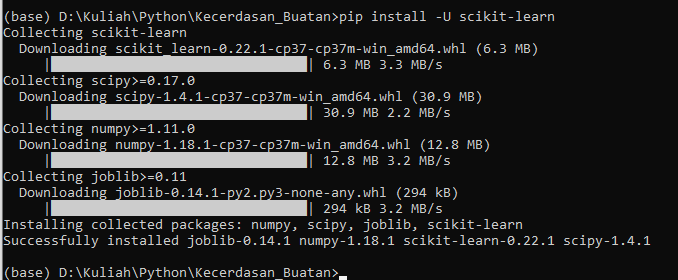
\includegraphics[width=4cm]{figures/1174035/chapter1/1_1.png}
		\centering
		\caption{Instalasi Scikit Learn}
	\end{figure}
	\item Setelah selesai instalasi, pilih salah satu example dari website Scikit (Contoh : \href{https://scikit-learn.org/stable/auto_examples/index.html})
	\begin{figure}[H]
		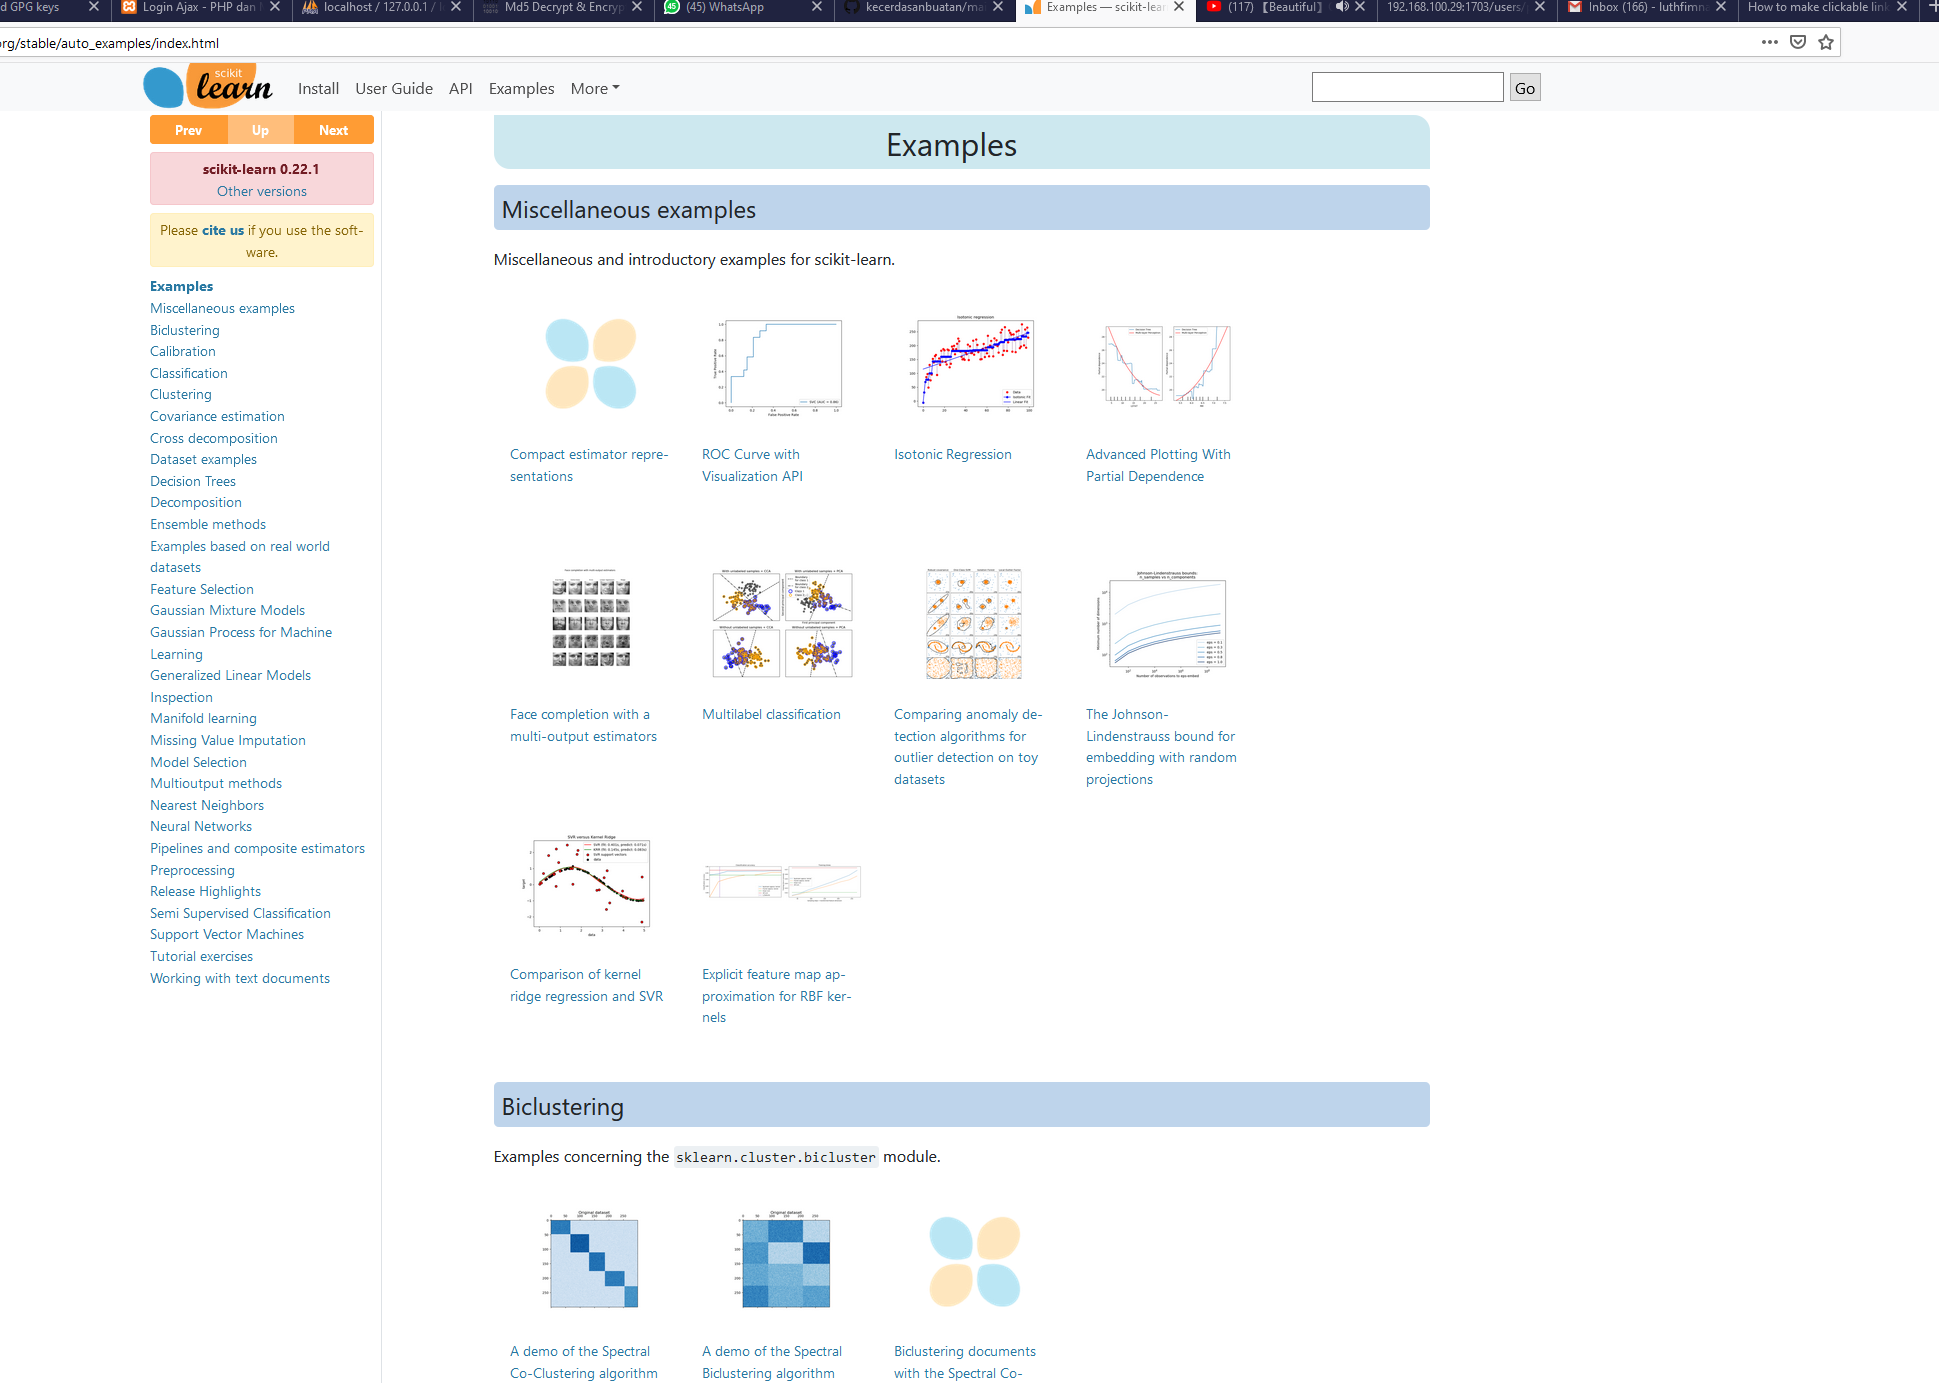
\includegraphics[width=4cm]{figures/1174035/chapter1/1_2.png}
		\centering
		\caption{Daftar Example}
	\end{figure}
	\item Lalu coba jalankan aplikasi tersebut, bisa dicek hasil dari Variable explorernya
	\begin{figure}[H]
		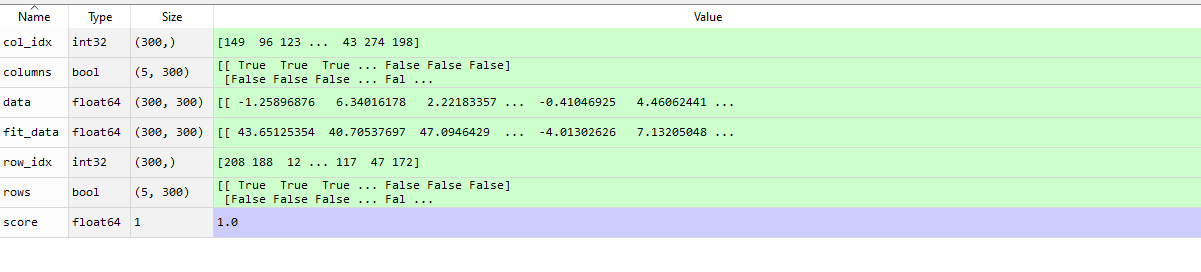
\includegraphics[width=4cm]{figures/1174035/chapter1/1_3.png}
		\centering
		\caption{Variable Explorer}
	\end{figure}
	\item Sample kode \hfill \break \lstinputlisting[firstline=1]{src/1174035/chapter1/sample1.py}
\end{enumerate}

\subsection{Mencoba Loading and example dataset}
Disini akan dilakukan percobaan dengan menggunakan beberapa datasets seperti digits dan iris untuk bisa digunakan sebagai training set yang akan dipakai seluruh metode.
\begin{itemize}
	\item Percobaan 1 (Memuat data iris dan digits dari datasets) \hfill \break \lstinputlisting[firstline=8, lastline=10]{src/1174035/chapter1/sample2.py}
	\begin{figure}[H]
		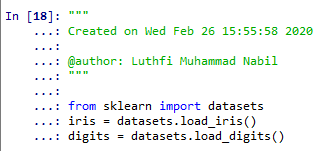
\includegraphics[width=4cm]{figures/1174035/chapter1/2_1_hasil.png}
		\centering
		\caption{Hasil Percobaan 1}
	\end{figure}
	\item Percobaan 2 (Menampilkan data dari digits) \hfill \break \lstinputlisting[firstline=12, lastline=12]{src/1174035/chapter1/sample2.py}
	\begin{figure}[H]
		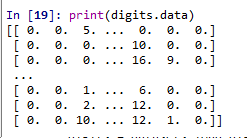
\includegraphics[width=4cm]{figures/1174035/chapter1/2_2_hasil.png}
		\centering
		\caption{Hasil Percobaan 2}
	\end{figure}
	\item Percobaan 3 (Menampilkan digits.target) \hfill \break \lstinputlisting[firstline=14, lastline=14]{src/1174035/chapter1/sample2.py}
	\begin{figure}[H]
		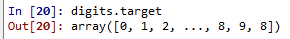
\includegraphics[width=4cm]{figures/1174035/chapter1/2_3_hasil.png}
		\centering
		\caption{Hasil Percobaan 3}
	\end{figure}
	\item Percobaan 4 (Menampilkan data 2 dimensi) \hfill \break \lstinputlisting[firstline=16, lastline=16]{src/1174035/chapter1/sample2.py}
	\begin{figure}[H]
		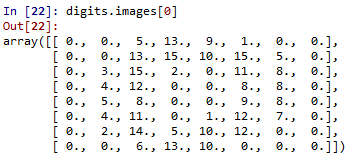
\includegraphics[width=4cm]{figures/1174035/chapter1/2_4_hasil.png}
		\centering
		\caption{Hasil Percobaan 4}
	\end{figure}
	\item Full sample \hfill \break \lstinputlisting[firstline=1]{src/1174035/chapter1/sample2.py}
	\begin{figure}[H]
		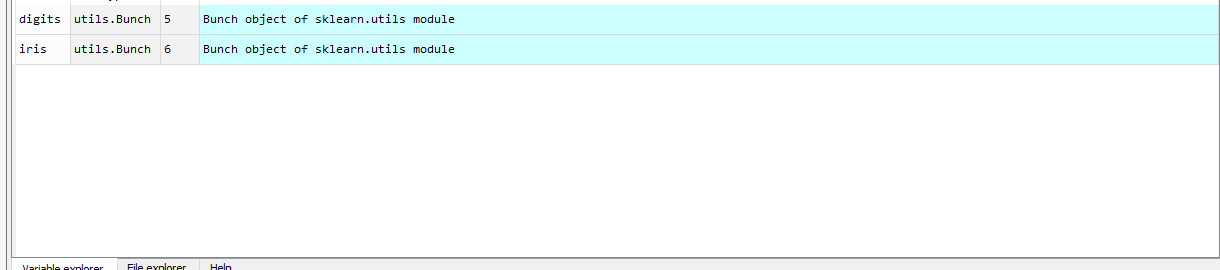
\includegraphics[width=4cm]{figures/1174035/chapter1/2_var.png}
		\centering
		\caption{Hasil pada variable explorer}
	\end{figure}
\end{itemize}
\subsection{Learning and Predicting}
Disini akan dicoba untuk melakukan prediksi berupa angka yang inputnya berupa gambaran dataset. 
\begin{itemize}
	\item Percobaan 1  \hfill \break \lstinputlisting[firstline=8, lastline=11]{src/1174035/chapter1/sample3.py}
	\begin{figure}[H]
		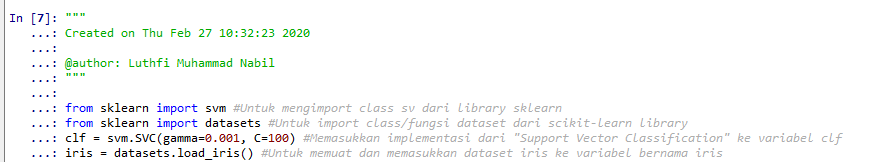
\includegraphics[width=4cm]{figures/1174035/chapter1/3_1_hasil.png}
		\centering
		\caption{Hasil Percobaan 1}
	\end{figure}
	\item Percobaan 2 \hfill \break \lstinputlisting[firstline=13, lastline=14]{src/1174035/chapter1/sample3.py}
	\begin{figure}[H]
		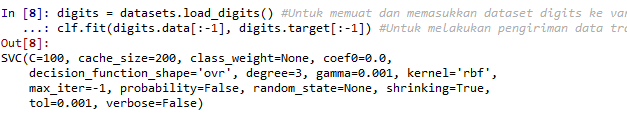
\includegraphics[width=4cm]{figures/1174035/chapter1/3_2_hasil.png}
		\centering
		\caption{Hasil Percobaan 2}
	\end{figure}
	\item Percobaan 3  \hfill \break \lstinputlisting[firstline=16, lastline=16]{src/1174035/chapter1/sample3.py}
	\begin{figure}[H]
		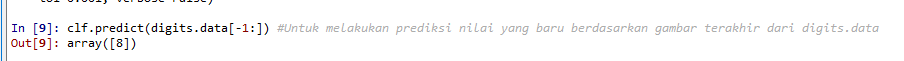
\includegraphics[width=4cm]{figures/1174035/chapter1/3_3_hasil.png}
		\centering
		\caption{Hasil Percobaan 3}
	\end{figure}
	\item Full sample \hfill \break \lstinputlisting[firstline=1]{src/1174035/chapter1/sample3.py}
	\begin{figure}[H]
		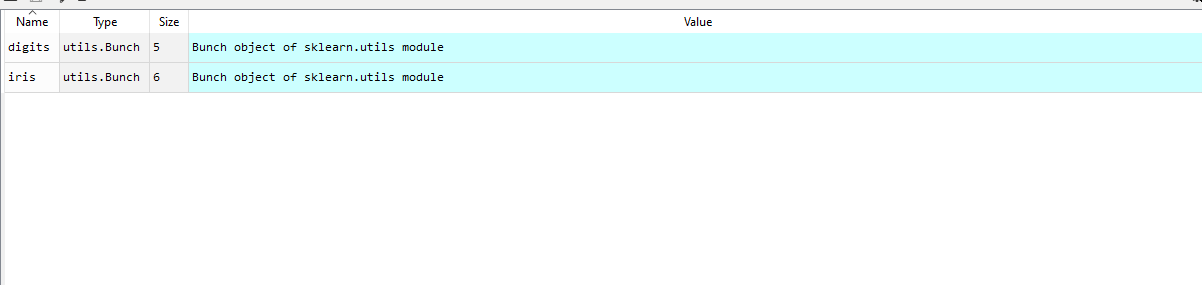
\includegraphics[width=4cm]{figures/1174035/chapter1/3_var.png}
		\centering
		\caption{Hasil pada variable explorer}
	\end{figure}
\end{itemize}
\subsection{Model Persistence}
Disini akan dilakukan persistensi model menggunakan built-in dari Python
\begin{itemize}
	\item Percobaan 1  \hfill \break \lstinputlisting[firstline=8, lastline=12]{src/1174035/chapter1/sample4.py}
	\begin{figure}[H]
		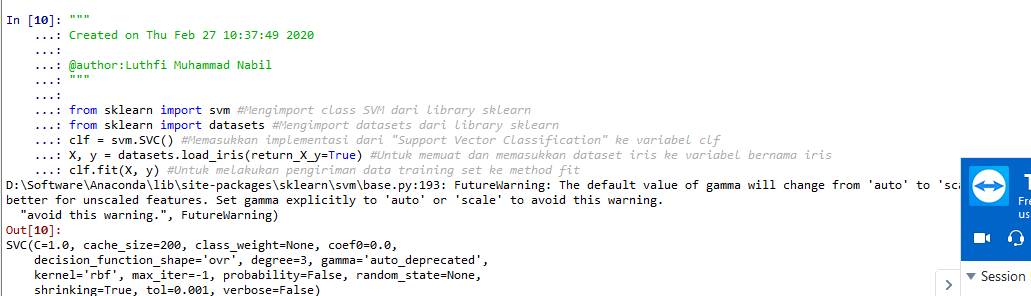
\includegraphics[width=4cm]{figures/1174035/chapter1/4_1_hasil.png}
		\centering
		\caption{Hasil Percobaan 1}
	\end{figure}
	\item Percobaan 2 \hfill \break \lstinputlisting[firstline=14, lastline=17]{src/1174035/chapter1/sample4.py}
	\begin{figure}[H]
		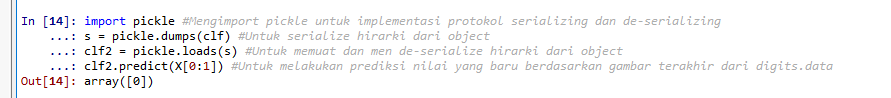
\includegraphics[width=4cm]{figures/1174035/chapter1/4_2_hasil.png}
		\centering
		\caption{Hasil Percobaan 2}
	\end{figure}
	\item Percobaan 3  \hfill \break \lstinputlisting[firstline=19, lastline=19]{src/1174035/chapter1/sample4.py}
	\begin{figure}[H]
		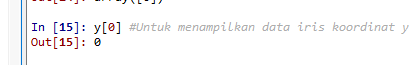
\includegraphics[width=4cm]{figures/1174035/chapter1/4_3_hasil.png}
		\centering
		\caption{Hasil Percobaan 3}
	\end{figure}
	\item Percobaan 4  \hfill \break \lstinputlisting[firstline=21, lastline=22]{src/1174035/chapter1/sample4.py}
	\begin{figure}[H]
		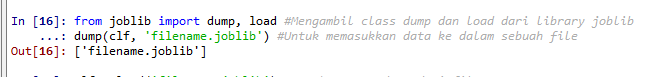
\includegraphics[width=4cm]{figures/1174035/chapter1/4_4_hasil.png}
		\centering
		\caption{Hasil Percobaan 4}
	\end{figure}
	\item Percobaan 5  \hfill \break \lstinputlisting[firstline=24, lastline=24]{src/1174035/chapter1/sample4.py}
	\begin{figure}[H]
		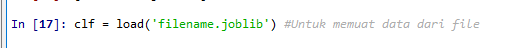
\includegraphics[width=4cm]{figures/1174035/chapter1/4_5_hasil.png}
		\centering
		\caption{Hasil Percobaan 5}
	\end{figure}
	\item Full sample \hfill \break \lstinputlisting[firstline=1]{src/1174035/chapter1/sample4.py}
	\begin{figure}[H]
		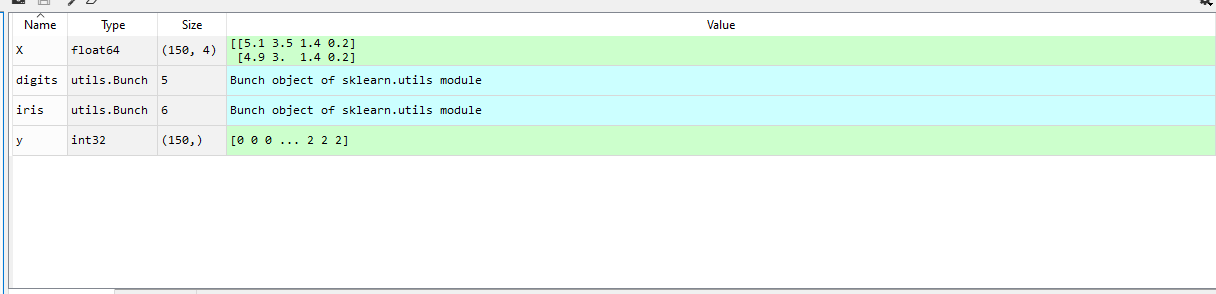
\includegraphics[width=4cm]{figures/1174035/chapter1/4_var.png}
		\centering
		\caption{Hasil pada variable explorer}
	\end{figure}
\end{itemize}
\subsection{Conventions}
Seluruh metode akan dilakukan pengaturan untuk membuat tingkah laku lebih dapat diprediksi
\begin{itemize}
	\item Percobaan 1  \hfill \break \lstinputlisting[firstline=8, lastline=14]{src/1174035/chapter1/sample5.py}
	\begin{figure}[H]
		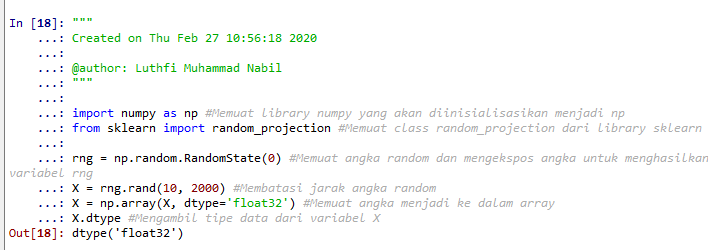
\includegraphics[width=4cm]{figures/1174035/chapter1/5_1_hasil.png}
		\centering
		\caption{Hasil Percobaan 1}
	\end{figure}
	\item Percobaan 2 \hfill \break \lstinputlisting[firstline=16, lastline=18]{src/1174035/chapter1/sample5.py}
	\begin{figure}[H]
		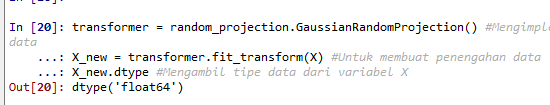
\includegraphics[width=4cm]{figures/1174035/chapter1/5_2_hasil.png}
		\centering
		\caption{Hasil Percobaan 2}
	\end{figure}
	\item Percobaan 3  \hfill \break \lstinputlisting[firstline=21, lastline=25]{src/1174035/chapter1/sample5.py}
	\begin{figure}[H]
		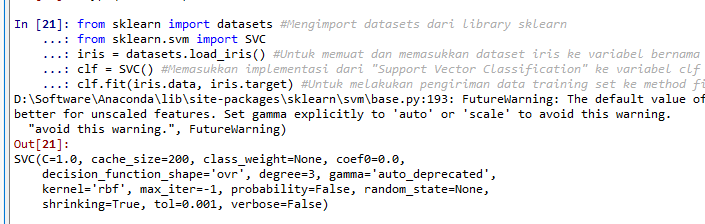
\includegraphics[width=4cm]{figures/1174035/chapter1/5_3_hasil.png}
		\centering
		\caption{Hasil Percobaan 3}
	\end{figure}
	\item Percobaan 4  \hfill \break \lstinputlisting[firstline=27, lastline=27]{src/1174035/chapter1/sample5.py}
	\begin{figure}[H]
		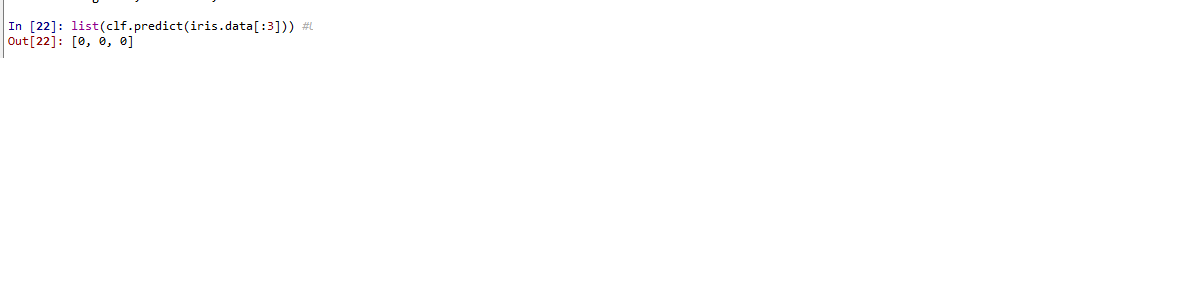
\includegraphics[width=4cm]{figures/1174035/chapter1/5_4_hasil.png}
		\centering
		\caption{Hasil Percobaan 4}
	\end{figure}
	\item Percobaan 5  \hfill \break \lstinputlisting[firstline=29, lastline=29]{src/1174035/chapter1/sample5.py}
	\begin{figure}[H]
		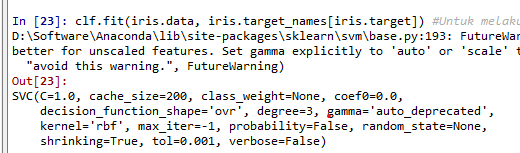
\includegraphics[width=4cm]{figures/1174035/chapter1/5_5_hasil.png}
		\centering
		\caption{Hasil Percobaan 5}
	\end{figure}
	\item Percobaan 6  \hfill \break \lstinputlisting[firstline=31, lastline=31]{src/1174035/chapter1/sample5.py}
	\begin{figure}[H]
		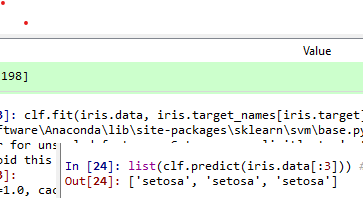
\includegraphics[width=4cm]{figures/1174035/chapter1/5_6_hasil.png}
		\centering
		\caption{Hasil Percobaan 6}
	\end{figure}
	\item Full sample \hfill \break \lstinputlisting[firstline=1]{src/1174035/chapter1/sample5.py}
	\begin{figure}[H]
		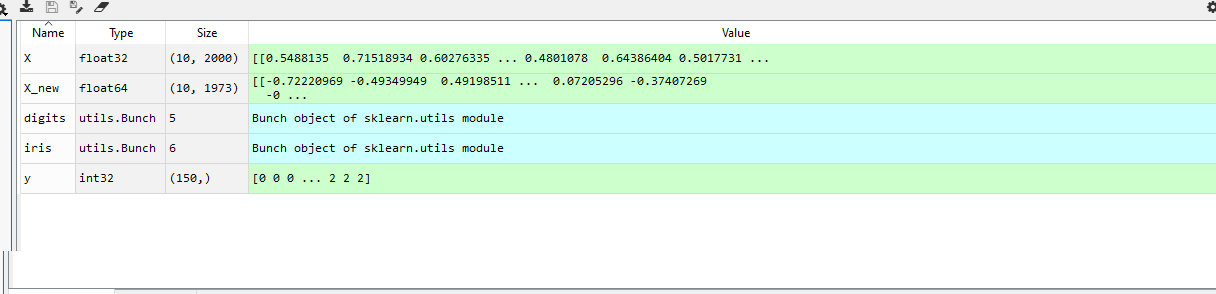
\includegraphics[width=4cm]{figures/1174035/chapter1/5_var.png}
		\centering
		\caption{Hasil pada variable explorer}
	\end{figure}
\end{itemize}
\subsection{Skrinsut Error}
\begin{figure}[H]
	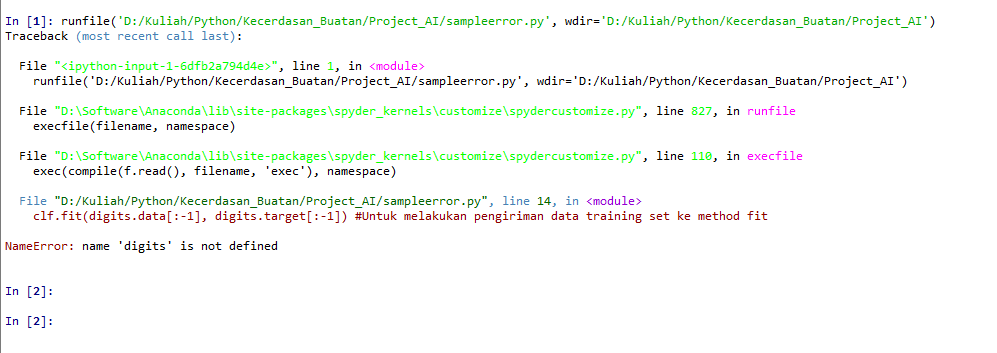
\includegraphics[width=4cm]{figures/1174035/chapter1/skrinsuterror.png}
	\centering
	\caption{Hasil Percobaan 6}
\end{figure}
\subsection{Kode error dan jenis error tersebut}
Error yang didapat berjenis name error, karena sebuah variabel tidak didefinisikan. Yaitu digits
\lstinputlisting[firstline=1]{src/1174035/chapter1/sample5.py}
\subsection{Penanganan Error}
Untuk menangani error tersebut, bisa ditambahkan sesuai instruksi. Yaitu menambahkan sebuah variabel bernama digits. Selain itu, digits harus dapat bekerja sebagaimana mestinya. Berikut full kodingnya : 
\lstinputlisting[firstline=1]{src/1174035/chapter1/sample3.py}
\subsection{Plagiarisme}
\begin{figure}[H]
	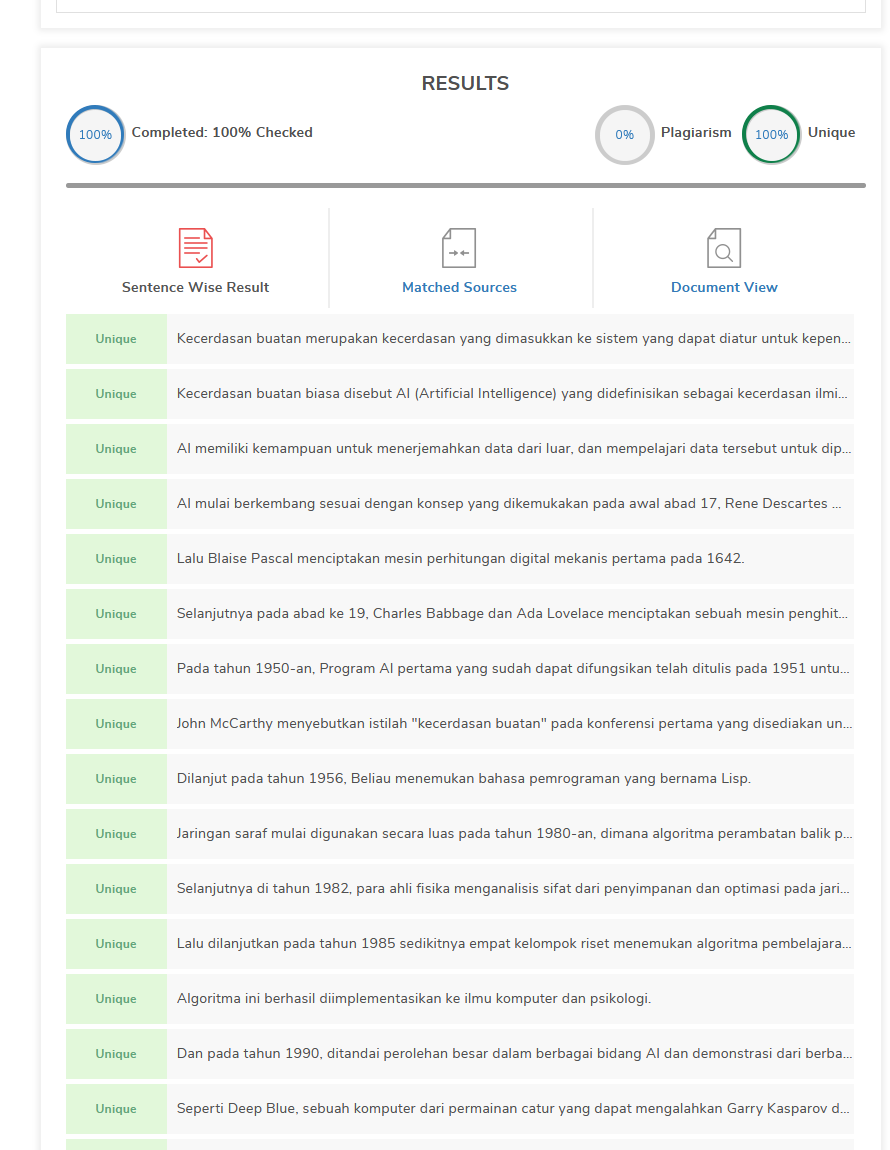
\includegraphics[width=4cm]{figures/1174035/chapter1/plagiarism.png}
	\centering
	\caption{Hasil pada variable explorer}
\end{figure}
\section{1174040 - Hagan Rowlenstino A. S}
    \subsection{Teori}
        \subsubsection{Definisi Kecerdasan Buatan}

        Artificial Inteligence atau dapat disebut juga dengan kecerdasan buatan merupakan kecerdasan yang ditambahakn kepada suatu sistem yang dapat diatur dalam konteks ilmiah.Michael Haenlein dan Andreas Kaplan mendefinisikan bahawa AI adalah “kemampuan sebuah sistem untuk menejerjemahkan data eksternal dengan benar, mempelajari data tersebut, dan menggunakannya guna mencapai tujuan dan tugas tertentu melalui adaptasi yang fleksibel”. Kecerdasan ini dibuat dan dimasukkan ke dalam mesin agar dapat melakukan pekerjaan seperti yang dapat dilakukan manusia dengan cepat dan tepat. Bidang- bidang yang menggunakan kecerdasan buatan antara lain logika fuzzy, permainan komputer (games), sistem pakar, jaringan saraf tiruan dan robotika.
        
        \subsubsection{Sejarah Kecerdasan Buatan}
        
        Sejarah kecerdasan buatan ini dimulai dari zaman kuno, mitos ataupun cerita dan desas-desus tentang sebuah mahkluk yang mempunyai kecerdasan serta kesadaran yang diberikan oleh pengrajin. Benih - benih nya mulai ditanam oleh para filsuf klasik yang mencari cara untuk menggambarkan proses berfikir manusia sebagai manipulasi simbol secara mekanis yang memuncah pada penemuan komputer digital di tahun 1940-an, yaitu sebuah mesin yang didasarkan penalaran matematika. Istilah kecerdasan buatan sendiri baru muncul pada tahun 1956, dan teori -teori nya sudah muncul sejak tahun 1941.

        \subsubsection{Perkembangan Kecerdasan Buatan}
        \begin{enumerate}
            \item Perkembangan kecerdasan buatan dimulai dari Era Komputer Elektronik pada tahun 1941. dimana ditemukannya alat penyimpanan dan pemrosesan informasi. Dilanjutkan pada tahun 1949, berhasilnya pembuatan komputer yang mampu menyimpan program yang memunat pekerjaan dalam memasukkan program menjadi lebih mudah.
            \item Masa - masa persiapan AI terjadi pada tahun 1943 - 1956.
            \item Awal Perkembangan AI terjadi pada 1952 - 1969
            \item Perkembagan kecerdasan buatan melambat pada tahun 1966-1974
            \item Sistem Berbasis Pengetahuan pada tahun 1969-1979
            \item ecerdasan Buatan menjadi sebuah industri pada tahun 1980-1988. Kembalinya Jaringan Syaraf tiruan pada tahun 1986-sekarang.
        \end{enumerate}
    \subsection{Instalasi}
        Membuka  https://scikit-learn.org/stable/tutorial/basic/tutorial.html lalu mencobanya.
        \subsubsection{Instalasi library scikit, mencoba kompilasi dan ujicoba contoh kode}
        \begin{enumerate}
            \item Buka anaconda prompt lalu ketikkan "pip install -U scikit-learn" untuk menginstall library scikit
            \begin{figure}[H]
                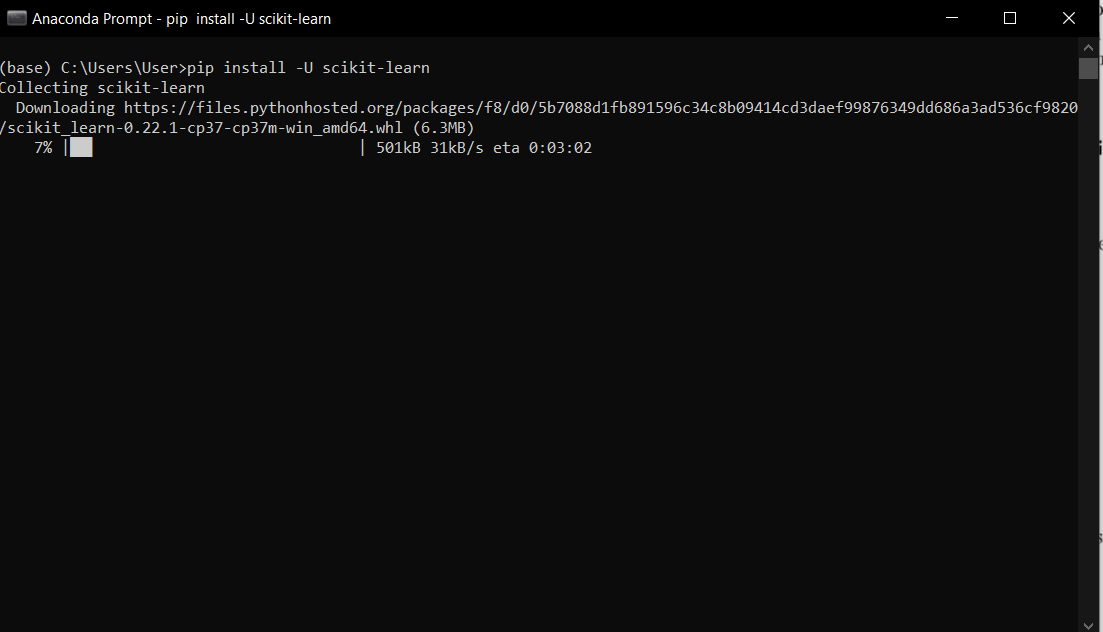
\includegraphics[width=4cm]{figures/1174040/chap1/1.png}
                \centering
                \caption{Install Library Scikit}
            \end{figure}
            \item Pilih salah satu example dari website tersebut lalu jalankan \hfill \break \lstinputlisting[firstline=1]{src/1174040/chap1/ex1.py}
            
            \item buka variable explolernya
            \begin{figure}[H]
                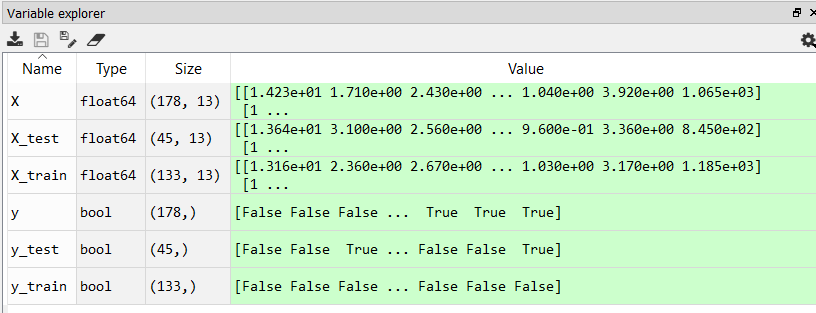
\includegraphics[width=4cm]{figures/1174040/chap1/2.png}
                \centering
                \caption{Variable Exploler}
            \end{figure}
        \end{enumerate}
        \subsubsection{Mencoba loading an example dataset}
        \begin{enumerate}
            \item mengambil data iris dan digit dari dataset \hfill \break \lstinputlisting[firstline=9, lastline=11]{src/1174040/chap1/ex2.py}
            
            \item Menampilkan data digits \hfill \break \lstinputlisting[firstline=13, lastline=13]{src/1174040/chap1/ex2.py}
            
            \begin{figure}[H]
                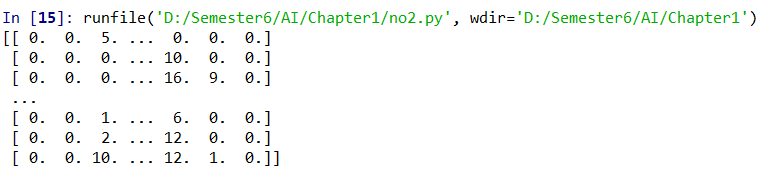
\includegraphics[width=4cm]{figures/1174040/chap1/3.png}
                \centering
                \caption{Data Digits}
            \end{figure}

            \item menampilkan digits.target
            \hfill \break \lstinputlisting[firstline=15, lastline=15]{src/1174040/chap1/ex2.py}

            \begin{figure}[H]
                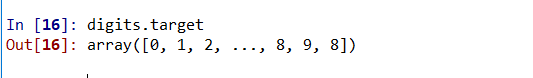
\includegraphics[width=4cm]{figures/1174040/chap1/4.png}
                \centering
                \caption{Digits Target}
            \end{figure}

            \item menampilkan data bentuk 2D. \hfill \break \lstinputlisting[firstline=17, lastline=17]{src/1174040/chap1/ex2.py}

            \begin{figure}[H]
                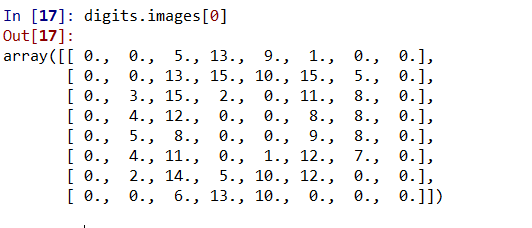
\includegraphics[width=4cm]{figures/1174040/chap1/5.png}
                \centering
                \caption{Data 2D}
            \end{figure}
        \end{enumerate}
\section{1174042 Faisal Najib Abdullah}
\subsection{Teori}
\begin{enumerate}
\item Definisi, sejarah, dan perkembangan kecerdasan buatan.
\subitem Definisi kecerdasan buatan adalah suatu pengetahuan yang dapat membuat komputer untuk meniru kecerdasan manusia yang berhubungan dengan penangkapan, pemodelan, dan penyimpanan kecerdasan manusia dalam sebuah sistem teknologi. Contohnya yaitu melakukan analisa penalaran untuk mengambil suatu kesimpulan atau penerjemahan atau keputusan dari satu bahasa satu ke bahasa lain.
\subitem Sejarah dan perkembangan kecerdasan buatan terjadi pada musim panas tahun 1956 tercatat adanya seminar mengenai AI di Darmouth College. Seminar pada waktu itu dihadiri oleh sejumlah pakar komputer dan membahas potensi komputer dalam meniru kepandaian manusia. Akan tetapi perkembangan yang sering terjadi semenjak diciptakannya LISP, yaitu bahasa kecerdasan buatan yang dibuat tahun 1960 oleh John McCarthy. Istilah pada kecerdasan buatan atau Artificial Intelligence diambil dari Marvin Minsky dari MIT. Dia menulis karya ilmiah berjudul Step towards Artificial Intelligence, The Institute of radio Engineers Proceedings 49, January 1961\cite{baraja2008kecerdasan}. 
\item  Definisi supervised learning, klasifikasi, regresi, dan unsupervised learning. Data set, training set dan testing set. 
\subitem Supervised learning merupakan sebuah pendekatan dimana sudah terdapat data yang dilatih, dan terdapat variable yang ditargetkan sehingga tujuan dari pendekatan ini adalah mengkelompokan suatu data ke data yang sudah ada. Sedangkan unsupervised learning tidak memiliki data latih, sehingga dari data yang ada, kita mengelompokan data tersebut menjadi 2 bagian atau 3 bagian dan seterusnya.
\subitem Klasifikasi adalah salah satu topik utama dalam data mining atau machine learning. Klasifikasi yaitu suatu pengelompokan data dimana data yang digunakan tersebut mempunyai kelas label atau target.
\subitem Regresi adalah Supervised learning tidak hanya mempelajari classifier, tetapi juga mempelajari fungsi yang dapat memprediksi suatu nilai numerik. Contoh, ketika diberi foto seseorang, kita ingin memprediksi umur, tinggi, dan berat orang yang ada pada foto tersebut.
\subitem Data set adalah cabang aplikasi dari Artificial Intelligence/Kecerdasan Buatan yang fokus pada pengembangan sebuah sistem yang mampu belajar sendiri tanpa harus berulang kali di program oleh manusia.
\subitem Training set yaitu jika pasangan objek, dan kelas yang menunjuk pada objek tersebut adalah suatu contoh yang telah diberi label akan menghasilkan suatu algoritma pembelajaran.
\subitem Testing set digunakan untuk mengukur sejauh mana classifier berhasil melakukan klasifikasi dengan benar\cite{zhu2009introduction}.
\end{enumerate}

\subsection{Instalasi}
\subsubsection{Instalasi Library Scikit dari Pycharm}
Masuk pada menu settings terus pilih Project Interpreter kemudian tambah library lalu cari dan install scikit
\begin{figure}[ht]
\centering
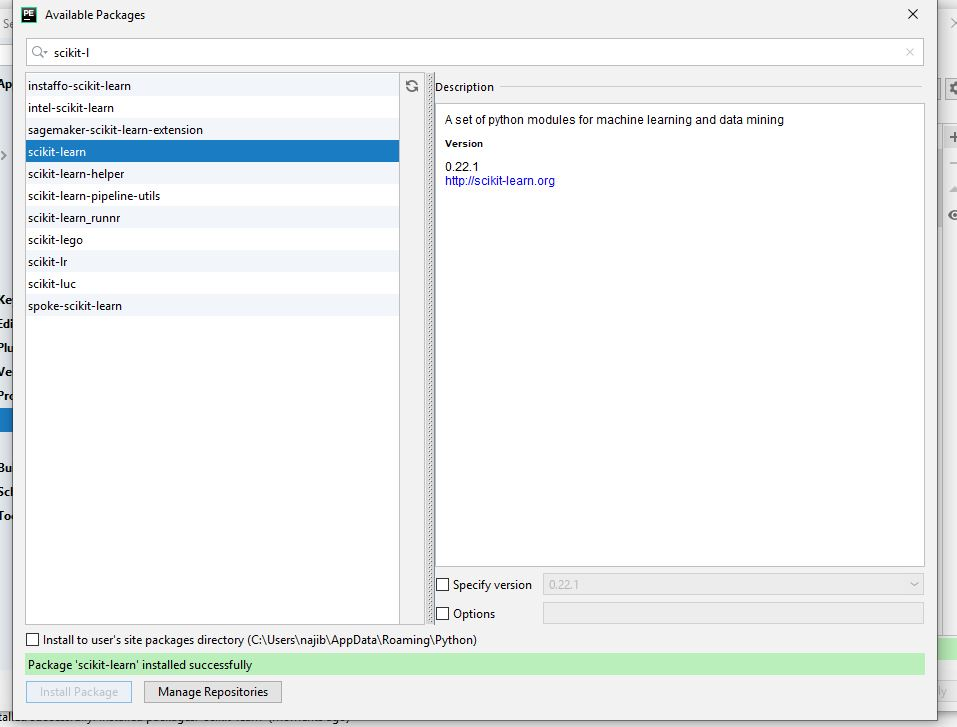
\includegraphics[scale=0.5]{figures/1174042/chapter1/2.jpg}
\caption{Installasi}
\label{contoh}
\end{figure}

Mencoba Library
\lstinputlisting{src/1174042/chapter1/2,1.py}

\subsubsection{Mencoba Loading an example Dataset}
\lstinputlisting{src/1174042/chapter1/2,2.py}
\begin{figure}[ht]
\centering
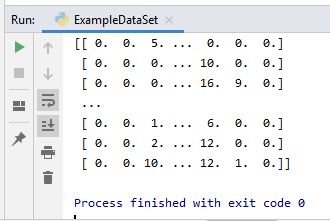
\includegraphics[scale=0.5]{figures/1174042/chapter1/3.jpg}
\caption{Mencoba Loading an example Dataset}
\label{contoh}
\end{figure}

\subsubsection{Learning and Predicting}
\lstinputlisting{src/1174042/chapter1/2,3.py}
\begin{figure}[ht]
\centering
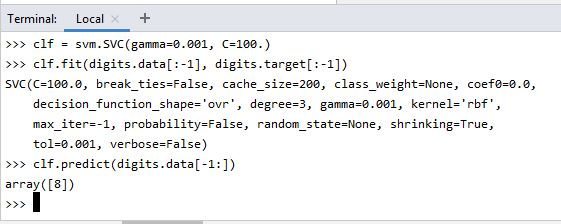
\includegraphics[scale=0.5]{figures/1174042/chapter1/2,3.jpg}
\caption{Learning and Predicting}
\label{contoh}
\end{figure}

\subsubsection{Model Presistence}
\lstinputlisting{src/1174042/chapter1/2,4.py}
\begin{figure}[ht]
\centering
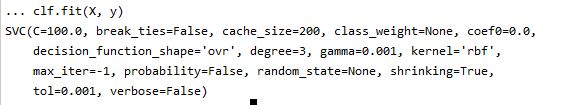
\includegraphics[scale=0.5]{figures/1174042/chapter1/2,4.jpg}
\caption{Model Presistence}
\label{contoh}
\end{figure}

\begin{figure}[ht]
\centering
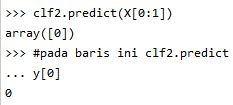
\includegraphics[scale=0.5]{figures/1174042/chapter1/2,4,1.jpg}
\caption{Model Presistence}
\label{contoh}
\end{figure}

\begin{figure}[ht]
\centering
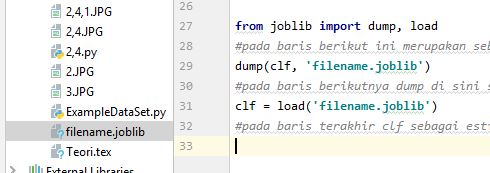
\includegraphics[scale=0.5]{figures/1174042/chapter1/2,4,2.jpg}
\caption{Model Presistence}
\label{contoh}
\end{figure}

\subsubsection{Conventions}
\lstinputlisting{src/1174042/chapter1/2,5.py}


\subsection{Penanganan eror}
\subsubsection{ScreenShoot Eror}
\begin{figure}[ht]
\centering
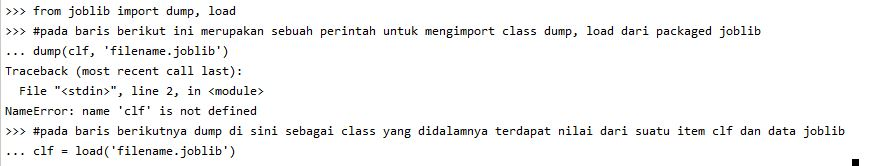
\includegraphics[scale=0.5]{figures/1174042/chapter1/3,1.jpg}
\caption{Error}
\label{contoh}
\end{figure}

\subsubsection{Tuliskan Kode Eror dan Jenis Erornya}
\begin{verbatim}
File "<stdin>", line 2, in <module>
NameError: name 'clf' is not defined
\end{verbatim}


\subsubsection{Solusi Pemecahan Masalah Error}
Ini karna kode di jalankan perbaris perbaris, jika kode dijanlankan bersamaan makan kode berjan sesuai prosedur.

\subsection{Plagiat}
\begin{figure}[ht]
\centering
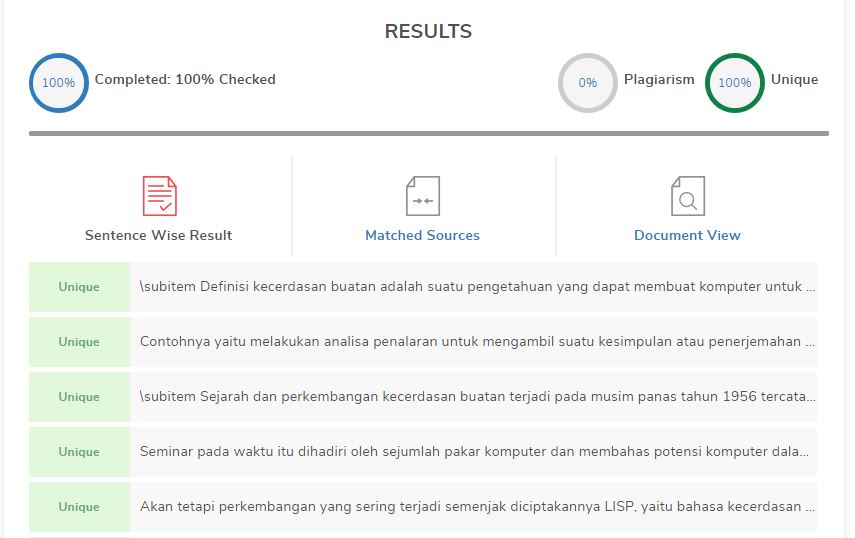
\includegraphics[scale=0.5]{figures/1174042/chapter1/5.jpg}
\caption{Error}
\label{contoh}
\end{figure}
\section{1174043 - Irvan Rizkiansyah}
	\subsection {Definisi Kecerdasan Buatan}
	Kecerdasan buatan atau biasa disebut AI (Artificial Intelligence) merupakan kecerdasan yang dibuat dan ditambahkan oleh manusia ke suatu sistem teknologi, yang diatur dan dikembangkan dalam konteks ilmiah, yang merupakan bentukan dari kecerdasan entitas ilmiah yang ada. Jadi pada intinya definisi AI dapat terus dikembangkan, namun yang menjadi poin utamanya adalah bagaimana manusia menciptakan sebuah teknologi yang dapat berpikir seperti selayaknya manusia itu sendiri.
	
	\subsection{Sejarah dan Perkembangan}
	\begin{itemize}
		\item Program kecerdasan buatan atau Artificial Intelligence pertama kali dicetuskan pada kisaran tahun 1951. Tidak bisa dipungkiri bahwa di tahun tersebut memang sedang gencar-gencarnya pembuatan cikal bakal, konsep, hingga teknologi berbasis AI. Dan, AI sendiri pertama kali digunakan di University of Manchester untuk menjalankan sebuah mesin bernama Ferranti Mark 1.
		\item Beberapa waktu kemudian, Christopher Strachey melanjutkan konsep kecerdasan buatan untuk menjalankan sebuah permainan catur, dimana bidak catur tersebut dapat berjalan secara otomatis dan mampu bermain melawan manusia sungguhan.
		\item Berlanjut pada tahun 1956, kecerdasan buatan tidak hanya dibuat untuk memudahkan bermain catur saja. Melainkan pada saat konferensi pertamanya, John McCharty menamai algoritma teknologi tersebut dengan sebutan “Artificial Intelligence”. Istilah tersebut masih digunakan hingga sekarang oleh para pakar teknologi.
		\item Terakhir, konsep dan teknologi kecerdasan buatan disempurnakan oleh seorang ahli yang namanya masih diingat sampai sekarang sebagai seorang pakar kecerdasan buatan, yaitu Alan Turin. Pada saat itu, Alan Turin meneliti dan menguji coba algoritma AI yang diberi nama dengan “Turing Test”. Hingga seiring berkembangnya waktu, konsep teknologi AI banyak digunakan di berbagai teknologi baik itu multimedia, search engine, dan masih banyak lainnya.
	\end{itemize}
	
	\subsection{Supervised Learning}
	Supervised learning (Pembelajaran terawasi), dalam konteks kecerdasan buatan (AI) dan Machine Learning, adalah jenis sistem di mana input dan output data yang diinginkan disediakan. Input dan output data diberi label untuk klasifikasi untuk memberikan dasar pembelajaran untuk pemrosesan data di masa depan.
	
	\subsection{Unsupervised Learning}
	Unsupervised learning merupakan pembelajan yang tidak terawasi dimana tidak memerlukan target output. Pada metode ini tidak dapat ditentukan hasil seperti apa yang diharapkan selama proses pembelajaran, nilai bobot yang disusun dalam proses range tertentu tergantung pada nilai output yang diberikan. Tujuan metode uinsupervised learning ini agar kita dapat mengelompokkan unit-unit yang hampir sama dalam satu area tertentu.
	
	\subsection{Teknik Klasifikasi}
	Teknik klasifikasi memprediksi respons diskrit, misalnya seperti apakah email itu asli atau spam, atau apakah tumor itu kanker atau tidak. Model klasifikasi mengklasifikasikan data masukan ke dalam kategori tersebut.
	
	\subsection{Regresi}
	Regresi yaitu pengeluaran nilai output yang konstan jika dipicu dengan parameter tertentu biasanya regresi disini berbentuk regresi linier. Regresi linier yaitu metode statistika yang digunakan untuk membentuk model hubungan antara variabel terikat(dependen,respon,Y) dengan satu atau lebih variabel bebas(independent, prdiktor, X). Apabila banyaknya variabel bebas hanya ada satu, disebut sebagai regresi linier sederhana, sedangkan apabila terdapat lebih dari satu variabel bebas, disebut sebagai regresi linier berganda.
	
	\subsection{Training Set}
	Training set adalah bagian dari dataset itu sendiri yang dilatih untuk membuat prediksi atau algoritma mesin learning lainnya sesuai keinginan atau tujuan data itu dibuat.
	
	\subsection{Testing Set}
	Testing set adalah bagian dari dataset yang di tes atau diujicoba untuk melihat keakuratannya dengan katalain melihat peformanya.
	
	\subsection{Instalasi dan Percobaan Kompilasi dari Library Scikit-learn}
	\begin{enumerate}
		\item Buka anaconda prompt
		\item kemudian Ketik di anaconda prompt yaitu : "pip install -U scikit-learn" \break
		\begin{figure}[H]
			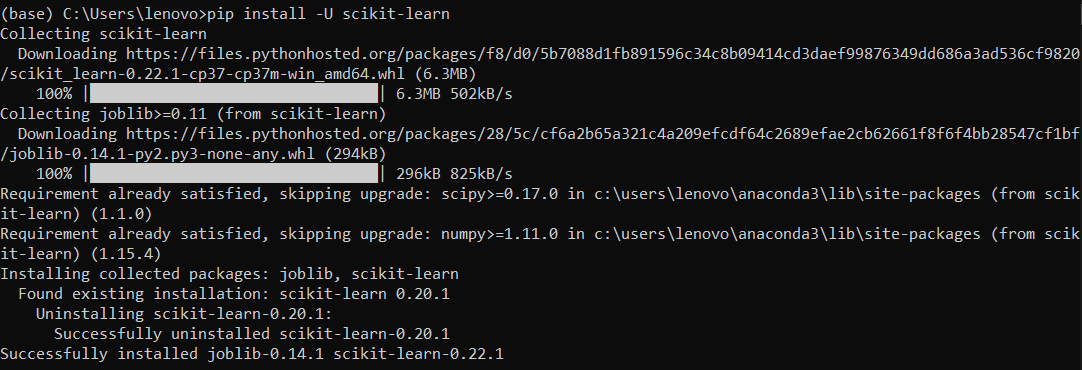
\includegraphics[width=4cm]{figures/1174043/chapter1/1.png}
			\centering
			\caption{Instalasi Scikit Learn}
		\end{figure}
		\item Setelah selesai instalasi, pilih salah satu example dari website Scikit
		\item Sample kode \break \lstinputlisting[firstline=1]{src/1174043/chapter1/sample1.py}
		\item Kemudian jalankan aplikasi tersebut, dan bisa dicek hasil dari Variable explorernya \break
		\begin{figure}[H]
			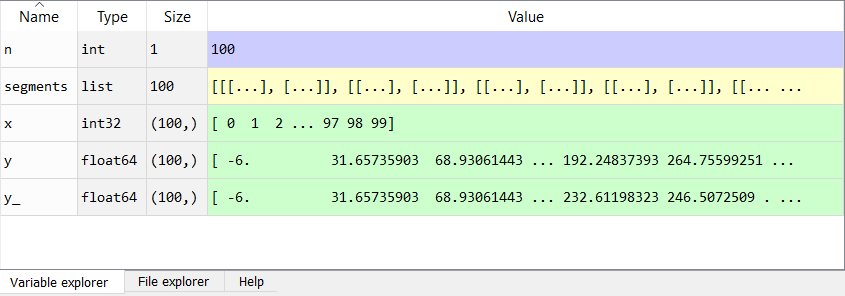
\includegraphics[width=4cm]{figures/1174043/chapter1/hasil_sample.png}
			\centering
			\caption{Variable Explorer}
		\end{figure}
	\end{enumerate}
	
	\subsection{Mencoba Loading an example dataset}
	\begin{enumerate}
		\item Sample kode \break \lstinputlisting[firstline=1]{src/1174043/chapter1/sample2.py}
		\item Kemudian jalankan aplikasi tersebut \break
		\begin{figure}[H]
			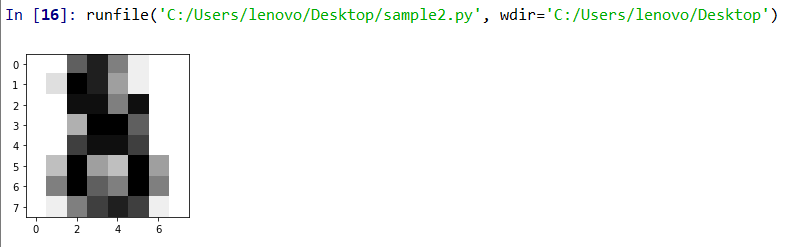
\includegraphics[width=4cm]{figures/1174043/chapter1/hasil_dataset.png}
			\centering
			\caption{Dataset}
		\end{figure}
	\end{enumerate}
\section{1174050 Dika Sukma Pradana}
\subsection{Teori}
\begin{enumerate}
\item Definisi, sejarah, dan perkembangan kecerdasan buatan.
\subitem Intelegensi buatan (AI) mengacu pada simulasi kecerdasan manusia dalam mesin yang diprogram untuk berpikir seperti manusia dan meniru tindakan mereka. Istilah ini juga dapat diterapkan pada mesin apa pun yang menunjukkan sifat-sifat yang terkait dengan pikiran manusia seperti pembelajaran dan pemecahan masalah.
\subitem Sejarah Kecerdasan Buatan (AI) bermula pada saat zaman kuno, dengan sejuta mitos, cerita dan desas-desus tentang makhluk buatan yang diberkahii dengan kecerdasan oleh pengrajin ahli. Benih-benih AI modern ditanam oleh para filsuf klasik yang mencoba menggambarkan proses pemikiran manusia sebagai manipulasi simbol secara mekanis. Karya ini memuncak dalam penemuan komputer digital yang dapat diprogram pada tahun 1940-an, sebuah mesin yang didasarkan pada esensi abstrak penalaran matematika. Perangkat ini dan ide-ide di belakangnya menginspirasi segelintir ilmuwan untuk mulai serius membahas kemungkinan membangun otak elektronik.
Bidang penelitian AI didirikan pada lokakarya yang diadakan di kampus Dartmouth College selama musim panas 1956. Mereka yang hadir akan menjadi pemimpin penelitian AI selama beberapa dekade. Banyak dari merekka meramaIkan bahwa sebuah mesin yang secerdas manusia akan hidup tidak lebih dari satu generasi dan mereka diberi jutaan dolar untuk mewujudkan visi atau tujuan ini.
Akhirnya, menjadi jelas bahwa mereka meremehkan kesulitan proyek. Pada tahun 1973, sebagai tanggapan atas kritik dari James Lighthill dan tekanan terus-menerus dari kongres, AS dan Pemerintah Inggris menghentikan pendanaan penelitian yang tidak diarahkan pada kecerdasan buatan, dan tahun-tahun sulit berikutnya akan dikenal sebagai musim dingin AI. Tujuh tahun kemudian, sebuah inisiatif visioner oleh Pemerintah Jepang mengilhami pemerintah dan industri untuk menyediakan miliaran dolar dalam AI, tetapi pada akhir 80-an investor menjadi kecewa dengan kurangnya daya komputer (perangkat keras) yang dibutuhkan dan menarik lebih banyak dana.
Investasi dan minat pada AI tumbuh pesat pada dekade pertama abad ke-21, ketika pembelajaran mesin berhasil diterapkan pada banyak masalah di dunia akademis dan industri karena metode baru, penerapan perangkat keras komputer yang kuat, dan kumpulan data yang sangat besar.
\item  Definisi supervised learning, klasifikasi, regresi, dan unsupervised learning. Data set, training set dan testing set. 
\subitem Supervised learning adalah sebuah metode pendekatan yang mana sudah terdapat data yang dilatiih, dan terdapat variabel yang ditargetkan atau yang menjadi tujuan sehingga tujuan dari pendekatan ini adalah mengkelompokan suatu data ke data yang sudah ada. Sedangkan unsupervised learrning tidak memiliki data latiih, sehinggga dari data yang ada, kita mengelompokan data tersebbut menjadi dua bagian atau bahkan tiga bagian dan seterusnya.
\subitem Klasifikasi adalah salah satu topik utama dalam data mining atau machine learning. Klasifikasi yaitu suatu pengelompokan data dimana data yang digunakan tersebut mempunyai kelas label atau target.
\subitem Regresi adalah Supervised learning tidak hanya mempelajari classifier, tetapi juga mempelajari fungsi yang dapat memprediksi suatu nilai numerik. 
\subitem Data set merupakan sebuah cabang aplikasi dari Artificial Intelligence(AI)/Kecerdasan Buatan yang terfokus kepada pengembangan sebuah sistem yang mampu belajar sendiiri tannpa harus berulang kalai di program oleh manusia(programmer).
\subitem Training set yaitu jika pasangan objek, dan kelas yang menunjuk pada objek tersebut adalah suatu contoh yang telah diberi label akan menghasilkan suatu algoritma pembelajaran.
\subitem Testing set digunakan untuk mengukur sejauh mana classifier berhasil melakukan klasifikasi dengan benar\cite{zhu2009introduction}.
\end{enumerate}

\subsection{Instalasi}
\subsubsection{Instalasi Library Scikit dari Anaconda}
\begin{enumerate}
\item Download aplikasi Anaconda terlebih dahulu. 
\item Install aplikasi Anaconda yang sudah di download tadi. 
\item Simpan aplikasi sesuai folder yang kita pilih lalu next. 
\item Centang Keduanya lalu tekan tombol install. 
\item Setelah itu tunggu sampai proses instalasi selesai lalu jika sudah tekan tombol finish. 
\item Lalu buka command prompt anda dan tuliskan perintah berikut ini untuk mengecek apakah aplikasinya sudah terinstall. 
\item Kemudian ketikkan perinta pip install -U scikit-learn seperti gambar berikut. 
\end{enumerate}
         \begin{figure}[H]
                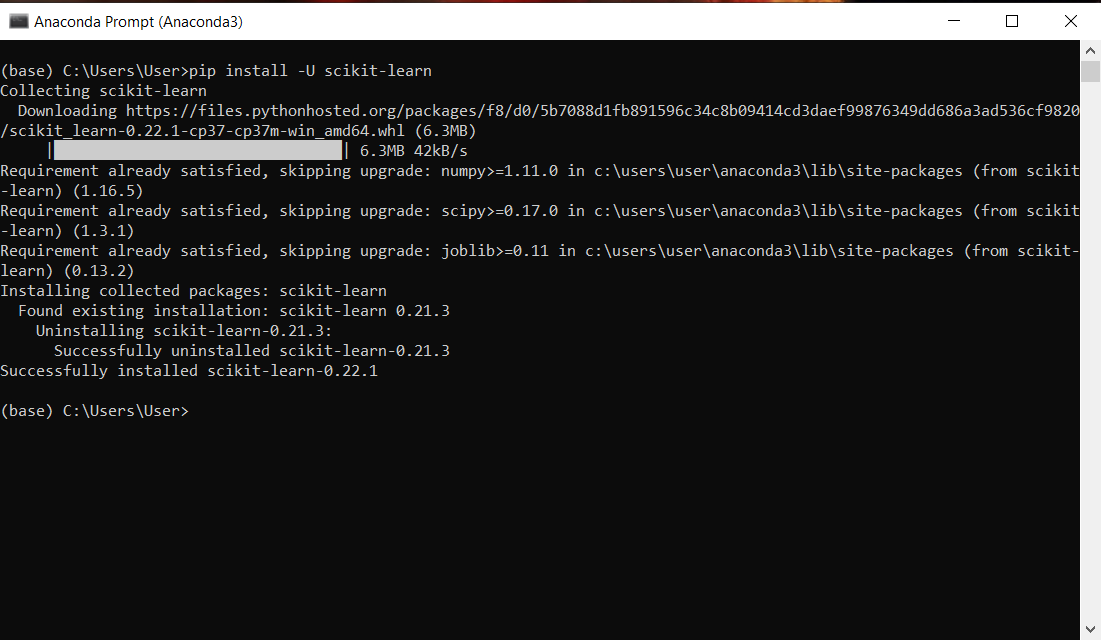
\includegraphics[width=4cm]{figures/1174050/chapter1/instal.png}
                \centering
                \caption{Instalasi}
            \end{figure}


\subsection{Percobaan}
Mencoba Library
\lstinputlisting{src/1174050/chapter1/VAR.py}
 \begin{figure}[H]
                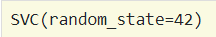
\includegraphics[width=4cm]{figures/1174050/chapter1/2.png}
                \centering
                \caption{Variabel Explore}
            \end{figure}


\subsubsection{Mencoba Loading an example Dataset}
\lstinputlisting{src/1174050/chapter1/dataset.py}
 \begin{figure}[H]
                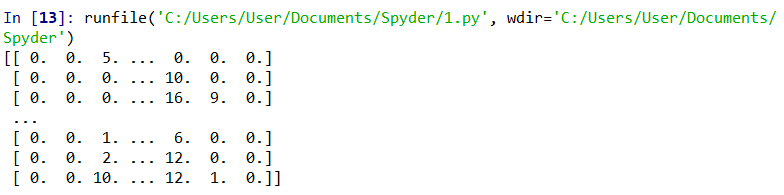
\includegraphics[width=4cm]{figures/1174050/chapter1/1.png}
                \centering
                \caption{Datasets}
            \end{figure}


\subsubsection{Learning and Predicting}
\lstinputlisting{src/1174050/chapter1/learning.py}


\subsubsection{Model Presistence}
\lstinputlisting{src/1174050/chapter1/modelpersistance.py}


\subsubsection{Conventions}
Type Casting
\lstinputlisting{src/1174050/chapter1/typecasting.py}
Refitting and updating parameters
\lstinputlisting{src/1174050/chapter1/Multiclass.py}
Multiclass vs. multilabel fitting
\lstinputlisting{src/1174050/chapter1/Refitting.py}


\subsection{Penanganan eror}
\subsubsection{ScreenShoot Eror}
\begin{figure}[ht]
\centering
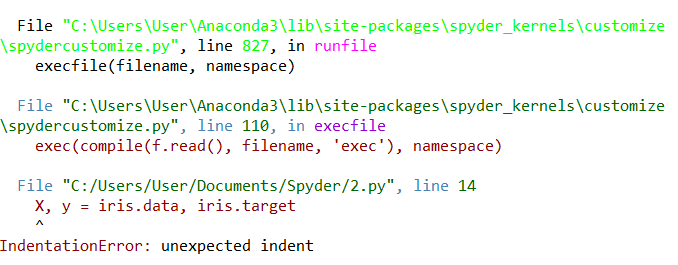
\includegraphics[scale=0.5]{figures/1174050/chapter1/error.png}
\caption{Error}
\label{contoh}
\end{figure}

\subsubsection{Tuliskan Kode Eror dan Jenis Erornya}
\begin{verbatim}
IndentationError: unexpected indent
\end{verbatim}


\subsubsection{Solusi Pemecahan Masalah Error}
Pastikan semua spasi pada koding sama. Menggunakan spasi atau tab.

\subsection{Plagiarism}
\begin{figure}[ht]
\centering
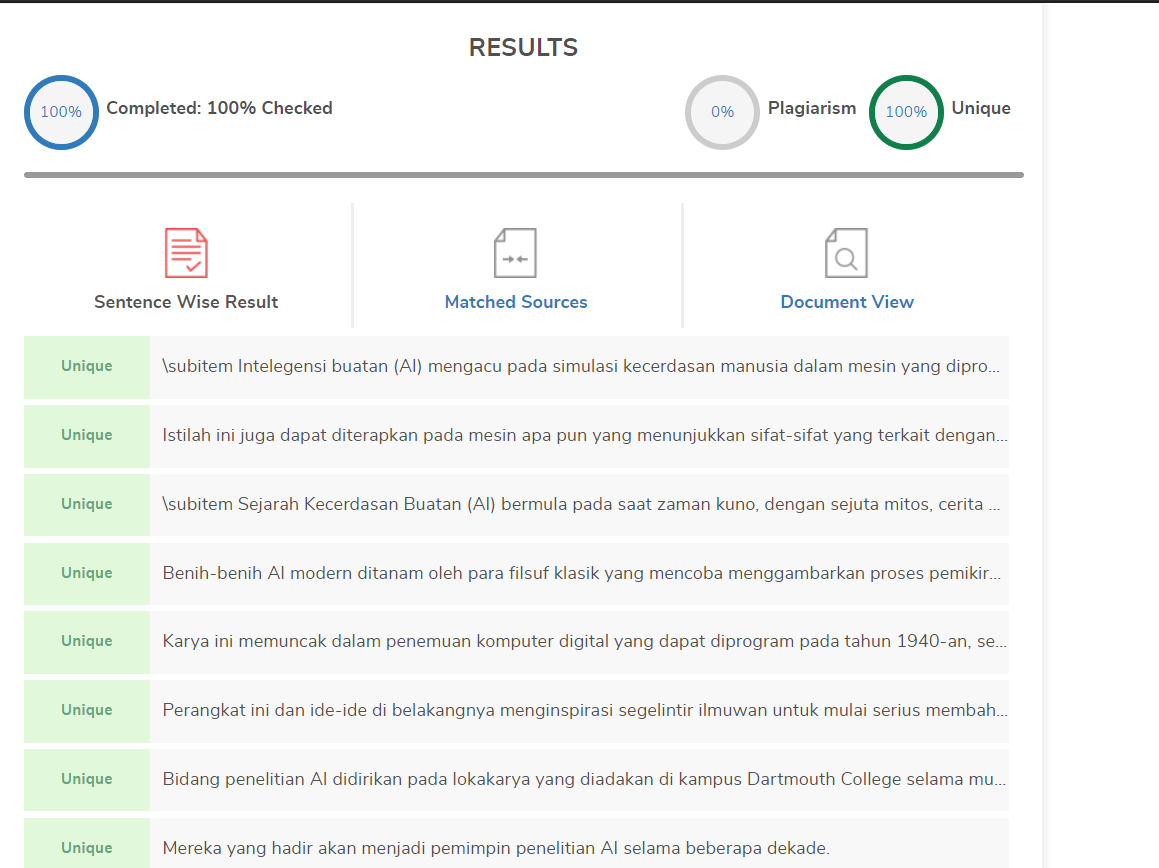
\includegraphics[scale=0.5]{figures/1174050/chapter1/plagiarism.png}
\caption{Plagiarism}
\end{figure}
\section{1174057 Alit Fajar Kurniawan}
\subsection{Teori}
	\subsubsection {Sejarah Perkembangan dan Definisi Artificial Intelligence}
	\par Kecerdasan buatan merupakan sebuah bidang dalam ilmu computer yang begitu penting di zaman ini dan masa yang akan datang guna mewujudkan sebuah sistem computer yang begitu cerdas. Artificial Intelligence atau biasa di singkat dengan AI berasal dari bahasa latin yang dimana intelligence berarti saya paham.
	\par Pada tahun 1955, Newell dan juga Simon telah mengembangkan The Logic Theorist, yaitu program AI pertama. Dimana program tersebut mempresentasikan sebuah masalah sebagai model pohon, lalu diselesaikan dengaan cara memilih cabang yang akan mewujudkan kesimpulan terbenar dan tepat. Program AI tersebut berdampak sangat besar dan dapat mendaji batu loncatan yang cukup penting dalam mengembangkan bidang AI \cite{baraja2008kecerdasan}.
	\par
	Masa Perkembangan AI dimulai pada awal era komputer elektronik pada tahun 1941. dimana ditemukannya alat penyimpanan dan pemrosesan informasi. kemudian dilanjutkan pada masa-masa persiapan AI yang terjadi pada tahun 1943-1956. Pada sekitaran tahun 1952-1969 merupakan masa awal perkembangan AI terjadi, dan pada tahun 1966-1974 perkembangan AI mengalami penurunan atau melambatnya proses dalam melakukan pengembangan. pada tahun 1969 sampai 10 tahun kedepan kembali terjadi perkembangan yang menciptakan inovasi sistem berbasis pengetahuan. dan sekitaran tahun 1980-an AI kembali menjadi sebuah industri yang terus berkembang sampai sekarang ini.


	\subsubsection{learning, klasifikasi, regresi dan unsupervised learning. Data set, training set dan testing set}
	\begin{enumerate}
	\item
	Definisi Supervised Learning Dan Unsupervised Learning
	\subitem
	Supervised Learning merupakan suatu pendekatan yang dimana terdapat data dan variable yang telah ditargetkan sehingga pendekatan tersebut bertujuan untuk dapat mengelompokkan sebuah data ke data yang sudah ada, beda dengan Unsupervised learning yang tidak mempunyai data, sehingga data yang ada harus di kelompokkan menjadi beberapa bagian.
	\item
	Definisi  Klasifikasi Dan Regresi
	\subitem
	Klasifikasi adalah sebuah kegiatan penggolongan atau pengelompokkan. Menurut kamus besar bahasa Indonesia yang dimana klasifikasi merupakan penyusunan sistem di dalam kelompok atau golongan berdasarkan kaidah atau standar yang telah ditetapkan. Regresi adalah sebuah metode analisis statistic yang akan digunakan untuk melihat pengaruh variable.
	\item
	Devinisi Dataset, Training Set, Dan Testing Set
	\subitem
	Dataset adalah sebuah objek yang akan mempresentasikan sebuah data dan relasinya di memory. Struktur pada dataset ini mirip dengan data yang ada di dalam database. Training set adalah bagian dari dataset yang berperan dalam membuat prediksi atau algoritma sesuai tujuan masing–masing. Testing set adalah bagian dari dataset yang akan di tes guna melihat keakuratatan atau ketepatan datanya.
	\end{enumerate}

\subsection{Praktek}
	\subsubsection{Instalasi}
	\begin{enumerate}
		\item Melakukan instalasi library scikit pada anaconda, ketik kan pip install -U scikit-learn pada terminal anaconda. 

		\begin{figure}[H]
		\centering
		\includegraphics[width=1\textwidth]{figures/1174057/chapter1/1.png}
		\caption{Instalasi Scikit Learn}
		\label{print}
		\end{figure}

		\item Setelah selesai instalasi, pilih salah satu example dari website Scikit. 
		\begin{figure}[H]
		\centering
		\includegraphics[width=1\textwidth]{figures/1174057/chapter1/2.png}
		\caption{Example}
		\label{print}
		\end{figure}

		\lstinputlisting[firstline=1, lastline=19]{src/1174057/chapter1/example.py}
		\par kemudian coba jalankan, lihat hasilnya
		\begin{figure}[H]
		\centering
		\includegraphics[width=1.5\textwidth]{figures/1174057/chapter1/3.png}
		\caption{Example}
		\label{print}
		\end{figure}

		\item latihan 2 Mencoba Loading an example dataset
		\lstinputlisting[firstline=1, lastline=9]{src/1174057/chapter1/dataset.py}
		\subitem hasil dari data digits
		\begin{figure}[H]
		\centering
		\includegraphics[width=1.5\textwidth]{figures/1174057/chapter1/4.png}
		\caption{Result Data Digits}
		\label{print}
		\end{figure}

		\subitem hasil dari digits.target
		\begin{figure}[H]
		\centering
		\includegraphics[width=1\textwidth]{figures/1174057/chapter1/5.png}
		\caption{Result digits.target}
		\label{print}
		\end{figure}

		\subitem hasil dari digits.image
		\begin{figure}[H]
		\centering
		\includegraphics[width=1\textwidth]{figures/1174057/chapter1/6.png}
		\caption{Result digits.image}
		\label{print}
		\end{figure}

		\item latihan 3 Mencoba Learning and predicting
		\lstinputlisting[firstline=1, lastline=9]{src/1174057/chapter1/learning.py}
		\par kemudian coba jalankan, lihat hasilnya
		\begin{figure}[H]
		\centering
		\includegraphics[width=1\textwidth]{figures/1174057/chapter1/7.png}
		\caption{Result Learning and predicting}
		\label{print}
		\end{figure}

		\item latihan 4 Mencoba Model persistence
		\lstinputlisting[firstline=1, lastline=16]{src/1174057/chapter1/modelpersistence.py}
		\par kemudian coba jalankan, lihat hasilnya
		\begin{figure}[H]
		\centering
		\includegraphics[width=1\textwidth]{figures/1174057/chapter1/8.png}
		\caption{Result Model persistence}
		\label{print}
		\end{figure}

		\item latihan 5 Mencoba Conventions
		\lstinputlisting[firstline=1, lastline=46]{src/1174057/chapter1/conventions.py}
		\par kemudian coba jalankan, lihat hasilnya
		\begin{figure}[H]
		\centering
		\includegraphics[width=1\textwidth]{figures/1174057/chapter1/9.png}
		\caption{Result Conventions}
		\label{print}
		\end{figure}

	\end{enumerate}

\subsection{Penanganan Error}
	\begin{enumerate}
		\item Screenshoot Error
		\begin{figure}[H]
		\centering
		\includegraphics[width=1\textwidth]{figures/1174057/chapter1/error1.png}
		\caption{Error}
		\label{print}
		\end{figure}

		\begin{figure}[H]
		\centering
		\includegraphics[width=1\textwidth]{figures/1174057/chapter1/error2.png}
		\caption{Error}
		\label{print}
		\end{figure}

		\item Tuliskan kode dan jenis error
			\subitem is not defined, xception yang terjadi saat syntax melakukan eksekusi terhadap local name atau global name yang tidak terdefinisi.
			\subitem invalid syntax

		\item Solusi penanganan error
			\subitem Solusinya adalah memastikan variabel atau function yang dipanggil ada atau tidak salah ketik. 
			\subitem Periksa kembali syntax yang dibuat, bisa saja ada kesalahan dalam spasi.
	\end{enumerate}

\subsection{Bukti Tidak Plagiat}
	\begin{figure}[H]
		\centering
		\includegraphics[width=1\textwidth]{figures/1174057/chapter1/plagiat.png}
		\caption{Plagiarisme}
		\label{print}
	\end{figure}
\section{1174039 - Liyana Majdah Rahma}
        \subsection{Teori}
            \subsubsection{Definisi Kecerdasan Buatan}

            Artificial Inteligence adalah kecerdasan yang ditambahkan  pada suatu sistem yang dapat diatur dalam konteks secara ilmiah. Menurut Michael Haelein menyatakan bahwa  AI meupakan “sistem yang mempunyai kemampuan untuk menguraikan, belajar agar dapat dugunakan untuk mencapai tujuan dengan melalui adaptasi yang fleksibel”. Kecerdasan buatan juga dapat dibuat dan dimasukkan ke dalam mesin agar dapat melakukan pekerjaan seperti yang dapat dilakukan manusia dengan cepat dan tepat. 
            
            \subsubsection{Sejarah Kecerdasan Buatan}

            Sejarah Kecerdasan buatan pertama kali terjadi pada zaman kuno, terdapat mitos ataupun cerita dan desas-desus tentang sebuah mahkluk yang mempunyai kecerdasan serta kesadaran yang diberikan oleh pengrajin. Benih - benih nya mulai ditanam oleh para filsuf klasik yang mencari cara untuk menggambarkan proses berfikir manusia sebagai manipulasi simbol secara mekanis yang memuncak pada penemuan komputer digital di tahun 1940-an, yaitu sebuah mesin yang didasarkan penalaran matematika. Istilah kecerdasan buatan sendiri baru muncul pada tahun 1956, dan teori -teori nya sudah muncul sejak tahun 1941. Dan Pada tahun 1973, sebagai tanggapan atas kritik dari James Lighthill dan tekanan terus-menerus dari kongres, AS dan Pemerintah Inggris menghentikan pendanaan penelitian yang tidak diarahkan pada kecerdasan buatan, dan tahun-tahun sulit berikutnya akan dikenal sebagai musim dingin AI. Tujuh tahun kemudian, sebuah inisiatif visioner oleh Pemerintah Jepang mengilhami pemerintah dan industri untuk menyediakan miliaran dolar dalam AI, tetapi pada akhir 80-an investor menjadi kecewa dengan kurangnya daya komputer (perangkat keras) yang dibutuhkan dan menarik lebih banyak dana.

            \subsubsection{Perkembangan Kecerdasan Buatan}
            \begin{enumerate}
                \item Pada tahun 1958, McCarthy di MIT AI Lab Memo orang pertama yang mendefinisikan bahasa pemrograman pada tingkat tinggi yaitu LISP, yang sekarang mendominasi pembuatan program-pogram kecerdasan buatan.
                \item Kemudian Pada tahun 1959, Nathaniel Rochester dari IBM serta mahasiswa-mahasiswanya mengeluarkan program kecerdasan buatan yaitu Geometry Theorm Prover. selain itu juga Program ini dapat mengeluarkan suatu teorema menggunakan aksioma-aksioma yang ada.
                \item Sistem Berbasis Pengetahuan pada tahun 1969-1979
                \item  Kecerdasan Buatan menjadi sebuah industri pada tahun 1980-1988. Kembalinya Jaringan Syaraf tiruan pada tahun 1986-sekarang.
            \end{enumerate}
        \subsection{Instalasi}
            \subsubsection{Instalasi Library Scikit dari Anaconda}
            \begin{enumerate}
                \item Download aplikasi Anaconda terlebih dahulu. 
                \item Install aplikasi Anaconda yang sudah di download tadi. 
                \item Simpan aplikasi sesuai folder yang kita pilih lalu next. 
                \item Centang Keduanya lalu tekan tombol install. 
                \item Setelah itu tunggu sampai proses instalasi selesai lalu jika sudah tekan tombol finish. 
                \item Lalu buka command prompt anda dan tuliskan perintah berikut ini untuk mengecek apakah aplikasinya sudah   terinstall. 
                \item Kemudian ketikkan perinta pip install -U scikit-learn seperti gambar berikut. 
            \end{enumerate}
<<<<<<< HEAD
			\begin{enumerate}
             \begin{figure}[H]
=======
            \begin{figure}[H]
>>>>>>> 8fcee3a95c7a660681b429f909ba80ac1a4fa418
                \includegraphics[width=4cm]{figures/1174039/chapter1/1.png}
                \centering
                \caption{Instalasi}
            \end{figure}
<<<<<<< HEAD
            \item Pilih salah satu example dari website tersebut lalu jalankan \hfill \break \lstinputlisting[firstline=1]{src/1174039/chapter1/no1.py}

                \item buka variable explolernya
                \begin{figure}[H]
                    \includegraphics[width=4cm]{figures/1174039/chapter1/2.png}
                    \centering
                    \caption{Variable Exploler}
                \end{figure}
			\end{enumerate}
=======
            \par salah satu example dari website tersebut lalu jalankan 
            \lstinputlisting[firstline=1, lastline=13]{src/1174039/chapter1/no1.py}
            \par buka variable explolernya
            \begin{figure}[H]
                \includegraphics[width=4cm]{figures/1174039/chapter1/2.png}
                \centering
                \caption{Variable Exploler}
            \end{figure}
>>>>>>> 8fcee3a95c7a660681b429f909ba80ac1a4fa418
            \subsubsection{Mencoba loading an example dataset}
            \begin{enumerate}
                \item mengambil data iris dan digit dari dataset \hfill \break \lstinputlisting[firstline=9, lastline=11]{src/1174039/chapter1/no2.py}
                
                \item Menampilkan data digits \hfill \break \lstinputlisting[firstline=13, lastline=13]{src/1174039/chapter1/no2.py}
                
                \begin{figure}[H]
                    \includegraphics[width=4cm]{figures/1174039/chapter1/3.png}
                    \centering
                    \caption{Data Digits}
                \end{figure}

                \item menampilkan digits.target
                \hfill \break \lstinputlisting[firstline=15, lastline=15]{src/1174039/chapter1/no2.py}

                \begin{figure}[H]
                    \includegraphics[width=4cm]{figures/1174039/chapter1/4.png}
                    \centering
                    \caption{Digits Target}
                \end{figure}

                \item menampilkan data bentuk 2D. \hfill \break \lstinputlisting[firstline=17, lastline=17]{src/1174039/chapter1/no2.py}

                \begin{figure}[H]
                    \includegraphics[width=4cm]{figures/1174039/chapter1/5.png}
                    \centering
                    \caption{Data 2D}
                \end{figure}
            \end{enumerate}

            \subsubsection{Mencoba Learning and Predicting}
            \hfill \break \lstinputlisting[firstline=1, lastline=12]{src/1174039/chapter1/no3.py}

            \subsubsection{Mencoba Model Presistence}
            \hfill \break \lstinputlisting[firstline=1, lastline=6]{src/1174039/chapter1/no4.py}

            \subsubsection{Mencoba Conventions}
            \hfill \break \lstinputlisting[firstline=1, lastline=7]{src/1174039/chapter1/no5.py}
        \subsection{Penanganan Error}
            \subsubsection{Screenshot Error}
            \begin{figure}[H]
                \includegraphics[width=4cm]{figures/1174039/chapter1/eror.png}
                \centering
                \caption{Data 2D}
            \end{figure}
            \subsubsection{Kode error dan jenis error}
            Jenis errornya adalah value error
            \hfill \break \lstinputlisting[firstline=15, lastline=15]{src/1174039/chapter1/no3.py}
            \subsubsection{Solusi Error}
            Solusinya adalah dengan menggantikan  nilai nya adalah n\_samples nya agar tidak 0
        \subsection{Cek Plagiarism}
            \begin{figure}[H]
                \includegraphics[width=4cm]{figures/1174039/chapter1/plagiat.png}
                \centering
                \caption{Cek Plagiarism}
            \end{figure}

\chapter{Chapter 2}
%\section{1174006 - Kadek Diva Krishna Murti}
Lorem ipsum dolor sit amet, consectetur adipiscing elit.

\lstinputlisting[firstline=1, lastline=8]{references.bib}
\hfill\break
\begin{figure}[H]
    \includegraphics[width=4cm]{kreatiflogo.png}
    \centering
    \caption{Kecerdasan Buatan.}
\end{figure}

\begin{enumerate}
	\item Lorem ipsum dolor sit amet, consectetur adipiscing elit.
	\item Lorem ipsum dolor sit amet, consectetur adipiscing elit.
	\item Lorem ipsum dolor sit amet, consectetur adipiscing elit.
\end{enumerate}

\subsection{Teori}

\subsection{Praktek}

\subsection{Penanganan Error}

\subsection{Bukti Tidak Plagiat}
\begin{figure}[H]
	\includegraphics[width=4cm]{kreatiflogo.png}
	\centering
	\caption{Kecerdasan Buatan.}
\end{figure}
\section{1174042 Faisal Najib Abdullah}

\subsection{Teori}
\begin{enumerate}
\item Jelaskan Apa Itu binari calssification dilengkapi ilustrasi gambar sendiri.\par
Binary Classification atau biominal adalah tugas mengklasifikasikan unsur usur dari himpunan yang diberikan kedalam kedua kelompok berdasarkan aturan klasifikasi yang telah ditetapkan. binari clasification juga dapat diartikan sebagai pembagi yang hanya memberikan dua pilihan contohnya benar dan salah atau klasifikasi tongkat panjang atau pendek. penjelasan lebih singkatnya binari classification merupakan kegiatam mengkelasifikasikan yang hanya memberikan dua class.
\begin{figure}[ht]
\centering
\includegraphics[scale=0.2]{figures/1174042/chapter2/1,1.jpeg}
\caption{contoh binari calssification}
\label{contoh}
\end{figure}


\item Jelaskan Apaitu supervised learning , unsupervised learning dan clusterring dengan ilustrasi gambar sendiri.\par
supervised learning adalah cara untuk mengklasifikasikan suatu objek atau data yang telah di tentukan kelas kelasnya contoh pada sayuran tumbuhan wortel termasuk yang mengandung vitamin A berarti tumbuhan wortel telah di kategorikan kedalam sayuran yang mengandung vitamin A. sedangkan kangkung mengandung zat besi yang berarti tumbuhan kangkung telah di kategorikan kedalam sayuran yang mengandung zat besi untuk lebih jelasnya dapat dilihat pada gambar.\par
\begin{figure}[ht]
\centering
\includegraphics[scale=0.2]{figures/1174042/chapter2/1,2.jpeg}
\caption{contoh supervised learning}
\label{contoh}
\end{figure}

unsupervised learning merupakan cara untuk mengklasifikasi tanpa adanya kelas untuk menentukan jenisnya contoh sayuran berarti semua objek yang memiliki ciri ciri sayuran di kategorikan kedalam sayuran untuk lebih jelasnya dapat dilihat pada gambar.\par
\begin{figure}[ht]
\centering
\includegraphics[scale=0.2]{figures/1174042/chapter2/1,3.jpeg}
\caption{contoh unsupervised learning}
\label{contoh}
\end{figure}

clustering merupakan peroses mengklasifikasikan yang berdasarkan suatu parameter dalam penentuannya contoh pada berat sayuran sayuran A memiliki berat 100 gr dan sayuran B memiliki berat 120 gr yang berarti berat sayuran dibagi dua parameter yaitu lebih kecil samadengan 100 gram dan lebih besar dari gram contoh pada gambar.\par
\begin{figure}[ht]
\centering
\includegraphics[scale=0.2]{figures/1174042/chapter2/1,4.jpeg}
\caption{contoh clusterring}
\label{contoh}
\end{figure}


\item Jelaskan apa itu evaluasi dan akurasi dan disertai ilustrasi contoh dengan gambar sendiri.\par
evaluasi adalah pengumpulan pengumpulan dan pengamatan dari berbagai macam bukti untuk mengukur dampak efektifitas dari suatu objek, program, atau proses berkaitan  dengan spesifikasi atau persyaratan yang telah di tetapkan sebelumnya. sedangkan akurasi itu sndiri merupakan bagian dari evaluasi yang merupakan ketepatan data terhadap suatu objek berdasarkan keriteria tertentu. kita dapat mengevaluasi seberapa baik model bekerja dengan mengukur akurasinya. ketepatan akan di definisikan sebagai presentase kasus yang di klasifikasikan dengan benar. hal ini berkaitan dengan confusion matrix pada materi selanjutnya. contoh evaluasi untuk membedakan burung dengan ayam terdapat parameter yaitu ukuran badan dan fungsi sayap pada hewan tersebut. lebih jelanya pada gambar berikut:
\begin{figure}[ht]
\centering
\includegraphics[scale=0.2]{figures/1174042/chapter2/1,5.jpeg}
\caption{contoh evaluasi dan akurasi}
\label{contoh}
\end{figure}


\item Jelaskan bagaimana cara membuat Confusion Matrix, Buat confusion matrix sendiri.\par
Dalam pembuatan confusion matrix tentukan parameter atau objek yang akan di evaluasi contoh bunga melati , bunga mawar, dan bunga kenangan buat tabel dengan baris dan kolom berjumlah tiga kemudian tentukan nilai miring pada setiap kolom tersebut disini saya memberi nilai 30 dengan ketentuan setiap baris harus berisi nilai 30 nilai tersebut jika terbagi ke kolom lain maka jumlahnya harus bernilai 30 jika tidak berarti data tersebut tidak akurat. untuk lebih jelanya dapat dilihat pada gambar berikut :
\begin{figure}[ht]
\centering
\includegraphics[scale=0.2]{figures/1174042/chapter2/1,6.jpeg}
\caption{contoh Confusion Matrix}
\label{contoh}
\end{figure}


\item Jelaskan bagaimana K-fold cross validation bekerja dengan gambar ilustrasi contoh buatan sendiri.
K-fold Cross Validation merupakan cara untuk melatih suatu mesin dimana di dalammya terdapat data set yang dibagi menjadi dua yaitu untuk data testing dan data training contoh 1000 data merupakan data set dan 200 data digunakan untuk data testing kemudian 800 datanya digunakan untuk data training dimana data training tersebut digunakan untuk menentukan nilai bobot yang dimasukan kedalam rumus regresi linier. sedangkan nilai testing akan dijadikan nili inputan untuk rumus regresi linier. contohnya dapat dilihat pada gambar berikut :
\begin{figure}[ht]
\centering
\includegraphics[scale=0.2]{figures/1174042/chapter2/1,7.jpeg}
\caption{contoh K-fold cross validation}
\label{contoh}
\end{figure}


\item Jelaskan Apa itu decision tree dengan gambar ilustrasi contoh buatan sendiri.\par
Decision tree (pohon keputusan) merupakan implementasi dari binari clasification dimana pada pohon keputusan akan terdapat root atau akar dan cabang cabangnya yang nilainya seperti if contoh pada root berisi nilai jenis kelamin, apakah perempuan pada cabang satu bernilai iya dan pada cabang dua bernilai tidak jika nilainya iya berarti jenis kelamminya perempuan dan jika tidak maka bernilai laki-laki.
agar lebih jelas dapat dilihat pada gambar decision tree berikut:
\begin{figure}[ht]
\centering
\includegraphics[scale=0.2]{figures/1174042/chapter2/1,8.jpeg}
\caption{contoh decision tree}
\label{contoh}
\end{figure}


\item jelaskan apa itu information gain dan entropi dengan gambar ilustrasi buatan sendiri.\par
informasion gain merupakan informasi atau keriteria dalam pembagian sebuah objek contoh information gain pada laki-laki yaitu berrambut lurus, mata belo, berkumis, berjenggot, dan memiliki jakun. untuk lebih jelasnya dapat dilihat pada gambar berikut :\par
\begin{figure}[ht]
\centering
\includegraphics[scale=0.2]{figures/1174042/chapter2/1,9.jpeg}
\caption{contoh information gain}
\label{contoh}
\end{figure}
sedangkan entropi merupakan ukuran keacakan dari informasi semakin tinggi entropi maka semakin sulit dalam menentukan keputusan contoh dalam menentukan jenis kelamin semakin detail informasi maka akan semakin susah dalam menentukan keputusan.
\end{enumerate}







\subsection{Sikic-Learn}
\begin{enumerate}
\item pada surcode pertama yang dapat dilihat pada gambar pada baris pertama di tuliskan yang berarti mengimport library padas. selanjutnya pada baris ke dua codingan tersebut berisi pada code tersebut terdapat variabel muaraenim yang berisi inisialisasi padas dengan aksi untuk membaca vfile csv yang terdapat pada direktori pada komputer kemudian terdapat sep samadengan titik koma yang berarti pemisah field di dalam vile tersebut merupakan titik koma. kemudian pada bagian akhir terdapat code len (nama variabel) yang berarti akan menghotung jumlah baris pada file tersebut.
\lstinputlisting{src/1174042/chapter2/2,1.py}
\begin{figure}[ht]
\centering
\includegraphics[scale=0.5]{figures/1174042/chapter2/2,1.JPG}
\caption{hasil}
\label{contoh}
\end{figure}

\item Pada code selanjutnya akan ditambahkan fungsi untuk lulus atau gagal yang dibuat berupa kolom kolom yang di dalammya terdapat nilai 0 dan 1 dimana 0 berarti gagal dan 1 berarti lulus. kemudian variabel pada codingan sebelumnya masih digunakan. dimana variabel muaraenim digunakan karena berisi nilai file csv kemudian dilakukan ekseskusi dengan parameter G1, G2, dan G3 dengan fungsi lambda yang berarti if bersarang atau if didalam if yang berarti nilai yang di eksekusi akan dilempar ke dalam setiap paramater sasuai dengan kriteria dan axis=1 yaitu nilai tersebut akan digunakan dari tiap baris data. sedangkan pada codingan selanjutnya variabel muaraenim di berikan aksi drop yaitu penurunan nilai pada bagian baris data. dan pada code muaraenim.head () yaitu untuk mengeksekusi codingan sebelumnya.
\lstinputlisting{src/1174042/chapter2/2,2.py}
\begin{figure}[ht]
\centering
\includegraphics[scale=0.5]{figures/1174042/chapter2/2,2.JPG}
\caption{hasil}
\label{contoh}
\end{figure}

\item pada kodingan selanjutnya diguanakn untuk menambahkan nilai numerik berupa 0 dan 1 yang dirubah dari nilai tidak dan iya hal ini merupakan fungsi dari codingan get\_dummies pada baris pertama yang nilainya diambil dari variabel muaraenim yang telah di dekralasikan tadi banyaknya data numerik itu sendiri tergantung pada field dari kolom yang di camtumkan pada codingan dengan catatan field tersebut harus ada dalam data csv yang di import oleh codingan pertama tadi maka hasilnya akam merubah data dalam field tersebut menjadi 0 dan 1.
\lstinputlisting{src/1174042/chapter2/2,3.py}
\begin{figure}[ht]
\centering
\includegraphics[scale=0.5]{figures/1174042/chapter2/2,3.JPG}
\caption{hasil}
\label{contoh}
\end{figure}

\item selanjutnya pada codingan selanjutnya yaitu menentukan data training dan data testing dari dataset dimana variabel muaraenim yang berisi data csv tadi dibuat perbandingan 500 untuk data training dan sisanya yaitu 149 digunakan untuk data testing hal ini di lakukan pada baris ke 1 sampai ke 3 pada gambar kemudian nilai tersebut di turunkan  brdasarkan baris pada data set hal itu dapat dilihat pada baris ke 4 sampai ke 9 pada gambar kemudian selanjutnya mengimport library numpy yang berguna untuk oprasi vektor dan matrix karna data diatas berupa data matrix maka library ini di gunakan.
\lstinputlisting{src/1174042/chapter2/2,4.py}
\begin{figure}[ht]
\centering
\includegraphics[scale=0.5]{figures/1174042/chapter2/2,4.JPG}
\caption{hasil}
\label{contoh}
\end{figure}

\item selanjutnya yaitu membuat pohon keputusan pada baris pertama yairu memasukan librari tree kemudian pada baris kedua dibuat variabel palembang dengan nilai DecisionTreeClasifier yang merupakan paket atau fungsi dari scikit-learn yang merupakan class yang mampu melakukan multi class. sedangkan max\_depth=5 merupakan untuk penyesuaian data terhadap pohon keputusan itu sndiri.
\lstinputlisting{src/1174042/chapter2/2,5.py}
\begin{figure}[ht]
\centering
\includegraphics[scale=0.5]{figures/1174042/chapter2/2,5.JPG}
\caption{hasil}
\label{contoh}
\end{figure}

\item selanjutnya yaitu pembuatan gambar dari pohon keputusan yang tadi di buta pada codingan sebelumnya pada baris pertama codingan ya itu mengimport library graphviz kemudian pada baris ke dua yaitu pemberian nilai pada variabel baru dot data nilainy diambil dari pembuatan puhon keputusan tadi kemudian di tentukannya nilai benar dan salah dari codingan tersebut setelah itu dibuatlah sebuah variabel untuk menampung hasil eksekusi tersebut kemudian variabel tersebut di running.
\lstinputlisting{src/1174042/chapter2/2,6.py}
\begin{figure}[ht]
\centering
\includegraphics[scale=0.5]{figures/1174042/chapter2/2,6.JPG}
\caption{hasil}
\label{contoh}
\end{figure}

\item selanjutnya pembuatasn method untuk menyimpan data pohon dengan menarik data langsung dari pohon keputusan.
\lstinputlisting{src/1174042/chapter2/2,7.py}
\begin{figure}[ht]
\centering
\includegraphics[scale=0.5]{figures/1174042/chapter2/2,7.JPG}
\caption{hasil}
\label{contoh}
\end{figure}

\item selanjutnya pada codingan berikut yaitu digunakan untuk mencetak nilai score rata-rata dari ketepatan data yang telah di olah.
\lstinputlisting{src/1174042/chapter2/2,8.py}

\item selanjutnya yaitu digunakan untuk memeriksa akurasi dari ketepatan hasil pengolahan data tersebut maka akan didapat nilai rata-rata 60 persen dari hasil pengolahan data tersebut, pada codingan tersebut pada baris ke satu melakukan import library dari sklern kemudian pada baris selanjutnya mengisi nilai skor dengan nilai pada variabel palembang setelah hal tersebut dilakukan kemudian data tersebut di eksekusi.
\lstinputlisting{src/1174042/chapter2/2,9.py}
\begin{figure}[ht]
\centering
\includegraphics[scale=0.5]{figures/1174042/chapter2/2,9.JPG}
\caption{hasil}
\label{contoh}
\end{figure}

\item membuat rank akurasi dari 1 sampai 100 untuk melihat akurasi data apakah datatersebut terdapat di rata rata 60 persen atau tidak dengan cara membuat lagi variabel baru dengan nilai tree diadalammya jadi hampir mirip seperti membuat pohon keputusan namun ini langsung dalam bentuk rata rata akurasi yanlebih spesifik.
\lstinputlisting{src/1174042/chapter2/2,10.py}
\begin{figure}[ht]
\centering
\includegraphics[scale=0.5]{figures/1174042/chapter2/2,10.JPG}
\caption{hasil}
\label{contoh}
\end{figure}

\item untuk selanjutnya yaitu menentukan nilai untuk grafik hampirsama dengan nilia akurasi tadi pertama tentukan rank atai batasan nilai itu disini batasannya di mulai dari 1 sampai 20 dengan menggunakan nilai tree tadi maka hasilnya dapat ditentuka kemudian buat variabel i untuk penomoran tiap record yang keluar atau recod hadil dari eksekusi tree tersebut.
\lstinputlisting{src/1174042/chapter2/2,11.py}
\begin{figure}[ht]
\centering
\includegraphics[scale=0.5]{figures/1174042/chapter2/2,11.JPG}
\caption{hasil}
\label{contoh}
\end{figure}

\item terakhir yaitu pembuatan grafik untuk pembuatan grafik diambil data dari codingan sebelumnya yang 20 record tadi dengan cara mengimport libray matplotlib.pyplot yang di inisialisasi menjadi bakwankemudian inisialisasi tersebut di eksekusi.
\lstinputlisting{src/1174042/chapter2/2,12.py}
\begin{figure}[ht]
\centering
\includegraphics[scale=0.5]{figures/1174042/chapter2/2,12.JPG}
\caption{hasil}
\label{contoh}
\end{figure}
\end{enumerate}

\subsection{Penanganan Error}
\begin{enumerate}
\item skrinsut error
\begin{figure}[ht]
\centering
\includegraphics[scale=0.5]{figures/1174042/chapter2/error.JPG}
\caption{Error}
\label{contoh}
\end{figure}

\item kode error dan jenis errornya .
\begin{verbatim}
import graphviz
dot_data = tree.export_graphviz(palembang, out_file=None, label="all", impurity=False, proportion=True,
                                feature_names=list(muaraenim_train_att), class_names=["fail", "pass"], 
                                filled=True, rounded=True)
graph = graphviz.Source(dot_data)
graph
\end{verbatim}

pada codingan tersebut error karena graphiznya belu di istall 

\item Solusi pemecahan masalah \par
buka CMD komputer anda run as administrator koemudian masukan perintah conda install graphviz.
\end{enumerate}


\subsection{Plagiat}
\begin{figure}[ht]
\centering
\includegraphics[scale=0.5]{figures/1174042/chapter2/plagiat.jpg}
\caption{Error}
\label{contoh}
\end{figure}

\section{1174035 Luthfi Muhammad Nabil}

\subsection{Teori}
\begin{enumerate}
\item Jelaskan Apa Itu Binary Classification dilengkapi ilustrasi gambar sendiri.\par
Binary Classification adalah sebuah metode untuk menklasifikasikan elemen yang dibentuk seperti grup untuk dibagi menjadi 2 grup. Dari 2 grup tersebut diprediksikan setiap anggota pada grup yang mana sesuai dengan yang diatur pada aturan klasifikasi. Data atau konteks yang didapat membutuhkan keputusan dari item tersebut memiliki properti kualitatif, karakteristik yang spesifik, atau tipikal klasifikasi biner.
\begin{figure}[H]
\centering
\includegraphics[scale=0.2]{figures/1174035/chapter2/binary_classification.jpeg}
\caption{contoh binary classification}
\label{contoh}
\end{figure}


\item Jelaskan Apa itu supervised learning , unsupervised learning dan clusterring dengan ilustrasi gambar sendiri.\par
Supervised learning adalah kondisi yang menggunakan variabel input dan output untuk dapat dilakukan pemetaan input output yang sudah didapat. Disebud Supervised Learning karena proses dari pembelajaran algoritma dari pembelajan yang disumberkan dengan dataset dapat dipikirkan seperti seorang guru yang mengawasi proses pembelajaran. Proses pembelajaran dari algoritma akan berhenti saat algoritma sudah mendapatkan level dari performansi yang dapat diterima. \par
Unsupervised learning adalah kondisi dimana kamu hanya memiliki input data tanpa memiliki variabel output yang sesuai. Tujuan dari unsupervised learning adalah untuk memodelkan distribusi pada data untuk mengetahui lebih lanjut mengenai data. Disebut unsupervised learning karena pada metode ini, tidak ada jawaban yang tepat dan tidak ada pengarah. Sehingga algoritma akan ditinggalkan sesuai rancangan demi menemukan dan dapat mengolah data yang menarik pada saat yang akan datang. \par
Clustering adalah sebuah metode untuk membedakan data - data menjadi kumpulan dari group yang isinya merupakan data yang serupa setiap grupnya. Basisnya dapat berupa kesamaan atau perbedaan dari setiap grup tersebut. \par
\begin{figure}[H]
\centering
\includegraphics[scale=0.2]{figures/1174035/chapter2/clustering.jpeg}
\caption{contoh clustering}
\label{contoh}
\end{figure}


\item Jelaskan apa itu evaluasi dan akurasi dan disertai ilustrasi contoh dengan gambar sendiri.\par
Evaluasi adalah kegiatan yang dilakukan untuk menentukan sebuah nilai yang dapat diambil dari suatu hal. Beberapa contoh evaluasi diantaranya menilai sebuah barang, bahaya dari penyakit, dan lain sebagainya dengan parameter yang digunakan yaitu mengetahui faktor - faktor yang menyebabkan atau akibat yang akan terjadi jika dibiarkan. 

\item Jelaskan bagaimana cara membuat Confusion Matrix, Buat confusion matrix sendiri.\par
Confusion Matrix merupakan metode untuk menghitung akurasi pada data mining atau Sistem Pendukung Keputusan. Untuk menggunakan Confusion Matrix, ada 4 istilah sebagai hasil proses dari klasifikasi. Diantaranya adalah :

\begin{itemize}
    \item True Positive : Data positif yang terdeteksi memiliki hasil benar
    \item False Positive : Data Positif yang terdeteksi memiliki hasil salah
    \item True Negative : Data negatif yang terdeteksi memiliki hasil benar
    \item False Negative : Data negatif yang terdeteksi memiliki hasil salah
\end{itemize}


\item Jelaskan bagaimana K-fold cross validation bekerja dengan gambar ilustrasi contoh buatan sendiri.
k-Fold Cross-Validation merupakan prosedur untuk mengambil sampel ulang yang digunakan untuk mengevaluasi sebuah "machine learning" model pada sampel data yang terbatas. Procedure yang ada memiliki satu parameter yang dipanggil k yang mengacu pada jumlah grup yang memberikan data sampel untuk dipisahkan.
K-fold Cross-validation akan melakukan hal berikut : 
\begin{enumerate}
    \item Mengacak dataset secara random
    \item Memisahkan dataset menjadi k group
    \item Untuk setiap grup, akan disesuaikan dan dievaluasikan
    \item Merekaphasil dari evaluasi dan penyesuaian menggunakan sampel dari model evaluasi
\end{enumerate}
\begin{figure}[H]
\centering
\includegraphics[scale=0.2]{figures/1174035/chapter2/kcode.jpeg}
\caption{contoh K-fold cross validation}
\label{contoh}
\end{figure}


\item Jelaskan Apa itu decision tree disertakan gambar ilustrasi contoh buatan sendiri.\par
Decision Tree merupakan sebuah struktur yang menentukan keputusan dan setiap konsekuensinya. Hasil dari setiap struktur biasanya menggunakan jawaban (True dan False) atau cabang lain yang akan menjadi pohon selanjutnya. Setiap keputusan diantaranya akan membandingkan kondisi yang diberikan kepada struktur untuk dibandingkan kondisi apa saja yang sudah didapat pada sistem tersebut. 


\item jelaskan apa itu information gain dan entropi dengan gambar ilustrasi buatan sendiri.\par
Information Gain merupakan total data yang didapat dari data - data acak yang data tersebut akan digunakan untuk analisis data lainnya. Information Gain ini digunakan pada decision tree sebagai label setiap aksi - aksi yang perlu dinilai validasinya. 
\begin{figure}[H]
\centering
\includegraphics[scale=0.2]{figures/1174035/chapter2/info_gain.jpeg}
\caption{contoh information gain}
\label{contoh}
\end{figure}
Entropi merupakan pengukuran sebuah data dan validnya data tersebut untuk dapat digunakan sebagai informasi yang akan dimasukkan ke Information Gain. Entropi menilai sebuah obyek berdasarkan kebutuhan di dunia nyata dan pengaruh pada sistem yang akan digunakan
\begin{figure}[H]
    \centering
    \includegraphics[scale=0.2]{figures/1174035/chapter2/entropi.jpeg}
    \caption{contoh information gain}
    \label{contoh}
    \end{figure}
\end{enumerate}

\subsection{Scikit-Learn}
\begin{enumerate}
    \item \hfill \break \lstinputlisting[firstline=11, lastline=13]{src/1174035/chapter2/sample1.py}
	\begin{figure}[H]
		\includegraphics[width=4cm]{figures/1174035/chapter2/1.png}
		\centering
		\caption{Hasil Percobaan 1}
    \end{figure}
    \item \hfill \break \lstinputlisting[firstline=15, lastline=17]{src/1174035/chapter2/sample1.py}
	\begin{figure}[H]
		\includegraphics[width=4cm]{figures/1174035/chapter2/2.png}
		\centering
		\caption{Hasil Percobaan 2}
    \end{figure}
    \item \hfill \break \lstinputlisting[firstline=19, lastline=20]{src/1174035/chapter2/sample1.py}
	\begin{figure}[H]
		\includegraphics[width=4cm]{figures/1174035/chapter2/3.png}
		\centering
		\caption{Hasil Percobaan 3}
    \end{figure}
    \item \hfill \break \lstinputlisting[firstline=22, lastline=35]{src/1174035/chapter2/sample1.py}
	\begin{figure}[H]
		\includegraphics[width=4cm]{figures/1174035/chapter2/4.png}
		\centering
		\caption{Hasil Percobaan 4}
    \end{figure}
    \item \hfill \break \lstinputlisting[firstline=37, lastline=39]{src/1174035/chapter2/sample1.py}
	\begin{figure}[H]
		\includegraphics[width=4cm]{figures/1174035/chapter2/5.png}
		\centering
		\caption{Hasil Percobaan 5}
    \end{figure}
    \item \hfill \break \lstinputlisting[firstline=41, lastline=44]{src/1174035/chapter2/sample1.py}
	\begin{figure}[H]
		\includegraphics[width=4cm]{figures/1174035/chapter2/6.png}
		\centering
		\caption{Hasil Percobaan 6}
    \end{figure}
    \item \hfill \break \lstinputlisting[firstline=46, lastline=46]{src/1174035/chapter2/sample1.py}
	\begin{figure}[H]
		\includegraphics[width=4cm]{figures/1174035/chapter2/7.png}
		\centering
		\caption{Hasil Percobaan 7}
    \end{figure}
    \item \hfill \break \lstinputlisting[firstline=48, lastline=48]{src/1174035/chapter2/sample1.py}
	\begin{figure}[H]
		\includegraphics[width=4cm]{figures/1174035/chapter2/8.png}
		\centering
		\caption{Hasil Percobaan 8}
    \end{figure}
    \item \hfill \break \lstinputlisting[firstline=50, lastline=54]{src/1174035/chapter2/sample1.py}
	\begin{figure}[H]
		\includegraphics[width=4cm]{figures/1174035/chapter2/9.png}
		\centering
		\caption{Hasil Percobaan 9}
    \end{figure}
    \item \hfill \break \lstinputlisting[firstline=56, lastline=59]{src/1174035/chapter2/sample1.py}
	\begin{figure}[H]
		\includegraphics[width=4cm]{figures/1174035/chapter2/10.png}
		\centering
		\caption{Hasil Percobaan 10}
    \end{figure}
    \item \hfill \break \lstinputlisting[firstline=61, lastline=70]{src/1174035/chapter2/sample1.py}
	\begin{figure}[H]
		\includegraphics[width=4cm]{figures/1174035/chapter2/11.png}
		\centering
		\caption{Hasil Percobaan 11}
    \end{figure}
    \item \hfill \break \lstinputlisting[firstline=72, lastline=75]{src/1174035/chapter2/sample1.py}
	\begin{figure}[H]
		\includegraphics[width=4cm]{figures/1174035/chapter2/12.png}
		\centering
		\caption{Hasil Percobaan 12}
	\end{figure}
\end{enumerate}
\subsection{Skrinsut Error}
Error yang didapat yaitu mengalami error tidak ada library graphviz yang terdeteksi
\begin{figure}[H]
    \includegraphics[width=4cm]{figures/1174035/chapter2/error.png}
    \centering
    \caption{Error}
\end{figure}
\subsection{Penanganan Error}
Solusinya adalah dengan menginstall library graphviz yang ada
\begin{figure}[H]
    \includegraphics[width=4cm]{figures/1174035/chapter2/error.png}
    \centering
    \caption{Error}
\end{figure}
\subsection{Plagiarisme}
\begin{figure}[H]
    \includegraphics[width=4cm]{figures/1174035/chapter2/plagiarism.png}
    \centering
    \caption{Hasil Pengecekan Plagiarisme}
\end{figure}

\section{1174057 Alit Fajar Kurniawan}
\subsection{Teori}
	\subsubsection{Jelaskan apa itu binary classification dilengkapi ilustrasi gambar sendiri}
	\par Binary classification merupakan jenis masalah pembelajaran mesin yang paling sederhana.
	mengkalrifikasikan elemen-elemen dari himpunan yang diberikan kedalam dua kelompok berdasarkan aturan klarifikasi. Contoh yang paling sederhana dalam binary classification yaitu mendeteksi dan mendiagnosa. Berikut contoh gambar Binary Classification, gambar 2.1
		\begin{figure}[H]
			\centering
			\includegraphics[width=0.5\textwidth]{figures/1174057/chapter2/1.jpg}
			\caption{Klasifikasi Binari}
			\label{print}
		\end{figure}

	\subsubsection{Jelaskan apa itu supervised learning dan unsupervised learning dan clustering dengan ilustrasi gambar sendiri}
	\par Supervised Learning merupakan paradigma belajar yang berkaitan dengan studi tentang bagaimana
	komputer dan sistem alami seperti manusia belajar \cite{zhou2018brief}. Tujuannya untuk menyimpulkan pemetaan fungsional berdasarkan serangkaian pelatihan atau mengelompokkan suatu data ke data yang sudah ada. Berikut contoh gambar Supervised Learning
		%\begin{figure}[H]
		%	\centering
		%	\includegraphics[width=1\textwidth]{figures/1174057/chapter2/2.png}
		%	\caption{Supervised Learning}
		%	\label{print}
		%\end{figure}
	\par Unsupervised Learning merupakan sebuah data yang belum ditentukan variabelnya jadi hanya berupa data saja. Dalam sebuah kasus Unsupervised Learning adalah aggap saja anda belum pernah membeli buku sama sekali dan pada suatu hari anda telah membeli buku dengan sangat banyak dalam kategori yang berbeda. Sehingga buku tersebut belum di kategorikan dan hanya berupa data buku saja.
		%\begin{figure}[H]
		%	\centering
		%	\includegraphics[width=1\textwidth]{figures/1174057/chapter2/3.png}
		%	\caption{Supervised Learning}
		%	\label{print}
		%\end{figure}
	\par Clustering merupakan metode pengelompokan data, clustering juga suatu proses partisi satu set objek data ke dalam himpunan bagian yang disebut dengan cluster. Objek yang pada cluster memiliki kesamaan secara karakteristik antara satu sama lainnya dan berbeda dengan cluster yang lain.
		%\begin{figure}[H]
		%	\centering
		%	\includegraphics[width=1\textwidth]{figures/1174057/chapter2/4.png}
		%	\caption{Supervised Learning}
		%	\label{print}
		%\end{figure}

\subsection{Praktek}

\subsection{Penanganan Error}

\subsection{Bukti Tidak Plagiat}
		\begin{figure}[H]
			\centering
			\includegraphics[width=1\textwidth]{figures/1174057/chapter2/plagiat.png}
			\caption{Plagiarisme}
			\label{print}
		\end{figure}



\section{1174050 Dika Sukma Pradana}

\subsection{Teori}
\begin{enumerate}
\item Jelaskan Apa Itu binari calssification dilengkapi ilustrasi gambar sendiri.\par
Klasifikasi biner atau binomial adalah tugas untuk mengklasifikasikan elemen-elemen dari himpunan tertentu ke dalam dua kelompok (memprediksi kelompok mana yang masing-masing dimiliki) berdasarkan aturan klasifikasi.
\begin{figure}[ht]
\centering
\includegraphics[scale=0.01]{figures/1174050/chapter2/1.jpg}
\caption{contoh binari calssification}
\label{contoh}
\end{figure}


\item Jelaskan Apaitu supervised learning , unsupervised learning dan clusterring dengan ilustrasi gambar sendiri.\par
sSupervised learning adalah sebuah metode pendekatan yang mana sudah terdapat data yang dilatiih, dan terdapat variabel yang ditargetkan atau yang menjadi tujuan sehingga tujuan dari pendekatan ini adalah mengkelompokan suatu data ke data yang sudah ada.  contoh pada nasi termasuk yang mengandung karbohidrat berarti nasi telah di kategorikan kedalam karbohidrat. sedangkan ayam mengandung protein yang berarti ayam telah di kategorikan  yang mengandung protein untuk lebih jelasnya dapat dilihat pada gambar.\par
\begin{figure}[ht]
\centering
\includegraphics[scale=0.01]{figures/1174050/chapter2/2.jpg}
\caption{contoh supervised learning}
\label{contoh}
\end{figure}

Sedangkan unsupervised learrning tidak memiliki data latiih, sehinggga dari data yang ada, kita mengelompokan data tersebbut menjadi dua bagian atau bahkan tiga bagian dan seterusnya.contoh ayam di kategorikan kedalam karbohidrat untuk lebih jelasnya dapat dilihat pada gambar.\par
\begin{figure}[ht]
\centering
\includegraphics[scale=0.01]{figures/1174050/chapter2/3.jpg}
\caption{contoh unsupervised learning}
\label{contoh}
\end{figure}

clustering merupakan peroses mengklasifikasikan yang berdasarkan suatu parameter dalam penentuannya contoh pada berat protein memiliki berat 1000 gr dan karbohidrat memiliki berat 1200 gr yang berarti berat dibagi dua parameter yaitu lebih kecil samadengan 1000 gram dan lebih besar dari 1000gram contoh pada gambar.\par
\begin{figure}[ht]
\centering
\includegraphics[scale=0.01]{figures/1174050/chapter2/4.jpg}
\caption{contoh clusterring}
\label{contoh}
\end{figure}


\item Jelaskan apa itu evaluasi dan akurasi dan disertai ilustrasi contoh dengan gambar sendiri.\par
evaluasi adalah pengumpulan pengumpulan dan pengamatan dari berbagai macam bukti untuk mengukur dampak efektifitas dari suatu objek, program, atau proses berkaitan  dengan spesifikasi atau persyaratan yang telah di tetapkan sebelumnya. sedangkan akurasi itu sndiri merupakan bagian dari evaluasi yang merupakan ketepatan data terhadap suatu objek berdasarkan keriteria tertentu. kita dappat mengevalluasi seberappa baik modell bekerja denggan menggukur akurasiinya. ketepatan akan di definisikan sebagai presentase kasus yang di klasifikasikan dengan benar. hal ini berkaitan dengan confusion matrix pada materi selanjutnya. contoh evaluasi untuk membedakan angsa dengan entok terdapat parameter yaitu panjang leher dan fungsi sifat dari hewan tersebut. lebih jelanya pada gambar berikut:
\begin{figure}[ht]
\centering
\includegraphics[scale=0.01]{figures/1174050/chapter2/5.jpg}
\caption{contoh evaluasi dan akurasi}
\label{contoh}
\end{figure}


\item Jelaskan bagaimana cara membuat Confusion Matrix, Buat confusion matrix sendiri.\par
Dalam pembuatan confusion matrix tentukan parameter atau objek yang akan di evaluasi contoh angsa,entok, bebek buat tabel dengan baris dan kolom berjumlah tiga kemudian tentukan nilai miring pada setiap kolom tersebut disini saya memberi nilai 15 dengan ketentuan setiap baris harus berisi nilai 15 nilai tersebut jika terbagi ke kolom lain maka jumlahnya harus bernilai 15 jika tidak berarti data tersebut tidak akurat. untuk lebih jelanya dapat dilihat pada gambar berikut :
\begin{figure}[ht]
\centering
\includegraphics[scale=0.01]{figures/1174050/chapter2/6.jpg}
\caption{contoh Confusion Matrix}
\label{contoh}
\end{figure}


\item Jelaskan bagaimana K-fold cross validation bekerja dengan gambar ilustrasi contoh buatan sendiri.
K-fold Cross Validation merupakan cara untuk melatih suatu mesin dimana di dalammya terdapat data set yang dibagi menjadi dua yaitu untuk data testing dan data training contoh 1000 data merupakan data set dan 300 data digunakan untuk data testing kemudian 700 datanya digunakan untuk data training dimana data training tersebut digunakan untuk menentukan nilai bobot yang dimasukan kedalam rumus regresi linier. sedangkan nilai testing akan dijadikan nili inputan untuk rumus regresi linier. contohnya dapat dilihat pada gambar berikut :
\begin{figure}[ht]
\centering
\includegraphics[scale=0.01]{figures/1174050/chapter2/7.jpg}
\caption{contoh K-fold cross validation}
\label{contoh}
\end{figure}


\item Jelaskan Apa itu decision tree dengan gambar ilustrasi contoh buatan sendiri.\par
Decision tree merupakan implementasi dari binari clasification dimana pada pohon keputusan akan terdapat root atau akar dan cabang cabangnya yang nilainya seperti if contoh pada root berisi nilai warna mawar, apakah merah pada cabang satu bernilai iya dan pada cabang dua bernilai tidak jika nilainya iya berarti mawar dan jika tidak maka bukan mawar.
agar lebih jelas dapat dilihat pada gambar decision tree berikut:
\begin{figure}[ht]
\centering
\includegraphics[scale=0.01]{figures/1174050/chapter2/8.jpg}
\caption{contoh decision tree}
\label{contoh}
\end{figure}


\item jelaskan apa itu information gain dan entropi dengan gambar ilustrasi buatan sendiri.\par
informasion gain merupakan informasi atau keriteria dalam pembagian sebuah objek contoh information gain pada llama yaitu leher panjang, ekor panjang, berkaki 4, buas, karnivora. untuk lebih jelasnya dapat dilihat pada gambar berikut :\par
\begin{figure}[ht]
\centering
\includegraphics[scale=0.01]{figures/1174050/chapter2/9.jpg}
\caption{contoh information gain}
\label{contoh}
\end{figure}
sedangkan entropi merupakan ukuran keacakan dari informasi semakin tinggi entropi maka semakin sulit dalam menentukan keputusan contoh dalam menentukan satu gen semakin detail informasi maka akan semakin susah dalam menentukan keputusan.
\end{enumerate}







\subsection{Sikic-Learn}
\begin{enumerate}
\item pada surcode pertama yang dapat dilihat pada gambar  pada baris pertama di tuliskan import pandas as baso yang berarti mengimport library padas. selanjutnya pada baris ke dua codingan tersebut berisi code tersebut terdapat variabel pecel yang berisi inisialisasi pandas dengan aksi untuk membaca vfile csv yang terdapat pada direktori pada komputer kemudian terdapat sep samadengan titik koma yang berarti pemisah field di dalam file tersebut merupakan titik koma. kemudian pada bagian akhir terdapat code len (nama variabel) yang berarti akan menghotung jumlah baris pada file tersebut. untuk hasilnya dapat dilihat pada gambar dibawah.
\lstinputlisting{src/1174050/chapter2/1.py}
\begin{figure}[ht]
\centering
\includegraphics[scale=0.5]{figures/1174050/chapter2/10.PNG}
\caption{hasil}
\label{contoh}
\end{figure}

\item Pada code selanjutnya akan ditambahkan fungsi untuk lulus atau gagal yang dibuat berupa kolom kolom yang di dalammya terdapat nilai 0 dan 1 dimana 0 berarti gagal dan 1 berarti lulus. kemudian variabel pada codingan sebelumnya masih digunakan. dimana variabel pecel digunakan karena berisi nilai file csv kemudian dilakukan ekseskusi dengan parameter G1, G2, dan G3 dengan fungsi lambda yang berarti if bersarang atau if didalam if yang berarti nilai yang di eksekusi akan dilempar ke dalam setiap paramater sasuai dengan kriteria dan axis=1 yaitu nilai tersebut akan digunakan dari tiap baris data. sedangkan pada codingan variabel pecel di berikan aksi drop yaitu penurunan nilai pada bagian baris data. dan pada code pecel.head yaitu untuk mengeksekusi codingan sebelumnya untuk lebih jelasnya dapat dilihat pada gambar dan hasilnya seperti pada gambar berikut :
\lstinputlisting{src/1174050/chapter2/2.py}
\begin{figure}[ht]
\centering
\includegraphics[scale=0.5]{figures/1174050/chapter2/11.PNG}
\caption{hasil}
\label{contoh}
\end{figure}

\item pada kodingan selanjutnya diguanakn untuk menambahkan nilai numerik berupa 0 dan 1 yang dirubah dari nilai tidak dan iya hal ini merupakan fungsi dari codingan get\_dummies pada baris pertama pada gambar yang nilainya diambil dari variabel pecel yang telah di dekralasikan tadi banyaknya data numerik itu sendiri tergantung pada field dari kolom yang di camtumkan pada codingan dengan catatan field tersebut harus ada dalam data csv yang di import oleh codingan pertama tadi maka hasilnya akam merubah data dalam field tersebut menjadi 0 dan 1 untuk lebih jelasnya dapat di lihat pada gambar berikut; 
\lstinputlisting{src/1174050/chapter2/3.py}
\begin{figure}[ht]
\centering
\includegraphics[scale=0.5]{figures/1174050/chapter2/12.PNG}
\caption{hasil}
\label{contoh}
\end{figure}

\item selanjutnya pada codingan selanjutnya yaitu menentukan data training dan data testing dari dataset dimana variabel pecel yang berisi data csv tadi dibuat perbandingan 500 untuk data training dan sisanya yaitu 149 digunakan untuk data testing hal ini di lakukan pada baris ke 1 sampai ke 3 pada gambar kemudian nilai tersebut di turunkan  brdasarkan baris pada data set hal itu dapat dilihat pada baris ke 4 sampai ke 9 pada gambar kemudian selanjutnya mengimport library numpy yang berguna untuk oprasi vektor dan matrix karna data diatas berupa data matrix maka library ini di gunakan. untuk hasilnya dapat dilihat pada gambar.
\lstinputlisting{src/1174050/chapter2/4.py}
\begin{figure}[ht]
\centering
\includegraphics[scale=0.5]{figures/1174050/chapter2/13.PNG}
\caption{hasil}
\label{contoh}
\end{figure}

\item selanjutnya yaitu membuat pohon keputusan dapat lebih jelasnya dapat di lihat pada gambar. pada baris pertama yairu memasukan librari tree kemudian pada baris kedua dibuat variabel lontong dengan nilai DecisionTreeClasifier yang merupakan paket atau fungsi dari scikit-learn yang merupakan class yang mampu melakukan multi class. sedangkan max\_depth=5 merupakan untuk penyesuaian data terhadap pohon keputusan itu sndiri. untuk hasilnya dapat dilihat pada gambar
\lstinputlisting{src/1174050/chapter2/5.py}
\begin{figure}[ht]
\centering
\includegraphics[scale=0.5]{figures/1174050/chapter2/14.PNG}
\caption{hasil}
\label{contoh}
\end{figure}

\item selanjutnya yaitu pembuatan gambar dari pohon keputusan yang tadi di buta pada codingan sebelumnya pada baris pertama codingan ya itu mengimport library graphviz kemudian pada baris ke dua yaitu pemberian nilai pada variabel baru dot data nilainy diambil dari pembuatan puhon keputusan tadi kemudian di tentukannya nilai benar dan salah dari codingan tersebut setelah itu dibuatlah sebuah variabel untuk menampung hasil eksekusi tersebut kemudian variabel tersebut di running untuk lebih jelasnya dapat di lihat pada gambar.kemudian hasilnya dapat dilihat pada gambar.
\lstinputlisting{src/1174050/chapter2/6.py}
\begin{figure}[ht]
\centering
\includegraphics[scale=0.5]{figures/1174050/chapter2/15.PNG}
\caption{hasil}
\label{contoh}
\end{figure}

\item selanjutnya pembuatasn method untuk menyimpan data pohon dengan menarik data langsung dari pohon keputusan di buat tadi untuk code lebih jelasnya dapat dilihat pada gambar. kemudian intuk hasilnya dapat dilihat pada gambar berikut.
\lstinputlisting{src/1174050/chapter2/7.py}
\begin{figure}[ht]
\centering
\includegraphics[scale=0.5]{figures/1174050/chapter2/15.PNG}
\caption{hasil}
\label{contoh}
\end{figure}

\item selanjutnya pada codingan berikut yaitu digunakan untuk mencetak nilai score rata-rata dari ketepatan data yang telah di olah tadi lebih jelsnya dapat dilihat pada gambar kemudian untuk hasilnya dapat dilihat pada gambar tersebut:
\lstinputlisting{src/1174050/chapter2/8.py}

\item selanjutnya yaitu digunakan untuk memeriksa akurasi dari ketepatan hasil pengolahan data tersebut maka akan didapat nilai rata-rata 60 persen dari hasil pengolahan data tersebut untuk lebih jelasnya dapat di lihat pada gambar pada codingan tersebut pada baris ke satu melakukan import library dari sklern kemudian pada baris selanjutnya mengisi nilai skor dengan nilai pada variabel lontong setelah hal tersebut dilakukan kemudian data tersebut di eksekusi. berikut merupakan hasil dari code tersebut dapat dilihat pada gambar.
\lstinputlisting{src/1174050/chapter2/9.py}
\begin{figure}[ht]
\centering
\includegraphics[scale=0.5]{figures/1174050/chapter2/16.PNG}
\caption{hasil}
\label{contoh}
\end{figure}

\item membuat rank akurasi dari 1 sampai 20 untuk melihat akurasi data apakah datatersebut terdapat di rata rata 60 persen atau tidak dengan cara membuat lagi variabel baru dengan nilai tree diadalammya jadi hampir mirip seperti membuat pohon keputusan namun ini langsung dalam bentuk rata rata akurasi yanlebih spesifik untuk lebih jelasnya dpat dilihat pada gambar codingan berikut. dan untuk hasilnya dapat dilihat pada gambar berikut.
\lstinputlisting{src/1174050/chapter2/10.py}
\begin{figure}[ht]
\centering
\includegraphics[scale=0.5]{figures/1174050/chapter2/19.PNG}
\caption{hasil}
\label{contoh}
\end{figure}

\item untuk selanjutnya yaitu menentukan nilai untuk grafik hampirsama dengan nilia akurasi tadi pertama tentukan rank atai batasan nilai itu disini batasannya di mulai dari 1 sampai 20 dengan menggunakan nilai tree tadi maka hasilnya dapat ditentuka kemudian buat variabel i untuk penomoran tiap record yang keluar atau recod hadil dari eksekusi tree tersebut. untuk lebih jelasnya dapat dilihat pada gambar dan untuk hasilnya dapat dilihat pada gambar.
\lstinputlisting{src/1174050/chapter2/11.py}
\begin{figure}[ht]
\centering
\includegraphics[scale=0.5]{figures/1174050/chapter2/17.PNG}
\caption{hasil}
\label{contoh}
\end{figure}

\item terakhir yaitu pembuatan grafik untuk pembuatan grafik diambil data dari codingan sebelumnya yang 20 record tadi dengan cara mengimport libray matplotlib.pyplot yang di inisialisasi menjadi bakwankemudian inisialisasi tersebut di eksekusi. untuk lebih jelasnya codingannya seperti gambar dan untuk hasilnya seperti gambar  berikut. 
\lstinputlisting{src/1174050/chapter2/12.py}
\begin{figure}[ht]
\centering
\includegraphics[scale=0.5]{figures/1174050/chapter2/18.PNG}
\caption{hasil}
\label{contoh}
\end{figure}
\end{enumerate}

\subsection{Penanganan Error}
\begin{enumerate}
\item skrinsut error
\begin{figure}[ht]
\centering
\includegraphics[scale=0.5]{figures/1174050/chapter2/error.PNG}
\caption{Error}
\label{contoh}
\end{figure}

\item kode error dan jenis errornya .
\begin{verbatim}
pecel['pass'] = pecelapply(lambda row: 1 if (row['G1']+row['G2']+row['G3'])
>= 35 else 0, axis=1)
pecel = pecel.drop(['G1', 'G2', 'G3'], axis=1)
print(pecel.head())
\end{verbatim}

NameError: name pecelapply is not defined

\item Solusi pemecahan masalah \par
pada codingan tersebut error karena pecelapply tergabung, seharusnya dipisahkan oleh titik
\end{enumerate}


\subsection{Plagiat}
\begin{figure}[ht]
\centering
\includegraphics[scale=0.5]{figures/1174050/chapter2/plagiarism.PNG}
\caption{Error}
\label{contoh}
\end{figure}

\section{1174039 Liyana Majdah Rahma}

\subsection{Teori}
\begin{enumerate}
\item Jelaskan Apa Itu binari calssification dilengkapi ilustrasi gambar sendiri.\par
Klasifikasi biner merupakan tugas yang digunakan untuk mengklasifikasi suatu elemen-elemen dari himpunan tertentu yang terdiri dari dua kelompok yang ditentukan berdasarkan klasifikasi.
\begin{figure}[ht]
\centering
\includegraphics[width= 4cm]{figures/1174050/chapter2/7.jpg}
\caption{contoh K-fold cross validation}
\label{contoh}
\end{figure}




\item Jelaskan Apaitu supervised learning , unsupervised learning dan clusterring dengan ilustrasi gambar sendiri.\par
supervised learning merupakan tipe learning dimana terdapat sebuah metode pendekatan yang mempunyai variable input dan output, serta terdapat variable yang ditargetkan dari pendekatan ini adalah mengelompokan suatu data ke data yang sudah ada sebelumnya.Dimana terdapat kelas A itu dikategorikan sebagai hewan herbivora seperti kuda,dan jerapah. Sedangkan kelas B dikategorikan sebagai hewan karnivora seperti harimau dan singa. Dilihat pada gambar.\par
\begin{figure}[H]
\centering
\includegraphics[width= 4cm]{figures/1174039/chapter2/2.jpeg}
\caption{contoh supervised learning}

\end{figure}


unsupervised merupakan tipe learning yang tidak memiliki data latih sehingga data yang sudah ada, kita kelompokkan data tersebut menjadi dua bagian ataupun menjadi tiga bagian. untuk lebih jelasnya dapat dilihat pada gambar.\par
\begin{figure}[H]
\centering
\includegraphics[width= 4cm]{figures/1174039/chapter2/3.jpeg}
\caption{contoh unsupervised learning}

\end{figure}

clustering merupakan proses yang mengklasifikasi berdasarkan suatu parameter dalam pententuannya.Untuk lebih jelasnya dilihat pada gambar berikut\par
\begin{figure}[H]
\centering
\includegraphics[width= 4cm]{figures/1174039/chapter2/4.jpeg}
\caption{contoh clusterring}

\end{figure}

\item Jelaskan apa itu evaluasi dan akurasi dan disertai ilustrasi contoh dengan gambar sendiri.\par
evaluasi merupakan suatu kegiatan yang dilakukan dari pengamatan berbagai macam bukti untuk mengukur dampak efektifitas dari objek atau proses yang berkaitan dengan spesifikasi yang telah ditentukan. sedangkan akurasi merupakan bagian dari evaluasi yang merupakan ketepatan data terhadap suatu objek yang memiliki kriteria. Dapat dilihat pada gambar berikut
\begin{figure}[H]
\centering
\includegraphics[width= 4cm]{figures/1174039/chapter2/5.jpeg}
\caption{contoh evaluasi dan akurasi}

\end{figure}

\item Jelaskan bagaimana cara membuat Confusion Matrix, Buat confusion matrix sendiri.\par
Pada confusion matrix menentukan parameter yang akan di evaluasi contohnya elang,burung merpati,burung kakatua dengan tabel baris dan kolom berjumlah tida kemudian ditentukan dengan nilai miring pada setiap kolom saya beri nilai 12 dengan ketentuan setiap baris harus bernilai 12 jika kolom lain harus jumlah 15 jika tidak berarti data tidak akurat. Dapat dilihat pada gambar berikut
\begin{figure}[H]
\centering
\includegraphics[width= 4cm]{figures/1174039/chapter2/6.jpeg}
\caption{contoh Confusion Matrix}

\end{figure}

\item Jelaskan bagaimana K-fold cross validation bekerja dengan gambar ilustrasi contoh buatan sendiri.
K-fold Cross Validation merupakan cara untuk melatih suatu mesin dimana di dalammya terdapat data set yang dibagi menjadi dua yaitu untuk data testing dan data training contoh 1000 data merupakan data set dan 300 data digunakan untuk data testing kemudian 700 datanya. Sedangkan nilai testing akan dijadikan nili inputan untuk rumus regresi linier. contohnya dapat dilihat pada gambar berikut :
\begin{figure}[H]
\centering
\includegraphics[width= 4cm]{figures/1174039/chapter2/7.jpeg}
\caption{contoh K-fold cross validation}

\end{figure}

\item Jelaskan Apa itu decision tree dengan gambar ilustrasi contoh buatan sendiri.\par
Decision tree merupakan implementasi dari binari clasification dimana pada pohon keputusan akan terdapat root atau akar dan cabang cabangnya yang nilainya seperti if contoh jika pada root berisi nilai warna mawar, apakah merah pada cabang satu bernilai iya dan pada cabang dua bernilai tidak jika nilainya iya berarti mawar dan jika tidak maka bukan mawar.
agar lebih jelas dapat dilihat pada gambar decision tree berikut:
\begin{figure}[H]
\centering
\includegraphics[width= 4cm]{figures/1174039/chapter2/8.jpeg}
\caption{contoh decision tree}

\end{figure}

\item jelaskan apa itu information gain dan entropi dengan gambar ilustrasi buatan sendiri.\par
information gain merupakan kriteria yang terdapat dalam pembagian sebuah objek seperti gigi tajam, berkaki 4, pemakan daging termasuk karnivora. untuk lebih jelasnya dapat dilihat pada gambar berikut :\par
\begin{figure}[H]
\centering
\includegraphics[width= 4cm]{figures/1174039/chapter2/9.jpeg}
\caption{contoh information gain}

\end{figure}
sedangkan entropi merupakan ukuran keacakan dari informasi semakin tinggi entropi maka semakin sulit dalam menentukan keputusan contoh dalam menentukan satu gen semakin detail informasi maka akan semakin susah dalam menentukan keputusan.
\end{enumerate}



\subsection{Sikic-Learn}
\begin{enumerate}
\item pada surcode pertama yang dapat dilihat pada gambar  pada baris pertama di tuliskan import pandas as baso yang berarti mengimport library padas. selanjutnya pada baris ke dua codingan tersebut berisi code tersebut terdapat variabel pecel yang berisi inisialisasi pandas dengan aksi untuk membaca vfile csv yang terdapat pada direktori pada komputer kemudian terdapat sep samadengan titik koma yang berarti pemisah field di dalam file tersebut merupakan titik koma. kemudian pada bagian akhir terdapat code len (nama variabel) yang berarti akan menghotung jumlah baris pada file tersebut. untuk hasilnya dapat dilihat pada gambar dibawah.

\lstinputlisting{src/1174039/chapter2/1.py}
\begin{figure}[H]
\centering
\includegraphics[width= 4cm]{figures/1174039/chapter2/10.JPG}
\caption{hasil}

\end{figure}


\item Pada code selanjutnya akan ditambahkan fungsi untuk lulus atau gagal yang dibuat berupa kolom kolom yang di dalammya terdapat nilai 0 dan 1 dimana 0 berarti gagal dan 1 berarti lulus. kemudian variabel pada codingan sebelumnya masih digunakan. dimana variabel pecel digunakan karena berisi nilai file csv kemudian dilakukan ekseskusi dengan parameter G1, G2, dan G3 dengan fungsi lambda yang berarti if bersarang atau if didalam if yang berarti nilai yang di eksekusi akan dilempar ke dalam setiap paramater sasuai dengan kriteria dan axis=1 yaitu nilai tersebut akan digunakan dari tiap baris data. sedangkan pada codingan variabel pecel di berikan aksi drop yaitu penurunan nilai pada bagian baris data. dan pada code pecel.head yaitu untuk mengeksekusi codingan sebelumnya untuk lebih jelasnya dapat dilihat pada gambar dan hasilnya seperti pada gambar berikut :
\lstinputlisting{src/1174039/chapter2/2.py}
\begin{figure}[H]
\centering
\includegraphics[width= 4cm]{figures/1174039/chapter2/11.JPG}
\caption{hasil}

\end{figure}

\item pada kodingan selanjutnya diguanakn untuk menambahkan nilai numerik berupa 0 dan 1 yang dirubah dari nilai tidak dan iya hal ini merupakan fungsi dari codingan get\_dummies pada baris pertama pada gambar yang nilainya diambil dari variabel pecel yang telah di dekralasikan tadi banyaknya data numerik itu sendiri tergantung pada field dari kolom yang di camtumkan pada codingan dengan catatan field tersebut harus ada dalam data csv yang di import oleh codingan pertama tadi maka hasilnya akam merubah data dalam field tersebut menjadi 0 dan 1 untuk lebih jelasnya dapat di lihat pada gambar berikut; 
\lstinputlisting{src/1174039/chapter2/3.py}
\begin{figure}[H]
\centering
\includegraphics[width= 4cm]{figures/1174039/chapter2/12.JPG}
\caption{hasil}

\end{figure}

\item selanjutnya pada codingan selanjutnya yaitu menentukan data training dan data testing dari dataset dimana variabel pecel yang berisi data csv tadi dibuat perbandingan 500 untuk data training dan sisanya yaitu 149 digunakan untuk data testing hal ini di lakukan pada baris ke 1 sampai ke 3 pada gambar kemudian nilai tersebut di turunkan  brdasarkan baris pada data set hal itu dapat dilihat pada baris ke 4 sampai ke 9 pada gambar kemudian selanjutnya mengimport library numpy yang berguna untuk oprasi vektor dan matrix karna data diatas berupa data matrix maka library ini di gunakan. untuk hasilnya dapat dilihat pada gambar.
\lstinputlisting{src/1174039/chapter2/4.py}
\begin{figure}[H]
\centering
\includegraphics[width= 4cm]{figures/1174039/chapter2/13.JPG}
\caption{hasil}

\end{figure}

\item selanjutnya yaitu membuat pohon keputusan dapat lebih jelasnya dapat di lihat pada gambar. pada baris pertama yairu memasukan librari tree kemudian pada baris kedua dibuat variabel lontong dengan nilai DecisionTreeClasifier yang merupakan paket atau fungsi dari scikit-learn yang merupakan class yang mampu melakukan multi class. sedangkan max\_depth=5 merupakan untuk penyesuaian data terhadap pohon keputusan itu sndiri. untuk hasilnya dapat dilihat pada gambar
\lstinputlisting{src/1174039/chapter2/5.py}
\begin{figure}[H]
\centering
\includegraphics[width= 4cm]{figures/1174039/chapter2/14.JPG}
\caption{hasil}

\end{figure}

\item selanjutnya yaitu pembuatan gambar dari pohon keputusan yang tadi di buta pada codingan sebelumnya pada baris pertama codingan ya itu mengimport library graphviz kemudian pada baris ke dua yaitu pemberian nilai pada variabel baru dot data nilainy diambil dari pembuatan puhon keputusan tadi kemudian di tentukannya nilai benar dan salah dari codingan tersebut setelah itu dibuatlah sebuah variabel untuk menampung hasil eksekusi tersebut kemudian variabel tersebut di running untuk lebih jelasnya dapat di lihat pada gambar.kemudian hasilnya dapat dilihat pada gambar.
\lstinputlisting{src/1174039/chapter2/6.py}
\begin{figure}[H]
\centering
\includegraphics[width= 4cm]{figures/1174039/chapter2/15.JPG}
\caption{hasil}

\end{figure}


\item selanjutnya pembuatasn method untuk menyimpan data pohon dengan menarik data langsung dari pohon keputusan di buat tadi untuk code lebih jelasnya dapat dilihat pada gambar. kemudian intuk hasilnya dapat dilihat pada gambar berikut.
\lstinputlisting{src/1174039/chapter2/7.py}
\begin{figure}[H]
\centering
\includegraphics[width= 4cm]{figures/1174039/chapter2/15.JPG}
\caption{hasil}

\end{figure}


\item selanjutnya pada codingan berikut yaitu digunakan untuk mencetak nilai score rata-rata dari ketepatan data yang telah di olah tadi lebih jelsnya dapat dilihat pada gambar kemudian untuk hasilnya dapat dilihat pada gambar tersebut:
\lstinputlisting{src/1174039/chapter2/8.py}


\item selanjutnya yaitu digunakan untuk memeriksa akurasi dari ketepatan hasil pengolahan data tersebut maka akan didapat nilai rata-rata 60 persen dari hasil pengolahan data tersebut untuk lebih jelasnya dapat di lihat pada gambar pada codingan tersebut pada baris ke satu melakukan import library dari sklern kemudian pada baris selanjutnya mengisi nilai skor dengan nilai pada variabel lontong setelah hal tersebut dilakukan kemudian data tersebut di eksekusi. berikut merupakan hasil dari code tersebut dapat dilihat pada gambar.
\lstinputlisting{src/1174039/chapter2/9.py}
\begin{figure}[H]
\centering
\includegraphics[width= 4cm]{figures/1174039/chapter2/16.JPG}
\caption{hasil}

\end{figure}


\item membuat rank akurasi dari 1 sampai 20 untuk melihat akurasi data apakah datatersebut terdapat di rata rata 60 persen atau tidak dengan cara membuat lagi variabel baru dengan nilai tree diadalammya jadi hampir mirip seperti membuat pohon keputusan namun ini langsung dalam bentuk rata rata akurasi yanlebih spesifik untuk lebih jelasnya dpat dilihat pada gambar codingan berikut. dan untuk hasilnya dapat dilihat pada gambar berikut.
\lstinputlisting{src/1174039/chapter2/10.py}
\begin{figure}[H]
\centering
\includegraphics[width= 4cm]{figures/1174039/chapter2/19.JPG}
\caption{hasil}

\end{figure}

\item untuk selanjutnya yaitu menentukan nilai untuk grafik hampirsama dengan nilia akurasi tadi pertama tentukan rank atai batasan nilai itu disini batasannya di mulai dari 1 sampai 20 dengan menggunakan nilai tree tadi maka hasilnya dapat ditentuka kemudian buat variabel i untuk penomoran tiap record yang keluar atau recod hadil dari eksekusi tree tersebut. untuk lebih jelasnya dapat dilihat pada gambar dan untuk hasilnya dapat dilihat pada gambar.
\lstinputlisting{src/1174039/chapter2/11.py}
\begin{figure}[H]
\centering
\includegraphics[width= 4cm]{figures/1174039/chapter2/17.JPG}
\caption{hasil}

\end{figure}


\item terakhir yaitu pembuatan grafik untuk pembuatan grafik diambil data dari codingan sebelumnya yang 20 record tadi dengan cara mengimport libray matplotlib.pyplot yang di inisialisasi menjadi bakwankemudian inisialisasi tersebut di eksekusi. untuk lebih jelasnya codingannya seperti gambar dan untuk hasilnya seperti gambar  berikut. 
\lstinputlisting{src/1174039/chapter2/12.py}
\begin{figure}[H]
\centering
\includegraphics[width= 4cm]{figures/1174039/chapter2/18.JPG}
\caption{hasil}

\end{figure}
\end{enumerate}

\subsection{Penanganan Error}
\begin{enumerate}
\item skrinsut error
\begin{figure}[H]
\centering
\includegraphics[width= 4cm]{figures/1174039/chapter2/eror.JPG}
\caption{Error}

\end{figure}

\item kode error dan jenis errornya .
\begin{verbatim}
jatibarang['pass'] = jatibarangapply(lambda row: 1 if (row['G1']+row['G2']+row['G3'])
>= 35 else 0, axis=1)
jatibarang = jatibarang.drop(['G1', 'G2', 'G3'], axis=1)
print(jatibarangl.head())
\end{verbatim}

NameError: name jatibarangapply is not defined

\item Solusi pemecahan masalah \par
pada codingan tersebut error karena pecelapply tergabung, seharusnya dipisahkan oleh titik
\end{enumerate}


\subsection{Plagiat}
\begin{figure}[H]
\centering
\includegraphics[width= 4cm]{figures/1174039/chapter2/plagiat.JPG}
\caption{plagiat}

\end{figure}
\section{1174043 Irvan Rizkiansyah}

	\subsection{Teori}
	\begin{enumerate}
		\item Jelaskan Apa Itu binari calssification dilengkapi ilustrasi gambar sendiri.\par
		Binary Classification merupakan kegiatan yang berguna untuk mengklasifikasikan elemen-elemen dari sebuah himpunan tertentu ke dalam dua kelompok berbeda (memprediksi kelompok mana yang masing-masing dimiliki) berdasarkan dari aturan klasifikasi.
		\begin{figure}[ht]
			\centering
			\includegraphics[scale=0.01]{figures/1174043/chapter2/1.jpg}
			\caption{contoh Binary Classification}
			\label{contoh}
		\end{figure}
		
		\item Jelaskan Apaitu supervised learning , unsupervised learning dan clusterring dengan ilustrasi gambar sendiri.\par
		Supervised learning adalah sebuah metode pendekatan yang mana sudah terdapat data yang dilatih, dan terdapat variabel yang ditargetkan atau yang menjadi tujuan sehingga tujuan dari pendekatan ini adalah mengkelompokan suatu data ke data yang sudah ada. contoh pada jeruk termasuk yang mengandung vitamin c maka jeruk telah di kategorikan kedalam vitamin c. sedangkan salmon mengandung vitamin d yang berarti salmon telah di kategorikan  yang mengandung vitamin d untuk lebih jelasnya dapat dilihat pada gambar.\par
		\begin{figure}[ht]
			\centering
			\includegraphics[scale=0.01]{figures/1174043/chapter2/2.jpg}
			\caption{contoh supervised learning}
			\label{contoh}
		\end{figure}
		
		Sedangkan unsupervised learning tidak memiliki data latih, sehinggga dari data yang ada, kita mengelompokan data tersebut menjadi dua bagian atau bahkan tiga bagian dan seterusnya. contoh Salmon di kategorikan ke dalam vitamin d untuk lebih jelasnya dapat dilihat pada gambar.\par
		\begin{figure}[ht]
			\centering
			\includegraphics[scale=0.01]{figures/1174043/chapter2/3.jpg}
			\caption{contoh unsupervised learning}
			\label{contoh}
		\end{figure}
		
		clustering merupakan peroses mengklasifikasikan yang berdasarkan suatu parameter dalam penentuannya contoh pada berat vitamin c memiliki berat 500 gr dan vitamin d memiliki berat 1000 gr yang berarti berat dibagi dua parameter yaitu lebih kecil samadengan 500 gram dan lebih besar dari 500 gram contoh pada gambar.\par
		\begin{figure}[ht]
			\centering
			\includegraphics[scale=0.01]{figures/1174043/chapter2/4.jpg}
			\caption{contoh clustering}
			\label{contoh}
		\end{figure}
		
		\item Jelaskan apa itu evaluasi dan akurasi dan disertai ilustrasi contoh dengan gambar sendiri.\par
		evaluasi adalah pengumpulan pengumpulan dan pengamatan dari berbagai macam bukti untuk mengukur dampak efektifitas dari suatu objek, program, atau proses berkaitan  dengan spesifikasi atau persyaratan yang telah di tetapkan sebelumnya. sedangkan akurasi itu sndiri merupakan bagian dari evaluasi yang merupakan ketepatan data terhadap suatu objek berdasarkan keriteria tertentu. kita dappat mengevalluasi seberappa baik modell bekerja denggan menggukur akurasiinya. ketepatan akan di definisikan sebagai presentase kasus yang di klasifikasikan dengan benar. hal ini berkaitan dengan confusion matrix pada materi selanjutnya.lebih jelasnya pada gambar berikut:
		\begin{figure}[ht]
			\centering
			\includegraphics[scale=0.01]{figures/1174043/chapter2/5.jpg}
			\caption{contoh Evaluasi}
			\label{contoh}
		\end{figure}
		
		\item Jelaskan bagaimana cara membuat Confusion Matrix, Buat confusion matrix sendiri.\par
		Dalam pembuatan confusion matrix tentukan parameter atau objek yang akan di evaluasi contoh udang, salmon, tuna buat tabel dengan baris dan kolom berjumlah tiga kemudian tentukan nilai miring pada setiap kolom tersebut disini saya memberi nilai 20 dengan ketentuan setiap baris harus berisi nilai 20 nilai tersebut jika terbagi ke kolom lain maka jumlahnya harus bernilai 20 jika tidak berarti data tersebut tidak akurat. untuk lebih jelanya dapat dilihat pada gambar berikut :
		\begin{figure}[ht]
			\centering
			\includegraphics[scale=0.01]{figures/1174043/chapter2/6.jpg}
			\caption{contoh Confusion Matrix}
			\label{contoh}
		\end{figure}
		
		\item Jelaskan bagaimana K-fold cross validation bekerja dengan gambar ilustrasi contoh buatan sendiri. \par
		K-fold Cross Validation merupakan cara untuk melatih suatu mesin dimana di dalammya terdapat data set yang dibagi menjadi dua yaitu untuk data testing dan data training contoh 1000 data merupakan data set dan 400 data digunakan untuk data testing kemudian 600 datanya digunakan untuk data training dimana data training tersebut digunakan untuk menentukan nilai bobot yang dimasukan kedalam rumus regresi linier. sedangkan nilai testing akan dijadikan nili inputan untuk rumus regresi linier. contohnya dapat dilihat pada gambar berikut :
		\begin{figure}[ht]
			\centering
			\includegraphics[scale=0.01]{figures/1174043/chapter2/7.jpg}
			\caption{contoh K-fold cross validation}
			\label{contoh}
		\end{figure}
		
		\item Jelaskan Apa itu decision tree dengan gambar ilustrasi contoh buatan sendiri.\par
		Decision tree merupakan implementasi dari binari clasification dimana pada pohon keputusan akan terdapat root atau akar dan cabang cabangnya yang nilainya seperti if contoh pada root berisi nilai hewan hidup di air, apakah ikan pada cabang satu bernilai iya dan pada cabang dua bernilai tidak jika nilainya iya berarti hidup di air dan jika tidak maka bukan hidup diair.
		\begin{figure}[ht]
			\centering
			\includegraphics[scale=0.01]{figures/1174043/chapter2/8.jpg}
			\caption{contoh decision tree}
			\label{contoh}
		\end{figure}
		
		\item jelaskan apa itu information gain dan entropi dengan gambar ilustrasi buatan sendiri.\par
		informasion gain merupakan informasi atau keriteria dalam pembagian sebuah objek contoh information gain pada ikan yaitu hidup di air, berkoloni, berinsang. untuk lebih jelasnya dapat dilihat pada gambar berikut :\par
		\begin{figure}[ht]
			\centering
			\includegraphics[scale=0.01]{figures/1174043/chapter2/9.jpg}
			\caption{contoh information gain}
			\label{contoh}
		\end{figure}
	\end{enumerate}
		
	\subsection{Scikit-Learn}
	\begin{enumerate}
		\item \hfill \break \lstinputlisting[firstline=8, lastline=11]{src/1174043/chapter2/1.py}
		\begin{figure}[H]
			\includegraphics[width=4cm]{figures/1174043/chapter2/hasil1.png}
			\centering
			\caption{Hasil Percobaan 1}
		\end{figure}
		
		\item \hfill \break \lstinputlisting[firstline=15, lastline=18]{src/1174043/chapter2/1.py}
		\begin{figure}[H]
			\includegraphics[width=4cm]{figures/1174043/chapter2/hasil2.png}
			\centering
			\caption{Hasil Percobaan 2}
		\end{figure}
		
		\item \hfill \break \lstinputlisting[firstline=22, lastline=23]{src/1174043/chapter2/1.py}
		\begin{figure}[H]
			\includegraphics[width=4cm]{figures/1174043/chapter2/hasil3.png}
			\centering
			\caption{Hasil Percobaan 3}
		\end{figure}
		
		\item \hfill \break \lstinputlisting[firstline=28, lastline=40]{src/1174043/chapter2/1.py}
		\begin{figure}[H]
			\includegraphics[width=4cm]{figures/1174043/chapter2/hasil4.png}
			\centering
			\caption{Hasil Percobaan 4}
		\end{figure}
		
		\item \hfill \break \lstinputlisting[firstline=45, lastline=47]{src/1174043/chapter2/1.py}
		\begin{figure}[H]
			\includegraphics[width=4cm]{figures/1174043/chapter2/hasil5.png}
			\centering
			\caption{Hasil Percobaan 5}
		\end{figure}
		
		\item \hfill \break \lstinputlisting[firstline=52, lastline=57]{src/1174043/chapter2/1.py}
		
		\item \hfill \break \lstinputlisting[firstline=62, lastline=63]{src/1174043/chapter2/1.py}
		\begin{figure}[H]
			\includegraphics[width=4cm]{figures/1174043/chapter2/hasil7.png}
			\centering
			\caption{Hasil Percobaan 7}
		\end{figure}
		
		\item \hfill \break \lstinputlisting[firstline=67, lastline=67]{src/1174043/chapter2/1.py}
		
		\item \hfill \break \lstinputlisting[firstline=71, lastline=75]{src/1174043/chapter2/1.py}
		\begin{figure}[H]
			\includegraphics[width=4cm]{figures/1174043/chapter2/hasil9.png}
			\centering
			\caption{Hasil Percobaan 9}
		\end{figure}
		
		\item \hfill \break \lstinputlisting[firstline=79, lastline=83]{src/1174043/chapter2/1.py}
		\begin{figure}[H]
			\includegraphics[width=4cm]{figures/1174043/chapter2/hasil10.png}
			\centering
			\caption{Hasil Percobaan 10}
		\end{figure}
		
		\item \hfill \break \lstinputlisting[firstline=86, lastline=96]{src/1174043/chapter2/1.py}
		\begin{figure}[H]
			\includegraphics[width=4cm]{figures/1174043/chapter2/hasil11.png}
			\centering
			\caption{Hasil Percobaan 11}
		\end{figure}
		
		\item \hfill \break \lstinputlisting[firstline=100, lastline=103]{src/1174043/chapter2/1.py}
		\begin{figure}[H]
			\includegraphics[width=4cm]{figures/1174043/chapter2/hasil12.png}
			\centering
			\caption{Hasil Percobaan 12}
		\end{figure}
	\end{enumerate}
\section{1174040 - Hagan Rowlenstino A. S}
    \subsection{Teori}
        \begin{enumerate}
            \item Jelaskan Apa Itu binari calssification dilengkapi ilustrasi gambar sendiri.\par
            Binary Classification adalah sebuah aksi dimana dilakukannya klasifikasi dari sebuah kumpulan objek tertentu ke dalam dua buah kelompok yang berbeda berdasarkan beberapa fitur atau sifat-sifat.
            \begin{figure}[H]
                \includegraphics[width=4cm]{figures/1174040/chapter2/binary.jpeg}
                \centering
                \caption{Binary Classification}
            \end{figure}
            
            \item Jelaskan Apaitu supervised learning , unsupervised learning dan clusterring dengan ilustrasi gambar sendiri.\par
            Supervised learning adalah sebuah cara untuk mengklasifikasikan kumpulan objek yang fitur ataupun sifat-sifatnya dari kelas nya sudah di tentukan sebelumnya. contoh pada merk mobil honda yang merupakan buatan jepang dan ferarri merupakan buatan eropa\par
            \begin{figure}[H]
                \includegraphics[width=4cm]{figures/1174040/chapter2/supervised.jpeg}
                \centering
                \caption{Supervised}
            \end{figure}

            Unsupervised learning merupakan teknik pengklasifikasian tanpa perlu di supervised sebelumnya, dimana model tersebut yang akan bekerja sendiri untuk menemukan infomasi yang terkait. seperti pada contoh di gambar.\par
            \begin{figure}[H]
                \includegraphics[width=4cm]{figures/1174040/chapter2/unsupervised.jpeg}
                \centering
                \caption{Unsupervised}
            \end{figure}

            clustering merupakan metode pengelompokan data dengan membagi ke dalam beberapa kelompok. disini saya memberi contoh dengan kriteria kendaraan yang lebih dari 2,1 ton dan kurang dari 2,1 ton.\par
            \begin{figure}[H]
                \includegraphics[width=4cm]{figures/1174040/chapter2/cluster.jpeg}
                \centering
                \caption{lustering}
            \end{figure}

            \item Jelaskan apa itu evaluasi dan akurasi dan disertai ilustrasi contoh dengan gambar sendiri.\par
            Evaluasi adalah proses yang sistematis yang ditujukan untuk menentukan ataupun membuat keputusan dengan memeriksa pernyataan-pernyataan yang telah ada sebelumnya.Akurasi adalah tingkat ketepatan dari sebuah data yang telah di hasilkan dari evaluasi yang telah dilakukan sebelumnya.
            \begin{figure}[H]
                \includegraphics[width=4cm]{figures/1174040/chapter2/evaluasi.jpeg}
                \centering
                \caption{Evaluasi}
            \end{figure}

            \item Jelaskan bagaimana cara membuat Confusion Matrix, Buat confusion matrix sendiri.\par
            Untuk membuat confusion matrix kita perlu menentukan objek yang akan dievaluasi terlebih dahulu, setelah itu tentukan nilai miring pada setiap kolom objek tersebut lalu setiap baris dan jika nlainya di bagi baris dan kolom nya, harus bernilai sesuai nilai yang telah di tetapkan sebelumnya.
            \begin{figure}[H]
                \includegraphics[width=4cm]{figures/1174040/chapter2/confused.jpeg}
                \centering
                \caption{Confussion Matrix}
            \end{figure}

            \item Jelaskan bagaimana K-fold cross validation bekerja dengan gambar ilustrasi contoh buatan sendiri.\par
            Melatih mesin dengan membagi data set yang akan di olah menjadi dua buah yaitu data testing dan training. sebagai contoh ada 500 data pada dataset, maka 200 sebagai data testing dan 300 akan menjadi data training.
            \begin{figure}[H]
                \includegraphics[width=4cm]{figures/1174040/chapter2/k.jpeg}
                \centering
                \caption{K-Fold}
            \end{figure}

            \item Jelaskan Apa itu decision tree dengan gambar ilustrasi contoh buatan sendiri.\par
            Desicsion tree adalah sebuah model prediksi yang menggunakan struktur yang menyerupai pohon ataupun sebuah hirarki
            \begin{figure}[H]
                \includegraphics[width=4cm]{figures/1174040/chapter2/tree.jpeg}
                \centering
                \caption{Decision Tree}
            \end{figure}

            \item jelaskan apa itu information gain dan entropi dengan gambar ilustrasi buatan sendiri.\par
            information Gain mengukur berapa banyak informasi yang sebuah fitur berikan kepada kita tentang kelas tersebut. sedangkan entropi menentukan bagaimana decision tree memilah data nya.
            \begin{figure}[H]
                \includegraphics[width=4cm]{figures/1174040/chapter2/info.jpeg}
                \centering
                \caption{Information Gain}
            \end{figure}

        \end{enumerate}
    \subsection{scikit-learn}
        \begin{enumerate}
            \item  baris pertama yaitu mengimport library pandas. pada baris kedua ada funsi read\_csv untuk membaca file csv  serta datanya dipisah dengan tanda titik koma lalu dimasukkan kedalam variable bernama pisang. fungsi pada baris terakhir yaitu untuk mengetahui panjang data / banyak data yang ada\hfill \break \lstinputlisting[firstline=9, lastline=11]{src/1174040/chapter2/1174040.py}
            \begin{figure}[H]
                \includegraphics[width=4cm]{figures/1174040/chapter2/1.png}
                \centering
                \caption{No 1}
            \end{figure}

            \item Disini diginakan fungsi untuk menunjukkan lulus atau gagal dimana jika lulus ditanndai dengan angka 1 dan gagal dengan angka 0. data yang daka ndi cek yaitu data dari csv yang sebelumnya karena itu masih diigunakan variable pisang. yang selanjutnya akan dieksekusi.
            \hfill \break \lstinputlisting[firstline=15, lastline=18]{src/1174040/chapter2/1174040.py}
            \begin{figure}[H]
                \includegraphics[width=4cm]{figures/1174040/chapter2/2.png}
                \centering
                \caption{No 2}
            \end{figure}

            \item Disini yaitu mengkonversi kategori variable menjadi variable indikator
            \hfill \break \lstinputlisting[firstline=22, lastline=23]{src/1174040/chapter2/1174040.py}
            \begin{figure}[H]
                \includegraphics[width=4cm]{figures/1174040/chapter2/3.png}
                \centering
                \caption{No 3}
            \end{figure}

            \item bagian ini berfungsi untuk menentukan data training dan data testing dari dataset csv yang telah dimasukkan di dalam variable pisang tadi. lalu mengimport library numpy untuk operasi vektor serta matrix karena data diatas berupa matrix.
            \hfill \break \lstinputlisting[firstline=29, lastline=41]{src/1174040/chapter2/1174040.py}
            \begin{figure}[H]
                \includegraphics[width=4cm]{figures/1174040/chapter2/4.png}
                \centering
                \caption{No 4}
            \end{figure}

            \item pada baris pertam kita mengimport tree dari library sklearn yang berfunsi untuk membuat desicion tree
            \hfill \break \lstinputlisting[firstline=46, lastline=49]{src/1174040/chapter2/1174040.py}
            \begin{figure}[H]
                \includegraphics[width=4cm]{figures/1174040/chapter2/5.png}
                \centering
                \caption{No 5}
            \end{figure}

            \item mengimport library graphviz
            \hfill \break \lstinputlisting[firstline=54, lastline=59]{src/1174040/chapter2/1174040.py}

            \item untuk menyimpan data dari tree dan menarik data langsung dari desicion tree
            \hfill \break \lstinputlisting[firstline=64, lastline=65]{src/1174040/chapter2/1174040.py}
            \begin{figure}[H]
                \includegraphics[width=4cm]{figures/1174040/chapter2/7.png}
                \centering
                \caption{No 7}
            \end{figure}

            \item untuk mencari ketepatan data yang telah diolah
            \hfill \break \lstinputlisting[firstline=69, lastline=69]{src/1174040/chapter2/1174040.py}

            \item untuk menghitung akurasi ketepatan data
            \hfill \break \lstinputlisting[firstline=73, lastline=77]{src/1174040/chapter2/1174040.py}
            \begin{figure}[H]
                \includegraphics[width=4cm]{figures/1174040/chapter2/9.png}
                \centering
                \caption{No 9}
            \end{figure}

            \item membuat variable baru dengan nilai tree di dalamnya dengan bentuk akurasi yang spesifik
            \hfill \break \lstinputlisting[firstline=81, lastline=84]{src/1174040/chapter2/1174040.py}
            \begin{figure}[H]
                \includegraphics[width=4cm]{figures/1174040/chapter2/10.png}
                \centering
                \caption{No 10}
            \end{figure}

            \item menentukan rank batasannya yaitu 1 sampai 20 dari nilai tree tadi yang digunakan untuk menentukan nilai untuk grafik
            \hfill \break \lstinputlisting[firstline=88, lastline=98]{src/1174040/chapter2/1174040.py}
            \begin{figure}[H]
                \includegraphics[width=4cm]{figures/1174040/chapter2/11.png}
                \centering
                \caption{No 11}
            \end{figure}

            \item mengimport matplotlib.pyplot yang akan digunakan untuk membuat grafik
            \hfill \break \lstinputlisting[firstline=102, lastline=105]{src/1174040/chapter2/1174040.py}
            \begin{figure}[H]
                \includegraphics[width=4cm]{figures/1174040/chapter2/12.png}
                \centering
                \caption{No 12}
            \end{figure}
        \end{enumerate}
    \subsection{Penanganan Error}
        \begin{enumerate}
            \item Screenshot
            \begin{figure}[H]
                \includegraphics[width=4cm]{figures/1174040/chapter2/error.png}
                \centering
                \caption{Screenshot Error}
            \end{figure}
            \item Kode dan Jenis Error
            Jenis error adalah Key Error
            \hfill \break \lstinputlisting[firstline=22, lastline=23]{src/1174040/chapter2/err.py}
            \item Solusi Penanganan Error
            Mengganti kuda dengan pisang
        \end{enumerate}


\chapter{Chapter 3}
%\section{1174006 - Kadek Diva Krishna Murti}
Lorem ipsum dolor sit amet, consectetur adipiscing elit.

\lstinputlisting[firstline=1, lastline=8]{references.bib}
\hfill\break
\begin{figure}[H]
    \includegraphics[width=4cm]{kreatiflogo.png}
    \centering
    \caption{Kecerdasan Buatan.}
\end{figure}

\begin{enumerate}
	\item Lorem ipsum dolor sit amet, consectetur adipiscing elit.
	\item Lorem ipsum dolor sit amet, consectetur adipiscing elit.
	\item Lorem ipsum dolor sit amet, consectetur adipiscing elit.
\end{enumerate}

\subsection{Teori}

\subsection{Praktek}

\subsection{Penanganan Error}

\subsection{Bukti Tidak Plagiat}
\begin{figure}[H]
	\includegraphics[width=4cm]{kreatiflogo.png}
	\centering
	\caption{Kecerdasan Buatan.}
\end{figure}
\subsection{Soal Teori}
\begin{enumerate}
\item Jelaskan apa itu random forest, sertakan gambar ilustrasi buatan sendiri.\par
Random Forest atau hutan acak yaitu kumpulan dari pohon keputusan yang difungsikan untuk membaca objek tertentu sesuai dengan yang telah di sepakati untuk di baca pada sistem yang menggunakan pengkondisian seperti Artificial Intelligence. Pohon-pohon keputusan tersebut akan memunculkan hasil yang akan disimpulkan oleh random forest. Pembagian jumlah data yang dimasukan kedalam decision tree pada random forest akan di bagi sama rata sesuai dengan ketentuan tertentu yang disepakati saat sebelum membuat sebuah sistem tersebut.
\begin{figure}[H]
    \centering
    \includegraphics[scale=0.2]{figures/1174035/chapter3/random_forest.jpeg}
    \caption{Contoh Confusion Matrix}
    \label{contoh}
\end{figure}

\item Jelaskan cara membaca dataset khusus dan artikan makna setiap file dan isi field masing masing file.
Yang harus dilakukan untuk membaca dataset adalah mendownload dataset yang sudah disediakan, lalu dibuka menggunakan IDE khusus dari python seperti Spyder untuk mengetahui isi dari dataset yang sudah didownload. Tergantung dari kebutuhan, file dapat berbentuk txt ataupun csv yang sudah sering digunakan karena bentuk datanya seperti tabel dan mudah untuk digunakan. Di dalam file akan mengandung class dari field atau kumpulan data hasil penilaian yang sudah dilakukan. Total datanya sendiri bisa sampai ribuan walaupun hanyalah kategori dan status seperti 0 dan 1.


\item Jelaskan apa itu Cross Validation.
Cross Validation merupakan metode untuk mengevaluasi hasil dari sebuah penilaian yang telah digunakan dengan cara membagi dua bagian dari dataset menjadi data training dan data testing.Lalu data akan diolah sehingga muncul tingkat akurasi dari metode yang digunakan contoh pada metode random forest dataset nya di bagi menjadi dua menjadi data training dan data testing kemudian data tersebut di olah oleh mesin untuk melihat tingkat akurasinya maka akan muncul misalkan akurasi kebenaran sebesar 44 \% begitu pula dengan menggunakan metode-metode yang lain seperti decision tree dan SVM.


\item Jelaskan apa arti score 44 \% pada random forest, 27 \% pada decision tree dan 29 \% dari SVM.
Maksud dari score 44 \% tersebut yaitu nilai ketepatan atau kebenaran dari sebuah parameter, tingkat ketepatan tersebut berpengaruh pada bagaimana mesin tersebut bisa menyatakan jenis burung tersebut dengan akurasi kebenaran 44 \%. sedangkan pada metode decision tree yaitu 27 \% yang berarti menunjukan bahwa tingkat akurasi ketepatan mesin jika mengerjakan sesuatu atau menyatakan keputusan dengan metode decision tree maka nilai kebenarannya bernilai 27 \%. sedangkan dengan menggunakan metode SVM menunjukan hasil 29 \% yang berarti nilai ketepatan atau kebenaran dalam memecahkan masalah menggunakan metode SVM ini sebesar 29 \% . maka dari itu dapat di simpulkan bahwa dengan menggunakan metode random forest mesin dapat memecahkan masalah lebih akurat dibandingkan dengan menggunakan decision tree dan SVM.


\item Jelaskan bagaimana cara membaca confusion matriks dan contohnya memakai gambar atau ilustrasi sendiri.
Cara untuk membaca confusion matrix adalah dengan cara memasukan parameter nilai yang ada pada datasets. Contoh pada dataset terdapat class yang disandingkan dengan nama burung untuk di normalisasi maka akan menunjukan nilai matrix yang mendekati nilai benar dalam bentuk angka misalkan 0,5 0,2 dan seterusnya mendekati nilai satu. di karenakan susahnya membaca nilai angka maka sering di ubah menjadi bentuk grafik. Untuk nilai - nilai yang ada, adalah sebagai berikut : 
\begin{itemize}
    \item True Positive : Data positif yang terdeteksi memiliki hasil benar
    \item False Positive : Data Positif yang terdeteksi memiliki hasil salah
    \item True Negative : Data negatif yang terdeteksi memiliki hasil benar
    \item False Negative : Data negatif yang terdeteksi memiliki hasil salah
\end{itemize}
\begin{figure}[H]
    \centering
    \includegraphics[scale=0.2]{figures/1174035/chapter3/confusion.jpeg}
    \caption{Contoh Confusion Matrix}
    \label{contoh}
\end{figure}


\item Jelaskan apa itu voting pada random forest disertai dengan ilustrasi gambar sendiri.\par
Voting merupakan data hasil dari decision tree yang terdapat pada random forest. Dimana hasil data tersebut di gunakan sebagai acuan untuk hasil dari random forest. sebagai contoh misalkan pada satu random forest terdapat enam decision tree untuk menentukan jenis pekerjaan orang, pada decision tree ke satu menyimpulkan bahwa pekerjaanya yaitu dosen , pada decision tree ke dua yaitu dosen kemudian pada decision tiga dosen , pada decision tree ke empat yaitu pekerja kantoran, pada decision tree ke lima yaitu pekerja kantoran dan pada decision tree ke enam yaitu dosen. maka pada random forest dapat menyimpulkan hasilnya yaitu dosen. 
\begin{figure}[H]
    \centering
    \includegraphics[scale=0.2]{figures/1174035/chapter3/random_forest_voted.jpeg}
    \caption{Contoh Random Forest yang sudah Divote}
    \label{contoh}
\end{figure}
\end{enumerate}
\section{Faisal Najib Abdullah / 1174042}

\subsection{Teori}
\begin{enumerate}
\item Jelaskan apa itu random forest, sertakan gambar ilustrasi buatan sendiri.\par
Random Forest atau hutan acak yaitu kumpulan dari pohon-pohon keputusan yang digunakan untuk membaca objek tertentu yang telah di sepakati untuk di baca dalam AI. pohon-pohon keputusan tersebut akan memunculkan hasil-hasil yang akan disimpulkan oleh random forest. pembagian jumlah data yang dimasukan kedalam decision tree pada random forest akan di bagi sama rata sesuai codingan atau ketentuan tertentu yang di sepakati. misalkan data yang akan digunakan sebanyak 314 jika dalam satu decision tree di putuskan untuk memiliki 50 data maka pada satu random forest akan terdapat enam atau tujuh decision tree.
\begin{figure}[ht]
\centering
\includegraphics[scale=0.2]{figures/1174042/chapter3/1,1.PNG}
\caption{contoh binari calssification}
\label{contoh}
\end{figure}

\item Jelaskan cara membaca dataset khusus dan artikan makna setiap file dan isi field masing masing file.
langkah pertama download terlebih dahulu dataset nya kemudian buka menggunakan spyder bawaan anaconda untuk mengetahui isi dari dataset tersebut. biasanya data tersebut berisi databerekstensi .txt yang di dalammya terdapat class dari field atau data data yang ada data tersebut. contoh pada data burung ada field index dan angka, index biasanya berisi angka, angka angka tersebut memiliki makna yaitu pengganti nama atau jenis dari burung tersebut sedangkan pada field yang berisi nilai 0 dan 1 berarti menyatakan atau maknanya yaitu memberikan nilai ya dan tidak nilai tersebut di ubah menjadi angka nol dan satu karna data pada field tersebut harus berisi nilai boolean atau pilihan ya dan tidak di karenakan komputer susah membaca nilai dan tidak maka di ubahlah menjadi 0 dan 1 dengan 0 bernilai tidak dan 1 bernilai ya.

\item Jelaskan apa itu Cross Validation.
Cross Validation merupakan cara untuk mengevaluasi hasil dari sebuah metode yang telah digunakan dengan cara membagi dua bagian dari dataset menjadi data training dan data testing kemudian data tersebut diolah hingga muncul tingkat akurasi dari metode yang digunakan contoh pada metode random forest dataset nya di bagi menjadi dua menjadi data training dan data testing kemudian data tersebut di olah oleh mesin untuk melihat tingkat akurasinya maka akan muncul misalkan akurasi kebenaran sebesar 44 \% begitu pula dengan menggunakan metode-metode yang lain seperti decision tree dan SVM.


\item Jelaskan apa arti score 44 \% pada random forest, 27 \% pada decision tree dan 29 \% dari SVM.
maksud dari score 44 \% tersebut yaitu nilai ketepatan atau kebenaran atau bisa disebut hasil dari random forest misalkan dengan metode random forest mesin membaca objek burung, mesin tersebut bisa menyatakan jenis burung tersebut dengan akurasi kebenaran 44 \%. sedangkan pada metode decision tree yaitu 27 \% yang berarti menunjukan bahwa tingkat akurasi ketepatan mesin jika mengerjakan sesuatu atau menyatakan keputusan dengan metode decision tree maka nilai kebenarannya bernilai 27 \%. sedangkan dengan menggunakan metode SVM menunjukan hasil 29 \% yang berarti nilai ketepatan atau kebenaran dalam memecahkan masalah menggunakan metode SVM ini sebesar 29 \% . maka dari itu dapat di simpulkan bahwa dengan menggunakan metode random forest mesin dapat memecahkan masalah lebih akurat dibandingkan dengan menggunakan decision tree dan SVM.


\item Jelaskan bagaimana cara membaca confusion matriks dan contohnya memakai gambar atau ilustrasi sendiri.
cara membaca confusioo matrix dengan cara memasukan para meter nilai yang ada pada datasets contoh pada dataset terdapat class yang disandingkan dengan nama burung untuk di normalisasi maka akan menunjukan nilai matrix yang mendekati nilai benar dalam bentuk angka misalkan 0,5 0,2 dan seterusnya mendekati nilai satu. di karenakan susahnya membaca nilai angka maka sering di ubah menjadi bentuk grafik. 
\begin{figure}[ht]
\centering
\includegraphics[scale=0.2]{figures/1174042/chapter3/1,2.PNG}
\caption{contoh binari calssification}
\label{contoh}
\end{figure}

\item Jelaskan apa itu voting pada random forest disertai dengan ilustrasi gambar sendiri.\par
Voting merupakan data hasil dari decision tree yang terdapat pada random forest. Dimana hasil data tersebut di gunakan sebagai acuan untuk hasil dari random forest. sebagai contoh misalkan pada satu random forest terdapat enam decision tree untuk menentukan jenis pekerjaan orang, pada decision tree ke satu menyimpulkan bahwa pekerjaanya yaitu dosen , pada decision tree ke dua yaitu dosen kemudian pada decision tiga dosen , pada decision tree ke empat yaitu pekerja kantoran, pada decision tree ke lima yaitu pekerja kantoran dan pada decision tree ke enam yaitu dosen. maka pada random forest dapat menyimpulkan hasilnya yaitu dosen. 
\begin{figure}[ht]
\centering
\includegraphics[scale=0.2]{figures/1174042/chapter3/1,3.PNG}
\caption{contoh binari calssification}
\label{contoh}
\end{figure}

\end{enumerate}


\subsection{Praktikum}
\begin{enumerate}
\item pandas \par
pada baris ke satu yaitu perintah mengimport library padas pada python atau anaconda kemudian di inisialisasikan menjadi kue. selanjutnya pada baris ke 3 terdapat nama variabel yaitu nama\_kue\_tradisional = yang di dalammyanya terdapat tiga nama field yakni Name Kue, harga satuan dan terbilang kemudian pada baris ke tujuh terdapat variabel baru bernama Data\_kue = kemudian didalammnya mendeskripsikan kue berdasarkan tipe DataFrame yang berisi variabel nama\_kue\_tradisional selanjutnya data tersebut di cetak pada console dengan perintah print (Data\_kue).
\lstinputlisting{src/1174042/chapter3/2,1.py}
\begin{figure}[ht]
\centering
\includegraphics[scale=0.5]{figures/1174042/chapter3/2,1.JPG}
\caption{hasil}
\label{contoh}
\end{figure}

\item numpy\par
Arti tiap baris codingan pada aplikasi sederhana numpy adalah sebagai berikut : pada baris ke satu yaitu mengimport numpy yang di inisialisasi menjadi np kemudian pada baris ke tiga dibut variabel ali yang berisi numpy bertipekan arrange 6 yang berarti berisi nilai array dari 0 sampai 5 kemudian pada baris ke empat di cetak hasilnya dengan memasukan perintah print (ali) selanjutnya yaitu membuat nilai array tiga dimensi pada baris ke tujuh dengan cara membuat variabel botak yang berisi rank nilainya kemudian dimensinya yaitu 4 3 3 kemudian variabel tersebut di print. selanjutnya pada baris ke 12 dibuat variabel nilai\_array\_1 dengan isian nilai array 1 2 3 4 kemudian pada baris ke 13 di buat variabe nilai\_array\_2 dengan nilai array 20 30 40 dan 50 selanjutnya pada baris ke 14 dibut nilai variabel Nilai\_array\_3 dengan rank 4 yang berarti berisi nilai dari 0 sampai 3 setelah itu di buat variabel hasil dimana isinya yaitu penjumlahan nilai\_array\_1+Nilai\_array\_3+Nilai\_array\_3 setelah itu nilai\_array\_1 , Nilai\_array\_3, dan Hasil di prin untuk melihat nilai dari array tersebut.
\lstinputlisting{src/1174042/chapter3/2,2.py}
\begin{figure}[ht]
\centering
\includegraphics[scale=0.5]{figures/1174042/chapter3/2,2.JPG}
\caption{hasil}
\label{contoh}
\end{figure}

\item matplotlib\par
Arti tiap baris aplikasi sederhana matplotlib pada baris ke satu yaitu memasukan library matplotlib.pyplot yang di definisikan menjadi plt kemudian membuat variabel kelas\_ti3 pada baris ke tiga yang berisi label setelah itu di buat variabel jumlah\_mhs3 pada baris ke empat yang berisi nilai dari setiap label tersebut. begitu juga pada baris ke emam dan ke tujuh kemudian pada baris ke sembilan matplotlib mendefinisikan gambar dengan ukurannya dan pada baris ke 10 di dekralasikan subplot setelah itu pada baris ke 11 matplotlib mendefinisikan jenis grafik yang digunakan dan dimasukan variabel kelas dan jumlah\_mhs. begitujuga oada baris ke 13 14 dan 15 setelah itu di buat title  pada baris ke 17 dan matplotlib di show untuk mendapatkan hasil dari grafiknya.
\lstinputlisting{src/1174042/chapter3/2,3.py}
\begin{figure}[ht]
\centering
\includegraphics[scale=0.5]{figures/1174042/chapter3/2,3.JPG}
\caption{hasil}
\label{contoh}
\end{figure}

\item Random Forest\par
Arti tiap baris hasil codingan random forest pada baris pertama random forest di import dari sklearn dengan ketentuan yaitu maksimal isi dari decision tree berisi 50 data dengan keadaan random dan dengan estimators 100 data ini berada dalam variabel clf kemudian setelah itu variabel clf di running berdasarkan data training dan data label yang telah di definisikan jumlahnya. kemudian variabel clf di running berdasarkan data training paling atas untuk memunculkan hasil data training lima paling atas. setelah itu data tersebut di di running scorenya untuk melihat tingkat akurasi yang dia kerjakan maka tingkat akurasi yang dihasilkan berada pada kisaran 0,437 atau kisaran 43 \%.
\lstinputlisting{src/1174042/chapter3/2,4.py}
\begin{figure}[ht]
\centering
\includegraphics[scale=0.5]{figures/1174042/chapter3/2,4.JPG}
\caption{hasil}
\label{contoh}
\end{figure}

\item Confusion Matrix\par
arti codingan pada hasil tiap codingan confusion matrix pada baris pertama codingan tersebut mendeskripsikan atau mengimport confusion matrix dari sklearn kemudian dibuat variabel pred labels dengan di isikan clf prdic df\_test\_att setelah itu membuat variabel cm yang isinya terdapat data yang di buat confusion matrix berdasarkan data test setelah variabel cm akan di running yang mana akan menghasilkan gambar berupa matrix matrix tersebut berisi nilai nilai kebenaran yang mendekati nilai benar atau mutlak nilai benar.
\lstinputlisting{src/1174042/chapter3/2,5.py}
\begin{figure}[ht]
\centering
\includegraphics[scale=0.5]{figures/1174042/chapter3/2,5.JPG}
\caption{hasil}
\label{contoh}
\end{figure}

\item SVM dan Decision Tree\par
Arti dari setiap baris hasil codingan decision tree dan SVM pada tree masukan terlebih dahulu library tree setelah itu buat variabel clftree yang berisi decision tree setelah itu masukan nilai data training dan label yang telah di deklarasikan tadi setelah itu running variabel tersebut untuk mendapatkan score 0,266 kisaran 26 sampai 27 \% akurasinya kemudian pada svm juga hampirsama masukan terlebih dahulu librarynya setelah itu buat variabel clfsvm yang berarti berisi nilai data training dan data label dan pendeklarasian svm itu sendiri setelah itu di running untuk mendapatkan nilai akurasinya atau score sebesar 0,283 atau dalam kisaran 23 \%.
\lstinputlisting{src/1174042/chapter3/2,6.py}
\begin{figure}[ht]
\centering
\includegraphics[scale=0.5]{figures/1174042/chapter3/2,6.JPG}
\caption{hasil}
\label{contoh}
\end{figure}

\item Cross Validation\par
arti dari setiap baris hasil cross falidation pada gambar\ref{c47} tersebut diperlihatkan codingan error dikarenakan data training terlalu besar maka untuk mengatasi halini dapat dlilihat pada sub bab penanganan error 
\lstinputlisting{src/1174042/chapter3/2,7.py}
\begin{figure}[ht]
\centering
\includegraphics[scale=0.5]{figures/1174042/chapter3/2,7.JPG}
\caption{hasil}
\label{contoh}
\end{figure}

\item program pengamatan
arti dari hasil program pengamatan. perogram pengamatan ini menggunakan library matplotlib supaya hasil dari presentase hasil random forest, svm dan decision tree dapat di bandingkan dengan membuat variabel X Y Z kemudian memberikan label untuk setiap dimensinya untuk lebih jelas dapat dilihat gambar \ref{c48} yang menunjukan hasil perbandingan presentase dari tiga metode tersebut. 
\lstinputlisting{src/1174042/chapter3/2,8.py}
\begin{figure}[ht]
\centering
\includegraphics[scale=0.5]{figures/1174042/chapter3/2,8.JPG}
\caption{hasil}
\label{contoh}
\end{figure}
\end{enumerate}


\subsection{Penanganan Error / cokro}
Screenshot error
\begin{enumerate}
\item  Untuk gambar screenshot error
\begin{figure}[ht]
\centering
\includegraphics[scale=0.5]{figures/1174042/chapter3/3,1.PNG}
\caption{hasil}
\label{contoh}
\end{figure}
\end{enumerate}

Code Errornya 
\begin{enumerate}
\item kode error pada screenshot ke satu yaitu dikarenakan clfsvm.fit(df\_train\_att, df\_train\_label) dikarenakan data trainingnya terlalu besar sehingga komputernya error.
\item untuk kode error pada screen shoot ke 2 sampai ke 4 dikarenakan pada kode berikut  scores = cross\_val\_score(clf, df\_train\_att, df\_train\_label, cv=5) scorestree = cross\_val\_score(clftree, df\_train\_att, df\_train\_label, cv=5) dan  
scoressvm = cross\_val\_score(clfsvm, df\_train\_att, df\_train\_label, cv=5) hal ini di karenakan data trainingterlalu besar sehingga berdampak pada komputer sehingga library dari python tidak mampu mengolah data dan hasilnya menjadi error. 
\end{enumerate}

Solusi Untuk mengatasi Error
\begin{enumerate}
\item solusinya untuk yang ke satu yaitu dengan cara merestart spyder atau mematikannya kemudian nyalakan kembali setelah itu jalankan code yang error tersebut di CMD cika dalam python CMD jalam maka bisa di running. setelah itu buka kembali spyder dan jalankan codingan dari awal hingga pada bagian SVM tunggu sebenar sampai muncul nilai akurasinya.
\item solusi untuk mengatasi error tersebut yaitu dengan cara merubah bobot data pada data training.
\begin{figure}[ht]
\centering
\includegraphics[scale=0.5]{figures/1174042/chapter3/3,2.JPG}
\caption{hasil}
\label{contoh}
\end{figure}
\end{enumerate}


\section{1174040 - Hagan Rowlenstino A. S}
    \subsection{Teori}
    \begin{enumerate}
        \item Jelaskan apa itu random forest, sertakan gambar ilustrasi buatan sendiri.\par
        Random forest adalah sebuah algoritma yang biasanya dipakai untuk mengklasifikasikan suatu data yang berjumlah besar. Dimana pengklasifikasiannya itu menggunakan pohon atau tree yang digabungkan serta melewati training terlebih dahulu pada data sample nya. Akurasinya pun akan menjadi lebih baik apabila lebih banyak tree nya. Penentuan dari pengklasifikasiannya sendiri diambil dari hasil voting yang terbentuk dan pemenangnya adalah tree atau pohon yang mempunyai voting terbanyak.
        \begin{figure}[H]
            \includegraphics[width=4cm]{figures/1174040/chapter3/forest.jpeg}
            \centering
            \caption{Random Forest}
        \end{figure}
        \item Jelaskan cara membaca dataset khusus dan artikan makna setiap file dan isi field masing masing file.\par
        Download terlebih dulu data yang akan dibaca, lalu buka aplikasi spyder dan jalankan kode nya. data yang terdapat pada file tersebut adalah data folder ATTRIBUTE, IMAGES, PARTS yang memiliki kegunaannya sendiri yang dimana pada penggunaannya data yang dipakai adalah data image\_attribute\_label pada folder attribute, data image\_class\_labels dan data classes.
        file image\_attribute\_label berguna sebagai data awal yang digunakan untuk membaca data attribute yang terdapat pada masing - masing gambar burung yang ada.
        sedangkan file image\_class\_label berguna sebagai data yang akan membuat kolom baru pada dataset yang fungsinya adalah untuk memasukan hasil dari semua data yang dimiliki oleh imgatt2.
        dan file classes berguna sebagai dataset yang akan dipanggil oleh fungsi code untuk menampilkan nama dari data burung yang dimiliki. file image\_attribute\_label
        berisi tentang data attribute yang ada pada data gambar file burung yang dimiliki difolder image pada CUB-200-2011
        file image\_class\_label
        berisi tentang data yang dimiliki oleh attribute dari image\_attribute\_label dimana data yang bernilai atau memiliki nilai disusun hingga menghasilkan data yang mudah dipahami.
        file classes
        berisi tentang data yang berguna untuk menampilkan data nama dari setiap data jenis burung yang dimiliki.
        \item Jelaskan apa itu Cross Validation. \par
        Cross Validation adalah teknik untuk memvalidasi sebuah model untuk menilai pengeneralisasian dari kumpulan data independen hasil statistik analis. Biasanya teknik ini digunakan untuk memprediksi dan memperkirakan kekakuratan sebuah model pada saat di eksekusi.
        \item Jelaskan apa arti score 44 \% pada random forest, 27 \% pada decision tree dan 29 \% dari SVM. \par
        arti score 27\% pada decission tree adalah presentasi hasil dari perhitungan dataset acak, dan arti score 29\% dari SVM adalah hasil pendekatan neural network.  Hasil tersebut didapat dari hasil valdasi silang untuk memastikan bahwa membagi training test dengan cara yang berbeda. Jadi 44\% untuk random forest, 27\% untuk pohon keputusan, dan 29\% untuk SVM. Itu merupakan presentase keakurasian prediksi yang dilakukan pada saat testing menggunakan label pada dataset yang digunakan. Score mendefinisikan aturan evaluasi model.
        \item Jelaskan bagaimana cara membaca confusion matriks dan contohnya memakai gambar atau ilustrasi sendiri. \par
        Confussion matrix menggunakan rumus perhitungan dengn 4 keluaran, yang pertama adalah :
        \begin{figure}[H]
            \includegraphics[width=4cm]{figures/1174040/chapter3/confusion.jpeg}
            \centering
            \caption{Confussion Matrix}
        \end{figure}
            \begin{itemize}
                \item Recall
                \begin{equation}
                    d/(c+d)
                \end{equation}
                \item Prescision
                \begin{equation}
                    d/(b+d)
                \end{equation}
                \item Accuracy
                \begin{equation}
                    (a+c)/(a+b+c+d)
                \end{equation}
                \item Error Rate
                \begin{equation}
                    (b+c)/(a+b+c+d)
                \end{equation}
            \end{itemize}
        \item Jelaskan apa itu voting pada random forest disertai dengan ilustrasi gambar sendiri. \par
        Voting itu adalah hasil dari sebuah desicion tree, yang nanti akhirnya akan menjadi hasil dari random forest. sebagai contoh ada 5 desicion tree. Desicion tree pertama menyimpulkan A, yang ke dua juga A, dan ketiga pun A, tetapi ke 4 B dan ke 5 C. maka random forest akan menyimpulkan hasilnya adalah A.
        \begin{figure}[H]
            \includegraphics[width=4cm]{figures/1174040/chapter3/vote.jpeg}
            \centering
            \caption{Vote}
        \end{figure}
    \end{enumerate}
    \subsection{Praktek}
        \begin{enumerate}
            \item Pandas
            Pada baris pertama kita mengimport library pandas dan menamainya sebagai pan , lalu memasukkan data kedalam variable data. setelah itu membuat dataframe dengan data yang telah di masukkan tadi, lalu membuat variable bernama cari untuk melihat semua data dari attribute Nama lalu print variable tersebut untuk melihat hasilnya pada console
            
            \begin{figure}[H]
            \includegraphics[width=4cm]{figures/1174040/chapter3/1.png}
            \centering
            \caption{Pandas}
            \end{figure}
            \begin{figure}[H]
                \includegraphics[width=4cm]{figures/1174040/chapter3/2.png}
                \centering
                \caption{hasil Pandas}
                \end{figure}
            \item numpy
            Baris pertama adalah untuk mengimport library numpy dan menamainya sebagai num, lalu membuat sebuah variable bernama mat dan menggunakan fungsi arrange untuk membuat angka berurutan dari 1 sampai 25, mengapa ditulis satu sampai 26 karena urutan dimulai dari 0,  lalu menggunakan reshape untuk mengubahnya menjadi matrix. dan terakhir print variable mat untuk menampilkan nya pada console
            \begin{figure}[H]
                \includegraphics[width=4cm]{figures/1174040/chapter3/3.png}
                \centering
                \caption{Numpy}
                \end{figure}

            \begin{figure}[H]
                \includegraphics[width=4cm]{figures/1174040/chapter3/4.png}
                \centering
                \caption{Hasil Numpy}
                \end{figure}
            \item matplotlib
            Pertama import pyplot dari library matplotlib dan menamainya sebagai plt, lalu memasukkan data yang diinginkan kedalam variable x dan y . lalu menggunakan fungsi bar untuk membuat grafik bar yang isi datanya adalah x, dan y, lalu memberikan label pada sumbu x dan y dan memberikan judul pada grafik tersebut, dan menggunakan show() untuk menampilkan grafik
            \begin{figure}[H]
                \includegraphics[width=4cm]{figures/1174040/chapter3/5.png}
                \centering
                \caption{Matplotlib}
                \end{figure}
            
            \begin{figure}[H]
                \includegraphics[width=4cm]{figures/1174040/chapter3/6.png}
                \centering
                \caption{Hasil Matplotlib}
                \end{figure}
            \item Random Forest
            Dari sklearn.ensamble mengimport RandomForestClassifier dan memberikan ketentuan dimana maksimal datanya adalah 50 dengan keadaan random serta estimatornya 100 dan dimasukkan kedalam variable clf lalu itu variabel clf di running berdasarkan data training dan data label yang telah di definisikan jumlahnya. kemudian variabel clf di running berdasarkan data training paling atas untuk memunculkan hasil data training lima paling atas. setelah itu data tersebut di di running scorenya untuk melihat tingkat akurasi yang dia kerjakan maka tingkat akurasi yang dihasilkan berada pada kisaran 0,448 atau kisaran 44\%.

            \begin{figure}[H]
                \includegraphics[width=4cm]{figures/1174040/chapter3/7.png}
                \centering
                \caption{Random Forest}
                \end{figure}
            \begin{figure}[H]
                \includegraphics[width=4cm]{figures/1174040/chapter3/8.png}
                \centering
                \caption{Hasil Random Forest}
                \end{figure}
            \item Confussion Matrix
            dari sklearn.matrics mengimport confusion matrix  kemudian dibuat variabel pred labels dengan di isikan clf prdic df test att setelah itu membuat variabel cm yang isinya terdapat data yang di buat confusion matrix berdasarkan data test setelah variabel cm akan di running yang mana akan menghasilkan gambar berupa matrix matrix tersebut berisi nilai nilai kebenaran yang mendekati nilai benar atau mutlak nilai benar.

            \begin{figure}[H]
                \includegraphics[width=4cm]{figures/1174040/chapter3/9.png}
                \centering
                \caption{Confusion Matrix}
                \end{figure}
            \begin{figure}[H]
                \includegraphics[width=4cm]{figures/1174040/chapter3/10.png}
                \centering
                \caption{Hasil Coonfusion Matrix}
                \end{figure}
            \item Decision Tree dan SVM
            masukan terlebih dahulu library tree setelah itu buat variabel clftree yang berisi decision tree setelah itu masukan nilai data training dan label yang telah di deklarasikan tadi setelah itu running variabel tersebut untuk mendapatkan score 0,266 kisaran 26 sampai 27\% akurasinya
            \begin{figure}[H]
                \includegraphics[width=4cm]{figures/1174040/chapter3/11.png}
                \centering
                \caption{Desicion Tree}
                \end{figure}
            \begin{figure}[H]
                \includegraphics[width=4cm]{figures/1174040/chapter3/12.png}
                \centering
                \caption{Hasil Desicion Tree}
                \end{figure}
            Import terlebih dahulu library svm nya setelah itu buat variabel clfsvm yang berarti berisi nilai data training dan data label dan pendeklarasian svm itu sendiri setelah itu di running untuk mendapatkan nilai akurasinya atau score sebesar 0,283 atau dalam kisaran 23\%.
            \begin{figure}[H]
                \includegraphics[width=4cm]{figures/1174040/chapter3/13.png}
                \centering
                \caption{SVM}
                \end{figure}
            \begin{figure}[H]
                \includegraphics[width=4cm]{figures/1174040/chapter3/14.png}
                \centering
                \caption{Hasil SVM}
                \end{figure}
            \item Cross Validation
            mengimport cross\_val\_score dari sklearn.model\_selection , lalu memasukkan variable variable yang akan di ukur keakuratan dari model yang digunakan lalu menampilkan nya di console, disini digunakan variable clf yaitu random forest.

            \begin{figure}[H]
                \includegraphics[width=4cm]{figures/1174040/chapter3/15.png}
                \centering
                \caption{Cross Val Rand Forest}
                \end{figure}
            \begin{figure}[H]
                \includegraphics[width=4cm]{figures/1174040/chapter3/16.png}
                \centering
                \caption{Hasil Cross Validaiton Random Forest}
                \end{figure}
            
            Disini memasukkan variable variable yang akan di ukur keakuratan dari model yang digunakan lalu menampilkan nya di console, disini digunakan variable clftree yaitu desicion Tree.
            \begin{figure}[H]
                \includegraphics[width=4cm]{figures/1174040/chapter3/17.png}
                \centering
                \caption{Cross Vadation Desicion Tree}
                \end{figure}
            \begin{figure}[H]
                \includegraphics[width=4cm]{figures/1174040/chapter3/18.png}
                \centering
                \caption{Hasil Cross Vadation Desicion Tree}
                \end{figure}
            Disini memasukkan variable variable yang akan di ukur keakuratan dari model yang digunakan lalu menampilkan nya di console, disini digunakan variable clfsvm yaitu svm.
            \begin{figure}[H]
                \includegraphics[width=4cm]{figures/1174040/chapter3/19.png}
                \centering
                \caption{Cross Vadation SVM}
                \end{figure}
            \begin{figure}[H]
                \includegraphics[width=4cm]{figures/1174040/chapter3/20.png}
                \centering
                \caption{Hasil Cross Vadation SVM}
                \end{figure}
            \item Program Pengamatan dan Hasil Pengamatan.
            perogram pengamatan ini menggunakan library matplotlib supaya hasil dari presentase hasil random forest, svm dan decision tree dapat di bandingkan dengan membuat variabel X Y Z kemudian memberikan label untuk setiap dimensinya untuk lebih jelas dapat dilihat gambar yang menunjukan hasil perbandingan presentase dari tiga metode tersebut.
            \begin{figure}[H]
                \includegraphics[width=4cm]{figures/1174040/chapter3/21.png}
                \centering
                \caption{Program Pengamatan}
                \end{figure}
            \begin{figure}[H]
                \includegraphics[width=4cm]{figures/1174040/chapter3/22.png}
                \centering
                \caption{Hasil Program Pengamatan}
                \end{figure}
            \begin{figure}[H]
                \includegraphics[width=4cm]{figures/1174040/chapter3/matplot.png}
                \centering
                \caption{Grafik Program Pengamatan}
                \end{figure}
        \end{enumerate}
    \subsection{Penanganan Error}
        \subsubsection{Skrinshoot error}
            \begin{enumerate}
                \item Error 1
                \begin{figure}[H]
                    \includegraphics[width=4cm]{figures/1174040/chapter3/err1type.png}
                    \centering
                    \caption{Error 1}
                    \end{figure}
                \item Error 2
                \begin{figure}[H]
                    \includegraphics[width=4cm]{figures/1174040/chapter3/err2type.png}
                    \centering
                    \caption{Error 2}
                    \end{figure}
                \item Error 3
                \begin{figure}[H]
                    \includegraphics[width=4cm]{figures/1174040/chapter3/err3type.png}
                    \centering
                    \caption{Error 3}
                    \end{figure}
                \item Error 4
                \begin{figure}[H]
                    \includegraphics[width=4cm]{figures/1174040/chapter3/err4type.png}
                    \centering
                    \caption{Error 4}
                    \end{figure}
            \end{enumerate}
        \subsubsection{Kode Error dan Tipe Error}
            \begin{enumerate}
                \item Error 1 type FileNotFoundError
                \begin{figure}[H]
                    \includegraphics[width=4cm]{figures/1174040/chapter3/err1.png}
                    \centering
                    \caption{Kode Error 1}
                    \end{figure}
                \item Error 2 type NameError
                \begin{figure}[H]
                    \includegraphics[width=4cm]{figures/1174040/chapter3/err2.png}
                    \centering
                    \caption{Kode Error 2}
                    \end{figure}
                \item Error 3 type DataConversionWarning
                \begin{figure}[H]
                    \includegraphics[width=4cm]{figures/1174040/chapter3/err3.png}
                    \centering
                    \caption{Kode Error 3}
                    \end{figure}
                \item Error 4 type NameError
                \begin{figure}[H]
                    \includegraphics[width=4cm]{figures/1174040/chapter3/err4.png}
                    \centering
                    \caption{Kode Error 4}
                    \end{figure}
            \end{enumerate}
        \subsubsection{Solusi}
            \begin{enumerate}
                \item Mengganti back slash menjadi slash biasa
                \begin{figure}[H]
                    \includegraphics[width=4cm]{figures/1174040/chapter3/fixerr1.png}
                    \centering
                    \caption{Fix Error 1}
                    \end{figure}
                \item Mengubah huruf depan katan none menjadi huruf besar
                \begin{figure}[H]
                    \includegraphics[width=4cm]{figures/1174040/chapter3/fixerr2.png}
                    \centering
                    \caption{Fix Error 2}
                    \end{figure}
                \item Menambahkan label kedalam variable
                \begin{figure}[H]
                    \includegraphics[width=4cm]{figures/1174040/chapter3/fixerr3.png}
                    \centering
                    \caption{Fix Error 3}
                    \end{figure}
                \item Mengilangkan 1 huruf s
                \begin{figure}[H]
                    \includegraphics[width=4cm]{figures/1174040/chapter3/fixerr4.png}
                    \centering
                    \caption{Fix Error 4}
                    \end{figure}
            \end{enumerate}
\section{1174050 Dika Sukma Pradana}

\subsection{Teori}
\begin{enumerate}
\item Jelaskan apa itu random forest, sertakan gambar ilustrasi buatan sendiri.\par
Random Forest adalah konstruk data yang diterapkan pada machine learning yang mengembangkan sejumlah besar pohon keputusan acak yang menganalisis sekumpulan variabel. Jenis algoritma ini membantu meningkatkan cara teknologi menganalisis data yang kompleks. Juga merupakan algoritma machine learning yang fleksibel, mudah digunakan, bahkan tanpa penyetelan hyper-parameter, dengan hasil yang baik. Ini juga merupakan salah satu algoritma yang paling banyak digunakan, karena kesederhanaan dan faktanya dapat digunakan untuk tugas klasifikasi dan regresi.\\
Dibawah ini merupakan salah satu ilustrasi penggunaan Random Forest.
\begin{figure}[ht]
\centering
\includegraphics[scale=0.5]{figures/1174050/chapter3/3.PNG}
\caption{Random Forest}
\label{contoh}
\end{figure}

\item Jelaskan cara membaca dataset khusus dan artikan makna setiap file dan isi field masing masing file.
Dataset adalah kumpulan data. Paling umum satu data set sesuai dengan isi tabel database tunggal, atau matriks data statistik tunggal, di mana setiap kolom tabel mewakili variabel tertentu, dan setiap baris sesuai dengan anggota tertentu dari dataset yang dipertanyakan.
\begin{itemize}
\item
Gunakan librari Pandas pada python untuk dapat membaca dataset dengan format text file.
\item
Setelah itu, buat variabel baru "dataset" yang berisikan perintah untuk membaca file csv.
\item
Memanggil Librari Panda untuk membaca dataset
\item
Membuat variabel "Dataset" yang berisikan pdreadcsv untuk membaca dataset. Pada contoh ini menggunakan txt tapi tetap bisa membaca datasetnya, mengapa? Karena pada saat dijalankan librari panda secara otomatis akan mengubah data dalam bentuk text file ke format csv.
\end{itemize}

\item Jelaskan apa itu Cross Validation.
Cross Validation adalah prosedur resampling yang digunakan untuk mengevaluasi model machine learning pada sampel data yang terbatas. Prosedur ini memiliki parameter tunggal yang disebut k yang mengacu pada jumlah grup tempat sampel data yang akan dibagi. Karena itu, prosedur ini sering disebut k-fold cross-validation.
Proses penentuan apakah hasil numerik yang mengukur hubungan yang dihipotesiskan antar variabel, dapat diterima sebagai deskripsi data, dikenal sebagai Validationi. Umumnya, estimasi kesalahan untuk model dibuat setelah training, lebih dikenal sebagai evaluasi residu. Dalam proses ini, estimasi numerik dari perbedaan respons yang diprediksi dan yang asli dilakukan, juga disebut kesalahan training. Namun, ini hanya memberi kita gambaran tentang seberapa baik model kita pada data yang digunakan untuk melatihnya. Sekarang mungkin bahwa model tersebut kurang cocok atau overfitting data. Jadi, masalah dengan teknik evaluasi ini adalah bahwa itu tidak memberikan indikasi seberapa baik pelajar akan menggeneralisasi ke set data independen / tidak terlihat. Model ini dikenal sebagai Cross Validation.

\item Jelaskan apa arti score 44 \% pada random forest, 27 \% pada decision tree dan 29 \% dari SVM.
Itu merupakan presentase keakurasian prediksi yang dilakukan pada saat testing menggunakan label pada dataset yang digunakan. Score merupakan mendefinisikan aturan evaluasi model. Maka pada saat dijalankan akan muncuk persentase tersebut yang menunjukan keakurasian atau keberhasilan dari prediksi yang dilakukan. Jika menggunakan Random Forest maka hasilnya 40\% , jika menggunakan Decission Tree hasil prediksinya yaitu 27\% dan pada SVM 29\% .

\item Jelaskan bagaimana cara membaca confusion matriks dan contohnya memakai gambar atau ilustrasi sendiri.
Perthitungan Confusion Matriks dapat dilakukan sebagai berikut. Disini saya menggunakan data yang dibuat sendiri untuk menampilkan data aktual dan prediksi.
\begin{itemize}
\item
Import librari Pandas, Matplotlib, dan Numpy.
\item
Buat variabel y actu yang berisikan data aktual.
\item
Buat variabel y pred berisikan data yang akan dijadikan sebagai prediksi.
\item
Buat variabel df confusion yang berisikan crosstab untuk membangun tabel tabulasi silang yang dapat menunjukkan frekuensi kemunculan kelompok data tertentu.
\item
Pada variabel df confusion definisikan lagi nama baris yaitu Actual dan kolomnya Predicted
\item
Kemudian definisikan suatu fungsi yang diberi nama plot confusion matrix yang berisikan pendefinisian confusion matrix dan juga akan di plotting.
\lstinputlisting{src/1174050/chapter3/1.py}
\end{itemize}
\begin{figure}[ht]
\centering
\includegraphics[scale=0.5]{figures/1174050/chapter3/1.PNG}
\caption{Confusion Matriks}
\label{contoh}
\end{figure}

\item Jelaskan apa itu voting pada random forest disertai dengan ilustrasi gambar sendiri.\par
Voting yaitu suara untuk setiap target yang diprediksi pada saat melakukan Random Forest. Pertimbangkan target prediksi dengan voting tertinggi sebagai prediksi akhir dari algoritma random forest.
\begin{itemize}
\item
Untuk menggunakan Voting pada Random Forest dapat dilihat code berikut. Disini saya mengilustrasikan voting untuk berbagai macam algoritma terutama Random Forest.
\begin{figure}[ht]
\centering
\includegraphics[scale=0.5]{figures/1174050/chapter3/2.PNG}
\caption{Voting}
\label{contoh}
\end{figure}
\end{itemize}
\end{enumerate}


\subsection{Praktikum}
\begin{enumerate}
\item pandas \par
pada baris ke satu yaitu perintah mengimport library padas pada python atau anaconda kemudian di inisialisasikan menjadi karakter. selanjutnya ada sebuah array yang berisi a b c d. selanjutnya penggunaan array tipe series dan yang terakhir perintah print untuk menampilkan data pada karakter.
\lstinputlisting{src/1174050/chapter3/3.py}
\begin{figure}[ht]
\centering
\includegraphics[scale=0.5]{figures/1174050/chapter3/4.PNG}
\caption{hasil}
\label{contoh}
\end{figure}

\item numpy\par
Arti tiap baris codingan pada aplikasi sederhana numpy adalah sebagai berikut : pada baris ke satu yaitu mengimport numpy yang di inisialisasi menjadi np kemudian pada baris selanjutnya berisikan arange yang berarti membuat data yang berisi 12 dan ada reshape yang berfungsi merubah bentuk dari satu baris menjadi 2 baris data. Lalu yang terkhir ada perintah untuk print yaitu menampilkan data dari dika.
\lstinputlisting{src/1174050/chapter3/4.py}
\begin{figure}[ht]
\centering
\includegraphics[scale=0.5]{figures/1174050/chapter3/5.PNG}
\caption{hasil}
\label{contoh}
\end{figure}

\item matplotlib\par
Arti tiap baris aplikasi sederhana matplotlib pada baris ke satu yaitu memasukan library matplotlib.pyplot yang di definisikan menjadi plt kemudian plt.plot untuk menentukan grafik yang akan dibuat. lalu membuat variabel y dengan nama some number yang terakhir untuk menampilkan data pada sebuah grafik.
\lstinputlisting{src/1174050/chapter3/5.py}
\begin{figure}[ht]
\centering
\includegraphics[scale=0.5]{figures/1174050/chapter3/6.PNG}
\caption{hasil}
\label{contoh}
\end{figure}

\item Random Forest\par
Arti tiap baris hasil codingan random forest pada baris pertama random forest di import dari sklearn dengan ketentuan yaitu Nilai default untuk parameter yang mengontrol ukuran pohon (mis. Max\_depth, min\_samples\_leaf, dll.) Mengarah ke pohon yang tumbuh besar dan tidak di-unsuned yang berpotensi sangat besar pada beberapa set data. Untuk mengurangi konsumsi memori, kompleksitas dan ukuran pohon harus dikontrol dengan menetapkan nilai parameter tersebut.
\lstinputlisting{src/1174050/chapter3/6.py}
\begin{figure}[ht]
\centering
\includegraphics[scale=0.5]{figures/1174050/chapter3/7.PNG}
\caption{hasil}
\label{contoh}
\end{figure}

\item Confusion Matrix\par
arti codingan pada hasil tiap codingan confusion matrix pada baris pertama codingan tersebut mendeskripsikan atau mengimport confusion matrix dari sklearn kemudian dibuat variabel y\_true untuk nilai target ground truth (benar). y\_pred untuk Taksiran target seperti yang dikembalikan oleh classifier. lalu menampilkan kedua variabel.
\lstinputlisting{src/1174050/chapter3/7.py}
\begin{figure}[ht]
\centering
\includegraphics[scale=0.5]{figures/1174050/chapter3/8.PNG}
\caption{hasil}
\label{contoh}
\end{figure}

\item SVM dan Decision Tree\par
Seperti pengklasifikasi lainnya, DecisionTreeClassifier mengambil input dua array: array X, jarang atau padat, dengan ukuran n\_samples, n\_features memegang sampel pelatihan, dan array Y dari nilai integer, ukuran n\_samples,Atau, probabilitas setiap kelas dapat diprediksi. Seperti pengklasifikasi lainnya, SVC, NuSVC dan LinearSVC mengambil input dua array: array X ukuran n\_samples, n\_features memegang sampel pelatihan, dan array y label kelas (string atau bilangan bulat), ukuran n\_samples:
\lstinputlisting{src/1174050/chapter3/8.py}
\begin{figure}[ht]
\centering
\includegraphics[scale=0.5]{figures/1174050/chapter3/9.PNG}
\caption{hasil}
\label{contoh}
\end{figure}

\item Cross Validation\par
 digunakan untuk memeriksa akurasi dari ketepatan hasil pengolahan data tersebut maka akan didapat nilai rata-rata 60 persen dari hasil pengolahan data tersebut untuk lebih jelasnya dapat di lihat pada gambar pada codingan tersebut pada baris ke satu melakukan import library dari sklern kemudian pada baris selanjutnya mengisi nilai skor dengan nilai pada variabel lontong setelah hal tersebut dilakukan kemudian data tersebut di eksekusi. berikut merupakan hasil dari code tersebut dapat dilihat pada gambar.
\lstinputlisting{src/1174050/chapter3/9.py}
\begin{figure}[ht]
\centering
\includegraphics[scale=0.5]{figures/1174050/chapter3/10.PNG}
\caption{hasil}
\label{contoh}
\end{figure}

\item program pengamatan
arti dari hasil program pengamatan. perogram pengamatan dapat mengamati dari 3 aspek diatas yaitu svm, random, dan decision tree. Yang memiliki variabel X Y Z dan di tampilkan dalam bentuk grafik. 
\lstinputlisting{src/1174050/chapter3/10.py}
\begin{figure}[ht]
\centering
\includegraphics[scale=0.5]{figures/1174050/chapter3/11.PNG}
\caption{hasil}
\label{contoh}
\end{figure}
\end{enumerate}


\subsection{Penanganan Error}
Screenshot error
\begin{enumerate}
\item  Untuk gambar screenshot error
\begin{figure}[ht]
\centering
\includegraphics[scale=0.5]{figures/1174050/chapter3/error.PNG}
\caption{hasil}
\label{contoh}
\end{figure}
\end{enumerate}

Code Errornya 
\begin{verbatim}
import matplotlib.pyplot as plt
plt.plot([1, 2, 3, 4])
plt.ylabel(some numbers)
plt.show()
\end{verbatim}
\par
pada kode ylabel memiliki nama atau isi some numbers tetapi pada tipe data tertentu harus di awali dan diakhiri dengan tanda petik 2 atau 1. Pada kodingnya hanya kurang tanda petik 1.


\section{1174057 Alit Fajar Kurniawan}

\subsection{Teori}
\begin{enumerate}
\item Jelaskan apa itu random forest, sertakan gambar ilustrasi buatan sendiri.
\par
Random Forest merupakan algoritma yang digunakan terhadapap klasifikasi data dalam jumlah yang besar. Klasifikasi pada random forest dilakukan dengan penggabungan dicision tree dengan melakuakn training terhadap sempel data yang dimiliki. Semakin banyak dicision tree maka data yang di dapat akan semakin akurat. Dibawah ini merupakan salah satu ilustrasi penggunaan Random Forest..

\begin{figure}[ht]
\centering
\includegraphics[scale=0.5]{figures/1174057/chapter3/1.png}
\caption{Random Forest}
\label{contoh}
\end{figure}


\item Jelaskan cara membaca dataset khusus dan artikan makna setiap file dan isi field masing masing file \par Pertama download dataset terlebih dahulu lalu buka dengan menggunakan software spyder guna melihat isi dari dataset tersebut. Data tersebut memiliki extensi file bernama .txt dan didalamnya terdapat class dari field. Misalnya saja pada data jenis burung memiliki file index dan angka, dimana index berisi angka yang memiliki makna berupa jenis burung atau bahkan nama burung sedangkan field memiliki isi nilai berupa 0 dan 1 yang dimana sifatnya boolean atau Ya dan Tidak. Hal ini dikarenakan komputer hanya dapat membaca bilangan biner maka dari itu field yang di isikan berupa angka. Artinya angka 0 berarti tidak dan angka 1 berarti Ya.

\item Jelaskan apa itu Cross Validation 
\par 
Cross Validation merupakan sebuah teknik validasi model yang digunakan untuk menilai bagaimana hasil analisis statistik akan digeneralisasi ke kumpulan data independen. Cross validation digunakan dengan tujuan prediksi, dan bila kita ingin memperkirakan seberapa akurat model model prediksi yang dilakukan dalam sebuah praktek. Tujuan dari cross validation yaitu untuk mendefinisikan dataset guna menguju dalam fase pelatihan untuk membatasi masalah seperti overfitting dan underfitting serta mendapatkan wawasan tentang bagaimana model akan digeneralisasikan ke set data independen.

\item Jelaskan apa arti score 44 \% pada random forest, 27 \% pada decision tree dan 29 \% dari SVM \par Dimana Score 44 \% diperoleh dari hasil pengelohan dataset jenis burung. Dimana akan dilakukan proses pembagian data testing dan data training lalu diproses dan menghasilkan score sebanyak 44 \% dimana menjelaskan bahwa score tersebut digunakan sebagai pembanding dalam tingkat keakuratannya. Pada dicision tree akan memperoleh data lebih kecil yaitu sebanyak 27 \% hal ini dikarenakan data yang diolah menggunakan dicision tree dibagi menjadi beberapa tree dan lalu disimpulkan untuk mendapatkan data yang akurat. Pada SVM akan memperoleh score sebanyak 29 \% hal ini dikarenakan data yang dimiliki masih bernilai netral sehingga tingkat keakuratannya masih belum jelas.

\item Jelaskan bagaimana cara membaca confusion matriks dan contohnya memakai gambar atau ilustrasi sendiri.
Untuk membaca confusion matriks dapat menggunakan source code sebagai berikut,
	\begin{verbatim}
		import numpy as np
		np.set_printoptions(precision=2)
		plt.figure(figsize=(60,60), dpi=300)
		plot_confusion_matrix(cm, classes=birds, normalize=True)
		plt.show()
	\end{verbatim}

Dimana numpy akan mengurus semua data yang berhubungan dengan matrix. Pada source code tersebut digunakan dalam melakukan read pada dataset burung dengan menggunakan metode confusion matrix. Dalam confusion matrix memiliki 4 istilah yaitu True Positive yang merupakan data posotif yang terditeksi benar, True Negatif yang merupakan data negatif akan tetapi terditeksi benar, False Positif merupakan data negatif namun terditeksi sebagai data positif, False Negatif merupakan data posotif namun terditeksi sebagai data negatif. Adapun contoh hasil read dataset menggunakan confusion matrix dapat dilihat pada figure \ref{YNCM}
	
	\begin{figure}[ht]
	\centerline{\includegraphics[scale=0.5]{figures/1174057/chapter3/2.PNG}}
	\caption{Confusion Matrix.}
	\label{YNCM}
	\end{figure}

\item Jelaskan apa itu voting pada random forest disertai dengan ilustrasi gambar sendiri.\par
Voting merupakan proses pemilihan dari tree yang dimana akan dimunculkan hasilnya dan disimpulkan menjadi informasi yang pasti. Untuk kebih jelasnya saya akan memberikan sebuah contoh bagaimana voting bekerja.
	
	\begin{figure}[ht]
	\centerline{\includegraphics[width=1\textwidth]{figures/1174057/chapter3/3.PNG}}
	\caption{Voting.}
	\label{gambar}
	\end{figure}

Dimana ditunjukkan pada figure \ref{YNV} terdapat 3 tree. Dalam tree tersebut akan dilakukan proses voting. Saya akan memberikan contoh kasus, dimana akan diadakan voting untuk menentukan sebuah mobil. Dalam tree akan diberikan sejumlah data misalnya saja data tersebut berupa gambar, yang dimana data tersebut akan dipilih dengan cara voting. Hasil voting akhir dari setiap tree menunjukkan mobil jazz, yang berarti kesimpulan dari data yang telah diberikan menyatakan gambar tersebut adalah mobil jazz. Bagaimana apabila terjadi perbedaan data misalnya saja pada tree 1 dan 2 menunyatakan mobil jazz sedangkan pada tree 3 menyatakan mobil yaris, maka kesimpulan yang di ambil adalah mobil jazz dikarenakan hasil voting terbanyak adalah mobil jazz.
\end{enumerate}


\subsection{Praktikum}
\begin{enumerate}
\item pandas \par
pada baris ke satu yaitu perintah mengimport library padas pada python atau anaconda kemudian di inisialisasikan menjadi karakter. selanjutnya ada sebuah array yang berisi nama cewek. selanjutnya penggunaan array tipe series dan yang terakhir perintah print untuk menampilkan data pada karakter \ref{contoh1}.
\lstinputlisting{src/1174057/chapter3/1.py}
\begin{figure}[ht]
\centering
\includegraphics[scale=1]{figures/1174057/chapter3/4.PNG}
\caption{hasil}
\label{contoh1}
\end{figure}

\item numpy\par
Source Code baris pertama menjelaskan akan melakukan import pada library numpy dan di rename dengan alit. Selanjutnya kita akan membuat matrix dengan numpy dengan menggunakan fungsi eye. baris kedua selanjutnya kita akan memanggil matrix identitas 10x10. Fungsi eye disini berguna untuk memanggil matrix identitas dengan jumlah colom dan baris sesuai yang ditentukan. Disini saya telah menentukan 10 colom dan baris maka dari itu hasilnya akan memunculkan matrix identitas 10x10, untuk lebih jelasnya dapat dilihat pada fugure \ref{contoh2}
\lstinputlisting{src/1174057/chapter3/2.py}
\begin{figure}[ht]
\centering
\includegraphics[scale=0.7]{figures/1174057/chapter3/5.PNG}
\caption{hasil}
\label{contoh2}
\end{figure}

\item matplotlib\par
Arti tiap baris aplikasi sederhana matplotlib item Pada baris pertama akan melakukan import library Matplotlib dan di rename menjadi fajar. Pada baris kedua kita akan memberikan nilai plot atau grafik  pada library fajar. Pada baris ketiga kita akan memberikan nama atau label pada grafik tersebut. Pada baris terakhir kita akan melakukan show sehingga grafik dapat kita lihat. Jalankan source code diatas dengan spyder sehingga hasilnya akan nampak seperti pada figure \ref{contoh3}
\lstinputlisting{src/1174057/chapter3/3.py}
\begin{figure}[ht]
\centering
\includegraphics[scale=0.5]{figures/1174057/chapter3/6.PNG}
\caption{hasil}
\label{contoh3}
\end{figure}

\subitem Selanjutnya perhatikan source code berikut ini,
\lstinputlisting{src/1174057/chapter3/4.py}
Pada baris pertama akan melakukan import library Matplotlib dan di rename menjadi alit. Pada baris kedua dan ketiga kita akan menentukan nilai pada variabel a dan f.Pada baris keempat kita akan membuat diagram batang dengan fungsi bar. Pada baris kelima kita akan memberikan nama atau label pada diagram batang tersebut. Pada baris terakhir kita akan melakukan show sehingga kita dapat melihat hasilnya. Jalankan source code tersebut di dalam spyder maka hasilnya akan nampak seperti pada figure \ref{contohlagi}
	
\begin{figure}[ht]
\centerline{\includegraphics[width=1\textwidth]{figures/1174057/chapter3/7.PNG}}
\caption{Aplikasi Sederhana Dengan Matplotlib Diagram Batang.}
\label{contohlagi}
\end{figure}

\item Random Forest\par
Arti tiap baris hasil codingan random forest pada baris pertama random forest di import dari sklearn dengan ketentuan yaitu Nilai default untuk parameter yang mengontrol ukuran pohon (mis. Max\_depth, min\_samples\_leaf, dll.) Mengarah ke pohon yang tumbuh besar dan tidak di-unsuned yang berpotensi sangat besar pada beberapa set data. Untuk mengurangi konsumsi memori, kompleksitas dan ukuran pohon harus dikontrol dengan menetapkan nilai parameter tersebut. hasil pada gambar \ref{contoh4} . 
\lstinputlisting{src/1174057/chapter3/5.py}
\begin{figure}[ht]
\centering
\includegraphics[scale=0.5]{figures/1174057/chapter3/8.PNG}
\caption{hasil}
\label{contoh4}
\end{figure}

\item Confusion Matrix\par
arti codingan pada hasil tiap codingan confusion matrix pada baris pertama codingan tersebut mendeskripsikan atau mengimport confusion matrix dari sklearn kemudian dibuat variabel y\_true untuk nilai target ground truth (benar). y\_pred untuk Taksiran target seperti yang dikembalikan oleh classifier. lalu menampilkan kedua variabel. hasil pada gambar \ref{contoh5} .
\lstinputlisting{src/1174057/chapter3/6.py}
\begin{figure}[ht]
\centering
\includegraphics[scale=0.5]{figures/1174057/chapter3/9.PNG}
\caption{hasil}
\label{contoh5}
\end{figure}

\item SVM dan Decision Tree\par
Seperti pengklasifikasi lainnya, DecisionTreeClassifier mengambil input dua array: array X, jarang atau padat, dengan ukuran n\_samples, n\_features memegang sampel pelatihan, dan array Y dari nilai integer, ukuran n\_samples,Atau, probabilitas setiap kelas dapat diprediksi. Seperti pengklasifikasi lainnya, SVC, NuSVC dan LinearSVC mengambil input dua array: array X ukuran n\_samples, n\_features memegang sampel pelatihan, dan array y label kelas (string atau bilangan bulat), ukuran n\_samples:. hasil pada gambar \ref{contoh6} .
\lstinputlisting{src/1174057/chapter3/7.py}
\begin{figure}[ht]
\centering
\includegraphics[scale=1]{figures/1174057/chapter3/10.PNG}
\caption{hasil}
\label{contoh6}
\end{figure}

\item Cross Validation\par
 digunakan untuk memeriksa akurasi dari ketepatan hasil pengolahan data tersebut maka akan didapat nilai rata-rata 60 persen dari hasil pengolahan data tersebut untuk lebih jelasnya dapat di lihat pada gambar pada codingan tersebut pada baris ke satu melakukan import library dari sklern kemudian pada baris selanjutnya mengisi nilai skor dengan nilai pada variabel lontong setelah hal tersebut dilakukan kemudian data tersebut di eksekusi. berikut merupakan hasil dari code tersebut dapat dilihat pada gambar \ref{contoh7} .
\lstinputlisting{src/1174057/chapter3/8.py}
\begin{figure}[ht]
\centering
\includegraphics[scale=1]{figures/1174057/chapter3/11.PNG}
\caption{hasil}
\label{contoh7}
\end{figure}

\item program pengamatan
arti dari hasil program pengamatan. perogram pengamatan dapat mengamati dari 3 aspek diatas yaitu svm, random, dan decision tree. Yang memiliki variabel X Y Z dan di tampilkan dalam bentuk grafik pada gambar \ref{contoh8}. 
\lstinputlisting{src/1174057/chapter3/9.py}
\begin{figure}[ht]
\centering
\includegraphics[scale=1]{figures/1174057/chapter3/12.PNG}
\caption{hasil}
\label{contoh8}
\end{figure}
\end{enumerate}


\subsection{Penanganan Error}
Screenshot error
\begin{enumerate}
\item  Gambar error
\begin{figure}[ht]
\centering
\includegraphics[scale=1]{figures/1174057/chapter3/error.PNG}
\caption{hasil}
\label{error}
\end{figure}
\end{enumerate}

Code Errornya 
\begin{verbatim}
import pandas as alit
cewek = {"List Nama Cewek Alit" : ['Triya','Mirla','Alit','Merita']}
af = alit.DataFrame(cewek)
print('Alit sayang + af)
\end{verbatim}
\par
pada bagian print, perintah ketika akan menjalankan program. terdapat kesalahan pada tanda petik yang kurang sehingga program tidak dapat dijalankan. 

\par perbaiki code error
\begin{verbatim}
import pandas as alit
cewek = {"List Nama Cewek Alit" : ['Triya','Mirla','Alit','Merita']}
af = alit.DataFrame(cewek)
print('Alit sayang ' + af)
\end{verbatim}


\section{1174039 - Liyana Majdah Rahma}
    \subsection{Teori}
    \begin{enumerate}
        \item Jelaskan apa itu random forest, sertakan gambar ilustrasi buatan sendiri.\par
        Random forest adalah sebuah algoritma yang biasanya dipakai untuk mengklasifikasikan suatu data yang berjumlah besar. Dimana pengklasifikasiannya itu dapat menggunakan pohon yang digabungkan serta melewati training terlebih dahulu sebelum pada data sample nya. Dapat dijelaskan dari gambar dibawah bahwa klasifikasi tree ini di ambil dari data yang paling banyak.
        \begin{figure}[H]
            \includegraphics[width=4cm]{figures/1174039/chapter3/tree.jpeg}
            \centering
            \caption{Random Forest}
        \end{figure}

        \item Jelaskan cara membaca dataset khusus dan artikan makna setiap file dan isi field masing masing file 
\par
        langkah pertama Download terlebih dulu data yang akan dibaca, lalu buka aplikasi spyder kemudian jalankan kode nya. data yang terdapat pada file tersebut adalah data folder ATTRIBUTE, IMAGES, PARTS yang memiliki kegunaannya sendiri yang dimana pada penggunaannya data yang dipakai adalah data image\_attribute\_label pada folder attribute, data image\_class\_labels dan data classes.
        file image\_attribute\_label berguna sebagai data awal yang digunakan untuk membaca data attribute yang terdapat pada masing - masing gambar burung yang ada.
        sedangkan file image\_class\_label berguna sebagai data yang akan membuat kolom baru pada dataset yang fungsinya adalah untuk memasukan hasil dari semua data yang dimiliki oleh imgatt2.
        dan file classes berguna sebagai dataset yang akan dipanggil oleh fungsi code untuk menampilkan nama dari data burung yang dimiliki. file image\_attribute\_label
        berisi tentang data attribute yang ada pada data gambar file burung yang dimiliki difolder image pada CUB-200-2011
        file image\_class\_label
        berisi tentang data yang dimiliki oleh attribute dari image\_attribute\_label dimana data yang bernilai atau memiliki nilai disusun hingga menghasilkan data yang mudah dipahami.
        file classes
        berisi tentang data yang berguna untuk menampilkan data nama dari setiap data jenis burung yang dimiliki.

        \item Jelaskan apa itu Cross Validation. \par
        Cross Validation adalah suatu teknik yang digunakan untuk memvalidasi sebuah model serta untuk menilai pengeneralisasian dari kumpulan data independen hasil statistik analis. 
        \item Jelaskan apa arti score 44 \% pada random forest, 27 \% pada decision tree dan 29 \% dari SVM. \par
        arti score 27\% pada decission tree adalah presentasi hasil dari perhitungan dataset acak, dan arti score 29\% dari SVM adalah hasil pendekatan neural network.  Hasil tersebut didapat dari hasil valdasi silang untuk memastikan bahwa membagi training test dengan cara yang berbeda. Jadi 44\% untuk random forest, 27\% untuk pohon keputusan, dan 29\% untuk SVM. Itu merupakan presentase keakurasian prediksi yang dilakukan pada saat testing menggunakan label pada dataset yang digunakan. Score mendefinisikan aturan evaluasi model.
        \item Jelaskan bagaimana cara membaca confusion matriks dan contohnya memakai gambar atau ilustrasi sendiri. \par
        Confussion matrix menggunakan rumus perhitungan dengn 4 keluaran, yang pertama adalah :
        \begin{figure}[H]
            \includegraphics[width=4cm]{figures/1174039/chapter3/confusion.jpeg}
            \centering
            \caption{Confussion Matrix}
        \end{figure}
            \begin{itemize}
                \item Recall
                \begin{equation}
                    d/(c+d)
                \end{equation}
                \item Prescision
                \begin{equation}
                    d/(b+d)
                \end{equation}
                \item Accuracy
                \begin{equation}
                    (a+c)/(a+b+c+d)
                \end{equation}
                \item Error Rate
                \begin{equation}
                    (b+c)/(a+b+c+d)
                \end{equation}
            \end{itemize}
        \item Jelaskan apa itu voting pada random forest disertai dengan ilustrasi gambar sendiri. \par
        Voting itu adalah sebuah hasil dari sebuah desicion tree, yang nanti hasil  akhirnya akan menjadi hasil dari random forest. dijelaskan bahwa terdapat 5 buah tree dimana masing-masing terdapat tree satu , tree dua, tree tiga,tree empat, dan tree 5. tree satu menghasilkan A, sedangkan tree empat dan lima menghasilkan data C. Maka dapat dismpulkan data yang paling banyak diperoleh adalah data A.
        \begin{figure}[H]
            \includegraphics[width=4cm]{figures/1174039/chapter3/vote.jpeg}
            \centering
            \caption{Vote}
        \end{figure}
    \end{enumerate}
    \subsection{Praktek}
        \begin{enumerate}
            \item Pandas
            Pada baris pertama kita mengimport library pandas dan menamainya sebagai pan , lalu memasukkan data kedalam variable data. setelah itu membuat dataframe dengan data yang telah di masukkan tadi, lalu membuat variable bernama cari untuk melihat semua data dari attribute Nama lalu print variable tersebut.
            
            \begin{figure}[H]
            \includegraphics[width=4cm]{figures/1174039/chapter3/1.jpg}
            \centering
            \caption{Pandas}
            \end{figure}
            \begin{figure}[H]
                \includegraphics[width=4cm]{figures/1174039/chapter3/2.jpg}
                \centering
                \caption{hasil Pandas}
                \end{figure}
            \item numpy
            Baris pertama adalah untuk mengimport library numpy dan menamainya sebagai num, lalu membuat sebuah variable bernama mat dan menggunakan fungsi arrange untuk membuat angka berurutan dari 1 sampai 25, mengapa ditulis satu sampai 26 karena urutan dimulai dari 0,  lalu menggunakan reshape untuk mengubahnya menjadi matrix. dan terakhir print variable mat.
            \begin{figure}[H]
                \includegraphics[width=4cm]{figures/1174039/chapter3/3.jpg}
                \centering
                \caption{Numpy}
                \end{figure}

            \begin{figure}[H]
                \includegraphics[width=4cm]{figures/1174039/chapter3/4.jpg}
                \centering
                \caption{Hasil Numpy}
                \end{figure}
            \item matplotlib
            Pertama import pyplot dari library matplotlib dan menamainya sebagai plt, lalu memasukkan data yang diinginkan kedalam variable x dan y . lalu menggunakan fungsi bar untuk membuat grafik bar yang isi datanya adalah x, dan y, lalu memberikan label pada sumbu x dan y dan memberikan judul pada grafik tersebut, dan menggunakan show() untuk menampilkan grafik
            \begin{figure}[H]
                \includegraphics[width=4cm]{figures/1174039/chapter3/5.jpg}
                \centering
                \caption{Matplotlib}
                \end{figure}
            
            \begin{figure}[H]
                \includegraphics[width=4cm]{figures/1174039/chapter3/6.jpg}
                \centering
                \caption{Hasil Matplotlib}
                \end{figure}

            \item Random Forest
\par Dari sklearn.ensamble mengimport RandomForestClassifier dan memberikan ketentuan dimana maksimal datanya adalah 50 dengan keadaan random serta estimatornya 100 dan dimasukkan kedalam variable clf lalu itu variabel clf di running berdasarkan data training dan data label yang telah di definisikan jumlahnya. kemudian variabel clf di running berdasarkan data training paling atas untuk memunculkan hasil data training lima paling atas. setelah itu data tersebut di di running scorenya untuk melihat tingkat akurasi yang dia kerjakan maka tingkat akurasi yang dihasilkan berada pada kisaran 0,448 atau kisaran 44\%.

            \begin{figure}[H]
                \includegraphics[width=4cm]{figures/1174039/chapter3/7.jpg}
                \centering
                \caption{Random Forest}
                \end{figure}
            \begin{figure}[H]
                \includegraphics[width=4cm]{figures/1174039/chapter3/8.jpg}
                \centering
                \caption{Hasil Random Forest}
                \end{figure}
            \item Confussion Matrix
            dari sklearn.matrics mengimport confusion matrix  kemudian dibuat variabel pred labels dengan di isikan clf prdic df test att setelah itu membuat variabel cm yang isinya terdapat data yang di buat confusion matrix berdasarkan data test setelah variabel cm akan di running yang mana akan menghasilkan gambar berupa matrix matrix tersebut berisi nilai kebenaran yang mendekati nilai benar.
            \begin{figure}[H]
                \includegraphics[width=4cm]{figures/1174039/chapter3/9.jpg}
                \centering
                \caption{Confusion Matrix}
                \end{figure}
            \begin{figure}[H]
                \includegraphics[width=4cm]{figures/1174039/chapter3/10.jpg}
                \centering
                \caption{Hasil Coonfusion Matrix}
                \end{figure}
            \item Decision Tree dan SVM
            masukan terlebih dahulu library tree setelah itu buat variabel clftree yang berisi decision tree setelah itu masukan nilai data training dan label yang telah di deklarasikan tadi setelah itu running variabel tersebut untuk mendapatkan score 0,266 kisaran 26 sampai 27\% akurasinya
            \begin{figure}[H]
                \includegraphics[width=4cm]{figures/1174039/chapter3/11.jpg}
                \centering
                \caption{Desicion Tree}
                \end{figure}
            \begin{figure}[H]
                \includegraphics[width=4cm]{figures/1174039/chapter3/12.jpg}
                \centering
                \caption{Hasil Desicion Tree}
                \end{figure}
            Import terlebih dahulu library svm nya setelah itu buat variabel clfsvm yang berarti berisi nilai data training dan data label dan pendeklarasian svm itu sendiri setelah itu di running untuk mendapatkan nilai akurasinya atau score sebesar 0,283 atau dalam kisaran 23\%.
            \begin{figure}[H]
                \includegraphics[width=4cm]{figures/1174039/chapter3/13.jpg}
                \centering
                \caption{SVM}
                \end{figure}
            \begin{figure}[H]
                \includegraphics[width=4cm]{figures/1174039/chapter3/14.jpg}
                \centering
                \caption{Hasil SVM}
                \end{figure}
            \item Cross Validation
            mengimport cross\_val\_score dari sklearn.model\_selection , lalu memasukkan variable variable yang akan di ukur keakuratan dari model yang digunakan lalu menampilkan nya di console, disini digunakan variable clf yaitu random forest.

            \begin{figure}[H]
                \includegraphics[width=4cm]{figures/1174039/chapter3/15.jpg}
                \centering
                \caption{Cross Val Rand Forest}
                \end{figure}
            \begin{figure}[H]
                \includegraphics[width=4cm]{figures/1174039/chapter3/16.jpg}
                \centering
                \caption{Hasil Cross Validaiton Random Forest}
                \end{figure}
            
            Disini memasukkan variable variable yang akan di ukur keakuratan dari model yang digunakan lalu menampilkan nya di console, disini digunakan variable clftree yaitu desicion Tree.
            \begin{figure}[H]
                \includegraphics[width=4cm]{figures/1174039/chapter3/17.jpg}
                \centering
                \caption{Cross Vadation Desicion Tree}
                \end{figure}
            \begin{figure}[H]
                \includegraphics[width=4cm]{figures/1174039/chapter3/18.png}
                \centering
                \caption{Hasil Cross Vadation Desicion Tree}
                \end{figure}
            Disini memasukkan variable variable yang akan di ukur keakuratan dari model yang digunakan lalu menampilkan nya di console, disini digunakan variable clfsvm yaitu svm.
            \begin{figure}[H]
                \includegraphics[width=4cm]{figures/1174039/chapter3/19.png}
                \centering
                \caption{Cross Vadation SVM}
                \end{figure}
            \begin{figure}[H]
                \includegraphics[width=4cm]{figures/1174039/chapter3/20.png}
                \centering
                \caption{Hasil Cross Vadation SVM}
                \end{figure}
            \item Program Pengamatan dan Hasil Pengamatan.
            perogram pengamatan ini menggunakan library matplotlib supaya hasil dari presentase hasil random forest, svm dan decision tree dapat di bandingkan dengan membuat variabel X Y Z kemudian memberikan label untuk setiap dimensinya untuk lebih jelas dapat dilihat gambar yang menunjukan hasil perbandingan presentase dari tiga metode tersebut.
            \begin{figure}[H]
                \includegraphics[width=4cm]{figures/1174039/chapter3/21.png}
                \centering
                \caption{Program Pengamatan}
                \end{figure}
            \begin{figure}[H]
                \includegraphics[width=4cm]{figures/1174039/chapter3/22.png}
                \centering
                \caption{Hasil Program Pengamatan}
                \end{figure}
            \begin{figure}[H]
                \includegraphics[width=4cm]{figures/1174039/chapter3/matplot.png}
                \centering
                \caption{Grafik Program Pengamatan}
                \end{figure}
        \end{enumerate}
    \subsection{Penanganan Error}
        \subsubsection{Skrinshoot error}
            \begin{enumerate}
                \item Error 1
                \begin{figure}[H]
                    \includegraphics[width=4cm]{figures/1174039/chapter3/err1type.png}
                    \centering
                    \caption{Error 1}
                    \end{figure}
            \end{enumerate}
        \subsubsection{Kode Error dan Tipe Error}
            \begin{enumerate}
                \item Error 1 type FileNotFoundError
                \begin{figure}[H]
                    \includegraphics[width=4cm]{figures/1174039/chapter3/eror.png}
                    \centering
                    \caption{Kode Error 1}
                    \end{figure}
            \end{enumerate}
        \subsubsection{Solusi}
            \begin{enumerate}
                \item Mengganti back slash menjadi slash biasa
            \end{enumerate}

\chapter{Chapter 4}
%\section{1174006 - Kadek Diva Krishna Murti}
Lorem ipsum dolor sit amet, consectetur adipiscing elit.

\lstinputlisting[firstline=1, lastline=8]{references.bib}
\hfill\break
\begin{figure}[H]
    \includegraphics[width=4cm]{kreatiflogo.png}
    \centering
    \caption{Kecerdasan Buatan.}
\end{figure}

\begin{enumerate}
	\item Lorem ipsum dolor sit amet, consectetur adipiscing elit.
	\item Lorem ipsum dolor sit amet, consectetur adipiscing elit.
	\item Lorem ipsum dolor sit amet, consectetur adipiscing elit.
\end{enumerate}

\subsection{Teori}

\subsection{Praktek}

\subsection{Penanganan Error}

\subsection{Bukti Tidak Plagiat}
\begin{figure}[H]
	\includegraphics[width=4cm]{kreatiflogo.png}
	\centering
	\caption{Kecerdasan Buatan.}
\end{figure}
\section{Faisal Najib Abdullah / 1174042}

\subsection{Teori}
\begin{enumerate}
\item Jelaskan apa itu klasifikasi teks, sertakan gambar ilustrasi buatan sendiri.\par
klasifikasi teks adalah cara untuk memilah-milah teks berdasarkan parameter tertentu baik itu jenis teks atau jenis dari dokumen yang terdapat kumpulan teks didalamnya, sedangkan teks itu sndiri merupakan sekumpulan kata yang dapat dibaca. bisa berupa buku, majalah, rambu-rambu dan lain sebagainya.

\begin{figure}[ht]
\centering
\includegraphics[scale=0.2]{figures/1174042/chapter4/1,1.PNG}
\caption{contoh klasifikasi teks}
\label{contoh}
\end{figure}

\item Jelaskan mengapa klasifikasi bunga tidak bisa menggunakan machine learning, sertakan ilustrasi sendiri.\par
Klasifikasi bunga tidakdapat menggunakan mesin learning dikarenakan jenis-jenis bunga banyak yang mirip bahkan banyak bunga yang serupa tetapi tidak sama. oleh karena itu klasifikasi bunga tidakbisa di gunakan oleh mesin learning dikarenakan jika salah satu inputan ciri-ciri dari siatu bunga di inputkan kemungkinan jawaban dari mesin learning itu tidak tepat contoh dimasukan inputan ciri ciri bunga mawar putih kemudian mesin learning menjawab bahwa itu bunga mawar merah.

\begin{figure}[ht]
\centering
\includegraphics[scale=0.2]{figures/1174042/chapter4/1,2.PNG}
\caption{contoh klasifikasi bunga}
\label{contoh}
\end{figure}

\item Jelaskan bagaimana teknik pembelajaran mesin pada teks pada kata-kata yang digunakan di youtube,jelaskan arti per atribut data csv dan sertakan ilustrasi buatan sendiri.\par
cara pembelajaran teks yang di gunakan youtube yaitu dengan cara merekam data yang sering di inputkan oleh user pada menu pencarian youtube. sehingga pada saat user akan mencari data yang serupa seringkali youtube menyediakan opsi atau rekomendasi-rekomendasi dari pencaharian. contoh saya menuliskan m maka muncul opsi pilihan master chep dan lainya yang berawalan m rekomendasi yang muncul merupakan kata-kata yang sering di cari oleh banyak user atau sering di buka oleh user itu sendiri.

\begin{figure}[ht]
\centering
\includegraphics[scale=0.2]{figures/1174042/chapter4/1,3.JPG}
\caption{contoh teknik pembelajaran mesin}
\label{contoh}
\end{figure}

\item Jelaskan apa yang dimaksud vektorisasi data.\par
vektorisasi data merupakan pemechan data menjadi bagian bagian yang lebih sederhana contoh pada satu paragraf terdiri dari 200 kata kemudian dilakukan vektorisasi dengancara membagi-bagi kata dalam paragraf tersebut ke dalam kalimat-kalimat yang terpisah kemudian di pecah lagi menjadi data dalam perkata selanjutnya kata kata tersebut di terjemahkan.

\item Jelaskan apa itu bag of words dengan kata-kata yang sederhana dan ilustrasi sendiri.
 bag of words merupakan peroses penyederhanaan kata-kata yang asalnya tersiri dalam satu kalimat atau satu paragraf di ubah menjadi perkata kemudian kata-kata tersebut di kumpulkan menjadi satu kelompok tanpa ada arti dari kata-kata yang telah di kumpulkan tersebut lalu di hitung frekuensi kemunculan dari kata tersebut.
 
\begin{figure}[ht]
\centering
\includegraphics[scale=0.2]{figures/1174042/chapter4/1,5.PNG}
\caption{contoh bag of words}
\label{contoh}
\end{figure}

\item Jelaskan apa itu TF-IDF, ilustrasikan dengan gambar sendiri.
 TF-IDF merupakan metode untuk menghitung bobot dari kata yang sering muncul pada suatu kalimat. metode ini menghitung nilai TF atau Term Frequency dan IDF atau Inverse Document Frequency pada setiap kata pada kalimat yang dijadikan acuan kata pada metode ini sering di sebut token adapun rumus dari metode ini.
 
\begin{figure}[ht]
\centering
\includegraphics[scale=0.2]{figures/1174042/chapter4/1,6.PNG}
\caption{contoh TF-IDF}
\label{contoh}
\end{figure}

\end{enumerate}


\subsection{Praktek Program}
\begin{enumerate}
\item import data pandas dan 500 baris data dumy kemudian di jelaskan tiap barisnya.
\lstinputlisting{src/1174042/chapter4/2,1.py}
\begin{figure}[ht]
\centering
\includegraphics[scale=0.5]{figures/1174042/chapter4/2,1.JPG}
\caption{hasil}
\label{Praktek no 1}
\end{figure}

\item memecah data prame menjadi dua yag pertama 450 dan kedua sisanya
\lstinputlisting{src/1174042/chapter4/2,2.py}
\begin{figure}[ht]
\centering
\includegraphics[scale=0.5]{figures/1174042/chapter4/2,2.JPG}
\caption{hasil}
\label{Praktek no 2}
\end{figure}

\begin{figure}[ht]
\centering
\includegraphics[scale=0.5]{figures/1174042/chapter4/2,2,1.JPG}
\caption{hasil}
\label{Praktek no 2}
\end{figure}

\item praktek vektorisasi\par
berikut merupakan codingan untuk melakukan vektorisasii data berupa teks dalam vormat csv
\lstinputlisting{src/1174042/chapter4/2,3.py}
\begin{figure}[ht]
\centering
\includegraphics[scale=0.5]{figures/1174042/chapter4/2,3.JPG}
\caption{hasil}
\label{Praktek no 3}
\end{figure}
lakukan import library pandas yang di inisialisasi menjasi pd setelah itu ada dibuat class data\_komen dengan method read\_csv untuk membaca file berekstensikan csv yang di masukan alamatnya pada kurung, lakukan klasifikasi atau pemilihan komentar yang berisi spam atau bukan spam dengan parameter class samadengan 1 merupakan spam dan class samadengan 0 bukan spam setelah itu masukan librari CountVektorizer yang digunakan untuk vektorisasi data kemudian dilanjutkan pada bagian In[103] dibuat variabel yang berisi vektorisasi dari data pada data\_komen di field content setelah itu variabel tersebut di running hasilnya menunjukan 350 baris di kali 1738 kolom selanjutnya dicoba untuk memunculkan isi recod pada baris ke 349 maka akan muncul isian dari baris tersebut. selanjutnya dibuat variabel dk atau daftar yang berisi data hasil vektorisasi setelah yang terdiri dari variabel acak\_acak yang berisi data komen yang di dalamnya di buat random yang nantinya akan dibut data training dan data testing dengan ketentuan data training 300 dan data testing sebanyak 50 setelah itu data training di lakukan vektorisasi dan data testing juga dilakukan vektorisasi setelah itu kedua data training dan testing tersebut dibuat label dengan parameter field CLASS pada tabel.

\item klasifikasi SVM
berikut ini merupakan codingan klasifikasi SVM 
\lstinputlisting{src/1174042/chapter4/2,4.py}
\begin{figure}[ht]
\centering
\includegraphics[scale=0.5]{figures/1174042/chapter4/2,4.JPG}
\caption{hasil}
\label{Praktek no 4}
\end{figure}
melakukan verifikasi import librari svm dari sklearn kemudian membuat variabel clfsvm berisikan method svc setelah itu variabel tersebut di berikan method fit dengan isian data train vektorisasi dan data training label yang berguna untuk melatih data tersebut setelah itu di coba untuk memunculkan score atau akurasi dari data tersebut menggunakan data testing vektorisasi dan data testing label.

\item klasifikasi decision tree 
berikut ini merupakan codingan klasifikasi decision tree
\lstinputlisting{src/1174042/chapter4/2,5.py}
\begin{figure}[ht]
\centering
\includegraphics[scale=0.5]{figures/1174042/chapter4/2,5.JPG}
\caption{hasil}
\label{Praktek no 5}
\end{figure}
melakukan verifikasi import librari tree dari sklearn kemudian membuat variabel clftree berisikan method DecisionTreeClasifier setelah itu variabel tersebut di berikan method fit dengan isian data train vektorisasi dan data training label yang berguna untuk melatih data tersebut agar dapat digunakan pada codingan selanjutnya setelah itu di coba untuk memunculkan score atau akurasi dari data tersebut menggunakan data testing vektorisasi dan data testing label.

\item plot comfusion matrix
berikut merupakan codingan untuk confusion matrix 
\lstinputlisting{src/1174042/chapter4/2,6.py}
\begin{figure}[ht]
\centering
\includegraphics[scale=0.5]{figures/1174042/chapter4/2,6.JPG}
\caption{hasil}
\label{Praktek no 6}
\end{figure}
lakukan import library comfusion matrix selanjutnya dilakukan prediksi pada pada data tes nya kemudian data tersebut di masukan kedalam variabel cm dengan method confusion matrix yang di dalamnya terdapat data dari variabel perd label dan dk test label setelah itu variabel cm tersebut di running maka akan memunculkan nilai matrixnya. 

\item cross valodation 
berikut merupakan code untuk cross validation pada codingan pertama yaitu melakukan split 5 kali yaoti mengitung tingkat akurasi menggunakan data training.
\lstinputlisting{src/1174042/chapter4/2,7.py}
\begin{figure}[ht]
\centering
\includegraphics[scale=0.5]{figures/1174042/chapter4/2,7.JPG}
\caption{hasil}
\label{Praktek no 7}
\end{figure}
memunculkan nilai akurasi dari tiga metode yaitu random forest, decision tree, dan klasifikasi svm (suport vector machine) diamana akan di bandingkan tingkat akurasi dari semua hasil akurasiya mana yang terbaik dan lebih akurat pada hasilnya data yang paling akurat yaitu random forest.

\item Pengamatan program 
\lstinputlisting{src/1174042/chapter4/2,8.py}
\begin{figure}[ht]
\centering
\includegraphics[scale=0.5]{figures/1174042/chapter4/2,8.JPG}
\caption{hasil}
\label{Praktek no 8}
\end{figure}

\begin{figure}[ht]
\centering
\includegraphics[scale=0.5]{figures/1174042/chapter4/2,8,1.JPG}
\caption{hasil}
\label{Praktek no 8}
\end{figure}
terdapat grafik data yang terdapat dari grafik tersebut di dapat dari codingan dengan cara pengulangan data masing masing 10 kali setelah itu di eksekusi menjadi grafik berbentuk 3D pada gambar tersebut menunjukan rasio dari yang terrendah yaitu data SVM kemudian data decision tree dan hasil random forest.

\end{enumerate}


\subsection{Penanganan Error}
\begin{enumerate}
\item screnn shoot error

\begin{figure}[ht]
\centering
\includegraphics[scale=0.5]{figures/1174042/chapter4/3,1.JPG}
\caption{hasil}
\label{Error}
\end{figure}

\item codingan yang errornya terdapat pada 
\begin{verbatim}
clfsvm.fit(dk_train_att, d_train_label)
\end{verbatim}
\item solusinya
\begin{verbatim}
clfsvm.fit(dk_train_att, dk_train_label)
\end{verbatim}
\end{enumerate}
\section{1174040 - Hagan Rowlenstino A. S}
    \subsection{Teori}
    \begin{enumerate}
        \item Klasifikasi Text
        
        Penggolangan teks atau biasa disebut pengklasifikasian teks biasanya sagat dibutuhkan pada aplikasi yang mempunyai jumlah dokumen yang biasanya bertambah dengan cepat. Klasifikasi teks itu sendiri merupakan cara dalam meemilah milah data teks berdasarkan parameter tertentu dengan data yang bersifat dokumen ataupun teks yang memiliki kumpulan teks di dalamnya, serta teks itu sendiri bertipe data char atau string yang mudah untuk diolah.
        \begin{figure}[H]
            \includegraphics[width=4cm]{figures/1174040/chapter4/klasifikasi.jpeg}
            \centering
            \caption{Klasifikasi Text}
        \end{figure}

        \item Mengapa Klasifikasi Bunga tidak dapat menggunakan Machine Learning
        
        karena klasifikasinya menggunakan tipe data yang dimana attributenya memiliki nilai data berupa vektor dengan perbandingan masing - masing data yang dimiliki memiliki sedikit perbedaan, sehingga program atau sistem tidak dapat membedakan dengan tepat antara gambar 1 dan gambar 2 dikarenakan memiliki perbedaan yang hampir tidak dapat dilihat pada beberapa contoh gambar. untuk ilustrasi dapat dilihat pada gambar
        \begin{figure}[H]
            \includegraphics[width=4cm]{figures/1174040/chapter4/bunga.jpeg}
            \centering
            \caption{Klasifikasi Bunga}
        \end{figure}

        \item Teknik Pembelajaran maachine learning pada teks kata-kata di youtube
        
        Contohnya pada saat kita membuka sebuah video maka di sebelah kanan ada list "berikutnya", pada saat itu mesin melakukan ujicoba dan apabila anda menekan salah satu dari video tersebut maka hal tersebut akan direkam dan disimpan oleh mesin tersebut

        \begin{figure}[H]
            \includegraphics[width=4cm]{figures/1174040/chapter4/youtube.png}
            \centering
            \caption{Machine Learning Youtube}
        \end{figure}

        \item Jelaskan apa yang dimaksud vektorisasi data.
        
        vektorisasi data merupakan pemechan data menjadi bagian bagian yang lebih sederhana contoh ada sebuah paragraf, dari paragraf tersebut akan dibagi bagi menjadi kalimat, yang nantinya akan dibagi bagi kembali menjadi perkata.

        \item Jelaskan apa itu bag of words dengan kata-kata yang sederhana dan ilustrasi sendiri
        
        Bag of words merupakan penyajian sederhana yang biasanya digunakan pada aplikasi text mining pada saat mengenalkan strukturke sebuah kumpulan dokumen yang berbasis teks untuk diklasifikasikan kembali menjadi dua atau lebih kelas yang telah di tentukan.
        Dalam model ini teks, paragraf, dokumen , ataupun kalimat dimuat dalam kumpulan kata yang mengabaikan tata bahasa ataupun urutan dari kata kata tersebut muncul.
        \begin{figure}[H]
            \includegraphics[width=4cm]{figures/1174040/chapter4/box.jpeg}
            \centering
            \caption{Bag of Words}
        \end{figure}

        \item Jelaskan apa itu TF-IDF, ilustrasikan dengan gambar sendiri.
        
        TF-IDF merupakan metode untuk menghitung bobot dari kata yang sering muncul pada suatu kalimat. metode ini menghitung nilai TF atau Term Frequency dan IDF atau Inverse Document Frequency pada setiap kata pada kalimat yang dijadikan acuan kata pada metode ini sering di sebut token adapun rumus dari metode ini dapat dilihat pada gambar.
        \begin{figure}[H]
            \includegraphics[width=4cm]{figures/1174040/chapter4/tfidf.png}
            \centering
            \caption{TF-IDF}
        \end{figure}

    \end{enumerate}

    \subsection{Praktek}
    \begin{enumerate}
        \item import data pandas dan 500 baris data dumy kemudian di jelaskan tiap barisnya. \hfill \break \lstinputlisting[firstline=8, lastline=13]{src/1174040/chap4/1174040.py}
        
        \begin{figure}[H]
            \includegraphics[width=4cm]{figures/1174040/chapter4/1.png}
            \centering
            \caption{Data Dummy}
        \end{figure}

        \item memecah data prame menjadi dua yag pertama 450 dan kedua sisanya \hfill \break \lstinputlisting[firstline=14, lastline=16]{src/1174040/chap4/1174040.py}
        
        \begin{figure}[H]
            \includegraphics[width=4cm]{figures/1174040/chapter4/2.png}
            \centering
            \caption{Pisah Data}
        \end{figure}

        \item praktek vektorisasi \hfill \break \lstinputlisting[firstline=17, lastline=47]{src/1174040/chap4/1174040.py}
        
        lakukan import library pandas yang di inisialisasi menjasi pd setelah itu ada dibuat variable data dengan method read\_csv untuk membaca file berekstensikan csv yang di masukan alamatnya pada kurung, lakukan klasifikasi atau pemilihan komentar yang berisi spam atau bukan spam dengan parameter class samadengan 1 merupakan spam dan class samadengan 0 bukan spam setelah itu masukan librari CountVektorizer yang digunakan untuk vektorisasi data kemudian dilanjutkan pada bagian In[103] dibuat variabel yang berisi vektorisasi dari data pada data di field content setelah itu variabel tersebut di running hasilnya menunjukan 350 baris di kali 1738 kolom selanjutnya dicoba untuk memunculkan isi recod pada baris ke 345 maka akan muncul isian dari baris tersebut. selanjutnya dibuat variabel dk atau daftar yang berisi data hasil vektorisasi setelah yang terdiri dari variabel dshuf yang berisi data komen yang di dalamnya di buat random yang nantinya akan dibut data training dan data testing dengan ketentuan data training 300 dan data testing sebanyak 50 setelah itu data training di lakukan vektorisasi dan data testing juga dilakukan vektorisasi setelah itu kedua data training dan testing tersebut dibuat label dengan parameter field CLASS pada tabel.
        \begin{figure}[H]
            \includegraphics[width=4cm]{figures/1174040/chapter4/3.png}
            \centering
            \caption{Vektorisasi}
        \end{figure}

        \item klasifikasi SVM \hfill \break \lstinputlisting[firstline=49, lastline=53]{src/1174040/chap4/1174040.py}
        
        import librari svm dari sklearn kemudian membuat variabel clfsvm berisikan method svc setelah itu variabel tersebut di berikan method fit dengan isian data train vektorisasi dan data training label yang berguna untuk melatih data tersebut setelah itu di coba untuk memunculkan score atau akurasi dari data tersebut menggunakan data testing vektorisasi dan data testing label.
        \begin{figure}[H]
            \includegraphics[width=4cm]{figures/1174040/chapter4/4.png}
            \centering
            \caption{SVM}
        \end{figure}

        \item klasifikasi decision tree \hfill \break \lstinputlisting[firstline=55, lastline=58]{src/1174040/chap4/1174040.py}
        
        import librari tree dari sklearn kemudian membuat variabel clftree berisikan method DecisionTreeClasifier setelah itu variabel tersebut di berikan method fit dengan isian data train vektorisasi dan data training label yang berguna untuk melatih data tersebut agar dapat digunakan pada codingan selanjutnya setelah itu di coba untuk memunculkan score atau akurasi dari data tersebut menggunakan data testing vektorisasi dan data testing label.
        \begin{figure}[H]
            \includegraphics[width=4cm]{figures/1174040/chapter4/5.png}
            \centering
            \caption{Desicion Tree}
        \end{figure}

        \item plot comfusion matrix \hfill \break \lstinputlisting[firstline=61, lastline=64]{src/1174040/chap4/1174040.py}
        
        import library comfusion matrix selanjutnya dilakukan prediksi pada pada data tes nya kemudian data tersebut di masukan kedalam variabel cm dengan method confusion matrix yang di dalamnya terdapat data dari variabel perd label dan dk test label setelah itu variabel cm tersebut di running maka akan memunculkan nilai matrixnya. 
        \begin{figure}[H]
            \includegraphics[width=4cm]{figures/1174040/chapter4/6.png}
            \centering
            \caption{Confussion Matrix}
        \end{figure}

        \item cross valodation \hfill \break \lstinputlisting[firstline=66, lastline=85]{src/1174040/chap4/1174040.py}
        
        memunculkan nilai akurasi dari tiga metode yaitu random forest, decision tree, dan klasifikasi svm (suport vector machine) diamana akan di bandingkan tingkat akurasi dari semua hasil akurasiya mana yang terbaik dan lebih akurat pada hasilnya data yang paling akurat yaitu random forest.
        \begin{figure}[H]
            \includegraphics[width=4cm]{figures/1174040/chapter4/7.png}
            \centering
            \caption{Cross Validation}
        \end{figure}

        \item Pengamatan program \hfill \break \lstinputlisting[firstline=88, lastline=104]{src/1174040/chap4/1174040.py}
        
        terdapat grafik data yang terdapat dari grafik tersebut di dapat dari codingan dengan cara pengulangan data masing masing 10 kali setelah itu di eksekusi menjadi grafik berbentuk 3D pada gambar tersebut menunjukan rasio dari yang terrendah yaitu data SVM kemudian data decision tree dan hasil random forest.
        \begin{figure}[H]
            \includegraphics[width=4cm]{figures/1174040/chapter4/8.png}
            \centering
            \caption{Pengamatan Program}
        \end{figure}

        Berikut adalah untuk grafik \hfill \break \lstinputlisting[firstline=108, lastline=122]{src/1174040/chap4/1174040.py}
        \begin{figure}[H]
            \includegraphics[width=4cm]{figures/1174040/chapter4/9.png}
            \centering
            \caption{Grafik}
        \end{figure}
    \end{enumerate}
    \subsection{Penanganan Error}
        \subsubsection{Sreenshoot Error}
        \begin{enumerate}
            \item Error 1
            \begin{figure}[H]
                \includegraphics[width=4cm]{figures/1174040/chapter4/errtype1.png}
                \centering
                \caption{Error1}
            \end{figure}
            \item Error 2
            \begin{figure}[H]
                \includegraphics[width=4cm]{figures/1174040/chapter4/errtype2.png}
                \centering
                \caption{Error2}
            \end{figure}
            \item Error 3
            \begin{figure}[H]
                \includegraphics[width=4cm]{figures/1174040/chapter4/errtype3.png}
                \centering
                \caption{Error3}
            \end{figure}
            \item Error 4
            \begin{figure}[H]
                \includegraphics[width=4cm]{figures/1174040/chapter4/errtype4.png}
                \centering
                \caption{Error4}
            \end{figure}
        \end{enumerate}
        \subsubsection{Kode Error dan Jenisnya}
        \begin{enumerate}
            \item Kode Error 1 jenis Name Error
            \begin{figure}[H]
                \includegraphics[width=4cm]{figures/1174040/chapter4/err1.png}
                \centering
                \caption{Error1}
            \end{figure}
            \item Kode Error 2 jenis Key Error
            \begin{figure}[H]
                \includegraphics[width=4cm]{figures/1174040/chapter4/err2.png}
                \centering
                \caption{Error2}
            \end{figure}
            \item Kode Error 3 jenis FileNotFoundError
            \begin{figure}[H]
                \includegraphics[width=4cm]{figures/1174040/chapter4/err3.png}
                \centering
                \caption{Error3}
            \end{figure}
            \item Kode Error 4 Key Error
            \begin{figure}[H]
                \includegraphics[width=4cm]{figures/1174040/chapter4/err4.png}
                \centering
                \caption{Error4}
            \end{figure}
        \end{enumerate}
        \subsubsection{Solusi}
        \begin{enumerate}
            \item Mengimport liibrary numpy sebagai np
            \begin{figure}[H]
                \includegraphics[width=4cm]{figures/1174040/chapter4/solution1.png}
                \centering
                \caption{Solusi 1}
            \end{figure}
            \item Mengganti CONTENTz menjadi CONTENT
            \begin{figure}[H]
                \includegraphics[width=4cm]{figures/1174040/chapter4/solution2.png}
                \centering
                \caption{Solusi 2}
            \end{figure}
            \item Merubah backslash menjadi slash biasa
            \begin{figure}[H]
                \includegraphics[width=4cm]{figures/1174040/chapter4/solution3.png}
                \centering
                \caption{Solusi 3}
            \end{figure}
            \item Merubah data menjadi dibawah 350
            \begin{figure}[H]
                \includegraphics[width=4cm]{figures/1174040/chapter4/solution4.png}
                \centering
                \caption{Solusi 4}
            \end{figure}
        \end{enumerate}
\section{Alit Fajar Kurniawan 1174057}

\subsection{Teori}
\begin{enumerate}
\item Jelaskan apa itu klasifikasi teks, sertakan gambar ilustrasi buatan sendiri.
\par Klasifikasi teks adalah proses pemberian tag atau kategori ke teks sesuai dengan isinya. Teks dapat menjadi sumber informasi yang sangat kaya, tetapi mengekstraksi wawasan darinya bisa sulit dan memakan waktu karena sifatnya yang tidak terstruktur. berikut contoh gambar \ref{klasifikasi teks} .
\begin{figure}[H]
\centering
\includegraphics[scale=0.4]{figures/1174057/chapter4/1.png}
\caption{contoh klasifikasi teks}
\label{klasifikasi teks}
\end{figure}

\item Jelaskan mengapa klasifikasi bunga tidak bisa menggunakan machine learning, sertakan ilustrasi sendiri.
\par Untuk klasifikasi bunga tidak dapat menggunakan machine learning dikarenakan memiliki masalah input yang sama namun keluarannya (output) yang berbeda, biasanya output atau error ini disebut dengan istilah ’noise’. Noise sendiri merupakan output yang disimpan / ditangkap maupun direkam bukan seperti seharusnya ( keluaran yang diiginkan ). Apabila diberikan contoh, maka contohnya yaitu kita berasumsi secara implisit bahwa klarifikasi bunga yang kita lakukan sudah tepat dan kita melakukannya seperti seorang ahli tanaman. Namun pada hasilnya masih saja terjadi kesalahan. Selain itu, selalu ada peluang untuk memperkenalkan kesalahan saat merekam ataupun menyimpan data, maka harus dilakukan penelitian yang lebih rinci sehingga tidak menimbulkan ’noise’ itu sendiri. Berikut ilustrasi gambar \ref{gambar bunga}
\begin{figure}[H]
\centering
\includegraphics[scale=0.7]{figures/1174057/chapter4/2.png}
\caption{gambar bunga}
\label{gambar bunga}
\end{figure}

\item Jelaskan bagaimana teknik pembelajaran mesin pada teks pada kata-kata yang digunakan di youtube,jelaskan arti per atribut data csv dan sertakan ilustrasi buatan sendiri.
\par Kita ambil sebuah kasus yang semua orang telah ketahui dan juga pahami. Kasus tersebut yaitu perekomendasian video dari pencarian menggunakan ”text / kata” di Youtube. Pada saat menggunakan Youtube terdapat Machine Learning yang bekerja dan memproses perintah ataupun aktivitas tersebut, dimana akan memfilter secara otomatis video yang disesuaikan dengan ”keyword” yang kita masukkan sehingga memberikan keluaran video dengan keyword yang benar. Adapula fitur yang di dapatkan ketika sedang menonton Youtube. Tampilan sebelah kanan terdapat pilihan ’Next’ atapun ’Suggestion’ yang menampilkan beberapa video serupa sesuai dengan yang dicari atau sedang ditonton. Ketika mengklik salah satu video dari baris tersebut, maka Youtube akan mengingat dan menggunakan kata yang tertera sebagai referensi kembali sehingga akan memberikan kemudahan pada pencarian yang lainnya, Dan disitulah mesin belajar sendiri dan menyimpan data secara berkala sehingga berkembang. contoh pada gambar \ref{pembelajaran mesin}
\begin{figure}[H]
\centering
\includegraphics[scale=0.4]{figures/1174057/chapter4/3.png}
\caption{pembelajaran mesin}
\label{pembelajaran mesin}
\end{figure}

\item Jelaskan apa yang dimaksud vektorisasi data.
\par Pembagian dan pemecahan data, kemudian dilakukan perhitungan. Vektorisasi juga dapat dimaksudkan dengan setiap data yang mungkin dipetakan ke integer tertentu. jika kita memiliki array yang cukup besar maka setiap kata / data cocok dengan slot unik dalam array (nilai pada indeks adalah nomor satu kali kata itu muncul).
\par Array angka floating point ( Mewakili data ) :
\begin{itemize}
\item teks
\item audio
\item gambar
\end{itemize}
\par Contoh : -[1.0, 0.0, 1.0, 0.5]

\item Jelaskan apa itu bag of words dengan kata-kata yang sederhana dan ilustrasi sendiri.
\par bag-of-words adalah representasi penyederhanaan yang digunakan dalam pemrosesan bahasa alami dan pengambilan informasi. Model bag-of-words sederhana untuk dipahami dan diterapkan dan telah melihat kesuksesan besar dalam masalah seperti pemodelan bahasa dan klasifikasi dokumen.Pada model ini, tiap kalimat dalam dokumen digambarkan sebagai token, mengabaikan tata bahasa dan bahkan urutan kata namun menghitung frekuensi kejadian atau kemunculan kata dari dokumen. berikut contoh gambar \ref{bag of words}
\begin{figure}[H]
\centering
\includegraphics[scale=0.5]{figures/1174057/chapter4/4.png}
\caption{bag of words}
\label{bag of words}
\end{figure}

\item Jelaskan apa itu TF-IDF, ilustrasikan dengan gambar sendiri
\par TF-IDF memberi kita frekuensi kata dalam setiap dokumen dalam korpus atau mengganti data jadi number. Ini adalah rasio berapa kali kata itu muncul dalam dokumen dibandingkan dengan jumlah total kata dalam dokumen itu. Itu meningkat seiring jumlah kemunculan kata itu di dalam dokumen meningkat. Setiap dokumen memiliki tf sendiri.
\begin{figure}[H]
\centering
\includegraphics[scale=0.6]{figures/1174057/chapter4/5.PNG}
\caption{TF-IDF}
\label{TF-IDF}
\end{figure}

\end{enumerate}

\subsection{Praktek Program}
\begin{enumerate}
\item import data pandas dan 500 baris data dummy kemudian di jelaskan tiap barisnya.
\lstinputlisting[firstline=8, lastline=18]{src/1174057/chapter4/1174057.py}
\begin{figure}[H]
\centering
\includegraphics[scale=0.7]{figures/1174057/chapter4/6.PNG}
\caption{hasil}
\label{Praktek no 1}
\end{figure}		

\item dari dataframe tersebut dipecah menjadi dua dataframe yaitu 450 row pertama dan 50 row sisanya
\lstinputlisting[firstline=19, lastline=23]{src/1174057/chapter4/1174057.py}
\begin{figure}[H]
\centering
\includegraphics[scale=0.7]{figures/1174057/chapter4/7_1.PNG}
\caption{hasil}
\label{Praktek}
\end{figure}

\begin{figure}[H]
\centering
\includegraphics[scale=0.7]{figures/1174057/chapter4/7.PNG}
\caption{hasil}
\label{Praktek no 2}
\end{figure}		

\item praktek vektorisasi
\lstinputlisting[firstline=28, lastline=58]{src/1174057/chapter4/1174057.py}	
\par lakukan import library pandas yang di inisialisasi menjasi pd setelah itu ada dibuat variable data dengan method read\_csv untuk membaca file berekstensikan csv yang di masukan alamatnya pada kurung, lakukan klasifikasi atau pemilihan komentar yang berisi spam atau bukan spam dengan parameter class samadengan 1 merupakan spam dan class samadengan 0 bukan spam setelah itu masukan librari CountVektorizer yang digunakan untuk vektorisasi data kemudian dilanjutkan pada bagian In[103] dibuat variabel yang berisi vektorisasi dari data pada data di field content setelah itu variabel tersebut di running hasilnya menunjukan 350 baris di kali 1738 kolom selanjutnya dicoba untuk memunculkan isi recod pada baris ke 345 maka akan muncul isian dari baris tersebut. selanjutnya dibuat variabel dk atau daftar yang berisi data hasil vektorisasi setelah yang terdiri dari variabel dshuf yang berisi data komen yang di dalamnya di buat random yang nantinya akan dibut data training dan data testing dengan ketentuan data training 300 dan data testing sebanyak 50 setelah itu data training di lakukan vektorisasi dan data testing juga dilakukan vektorisasi setelah itu kedua data training dan testing tersebut dibuat label dengan parameter field CLASS pada tabel.
\begin{figure}[H]
\centering
\includegraphics[scale=0.7]{figures/1174057/chapter4/8.PNG}
\caption{hasil}
\label{Praktek no 3}
\end{figure}		

\item klasifikasi SVM
\lstinputlisting[firstline=61, lastline=67]{src/1174057/chapter4/1174057.py}
\begin{figure}[H]
\centering
\includegraphics[scale=0.7]{figures/1174057/chapter4/9.PNG}
\caption{hasil}
\label{Praktek no 4}
\end{figure}		

\item klasifikasi decision tree
\lstinputlisting[firstline=70, lastline=74]{src/1174057/chapter4/1174057.py}
\par import librari tree dari sklearn kemudian membuat variabel clftree berisikan method DecisionTreeClasifier setelah itu variabel tersebut di berikan method fit dengan isian data train vektorisasi dan data training label yang berguna untuk melatih data tersebut agar dapat digunakan pada codingan selanjutnya setelah itu di coba untuk memunculkan score atau akurasi dari data tersebut menggunakan data testing vektorisasi dan data testing label.
\begin{figure}[H]
\centering
\includegraphics[scale=0.7]{figures/1174057/chapter4/10.PNG}
\caption{hasil}
\label{Praktek no 5}
\end{figure}	

\item plot confusion matrix
\lstinputlisting[firstline=76, lastline=80]{src/1174057/chapter4/1174057.py}
\par import library comfusion matrix selanjutnya dilakukan prediksi pada pada data tes nya kemudian data tersebut di masukan kedalam variabel cm dengan method confusion matrix yang di dalamnya terdapat data dari variabel perd label dan dk test label setelah itu variabel cm tersebut di running maka akan memunculkan nilai matrixnya. 	
\begin{figure}[H]
\centering
\includegraphics[scale=0.7]{figures/1174057/chapter4/11.PNG}
\caption{hasil}
\label{Praktek no 6}
\end{figure}

\item cross valodation
\lstinputlisting[firstline=83, lastline=101]{src/1174057/chapter4/1174057.py}
\par memunculkan nilai akurasi dari tiga metode yaitu random forest, decision tree, dan klasifikasi svm (suport vector machine) diamana akan di bandingkan tingkat akurasi dari semua hasil akurasiya mana yang terbaik dan lebih akurat pada hasilnya data yang paling akurat yaitu random forest.
\begin{figure}[H]
\centering
\includegraphics[scale=0.7]{figures/1174057/chapter4/12.PNG}
\caption{hasil}
\label{Praktek no 7}
\end{figure}

\item Pengamatan program
\lstinputlisting[firstline=104, lastline=120]{src/1174057/chapter4/1174057.py}
\par terdapat grafik data yang terdapat dari grafik tersebut di dapat dari codingan dengan cara pengulangan data masing masing 10 kali setelah itu di eksekusi menjadi grafik berbentuk 3D pada gambar tersebut menunjukan rasio dari yang terrendah yaitu data SVM kemudian data decision tree dan hasil random forest.
\begin{figure}[H]
\centering
\includegraphics[scale=0.7]{figures/1174057/chapter4/13.PNG}
\caption{hasil}
\label{Praktek no 8}
\end{figure}

\par Berikut adalah untuk grafik
\lstinputlisting[firstline=122, lastline=136]{src/1174057/chapter4/1174057.py}
\begin{figure}[H]
\centering
\includegraphics[scale=0.7]{figures/1174057/chapter4/14.PNG}
\caption{hasil}
\label{Praktek no 8 Grafik}
\end{figure}
\end{enumerate}

\subsection{Penanganan Error}
\subsubsection{Sreenshoot Error}
\begin{enumerate}
\item Error 1
\begin{figure}[H]
\centering
\includegraphics[scale=1]{figures/1174057/chapter4/error1.PNG}
\caption{error 1}
\label{error 1}
\end{figure}        

\item Error 2
\begin{figure}[H]
\centering
\includegraphics[scale=1]{figures/1174057/chapter4/error1.PNG}
\caption{error 1}
\label{error 1}
\end{figure}       
\end{enumerate} 

\subsubsection{Penanganan Error}
\begin{enumerate}
\item penanganan 1, kesalahan pada alamat direktori yang dituju, jadi harus dipastikan alamat direktori yang benar
\begin{figure}[H]
\centering
\includegraphics[scale=1]{figures/1174057/chapter4/penanganan1.PNG}
\caption{penanganan1}
\label{penanganan1}
\end{figure}    

\item penanganan 2, RandomForestClassifier belum diimport, sehingga melakukan import library terlebih dahulu agar program jalan
\begin{figure}[H]
\centering
\includegraphics[scale=1]{figures/1174057/chapter4/penanganan2.PNG}
\caption{penanganan2}
\label{penanganan2}
\end{figure}    
\end{enumerate}





\section{Luthfi Muhammad Nabil (1174035)}

\subsection{Teori}
\begin{enumerate}
    \item Jelaskan apa itu klasifikasi teks, sertakan gambar illustrasi buatan sendiri. \par
    Klasifikasi teks merupakan sebuah metode untuk memilah setiap kata yang ada dan mengelompokkannya berdasarkan kelompok yang telah ditentukan. Seperti halnya pengelompokkan surat ke kategori spam atau sms, memfilter berita sesuai kategori yang ada. Biasanya klasifikasi teks digunakan untuk memfilter dan mengelompokkan banyak konten menjadi beberapa yang dapat dibedakan berdasarkan kelompok yang sudah ditentukan. Untuk contoh penyaringan yaitu jika ada sekitar sekian persen isi dari konten didominasi dengan kategori tertentu (Misal : Komputer), maka konten yang dikirim merupakan konten dengan tema komputer.
    \begin{figure}[ht]
        \centering
        \includegraphics[scale=0.2]{figures/1174035/chapter4/1_teori.png}
        \caption{Illustrasi Klasifikasi Teks}
        \label{contoh1}
    \end{figure}
    \item Jelaskan mengapa klasifikasi bunga tidak bisa menggunakan machine learning, sertakan illustrasi sendiri \par 
    Klasifikasi bunga tidak dapat menggunakan metode machine learning karena banyaknya jenis - jenis dari bunga yang sama namun makna dari bunga tersebut dapat berbeda - beda. Sehingga akan membingungkan sebuah mesin saat memfilter data yang ada. Jika ada pun akan terjadi ketidak tepatan data karena ciri - ciri dari sebuah bunga yang dominan hampir mirip bahkan bisa sama namun dengan makna yang berbeda - beda. 
    \begin{figure}[ht]
        \centering
        \includegraphics[scale=0.2]{figures/1174035/chapter4/2_teori.png}
        \caption{Maksud klasifikasi bunga tidak bisa}
        \label{contoh2}
    \end{figure}
    \item Jelaskan bagaimana teknik pembelajaran mesin pada teks pada kata-kata yang digunakan di youtube, jelaskan arti per atribut data csv dan sertakan illustrasi buatan sendiri \par
    Cara youtube mempelajari pemecahan teks untuk dapat membedakan mana yang merupakan sebuah kategori yaitu mengelompokkan kandidat - kandidat yang dimiliki untuk dapat ditampilkan pada user tersebut. Dimulai dari dimana user tinggal, ranking video berdasarkan daerah, riwayat dari pencarian user, dan lain sebagainya. Saat user menginputkan sebuah pencarian, youtube akan merekam pencarian tersebut untuk menjadikan referensi dari apa yang pengguna sering cari sehingga tau apa konteks dari yang dicari pengguna tersebut. Hal itu dilakukan karena terkadang satu kata memiliki banyak makna sehingga youtube akan menyesuaikan makna yang dicari dengan apa yang dimaksud dengan user tersebut. 
    \begin{figure}[ht]
        \centering
        \includegraphics[scale=0.2]{figures/1174035/chapter4/3_teori.png}
        \caption{Teknik filtering pada youtube}
        \label{contoh3}
    \end{figure}
    \item Jelaskan apa yang dimaksud vektorisasi data \par
    Vektorisasi data merupakan proses konversi data raster yang diubah menjadi data vektor. Parameter yang digunakan biasanya berupa data beberapa persentase atau kondisi ya/tidak yang berbentuk numerik untuk membedakan setiap data itu memiliki makna apa pada parameter yang dimaksud. Konversi itu wujudnya disebut digitasi. Vektorisasi data perlu dilakukan karena untuk menghitung sebuah nilai pada Artificial Intelligence, diperlukan angka yang dapat dihitung dan kategori dari nilai tersebut sehingga memudahkan dalam menghitung dan menentukan apa yang perlu dilakukan.
    \item Jelaskan apa itu bag of words dengan kata-kata yang sederhana dan illustrasi sendiri. \par
    Bag of Words merupakan model representasi sederhana yang dipakai untuk pengambilan informasi dan pemrosesan bahasa umum atau alami. Pada model ini, sebuah teks akan dikategorikan sebagai bungkusan dari kumpulan kata tanpa perlu diolah ulang sekalipun. Bag of words juga digunakan pada klasifikasi dokumen yang biasanya setiap kata digunakan sebagai fitur dari pelatihan klasifikasi. 
    \begin{figure}[ht]
        \centering
        \includegraphics[scale=0.2]{figures/1174035/chapter4/5_teori.png}
        \caption{Illustrasi Bag of Words}
        \label{contoh4}
    \end{figure}
    \item Jelaskan apa itu TF-IDF, illustrasikan dengan gambar sendiri.
    TF-IDF merupakan pengukuran statistik yang mengevaluasi seberapa bernilai kata yang dicek di dalam dokumen tersebut. Parameter yang digunakan biasanya yaitu berapa banyak kata tersebut muncul pada sebuah dokumen. Biasanya metode ini digunakan untuk menilai sebuah kata yang digunakan pada algoritma machine learning.
    \begin{figure}[ht]
        \centering
        \includegraphics[scale=0.2]{figures/1174035/chapter4/6_teori.png}
        \caption{Illustrasi TF-IDF}
        \label{contoh5}
    \end{figure}
\end{enumerate}

\subsection{Praktek}
\begin{enumerate}
    \item Buat aplikasi sederhana menggunakan pandas, buat data dummy format csv sebanyak 500 baris dan melakukan load ke dataframe pandas. Jelaskan arti setiap baris kode yang dibuat.
    \lstinputlisting[firstline=1, lastline=11]{src/1174035/chapter4/1_praktek.py}
    \item Dari dataframe tersebut, dipecah menjadi dua dataframe yaitu 450 row pertama dan 50 row sisanya(Harus beda dengan teman sekelas)
    \lstinputlisting[firstline=12]{src/1174035/chapter4/1_praktek.py}
    \item Praktekkan vektorisasi dan klasifikasi dari data Shakira dengan decision tree. Tunjukkan keluarannya dari komputer sendiri dan artikan maksud dari setiap luaran yang didapatkan.
    \lstinputlisting[firstline=8, lastline=49]{src/1174035/chapter4/3_praktek.py}
    \begin{figure}[ht]
        \centering
        \includegraphics[scale=0.2]{figures/1174035/chapter4/3_praktek.png}
        \caption{Melakukan vektorisasi dan mengambil salah satu contoh}
        \label{contoh6}
    \end{figure}
    \item Cobalah klasifikasikan dari data vektorisasi yang ditentukan di nomor sebelumnya dengan klasifikasi SVM. Tunjukkan keluarannya dari komputer sendiri dan artikan maksud setiap luaran yang didapatkan.
    \lstinputlisting[firstline=53, lastline=57]{src/1174035/chapter4/3_praktek.py}
    \begin{figure}[ht]
        \centering
        \includegraphics[scale=0.2]{figures/1174035/chapter4/4_praktek.png}
        \caption{Melakukan prediksi CVM berdasarkan nilai}
        \label{contoh7}
    \end{figure}
    \item Coba klasifikasikan dari data vektorisasi yang ditentukan di nomor sebelumnya dengan klasifikasi Decision Tree. Tunjukkan kelaurannya dari komputer sendiri dan artikan maksud setiap luaran yang didapatkan.
    \lstinputlisting[firstline=60, lastline=64]{src/1174035/chapter4/3_praktek.py}
    \begin{figure}[ht]
        \centering
        \includegraphics[scale=0.2]{figures/1174035/chapter4/5_praktek.png}
        \caption{Klasifikasi data dari vektorisasi yang ada dengan decision tree}
        \label{contoh8}
    \end{figure}
    \item Plotlah confusion matrix dari praktek modul ini menggunakan matplotlib. Tunjukkan keluarannya dari komputer sendiri dan artikan maksud setiap luaran yang didapatkan
    \lstinputlisting[firstline=66, lastline=72]{src/1174035/chapter4/3_praktek.py}
    \begin{figure}[ht]
        \centering
        \includegraphics[scale=0.2]{figures/1174035/chapter4/6_praktek.png}
        \caption{Penggunaan confusion matrix}
        \label{contoh9}
    \end{figure}
    \item Jalankan program cross validation pada bagian teori bab ini. Tunjukkan keluarannya dari komputer sendiri dan artikan mnaksud setiap luaran yang didapatkan.
    \lstinputlisting[firstline=74, lastline=90]{src/1174035/chapter4/3_praktek.py}
    \begin{figure}[ht]
        \centering
        \includegraphics[scale=0.2]{figures/1174035/chapter4/7_praktek.png}
        \caption{Mengambil tingkat akurasi dari klasifikasi data dan prediksi}
        \label{contoh11}
    \end{figure}
    \item Buatlah program pengamatan komponen informasi pada bagian teori bab ini. Tunjukkan keluarannya dari komputer sendiri dan artikan maksud setiap luaran yang didapatkan
    \lstinputlisting[firstline=91]{src/1174035/chapter4/3_praktek.py}
    \begin{figure}[ht]
        \centering
        \includegraphics[scale=0.2]{figures/1174035/chapter4/8_praktek.png}
        \caption{Melakukan regresi data dengan numpy dan mengambil fitur - fitur yang ada}
        \label{contoh12}
    \end{figure}
\end{enumerate}
\subsection{Penanganan Error}
\begin{enumerate}
    \item Skrinsut Error
    \begin{figure}[ht]
        \centering
        \includegraphics[scale=0.2]{figures/1174035/chapter4/error.png}
        \caption{Error}
        \label{contoh13}
    \end{figure}
    \item Tipe Error : EOF
    \item Penanganan : Meluruskan String
    \begin{verbatim}
        #Awalnya
        print("Max 
        features: %d, num estimators: %d, accuracy: %0.2f (+/- %0.2f)" 
        #Sekarang
        print("Max features: %d, num estimators: %d, accuracy: %0.2f (+/- %0.2f)" 
    \end{verbatim}
\end{enumerate}

\section{1174039 - Liyana majdah rahma}
    \subsection{Teori}
    \begin{enumerate}
        \item Klasifikasi Text
        
        Pengolahan teks sangat dibutuhkan pada aplikasi yang memiliki jumlah dokumen yang berukuran besar. klasifikasi teks sendiri merupakan cara dalam memilah data teks berdasarkan parameter serta dengan data yang bersifat dokumen. Data tersbut dapat berupa char atau string.
        \begin{figure}[H]
            \includegraphics[width=4cm]{figures/1174039/chapter4/klasifikasi.jpg}
            \centering
            \caption{Klasifikasi Text}
        \end{figure}

        \item Mengapa Klasifikasi Bunga tidak dapat menggunakan Machine Learning
        
        dikarenakan klasifikasi itu menggunakan tipe data yang dimana atributnya memiliki nilai data yang berupa vektor dengan perbandingan masing-masing data yang memiliki sedikit perbedaan. Dapat dilihat pada gambar berikut.
        \begin{figure}[H]
            \includegraphics[width=4cm]{figures/1174039/chapter4/hewan.jpeg}
            \centering
            \caption{Klasifikasi Hewan}
        \end{figure}

        \item Teknik Pembelajaran maachine learning pada teks kata-kata di youtube
        
        Contohnya pada saat kita membuka sebuah video maka di sebelah kanan ada list "berikutnya", pada saat itu mesin melakukan ujicoba dan apabila anda menekan salah satu dari video tersebut maka hal tersebut akan direkam dan disimpan oleh mesin tersebut

        \begin{figure}[H]
            \includegraphics[width=4cm]{figures/1174039/chapter4/youtube.jpg}
            \centering
            \caption{Machine Learning Youtube}
        \end{figure}

        \item Jelaskan apa yang dimaksud vektorisasi data.
        
        vektorisasi data merupakan pemechan data menjadi bagian bagian yang lebih sederhana contoh ada sebuah paragraf, dari paragraf tersebut akan dibagi bagi menjadi kalimat, yang nantinya akan dibagi bagi kembali menjadi perkata.

        \item Jelaskan apa itu bag of words dengan kata-kata yang sederhana dan ilustrasi sendiri
        
        Bag of words merupakan penyajian sederhana yang biasanya digunakan pada aplikasi text mining pada saat mengenalkan strukturke sebuah kumpulan dokumen yang berbasis teks untuk diklasifikasikan kembali menjadi dua atau lebih kelas yang telah di tentukan.

        \begin{figure}[H]
            \includegraphics[width=4cm]{figures/1174039/chapter4/box.jpeg}
            \centering
            \caption{Bag of Words}
        \end{figure}

        \item Jelaskan apa itu TF-IDF, ilustrasikan dengan gambar sendiri.
        
        TF-IDF merupakan metode untuk menghitung bobot dari kata yang sering muncul pada suatu kalimat. metode ini menghitung nilai Term Frequency dan IDF atau Inverse Document Frequency pada setiap kata pada kalimat yang dijadikan acuan kata pada metode ini sering di sebut token adapun rumus dari metode ini dapat dilihat pada gambar.
        \begin{figure}[H]
            \includegraphics[width=4cm]{figures/1174039/chapter4/tfidf.jpg}
            \centering
            \caption{TF-IDF}
        \end{figure}

    \end{enumerate}

    \subsection{Praktek}
    \begin{enumerate}
        \item import data pandas dan 500 baris data dumy kemudian di jelaskan tiap barisnya. \hfill \break \lstinputlisting[firstline=8, lastline=13]{src/1174039/chapter4/praktek1.py}
        
        \begin{figure}[H]
            \includegraphics[width=4cm]{figures/1174039/chapter4/1.jpg}
            \centering
            \caption{Data Dummy}
        \end{figure}

        \item memecah data prame menjadi dua yag pertama 450 dan kedua sisanya \hfill \break \lstinputlisting[firstline=14, lastline=16]{src/1174039/chapter4/praktek2.py}
        
        \begin{figure}[H]
            \includegraphics[width=4cm]{figures/1174039/chapter4/2.jpg}
            \centering
            \caption{Pisah Data}
        \end{figure}

        \item praktek vektorisasi \hfill \break \lstinputlisting[firstline=17, lastline=47]{src/1174039/chapter4/praktek2.py}
        
        lakukan import library pandas yang di inisialisasi menjasi pd setelah itu ada dibuat variable data dengan method read\_csv untuk membaca file berekstensikan csv yang di masukan alamatnya pada kurung, lakukan klasifikasi atau pemilihan komentar yang berisi spam atau bukan spam dengan parameter class samadengan 1 merupakan spam dan class samadengan 0 bukan spam setelah itu masukan librari CountVektorizer yang digunakan untuk vektorisasi data kemudian dilanjutkan pada bagian In[103] dibuat variabel yang berisi vektorisasi dari data pada data di field content setelah itu variabel tersebut di running hasilnya menunjukan 350 baris di kali 1738 kolom selanjutnya dicoba untuk memunculkan isi recod pada baris ke 345 maka akan muncul isian dari baris tersebut. selanjutnya dibuat variabel dk atau daftar yang berisi data hasil vektorisasi setelah yang terdiri dari variabel dshuf yang berisi data komen yang di dalamnya di buat random yang nantinya akan dibut data training dan data testing dengan ketentuan data training 300 dan data testing sebanyak 50 setelah itu data training di lakukan vektorisasi dan data testing juga dilakukan vektorisasi setelah itu kedua data training dan testing tersebut dibuat label dengan parameter field CLASS pada tabel.
        \begin{figure}[H]
            \includegraphics[width=4cm]{figures/1174039/chapter4/3.jpg}
            \centering
            \caption{Vektorisasi}
        \end{figure}

        \item klasifikasi SVM \hfill \break \lstinputlisting[firstline=49, lastline=53]{src/1174039/chapter4/praktek2.py}
        
        import librari svm dari sklearn kemudian membuat variabel clfsvm berisikan method svc setelah itu variabel tersebut di berikan method fit dengan isian data train vektorisasi dan data training label yang berguna untuk melatih data tersebut setelah itu di coba untuk memunculkan score atau akurasi dari data tersebut menggunakan data testing vektorisasi dan data testing label.
        \begin{figure}[H]
            \includegraphics[width=4cm]{figures/1174039/chapter4/4.jpg}
            \centering
            \caption{SVM}
        \end{figure}

        \item klasifikasi decision tree \hfill \break \lstinputlisting[firstline=55, lastline=58]{src/1174039/chapter4/praktek2.py}
        
        import librari tree dari sklearn kemudian membuat variabel clftree berisikan method DecisionTreeClasifier setelah itu variabel tersebut di berikan method fit dengan isian data train vektorisasi dan data training label yang berguna untuk melatih data tersebut agar dapat digunakan pada codingan selanjutnya setelah itu di coba untuk memunculkan score atau akurasi dari data tersebut menggunakan data testing vektorisasi dan data testing label.
        \begin{figure}[H]
            \includegraphics[width=4cm]{figures/1174039/chapter4/5.jpg}
            \centering
            \caption{Desicion Tree}
        \end{figure}

        \item plot comfusion matrix \hfill \break \lstinputlisting[firstline=61, lastline=64]{src/1174039/chapter4/praktek2.py}
        
        import library comfusion matrix selanjutnya dilakukan prediksi pada pada data tes nya kemudian data tersebut di masukan kedalam variabel cm dengan method confusion matrix yang di dalamnya terdapat data dari variabel perd label dan dk test label setelah itu variabel cm tersebut di running maka akan memunculkan nilai matrixnya. 
        \begin{figure}[H]
            \includegraphics[width=4cm]{figures/1174039/chapter4/6.jpg}
            \centering
            \caption{Confussion Matrix}
        \end{figure}

        \item cross valodation \hfill \break \lstinputlisting[firstline=66, lastline=85]{src/1174039/chapter4/praktek2.py}
        
        memunculkan nilai akurasi dari tiga metode yaitu random forest, decision tree, dan klasifikasi svm (suport vector machine) diamana akan di bandingkan tingkat akurasi dari semua hasil akurasiya mana yang terbaik dan lebih akurat pada hasilnya data yang paling akurat yaitu random forest.
        \begin{figure}[H]
            \includegraphics[width=4cm]{figures/1174039/chapter4/7.jpg}
            \centering
            \caption{Cross Validation}
        \end{figure}

        \item Pengamatan program \hfill \break \lstinputlisting[firstline=88, lastline=104]{src/1174039/chapter4/praktek2.py}
        
        terdapat grafik data yang terdapat dari grafik tersebut di dapat dari codingan dengan cara pengulangan data masing masing 10 kali setelah itu di eksekusi menjadi grafik berbentuk 3D pada gambar tersebut menunjukan rasio dari yang terrendah yaitu data SVM kemudian data decision tree dan hasil random forest.
        \begin{figure}[H]
            \includegraphics[width=4cm]{figures/1174039/chapter4/8.jpg}
            \centering
            \caption{Pengamatan Program}
        \end{figure}

        Berikut adalah untuk grafik \hfill \break \lstinputlisting[firstline=108, lastline=122]{src/1174039/chapter4/praktek2.py}
        \begin{figure}[H]
            \includegraphics[width=4cm]{figures/1174039/chapter4/9.jpg}
            \centering
            \caption{Grafik}
        \end{figure}
    \end{enumerate}
    \subsection{Penanganan Error}
        \subsubsection{Sreenshoot Error}
        \begin{enumerate}
            \item Error 1
            \begin{figure}[H]
                \includegraphics[width=4cm]{figures/1174039/chapter4/errtype1.png}
                \centering
                \caption{Error1}
            \end{figure}
        \end{enumerate}
        \subsubsection{Kode Error dan Jenisnya}
        \begin{enumerate}
            \item Kode Error 1 jenis Name Error
            \begin{figure}[H]
                \includegraphics[width=4cm]{figures/1174039/chapter4/err1.png}
                \centering
                \caption{Error1}
            \end{figure}
        \end{enumerate}
        \subsubsection{Solusi}
        \begin{enumerate}
            \item Mengimport liibrary numpy sebagai np
            \begin{figure}[H]
                \includegraphics[width=4cm]{figures/1174039/chapter4/solution1.png}
                \centering
                \caption{Solusi 1}
            \end{figure}
        \end{enumerate}
\section{1174050 Dika Sukma Pradana}

\subsection{Teori}
\begin{enumerate}
\item Jelaskan apa itu klasifikasi teks, sertakan gambar ilustrasi buatan sendiri.\par
Klasifikasi teks adalah proses pemberian tag atau kategori ke teks sesuai dengan isinya. Ini salah satu tugas mendasar dalam Natural Language Processing (NLP) dengan aplikasi luas seperti analisis sentimen, pelabelan topik, deteksi spam, dan deteksi maksud.

\begin{figure}[ht]
\centering
\includegraphics[scale=0.2]{figures/1174050/chapter4/1.PNG}
\caption{contoh klasifikasi teks}
\label{contoh}
\end{figure}

\item Jelaskan mengapa klasifikasi bunga tidak bisa menggunakan machine learning, sertakan ilustrasi sendiri.\par
Dikarenakan tidak semua bunga memliki ciri - ciri yang sama. Atau dalam kata lain terdapat data noise dalam klasifikasi bunga sehingga tidak bisa menggunakan machine learning.\\
Contohnya Anggrek memiliki warna ungu, dengan jumlah kelopak 5. Kemudian ada bunga warna ungu dengan jumlah kelopak yang sama namun ternyata bukan anggrek dan kategorinya banyak sekali. Bahkan ada bunga yang tidak jelas apakah warnanya sesuai atau tidak, sehingga bisa menyebabkan data noise. 

\begin{figure}[ht]
\centering
\includegraphics[scale=0.2]{figures/1174050/chapter4/2.PNG}
\caption{contoh klasifikasi bunga}
\label{contoh}
\end{figure}

\item Jelaskan bagaimana teknik pembelajaran mesin pada teks pada kata-kata yang digunakan di youtube,jelaskan arti per atribut data csv dan sertakan ilustrasi buatan sendiri.\par
Youtube akan mengingat kata - kata yang sering kira gunakan pada bagian search. seperti pada saat kita menginputkan huruf r maka akan muncul rekomendasi dari youtube baik yang sudah pernah kita cari atau yang belum pernah.

\begin{figure}[ht]
\centering
\includegraphics[scale=0.2]{figures/1174050/chapter4/3.PNG}
\caption{contoh teknik pembelajaran mesin}
\label{contoh}
\end{figure}

\item Jelaskan apa yang dimaksud vektorisasi data.\par
Pembagian dan pemecahan data, kemudian dilakukan perhitungan. Vektorisasi juga dapat dimaksudkan dengan setiap data yang mungkin dipetakan ke integer tertentu. jika kita memiliki array yang cukup besar maka setiap kata / data cocok dengan slot unik dalam array (nilai pada indeks adalah nomor satu kali kata itu muncul).

\item Jelaskan apa itu bag of words dengan kata-kata yang sederhana dan ilustrasi sendiri.
 Bag-of-words ialah sebuah gambaran sederhana digunakan dalam pengolahan bahasa alami dan pencarian informasi. Dikenal sebagai model ruang vektor. Pada model ini, tiap kalimat dalam dokumen digambarkan sebagai token, mengabaikan tata bahasa dan bahkan urutan kata namun menghitung frekuensi kejadian atau kemunculan kata dari dokumen.
 
\begin{figure}[ht]
\centering
\includegraphics[scale=0.2]{figures/1174050/chapter4/4.PNG}
\caption{contoh bag of words}
\label{contoh}
\end{figure}

\item Jelaskan apa itu TF-IDF, ilustrasikan dengan gambar sendiri.
TF-IDF  memberi kita frekuensi kata dalam setiap dokumen dalam korpus atau mengganti data jadi number. Ini adalah rasio berapa kali kata itu muncul dalam dokumen dibandingkan dengan jumlah total kata dalam dokumen itu. Itu meningkat seiring jumlah kemunculan kata itu di dalam dokumen meningkat. Setiap dokumen memiliki tf sendiri.
 
\begin{figure}[ht]
\centering
\includegraphics[scale=0.2]{figures/1174050/chapter4/5.PNG}
\caption{contoh TF-IDF}
\label{contoh}
\end{figure}

\end{enumerate}


\subsection{Praktek Program}
\begin{enumerate}
\item import data pandas dan 500 baris data dummy kemudian di jelaskan tiap barisnya.
\lstinputlisting{src/1174050/chapter4/1.py}
\begin{figure}[ht]
\centering
\includegraphics[scale=0.5]{figures/1174050/chapter4/6.PNG}
\caption{hasil}
\label{Praktek no 1}
\end{figure}

\item memecah data prame menjadi dua yag pertama 450 dan kedua sisanya 50
\lstinputlisting{src/1174050/chapter4/2.py}
\begin{figure}[ht]
\centering
\includegraphics[scale=0.5]{figures/1174050/chapter4/7.PNG}
\caption{hasil}
\label{Praktek no 2}
\end{figure}

\item praktek vektorisasi\par
berikut merupakan codingan untuk melakukan vektorisasi data berupa teks dalam format csv
\lstinputlisting{src/1174050/chapter4/3.py}
\begin{figure}[ht]
\centering
\includegraphics[scale=0.5]{figures/1174050/chapter4/8.PNG}
\caption{hasil}
\label{Praktek no 3}
\end{figure}
 import library pandas yang di inisialisasi menjadi pd setelah itu ada dibuat class dan method untuk membaca file csv yang di masukan alamatnya pada kurung, lakukan klasifikasi samadengan 1 merupakan spam dan class samadengan 0 bukan spam setelah itu masukan librari CountVektorizer yang digunakan untuk vektorisasi data, lalu dilanjutkan pada bagian dibuat variabel yang berisi vektorisasi dari data di field content setelah itu variabel tersebut di running hasilnya menunjukan 350 baris di kali 1738 kolom selanjutnya dicoba untuk memunculkan isi recod pada baris ke 349 maka akan muncul isian dari baris tersebut. selanjutnya dibuat variabel yang berisi data hasil vektorisasi setelah yang terdiri dari variabel yang berisi data komen yang di dalamnya di buat random yang nantinya akan dibut data training dan data testing dengan ketentuan data training 300 dan data testing sebanyak 50 setelah itu data training di lakukan vektorisasi dan data testing juga dilakukan vektorisasi setelah itu kedua data training dan testing tersebut dibuat label dengan parameter field CLASS.

\item klasifikasi SVM
 berikut kodingnya :
\lstinputlisting{src/1174050/chapter4/4.py}
\begin{figure}[ht]
\centering
\includegraphics[scale=0.5]{figures/1174050/chapter4/9.PNG}
\caption{hasil}
\label{Praktek no 4}
\end{figure}
melakukan verifikasi import librari svm dari sklearn kemudian membuat variabel clfsvm berisikan method svc setelah itu variabel tersebut di berikan method fit dengan isian data train vektorisasi dan data training label yang berguna untuk melatih data tersebut setelah itu di coba untuk memunculkan score atau akurasi dari data tersebut menggunakan data testing vektorisasi dan data testing label.

\item klasifikasi decision tree 
berikut ini merupakan codingan klasifikasi decision tree
\lstinputlisting{src/1174050/chapter4/5.py}
\begin{figure}[ht]
\centering
\includegraphics[scale=0.5]{figures/1174050/chapter4/10.PNG}
\caption{hasil}
\label{Praktek no 5}
\end{figure}
import library tree dari sklearn kemudian membuat variabel clftree berisikan method DecisionTreeClasifier setelah itu variabel tersebut di berikan method fit dengan isian data train vektorisasi dan data training label yang berguna untuk melatih data tersebut agar dapat digunakan pada codingan selanjutnya setelah itu di coba untuk memunculkan score atau akurasi dari data tersebut menggunakan data testing vektorisasi dan data testing label.

\item plot comfusion matrix
berikut merupakan codingan untuk confusion matrix 
\lstinputlisting{src/1174050/chapter4/6.py}
\begin{figure}[ht]
\centering
\includegraphics[scale=0.5]{figures/1174050/chapter4/11.PNG}
\caption{hasil}
\label{Praktek no 6}
\end{figure}
import library comfusion matrix selanjutnya dilakukan prediksi pada pada data tes nya kemudian data tersebut di masukan kedalam variabel cm dengan method confusion matrix yang di dalamnya terdapat data dari variabel perd label dan dk test label setelah itu variabel cm tersebut di running maka akan memunculkan nilai matrixnya. 

\item cross valodation 
berikut merupakan code untuk cross validation pada codingan pertama yaitu melakukan split 5 kali yaoti mengitung tingkat akurasi menggunakan data training.
\lstinputlisting{src/1174050/chapter4/7.py}
\begin{figure}[ht]
\centering
\includegraphics[scale=0.5]{figures/1174050/chapter4/12.PNG}
\caption{hasil}
\label{Praktek no 7}
\end{figure}
akan di bandingkan tingkat akurasi dari semua hasil akurasiya yang akan memunculkan nilai akurasi dari tiga metode yaitu random forest, decision tree, dan klasifikasi svm (suport vector machine) diamana mana yang terbaik dan lebih akurat pada hasilnya data yang paling akurat yaitu random forest. terdapat grafik data yang terdapat dari grafik tersebut di dapat dari codingan dengan cara pengulangan data masing masing 10 kali setelah itu di eksekusi menjadi grafik berbentuk 3D pada gambar tersebut menunjukan rasio dari yang terrendah yaitu data SVM kemudian data decision tree dan hasil random forest.


\item Pengamatan program 
\lstinputlisting{src/1174050/chapter4/8.py}
\begin{figure}[ht]
\centering
\includegraphics[scale=0.5]{figures/1174050/chapter4/13.PNG}
\caption{hasil}
\label{Praktek no 8}
\end{figure}
\end{enumerate}


\subsection{Penanganan Error}
\begin{enumerate}
\item screenshoot error

\begin{figure}[ht]
\centering
\includegraphics[scale=0.5]{figures/1174050/chapter4/error.PNG}
\caption{hasil}
\label{Error}
\end{figure}

\item codingan yang error 
\begin{verbatim}
# -*- coding: utf-8 -*-
"""
Created on Mon Mar 23 22:19:22 2020

@author: User
"""

from sklearn.ensemble import RandomForestClassifier
import numpy as np
max_features_opts = range(1, 10, 1)
n_estimators_opts = range(2, 40, 4)
rf_params = np.empty((len(max_features_opts)*len(n_estimators_opts),4), float)
i = 0
for max_features in max_features_opts:
    for n_estimators in n_estimators_opts:
        clf = RandomForestClassifier(max_features=max_features,n_estimators=n_estimators)
        scores = cross_val_score(clf, dk_train_att, dk_train_label, cv=5)
        rf_params[i,0] = max_features
        rf_params[i,1] = n_estimators
        rf_params[i,2] = scores.mean()
        rf_params[i,3] = scores.std() * 2
        i += 1
        print("Max features: %d, num estimators: %d, accuracy: %0.2f (+/- %0.2f)" 
%   (max_features, n_estimators, scores.mean(), scores.std() * 2))
        
import matplotlib.pyplot as plt
from mpl_toolkits.mplot3d import Axes3D
from matplotlib import cm
fig = plt.figures()
fig.clf()
ax = fig.gca(projection='3d')
x = rf_params[:,0]
y = rf_params[:,1]
z = rf_params[:,2]
ax.scatter(x, y, z)
ax.set_zlim(0.6, 1)
ax.set_xlabel('Max features')
ax.set_ylabel('Num estimators')
ax.set_zlabel('Avg accuracy')
plt.show()
\end{verbatim}
\item solusinya
Didalam library matplotlib tidak ada attribute figures tetapi figure makanya pada koding diatas error karena menggunakan figures yang harusnya menggunakan figure.
\end{enumerate}

\chapter{Chapter 5}
%\section{1174006 - Kadek Diva Krishna Murti}
Lorem ipsum dolor sit amet, consectetur adipiscing elit.

\lstinputlisting[firstline=1, lastline=8]{references.bib}
\hfill\break
\begin{figure}[H]
    \includegraphics[width=4cm]{kreatiflogo.png}
    \centering
    \caption{Kecerdasan Buatan.}
\end{figure}

\begin{enumerate}
	\item Lorem ipsum dolor sit amet, consectetur adipiscing elit.
	\item Lorem ipsum dolor sit amet, consectetur adipiscing elit.
	\item Lorem ipsum dolor sit amet, consectetur adipiscing elit.
\end{enumerate}

\subsection{Teori}

\subsection{Praktek}

\subsection{Penanganan Error}

\subsection{Bukti Tidak Plagiat}
\begin{figure}[H]
	\includegraphics[width=4cm]{kreatiflogo.png}
	\centering
	\caption{Kecerdasan Buatan.}
\end{figure}
\section{1174042 Faisal Najib Abdullah}

\subsection{Teori}
\begin{enumerate}

\item Jelaskan Kenapa Kata-Kata harus dilakukan vektorisasi lengkapi dengan ilustrasi gambar.\par
Kata kata harus dilakukan vektorisasi dikarenakan atau bertujuan utk mengukur nilai kemunculan suatau kata yang serupa dari sebuah kalimat sehingga kata-kata tersebut dapat di prediksi kemunculanya. atau juga di buatnya vektorisasi data digunakan untuk memprediksi bobot dari suatu kata misalkan ayam dan kucing sama-sama hewan maka akan dibuat prediksi apakah kata tersebut akan muncul pada kalimat yang kira-kira memiliki bobot yang sama.

\begin{figure}[ht]
\centering
\includegraphics[scale=0.6]{figures/1174042/chapter5/1,1.PNG}
\caption{Teori 1}
\label{contoh}
\end{figure}

\item Jelaskan Mengapa dimensi dari vektor dataset google bisa mencapai 300 lengakapi dengan ilustrasi gambar. \par
Dimensi dataset dari google bisa mencapai 300 karena dimensi dari vektor tersebut digunakan untuk membandingkan bobot dari setiap kata, misalkan terdapat kata dog dan cat pada dataset google tersebut setiap kata tersebut di buat dimensi vektor 300 untuk kata dog dan 300 dimensi vektor juga untuk kata cat kemudian kata tersebt di bandingkan bobot kesamaan katanya maka akan muncul akurasi sekitar 70 persen kesamaan bobot dikarenakan kata dog dan cat sama sama di gunakan untuk hewan priharaan.

\begin{figure}[ht]
\centering
\includegraphics[scale=0.6]{figures/1174042/chapter5/1,2.PNG}
\caption{Teori 2}
\label{contoh}
\end{figure}

\item Jelaskan Konsep vektorisasi untuk kata . dilengkapi dengan ilustrasi atau gambar. \par
Vektorisasi untuk kata untuk mengetahui kata tengah dari suatau kalimat atau kata utama atau objek utama pada suatau kalimat contoh ( Jangan lupa subscribe channel saya ya sekian treimakasih ) kata tengah tersebut merupakan channel yang memiliki bobot sebagai kata tengah dari suatu kalimat atau bobot sebagai objek dari suatu kalimat. hal ini sangat berkaitan dengan dimensi vektor pada dataset google yang 300 tadi karena untuk mendapatkan nilai atau bobot dari kata tengah tersebut di dapatkan dari proses dimensiasi dari kata tersebut. 

\begin{figure}[ht]
\centering
\includegraphics[scale=0.6]{figures/1174042/chapter5/1,3.PNG}
\caption{Teori 3}
\label{contoh}
\end{figure}

\item Jelaskan Konsep vektorisasi untuk dokumen. dilengkapi dengan ilustrasi atau gambar. \par
Vektorisasi untuk dokumen hampir sama seperti vektorisasi untuk kata hanya saja pemilihan kata utama atau kata tengah terdapat pada satu dokumen jadi mesin akan membuat dimensi vektor 300 untuk dokumen dan nanti kata tengahnya akan di sandingkan pada dokumen yany terdapat pada dokumen tersebut.

\begin{figure}[ht]
\centering
\includegraphics[scale=0.6]{figures/1174042/chapter5/1,4.PNG}
\caption{Teori 4}
\label{contoh}
\end{figure}

\item Jelaskan apa mean dan standar deviasi, lengkapi dengan iludtrasi atau gambar. \par
mean merupakan petunjuk terhadap kata-kata yang di olah jika kata kata itu akurasinya tinggi berarti kata tersebut sering muncul begitu juga sebaliknya, sedangkan setandar defiation merupakan standar untuk menimbang kesalahan. sehingga kesalahan tersebut di anggap wajar misarkan kita memperkirakan kedalaman dari dataset merupakan 2 atau 3 tapi pada kenyataanya merupakan 5 itu merupakan kesalahan tapi masih bisa dianggap wajar karna masih mendekati perkiraan awal.

\begin{figure}[ht]
\centering
\includegraphics[scale=0.6]{figures/1174042/chapter5/1,5.PNG}
\caption{Teori 5}
\label{contoh}
\end{figure}

\item Jelaskan Apa itu Skip-Gram sertakan contoh ilustrasi. \par
Skip-Gram adalah kebalikan dari konsep vektorisasi untuk kata dimana kata tengah menjadi acuan terhadap kata kata pelengkap dalam suatu kalimat.

\begin{figure}[ht]
\centering
\includegraphics[scale=0.6]{figures/1174042/chapter5/1,6.PNG}
\caption{Teori 6}
\label{contoh}
\end{figure}

\end{enumerate}
\subsection{Praktikum}
\begin{enumerate}
\item mencoba dataset google dan penjelasan vektor dari kata love, faith, fall, sick, clear, shine, bag, car, wash, motor, dan cycle.\par

\begin{itemize}
\item berikut merupakan code import gensim digunakan untuk membuat data model atau rangcangan data yang akan di buat. selanjutnya dibuat variabel gmodel yang berisi data vektor negativ. selanjutnya data tersebut di load agar data tersebut dapat di tampilkan dan di olah.

\begin{figure}[ht]
\centering
\includegraphics[scale=0.5]{figures/1174042/chapter5/2,1.JPG}
\caption{Praktek 1}
\label{contoh}
\end{figure}

\item berikut merupakan hasil lpengolahan kata love pada data google yang di load tadi. Sehingga memunculkan hasil vektor 300 dimensi untuk kata tersebut.
\begin{figure}[ht]
\centering
\includegraphics[scale=0.6]{figures/1174042/chapter5/2,1,1.JPG}
\caption{Praktek 1}
\label{contoh}
\end{figure}

\item berikut merupakan hasil lpengolahan kata faith pada data google yang di load. Sehingga memunculkan hasil vektor 300 dimensi untuk kata tersebut.

\begin{figure}[ht]
\centering
\includegraphics[scale=0.6]{figures/1174042/chapter5/2,1,2.JPG}
\caption{Praktek 1}
\label{contoh}
\end{figure}

\item berikut merupakan hasil lpengolahan kata fall pada data google yang di load. Sehingga memunculkan hasil vektor 300 dimensi untuk kata tersebut.

\begin{figure}[ht]
\centering
\includegraphics[scale=0.6]{figures/1174042/chapter5/2,1,3.JPG}
\caption{Praktek 1}
\label{contoh}
\end{figure}

\item berikut merupakan hasil lpengolahan kata sick pada data google yang di load. Sehingga memunculkan hasil vektor 300 dimensi untuk kata tersebut.

\begin{figure}[ht]
\centering
\includegraphics[scale=0.6]{figures/1174042/chapter5/2,1,4.JPG}
\caption{Praktek 1}
\label{contoh}
\end{figure}


\item berikut merupakan hasil lpengolahan kata clear pada data google yang di load. Sehingga memunculkan hasil vektor 300 dimensi untuk kata tersebut. 

\begin{figure}[ht]
\centering
\includegraphics[scale=0.6]{figures/1174042/chapter5/2,1,5.JPG}
\caption{Praktek 1}
\label{contoh}
\end{figure}

\item berikut merupakan hasil lpengolahan kata shine pada data google yang di load. Sehingga memunculkan hasil vektor 300 dimensi untuk kata tersebut. 

\begin{figure}[ht]
\centering
\includegraphics[scale=0.6]{figures/1174042/chapter5/2,1,6.JPG}
\caption{Praktek 1}
\label{contoh}
\end{figure}

\item berikut merupakan hasil lpengolahan kata bag pada data google yang di load. Sehingga memunculkan hasil vektor 300 dimensi untuk kata tersebut. 

\begin{figure}[ht]
\centering
\includegraphics[scale=0.6]{figures/1174042/chapter5/2,1,7.JPG}
\caption{Praktek 1}
\label{contoh}
\end{figure}

\item berikut merupakan hasil lpengolahan kata car pada data google yang di load. Sehingga memunculkan hasil vektor 300 dimensi untuk kata tersebut. 

\begin{figure}[ht]
\centering
\includegraphics[scale=0.6]{figures/1174042/chapter5/2,1,8.JPG}
\caption{Praktek 1}
\label{contoh}
\end{figure}

\item berikut merupakan hasil lpengolahan kata wash pada data google yang di load. Sehingga memunculkan hasil vektor 300 dimensi untuk kata tersebut. 

\begin{figure}[ht]
\centering
\includegraphics[scale=0.6]{figures/1174042/chapter5/2,1,9.JPG}
\caption{Praktek 1}
\label{contoh}
\end{figure}

\item berikut merupakan hasil lpengolahan kata motor pada data google yang di load. Sehingga memunculkan hasil vektor 300 dimensi untuk kata tersebut. 

\begin{figure}[ht]
\centering
\includegraphics[scale=0.6]{figures/1174042/chapter5/2,1,10.JPG}
\caption{Praktek 1}
\label{contoh}
\end{figure}

\item berikut merupakan hasil lpengolahan kata cycle pada data google yang di load. Sehingga memunculkan hasil vektor 300 dimensi untuk kata tersebut. 

\begin{figure}[ht]
\centering
\includegraphics[scale=0.6]{figures/1174042/chapter5/2,1,11.JPG}
\caption{Praktek 1}
\label{contoh}
\end{figure}

\item berikut merupakan hasil dari similaritas kata kata yang di olah menjadi matrix tadi adapun persentase untuk perbandingan setiap katanya yaitu 9 persen untuk kata wash dan clear 7 persen untuk kata bag dan love 48 persen untuk kata motor dan car 12 persen untuk kata sick dan faith dan terakhir yaitu 6 persen untuk kata cycle dan shine.

\begin{figure}[ht]
\centering
\includegraphics[scale=0.6]{figures/1174042/chapter5/2,1,12.JPG}
\caption{Praktek 1}
\label{contoh}
\end{figure}

\end{itemize}

\item pada code berikut merupakan hasil dari running code untu ekstrak word dimana pada baris ke tiga dimasukan perintah untuk menghapus tag html yang terdapat dalam file tesebut selanjutnya pada baris ke 4 yaitu perintah untuk menghilangkan tanda kutip satu selanjutnya pada baris ke 5 yaitu perintah untuk menghapus tanda baca pada file tersebut dan yang terakhir yaitu perintah untuk menghapus dable sepasi atau sepasi berurutan. setelah itu dibuat clas bari dari random yang bertujuan untuk mengkocok data yang ada pada file tersebut kemudian class permute sentence tersebut akan di gunkan untuk mengolah data selanjutnya. untuk lebih jelasnya dapat dilihat pada gambar \ref{c90}.
\begin{figure}[ht]
\centering
\includegraphics[scale=0.6]{figures/1174042/chapter5/2,2.JPG}
\caption{Praktek 2}
\label{contoh}
\end{figure}

\item gensim merupakan library untuk memodelkan topik unsuperpise atau memodelkan bahasa dengan model unsuperpise. Sadangkan taget dokumen digunakan untuk TaggetDokumen berarti memasukan dokumen untuk di olah oleh mesin. Kemudian Doc2Vect dugunakan untuk membandingkan dokumen apakah isi dari dokumen itu bobotnya sama dengan dokumen yang di sandingkannya. menunjukan di baris ke satau dilakukan dari librari gensim dokumen mengimport method taggedDocument lalu pada baris kedua dari librari gensim model melakukan import metod Doc2Vec.
\begin{figure}[ht]
\centering
\includegraphics[scale=0.6]{figures/1174042/chapter5/2,3.JPG}
\caption{Praktek 3}
\label{contoh}
\end{figure}

\item cara memasukan data traning file pertama tentukan terlebih dahulu tempat file dokumen tersebut disimpan kemudian import librari os setelah itu buat variabel unsup\_sentences yang berisikan array kosong, lalu tentukan file yang akan dimasukan setelah itu lakukan os listdir pada data yang akan dimasukan kemudian semua data tersebut di inisialisasi menjadi f kemudian nama f tersebut dimasukan ke variabel unsup. pada codingan tersebut merupakan praktikum untuk memasukan data doc2vec\par
\begin{figure}[ht]
\centering
\includegraphics[scale=0.6]{figures/1174042/chapter5/2,4.JPG}
\caption{Praktek 4}
\label{contoh}
\end{figure}


\item kenapa harus dilakukan pengocokan data atau rendomisasi ? hal ini harus dilakukan supaya data lebis gambang untuk di olah dan meningkatkan tingkat akurasi dari proses pengolahan data Doc2Vec. kemudian harus dilakukan pembersihan data agar memori pc atau laptop yang di gunakan untuk mengolah data menjadi ringan dan menambah peforma dari mesin itu sendiri untuk codingan pertama lakukan terlebih dahulu rendomisasi. selanjutnya membuat variabel baru dengan nama mute yang di isi data class random dan data unsup\_sentence. kemudian setelah pengolahan data dilakukan pembersihan dengan melakukan code.
\begin{figure}[ht]
\centering
\includegraphics[scale=0.6]{figures/1174042/chapter5/2,5.JPG}
\caption{Praktek 5}
\label{contoh}
\end{figure}

\item kenapa model harus di save ? suapaya dalam pengolahan data tidak perlu menjalankan kembali data vektorisasi serta untuk meringankan beban ram. kemudian temporary harus dihapus guna meningkatkan peforma komputer.
\begin{figure}[ht]
\centering
\includegraphics[scale=0.6]{figures/1174042/chapter5/2,6.JPG}
\caption{Praktek 6}
\label{contoh}
\end{figure}
\begin{figure}[ht]
\centering
\includegraphics[scale=0.6]{figures/1174042/chapter5/2,6,1.JPG}
\caption{Praktek 6}
\label{contoh}
\end{figure}

\item inver\_code digunakan untuk membandingkan data doc2vec yang telah di olah dengan kata yang baru atau data yang ada dalam perintah vector itu sendiri contoh membandingkan kata (i will go home) untuk lebih jelasnya dapat di lihat pada gambar \ref{c104}. kemudian untuk hasil running code tersebut dapat di lihat pada gambar \ref{c105} pada hasil gambar tersebut terdapat hasil vektor yang rata rata berada pada kisaran 0,2 an yang berarti kata yang dimasukan pada inter\_vec datanya ada pada doc2vec atau ada data yang bobotnya menyamai kata-kata di dalam dokumen tersebut.
\begin{figure}[ht]
\centering
\includegraphics[scale=0.6]{figures/1174042/chapter5/2,7.JPG}
\caption{Praktek 7}
\label{contoh}
\end{figure}

\item consine\_simirarity setelah melakukan pengolahan data doc2vec dilakukan consine simirarity yang bertujuan untuk membandingkan data berisikan bahasa inggris dengan data yang telah di olah tadi apakah hasilnya mirip atau tidak untuk caranya yaitu dengan cara mencobacodingan yang terdapat pada gambar \ref{c106} berikut maka akan muncul hasilnya berapa persen dengan tulisan 0.4 sekian yang berarti tingkat kemiripan dokumen yang di uji tadi untuk hasilnya dapat dilihat pada gambar \ref{c107} berikut.
\begin{figure}[ht]
\centering
\includegraphics[scale=0.6]{figures/1174042/chapter5/2,8.JPG}
\caption{Praktek 8}
\label{contoh}
\end{figure}

\item untuk melakukan cross validation pertama masukan terlebih dahulu metode KNeighborsClasifier dan RandomForestClasifier dari library sklearn kemudian dilakukan cross validation setelah itu buat variabel clf dengan isi KNeighborsClasifier dan variabel clfrf dengan isi RandomForestClasifier kemudian di buat skor menggunakan cross validation dengan menggunakan variabel clf dan data sentvecs dan sentiments kemudian dengan numpy dibuat mean dari scores begitu pula untuk variabel clfrf selanjutnya melakukan import metode make\_pipeline yang dilakukan untuk membuat skor dari vektorisasi tfidf dan rf. untuk lebih jelasnya dapat di lihat pada gambar \ref{c108}  maka akan muncul hasil rata-rata 0,76 sekian atau 76 persen untuk clf yang dapat dilihat pada gambar \ref{c109} dan untuk hasil clfrf menghasilkan hasil rata-rata di 71 persen yang dapat dilihat pada gambar \ref{c110} dan untuk hasil rata-rata keseluruhan cros validation sebesar 0,74 atau 74 persen yang dapat dilihat pada gambar \ref{c109}.
\lstinputlisting{src/1174042/chapter5/2,9.py}

\end{enumerate}
\subsection{Penanganan Error}

\section{1174040 - Hagan Rowlenstino A. S}
    \subsection{Teori}
    \begin{enumerate}
        \item Why words need to be Vectorizer
        \subitem karena kata - kata yang digunakan untuk memproses data agar dapat menjadi bagian dati kumpulan data atatu atribut yang dapat dibaca oleh sistem machine learning karena sistem tersebut tidak dapat memproses data text secara langsung dan harus di convert terlebih dahulu kedalam bilangan.untuk ilustrasinya dapat dilihat pada gambar
        \begin{figure}[H]
            \includegraphics[width=4cm]{figures/1174040/chapter5/teori1.jpeg}
            \centering
            \caption{Vektorisasi Kata}
        \end{figure}
        
        \item Why Dimension of Google dataset can reach 300
        \subitem Dimensi dataset dari google bisa mencapai 300 karena dimensi dari vektor tersebut digunakan untuk membandingkan bobot dari setiap data kata yang diproses. ilustrasi dapat dilihat pada gambar
        \begin{figure}[H]
            \includegraphics[width=4cm]{figures/1174040/chapter5/teori2.jpeg}
            \centering
            \caption{Dataset Google}
        \end{figure}
        
        \item Concept of Vectorizer on words
        \subitem pada vektorisasi dengan menggunakan Word2Vec memiliki kelebihan yang dapat dibedakan dengan pengguaan bag of words yang biasanya.  pada bag of word pemrosesan data tidak dapat menganalisa data yang memiliki makna sama namun penulisannya berbeda, namun pada penggunaan Word2Vec proses tersebut dapat berjalan dengan lebih mudah contohnya adalah penulisan kata please dengan plz. untuk ilustrasi datanya bisa dilihat dalam gambar
        \begin{figure}[H]
            \includegraphics[width=4cm]{figures/1174040/chapter5/teori3.jpeg}
            \centering
            \caption{Concept of Vectorizer on words}
        \end{figure}
        
        \item Concept of Vectorizer on documents
        \subitem vektorisasi pada Doct2Vec dimana data yang terdapat pada file document tersebut diolah dengan melakukan pemrosesan yang mengutamakan nilai data filenamenya atau atribut utama dimana nilai data inputnya tidak terlalu diproses. ilustrasinya dapat dilihat pada gambar
        \begin{figure}[H]
            \includegraphics[width=4cm]{figures/1174040/chapter5/teori4.jpeg}
            \centering
            \caption{Concept of Vectorizer on Documents}
        \end{figure}
        
        \item What is mean and deviation standart
        \subitem Mean adalah nilai rata-rata dari beberapa buah data. Nilai mean dapat ditentukan dengan membagi jumlah data dengan banyaknya data.
        
        \subitem Standar deviasi adalah nilai statistik yang digunakan untuk menentukan bagaimana sebaran data dalam sampel, dan seberapa dekat titik data individu ke mean – atau rata-rata – nilai sampel.
        
        untuk ilustrasi data mean dan deviation standart bisa dilihat pada gambar
        \begin{figure}[H]
            \includegraphics[width=4cm]{figures/1174040/chapter5/teori5.jpeg}
            \centering
            \caption{Mean and Deviation Standard}
        \end{figure}
        
        \item What is skip-gram
        \subitem Skip-gram merupakan teknik yang digunakan di area speech processing, dimana n-gram yang dibentuk kemudian ditambahkan juga dengan tindakan “skip” pada token-tokennya. contohnya terdapat pada gambar
        \begin{figure}[H]
            \includegraphics[width=4cm]{figures/1174040/chapter5/teori6.jpeg}
            \centering
            \caption{Skip-Gram}
        \end{figure}
    \end{enumerate}
    \subsection{Praktek}
        \begin{enumerate}
        \item Try datasets GoogleNews-vectors
        \begin{itemize}
        \item berikut adalah hasil dari code yang digunakan untuk memanggil data library GENSIM dengan menggunakan perintah import, lalu dari library tersebut diambillah data yang akan digunakan untuk memproses data dari GoogleNews-vector. ilustrasi dapat dilihat pada gambar
        \begin{figure}[H]
            \includegraphics[width=4cm]{figures/1174040/chapter5/1.png}
            \centering
            \caption{import gensim dan olah data GoogleNews-vector}
        \end{figure}
        
        \item lalu pada penggunaan code berikut ini akan mengolah data LOVE yang terdapat pada file GoogleNews-vector, hasil dari pemrosesannya dapat dilihat pada gambar
        \begin{figure}[H]
            \includegraphics[width=4cm]{figures/1174040/chapter5/2.png}
            \centering
            \caption{hasil olah data LOVE pada GoogleNews-vector}
        \end{figure}
        
        \item  lalu pada penggunaan code berikut ini akan mengolah data FAITH yang terdapat pada file GoogleNews-vector, hasil dari pemrosesannya dapat dilihat pada gambar
        \begin{figure}[H]
            \includegraphics[width=4cm]{figures/1174040/chapter5/3.png}
            \centering
            \caption{hasil olah data FAITH pada GoogleNews-vector}
        \end{figure}
        
        \item  lalu pada penggunaan code berikut ini akan mengolah data FALL yang terdapat pada file GoogleNews-vector, hasil dari pemrosesannya dapat dilihat pada gambar
        \begin{figure}[H]
            \includegraphics[width=4cm]{figures/1174040/chapter5/4.png}
            \centering
            \caption{hasil olah data FALL pada GoogleNews-vector}
        \end{figure}
        
        \item  lalu pada penggunaan code berikut ini akan mengolah data SICK yang terdapat pada file GoogleNews-vector, hasil dari pemrosesannya dapat dilihat pada gambar
        \begin{figure}[H]
            \includegraphics[width=4cm]{figures/1174040/chapter5/5.png}
            \centering
            \caption{hasil olah data SICK pada GoogleNews-vector}
        \end{figure}
        
        \item  lalu pada penggunaan code berikut ini akan mengolah data CLEAR yang terdapat pada file GoogleNews-vector, hasil dari pemrosesannya dapat dilihat pada gambar
        \begin{figure}[H]
            \includegraphics[width=4cm]{figures/1174040/chapter5/6.png}
            \centering
            \caption{hasil olah data CLEAR pada GoogleNews-vector}
        \end{figure}
        
        \item  lalu pada penggunaan code berikut ini akan mengolah data SHINE yang terdapat pada file GoogleNews-vector, hasil dari pemrosesannya dapat dilihat pada gambar
        \begin{figure}[H]
            \includegraphics[width=4cm]{figures/1174040/chapter5/7.png}
            \centering
            \caption{hasil olah data SHINE pada GoogleNews-vector}
        \end{figure}
        
        \item  lalu pada penggunaan code berikut ini akan mengolah data BAG yang terdapat pada file GoogleNews-vector, hasil dari pemrosesannya dapat dilihat pada gambar
        \begin{figure}[H]
            \includegraphics[width=4cm]{figures/1174040/chapter5/8.png}
            \centering
            \caption{hasil olah data BAG pada GoogleNews-vector}
        \end{figure}
        
        \item  lalu pada penggunaan code berikut ini akan mengolah data CAR yang terdapat pada file GoogleNews-vector, hasil dari pemrosesannya dapat dilihat pada gambar
        \begin{figure}[H]
            \includegraphics[width=4cm]{figures/1174040/chapter5/9.png}
            \centering
            \caption{hasil olah data CAR pada GoogleNews-vector}
        \end{figure}
        
        \item  lalu pada penggunaan code berikut ini akan mengolah data WASH yang terdapat pada file GoogleNews-vector, hasil dari pemrosesannya dapat dilihat pada gambar
        \begin{figure}[H]
            \includegraphics[width=4cm]{figures/1174040/chapter5/10.png}
            \centering
            \caption{hasil olah data WASH pada GoogleNews-vector}
        \end{figure}
        
        \item  lalu pada penggunaan code berikut ini akan mengolah data MOTOR yang terdapat pada file GoogleNews-vector, hasil dari pemrosesannya dapat dilihat pada gambar 
        \begin{figure}[H]
            \includegraphics[width=4cm]{figures/1174040/chapter5/11.png}
            \centering
            \caption{hasil olah data MOTOR pada GoogleNews-vector}
        \end{figure}
        
        \item  lalu pada penggunaan code berikut ini akan mengolah data CYCLE yang terdapat pada file GoogleNews-vector, hasil dari pemrosesannya dapat dilihat pada gambar
        \begin{figure}[H]
            \includegraphics[width=4cm]{figures/1174040/chapter5/12.png}
            \centering
            \caption{hasil olah data CYCLE pada GoogleNews-vector}
        \end{figure}
        
        \item  dan pada hasil code berikut ini adalah hasil dari proses penggunaan perintah code similarity yang akan menghitung nilai value data yang dibandingkan dengan masing - masing kata seperti pada hasil dari perbandingan kata LOVE disandingkan dengan FAITH menghasilkan nilai 37 persen, sedangkan kata WASH dan SHINE menghasilkan nilai 27 persen dan kata CAR yang disandingkan dengan kata MOTOR menghasilkan 48 persen, dimana kita dapat menyimpulkan bahwa semakin data kata tersebut memiliki tingkat kesamaan yang tinggi maka nilai hasil yang ditampilkanpun akan semakin tinggi. ilustrasi bisa dilihat pada gambar
        \begin{figure}[H]
            \includegraphics[width=4cm]{figures/1174040/chapter5/13.png}
            \centering
            \caption{hasil olah data  pada GoogleNews-vector menggunakan SIMILARITY}
        \end{figure}
        \end{itemize}
        
        \item extract\_words dan PermutedSentences
        \subitem pada penjelasan berikut ini akan menyangkut pembersihan data yang akan digunakan untuk diproses, dimana data akan di EXTRACT dari setiap katanya agar terbebas dari data TAG HTML, APOSTROPHES, TANDA BACA, dan SPASI yang berlebih. dengan menggunakan perintah code STRIP dan SPLIT. lalu penggunaan library random yang akan dibuat untuk melakukan KOCLOK data dengan acuan datanya adalah data yang terdapat pada variable KATA. untuk ilustrasi hasil dari codenya dapat dilihat pada gambar
        \begin{figure}[H]
            \includegraphics[width=4cm]{figures/1174040/chapter5/14.png}
            \centering
            \caption{hasil olah data  pada GoogleNews-vector menggunakan extract\_words dan PermuteSentences}
        \end{figure}
        
        \item TaggedDocument dan Doc2Vec
        \subitem gensim merupakan open-source model ruang vektor dan toolkit topic modeling, yang diimplementasikan dalam bahasa pemrograman Python. Untuk kinerja Gensim, digunakan NumPy, SciPy dan Cython (opsional). Gensim secara khusus ditujukan untuk menangani koleksi teks besar dengan menggunakan algoritma secara online. Gensim mengimplementasikan tf-idf, latent semantic analysis (LSA), Latent Dirichlet Analysis (LDA), dan lain-lain. 
        \subitem tagged document merupakan sebuah class yang terdapat pada pemrosesan data pada library gensim yang akan mengolah data teks yang ada pada dokumen - dokumen yang dipakai.
        \subitem Doc2Vec merupakan algoritma doct embedding, yaitu pemetaan dari dokumen menjadi vektor, serta pemetaan data dokumen 1 dan dokumen lainnya.
        ilustrasi dari tagged document dan Word2Vec ada pada gambar
        \begin{figure}[H]
            \includegraphics[width=4cm]{figures/1174040/chapter5/15.png}
            \centering
            \caption{TaggedDocument dan Doc2Vec}
        \end{figure}
        
        \item Praktek data training
        \subitem pertama buka data training yang akan diolah pada aplikasi python, import library OS dan membuat data variable unsup\_senteces dengan nilai array kosong. buatkan data direktori untuk memanggil data yang akan diolah dan buatkan juga variable data nilai fname yang akan memproses data dirname untuk diisikan pada variable unsup\_sentences. code yang digunakan dapat dilihat pada gambar
        \begin{figure}[H]
            \includegraphics[width=4cm]{figures/1174040/chapter5/16.png}
            \centering
            \caption{data code praktek data training}
        \end{figure}
        
        data pada hasil code digambar berikut \ref{l1}, menghasilkan data pada gambar \ref{l2} yang akan memunculkan data variable DIRNAME, FNAME, KATA dan unsup\_sentences yang memiliki data sebanyak 55 kata dalam file yang diolah tersebut. hasil run dengan menggunakan code pada gambar \ref{l3}, menghasilkan data nilai yang terdapat pada gambar \ref{l4}. lalu pada code yang terdapat digambar \ref{l5}, menghasilkan data \ref{l6}.
        \begin{figure}[H]
            \includegraphics[width=4cm]{figures/1174040/chapter5/17.png}
            \centering
            \caption{data code praktek data training }
            \label{l1}
        \end{figure}
        \begin{figure}[H]
            \includegraphics[width=4cm]{figures/1174040/chapter5/18.png}
            \centering
            \caption{data code praktek data training }
            \label{l2}
        \end{figure}
        \begin{figure}[H]
            \includegraphics[width=4cm]{figures/1174040/chapter5/19.png}
            \centering
            \caption{data code praktek data training }
            \label{l3}
        \end{figure}
        \begin{figure}[H]
            \includegraphics[width=4cm]{figures/1174040/chapter5/20.png}
            \centering
            \caption{data code praktek data training }
            \label{l4}
        \end{figure}
        \begin{figure}[H]
            \includegraphics[width=4cm]{figures/1174040/chapter5/21.png}
            \centering
            \caption{data code praktek data training }
            \label{l5}
        \end{figure}
        \begin{figure}[H]
            \includegraphics[width=4cm]{figures/1174040/chapter5/22.png}
            \centering
            \caption{data code praktek data training }
            \label{l6}
        \end{figure}
        
        \item Why need Shuffled and Clean memory
        \subitem dilakukan shuffled adalah agar datanya lebih mudah untuk diolah dan untuk menentukan tingkat tinggi akurasi dari hasil pemrosesan. dan dilakukan pembersihan memory adalah agar chace yang disimpan tidak membuat proses pada komputer mejadi lambat dan dapat digunakan untuk memproses data lainnya agar menjadi lebih ringan dan cepat.
        pada gambar \ref{l7} adlah proses untuk melakukan pengoclokan data dan pada gambar \ref{l8} adalah proses untuk memasukan data unsup\_sentences kedalam variable muter untuk diproses dengan class PermuterSentences. dan pada gambar \ref{l9} adalah code yang digunakan untuk membersihkan data memory.
        \begin{figure}[H]
            \includegraphics[width=4cm]{figures/1174040/chapter5/23.png}
            \centering
            \caption{Shuffled dan Randomisasi data }
            \label{l7}
        \end{figure}
        \begin{figure}[H]
            \includegraphics[width=4cm]{figures/1174040/chapter5/24.png}
            \centering
            \caption{pembuatan variable muter untuk memuat data unsup\_sentences}
            \label{l8}
        \end{figure}
        \begin{figure}[H]
            \includegraphics[width=4cm]{figures/1174040/chapter5/25.png}
            \centering
            \caption{code untuk membersihkan data memory}
            \label{l9}
        \end{figure}
        
        
        \item Why model have to be saved
        \subitem dalam pengolahan data dengan menggunakan proses yang panjang ditakutkan data yang sudah diproses tersebut dapat hilang jika terdapat kejadian atau emergency pada saat pengolahan dan pemrosesan data, misalnya harddisk error atau pun listrik yang padam. dan proses penyimpanan data juga dilakukan agar data yang sudah diolah data dipanggil lagi tanpa harus melakukan proses dari awal sehingga tidak memakan waktu. untuk code yang digunakan dapat dilihat pada gambar
        
        \begin{figure}[H]
            \includegraphics[width=4cm]{figures/1174040/chapter5/27.png}
            \centering
            \caption{data code save data}
        \end{figure}
        
        berikut ini adalah hasil file dari penggunaan code save tersebut. bisa dilihat pada gambar
        \begin{figure}[H]
            \includegraphics[width=4cm]{figures/1174040/chapter5/28.png}
            \centering
            \caption{hasil file simpan}
        \end{figure}
        
        \item infer\_vector
        \subitem berfungsi untuk dokumen baru, dan  bisa menggunakan data vektor yang dilatih secara massal, seperti yang disimpan dalam model, untuk dokumen yang merupakan bagian dari data training. untuk percobaannya dapat dilihat pada gambar
        \begin{figure}[H]
            \includegraphics[width=4cm]{figures/1174040/chapter5/29.png}
            \centering
            \caption{code dan hasil infer\_vector}
        \end{figure}
        
        \item cosine\_similarity
        \subitem merupakan sebuah algoritma yang digunakan untuk membandingkan dari dua buah data yang bukan merupakan data vector untuk menguji nilai kemiripan data satu dengan data lainnya. hasil dari percobaan pada tugas no 8 ini dapat dilihat pada gambar \ref{l10} yang menghasilkan nilai akurasi sebesar 20 persen dan gambar \ref{l11} yang menghasilkan nilai akurasi sebesar 91 persen.
        \begin{figure}[H]
            \includegraphics[width=4cm]{figures/1174040/chapter5/30.png}
            \centering
            \caption{code dan hasil penggunaan cosine\_similarity}
            \label{l10}
        \end{figure}
        
        \begin{figure}[H]
            \includegraphics[width=4cm]{figures/1174040/chapter5/31.png}
            \centering
            \caption{code dan hasil penggunaan cosine\_similarity}
            \label{l11}
        \end{figure}
        
        \item Cross Validation
        \subitem pertama melakukan import data dari library KNeighborsClassifier, RandomForestClassifier, cross\_val\_score dan numpy yang digunakan untuk membuat data cross validasi dapat dilihat pada gambar
        \begin{figure}[H]
            \includegraphics[width=4cm]{figures/1174040/chapter5/32.png}
            \centering
            \caption{memasukan code import library}
        \end{figure}
        
        \subitem lalu selanjutnya membuat data variable scores yang akan memuat nilai cross\_val\_score dengan datanya diambil dari KNeighborsClassifier yang terdiri dari sentvecs, sentiments dan clf dan mengolahnya menggunakan numpy untuk menampilkan data pada gambar yang menghasilkan nilai akurasi sebesar 53 persen.
        \begin{figure}[H]
            \includegraphics[width=4cm]{figures/1174040/chapter5/33.png}
            \centering
            \caption{perhitungan data KNeighborsClassifier dengan cross validasi}
        \end{figure}
        
        \subitem membuat data variable scores yang akan memuat nilai cross\_val\_score dengan datanya diambil dari RandomForestClassifier yang terdiri dari sentvecs, sentiments dan clfrf dan mengolahnya menggunakan numpy untuk menampilkan data pada gambar yang menghasilkan nilai akurasi sebesar 53 persen. 
        \begin{figure}[H]
            \includegraphics[width=4cm]{figures/1174040/chapter5/34.png}
            \centering
            \caption{perhitungan data  RandomForestClassifier dengan cross validasi}
        \end{figure}
        
        \subitem penggunaan make\_pipeline adalah untuk membuat data dari KNeighborsClassifier, RandomForestClassifier dan Vectorizer digabungkan untuk menghasilkan data nilai pada gambar menghasilkan nilai akurasi sebesar 74 persen. 
        \begin{figure}[H]
            \includegraphics[width=4cm]{figures/1174040/chapter5/35.png}
            \centering
            \caption{perhitungan data Cross Validasi untuk nilai keseluruhan dari KNeighborsClassifier, RandomForestClassifier dan Vectorizer}
        \end{figure}
        
        \end{enumerate}
\section{Luthfi Muhammad Nabil (1174035)}
\subsection{Teori}
\begin{enumerate}

\item Jelaskan Kenapa Kata-Kata harus dilakukan vektorisasi lengkapi dengan ilustrasi gambar.\par
Kata kata harus dilakukan vektorisasi dikarenakan atau bertujuan untuk mengukur nilai sebuah kata yang nantinya setiap kata tersebut akan diprediksi apakah bernilai yang berarti terpakai atau tidak.

\begin{figure}[!htbp]
        \centering{\includegraphics[width=0.5\textwidth]
        {figures/1174035/chapter5/teori_1}}
        \caption{Ilustrasi Vektorisasi Kata-Kata}
        \label{1}
        \end{figure}

\item Jelaskan Mengapa dimensi dari vektor dataset google bisa mencapai 300 lengakapi dengan ilustrasi gambar. \par
Dimensi dataset dari google bisa mencapai 300 karena dimensi dari vektor tersebut digunakan untuk membandingkan bobot dari setiap kata, misalkan terdapat kata dog dan cat pada dataset google tersebut setiap kata tersebut di buat dimensi vektor 300 untuk kata dog dan 300 dimensi vektor juga untuk kata cat kemudian kata tersebt di bandingkan bobot kesamaan katanya maka akan muncul akurasi sekitar 70 persen kesamaan bobot dikarenakan kata dog dan cat sama sama di gunakan untuk hewan priharaan. untuk lebih jelasnya dapat dilihat pada gambar \ref{2}.

\begin{figure}[!htbp]
    \centering{\includegraphics[width=0.5\textwidth]
    {figures/1174035/chapter5/teori_2}}
    \caption{Ilustrasi Vektorisasi Kata-Kata}
    \label{2}
    \end{figure}

\item Jelaskan Konsep vektorisasi untuk kata . dilengkapi dengan ilustrasi atau gambar. \par
Vektorisasi untuk kata untuk mengetahui kata tengah dari suatau kalimat atau kata utama atau objek utama pada suatau kalimat kata tengah tersebut merupakan channel yang memiliki bobot sebagai kata tengah dari suatu kalimat atau bobot sebagai objek dari suatu kalimat. hal ini sangat berkaitan dengan dimensi vektor pada dataset google yang 300 tadi karena untuk mendapatkan nilai atau bobot dari kata tengah tersebut di dapatkan dari proses dimensiasi dari kata tersebut. untuk lebih jelasnya dapat dilihat pada gambar \ref{3} berikut :

\begin{figure}[!htbp]
    \centering{\includegraphics[width=0.5\textwidth]
    {figures/1174035/chapter5/teori_3}}
    \caption{Ilustrasi Vektorisasi Kata-Kata}
    \label{3}
    \end{figure}

\item Jelaskan Konsep vektorisasi untuk dokumen. dilengkapi dengan ilustrasi atau gambar. \par
Vektorisasi untuk dokumen hampir sama seperti vektorisasi untuk kata hanya saja pemilihan kata utama atau kata tengah terdapat pada satu dokumen jadi mesin akan membuat dimensi vektor 300 untuk dokumen dan nanti kata tengahnya akan di sandingkan pada dokumen yany terdapat pada dokumen tersebut contoh dapat dilihat pada gambar \ref{4} berikut : 

\begin{figure}[!htbp]
    \centering{\includegraphics[width=0.5\textwidth]
    {figures/1174035/chapter5/teori_4}}
    \caption{Ilustrasi Vektorisasi Kata-Kata}
    \label{4}
    \end{figure}

\item Jelaskan apa mean dan standar deviasi, lengkapi dengan iludtrasi atau gambar. \par
mean merupakan petunjuk terhadap kata-kata yang di olah jika kata kata itu akurasinya tinggi berarti kata tersebut sering muncul begitu juga sebaliknya untuk lebih jelasnya dapat dilihat pada gambar \ref{5} sedangkan setandar defiation merupakan standar untuk menimbang kesalahan. sehingga kesalahan tersebut di anggap wajar misarkan kita memperkirakan kedalaman dari dataset merupakan 2 atau 3 tapi pada kenyataanya merupakan 5 itu merupakan kesalahan tapi masih bisa dianggap wajar karna masih mendekati perkiraan awal.

\begin{figure}[!htbp]
    \centering{\includegraphics[width=0.5\textwidth]
    {figures/1174035/chapter5/teori_5}}
    \caption{Ilustrasi Vektorisasi Kata-Kata}
    \label{5}
    \end{figure}

\item Jelaskan Apa itu Skip-Gram sertakan contoh ilustrasi. \par
Skip-Gram adalah kebalikan dari konsep vektorisasi untuk kata dimana kata tengah menjadi acuan terhadap kata kata pelengkap dalam suatu kalimat untuk lebih jelasnya dapat di lihat pada gambar \ref{6} berikut :

\begin{figure}[!htbp]
    \centering{\includegraphics[width=0.5\textwidth]
    {figures/1174035/chapter5/teori_6}}
    \caption{Ilustrasi Vektorisasi Kata-Kata}
    \label{6}
    \end{figure}

\end{enumerate}
\section{1174039- Liyana Majdah Rahma}
    \subsection{Teori}
    \begin{enumerate}
        \item Mengapa kata-kata dilakukan Vektorisasi
        \subitem dikarenakan kata-kata yang biasanya digunakan untuk proses data supaya dapat menjadi bagian dari kumpulan beberapa data yang dapat di baca oleh sistem, sehingga sistem tersebut dapat memproses data text secara langsung tanpa di covert. Dapat dilihat seperti gambar dibawah ini
        \begin{figure}[H]
            \includegraphics[width=4cm]{figures/1174039/chapter5/teori1.jpeg}
            \centering
            \caption{Vektorisasi Kata}
        \end{figure}
        
        \item Mengapa dimensi dari vektor dataset google bisa sampai 300
        \subitem dikarenakan dimensi pada dataset google bisa mencapai 300 tersebut digunakan untuk membandingkan bobot dari setiap hasil data yang diproses. Dapat dilihat seperti gambar dibawah ini
        \begin{figure}[H]
            \includegraphics[width=4cm]{figures/1174039/chapter5/teori2.jpeg}
            \centering
            \caption{Dataset Google}
        \end{figure}
        
        \item Jelaskan konsep vektorisasi untuk kata
        \subitem pada vektorisasi tersebut digunakan word2vec yang memiliki keunggulan yang dapat dibedakan dengan penggunaan bag of word yang biasanya. Dapat dilihat seperti gambar dibawah ini
        \begin{figure}[H]
            \includegraphics[width=4cm]{figures/1174039/chapter5/teori3.jpeg}
            \centering
            \caption{konsep untuk kata}
        \end{figure}
        
        \item jelaskan konsep vektorisasi untuk dokumen
        \subitem vektorisasi pada Doct2Vec dimana data yang terdapat pada file document tersebut diolah dengan melakukan pemrosesan yang mengutamakan nilai data filenamenya atau atribut utama dimana nilai data inputnya tidak terlalu diproses. Dapat dilihat seperti gambar dibawah ini
        \begin{figure}[H]
            \includegraphics[width=4cm]{figures/1174039/chapter5/teori4.jpeg}
            \centering
            \caption{konsep untuk dokumen}
        \end{figure}
        
        \item Jelaskan apa mean dan standar deviasi
        \subitem Mean adalah nilai rata-rata dari beberapa buah data. Nilai mean dapat ditentukan dengan membagi jumlah data dengan banyaknya data.
        
        \subitem sedangkan Standar deviasi adalah nilai statistik yang digunakan untuk menentukan bagaimana sebaran data dalam sampel, dan seberapa dekat titik data individu ke mean – atau rata-rata – nilai sampel.
        
        Dapat dilihat seperti gambar dibawah ini
        \begin{figure}[H]
            \includegraphics[width=4cm]{figures/1174039/chapter5/teori5.jpeg}
            \centering
            \caption{Mean and Deviation Standard}
        \end{figure}
        
        \item Apa itu skip-gram
        \subitem Skip-gram merupakan teknik yang digunakan di area speech processing, dimana n-gram yang dibentuk kemudian ditambahkan juga dengan tindakan “skip” pada token-tokennya. Dapat dilihat seperti gambar dibawah ini
        \begin{figure}[H]
            \includegraphics[width=4cm]{figures/1174039/chapter5/teori6.jpeg}
            \centering
            \caption{Skip-Gram}
        \end{figure}
    \end{enumerate}
    \subsection{Praktek}
        \begin{enumerate}
        \item Try datasets GoogleNews-vectors
        \begin{itemize}
        \item berikut adalah hasil dari code yang digunakan untuk memanggil data library GENSIM dengan menggunakan perintah import, lalu dari library tersebut diambillah data yang akan digunakan untuk memproses data dari GoogleNews-vector. ilustrasi dapat dilihat pada gambar
        \begin{figure}[H]
            \includegraphics[width=4cm]{figures/1174039/chapter5/1.jpg}
            \centering
            \caption{import gensim dan olah data GoogleNews-vector}
        \end{figure}
        
        \item lalu pada penggunaan code berikut ini akan mengolah data LOVE yang terdapat pada file GoogleNews-vector, hasil dari pemrosesannya dapat dilihat pada gambar
        \begin{figure}[H]
            \includegraphics[width=4cm]{figures/1174039/chapter5/2.jpg}
            \centering
            \caption{hasil olah data LOVE pada GoogleNews-vector}
        \end{figure}
        
        \item  lalu pada penggunaan code berikut ini akan mengolah data FAITH yang terdapat pada file GoogleNews-vector, hasil dari pemrosesannya dapat dilihat pada gambar
        \begin{figure}[H]
            \includegraphics[width=4cm]{figures/1174039/chapter5/3.jpg}
            \centering
            \caption{hasil olah data FAITH pada GoogleNews-vector}
        \end{figure}
        
        \item  lalu pada penggunaan code berikut ini akan mengolah data FALL yang terdapat pada file GoogleNews-vector, hasil dari pemrosesannya dapat dilihat pada gambar
        \begin{figure}[H]
            \includegraphics[width=4cm]{figures/1174039/chapter5/4.jpg}
            \centering
            \caption{hasil olah data FALL pada GoogleNews-vector}
        \end{figure}
        
        \item  lalu pada penggunaan code berikut ini akan mengolah data SICK yang terdapat pada file GoogleNews-vector, hasil dari pemrosesannya dapat dilihat pada gambar
        \begin{figure}[H]
            \includegraphics[width=4cm]{figures/1174039/chapter5/5.jpg}
            \centering
            \caption{hasil olah data SICK pada GoogleNews-vector}
        \end{figure}
        
        \item  lalu pada penggunaan code berikut ini akan mengolah data CLEAR yang terdapat pada file GoogleNews-vector, hasil dari pemrosesannya dapat dilihat pada gambar
        \begin{figure}[H]
            \includegraphics[width=4cm]{figures/1174039/chapter5/6.png}
            \centering
            \caption{hasil olah data CLEAR pada GoogleNews-vector}
        \end{figure}
        
        \item  lalu pada penggunaan code berikut ini akan mengolah data SHINE yang terdapat pada file GoogleNews-vector, hasil dari pemrosesannya dapat dilihat pada gambar
        \begin{figure}[H]
            \includegraphics[width=4cm]{figures/1174039/chapter5/7.png}
            \centering
            \caption{hasil olah data SHINE pada GoogleNews-vector}
        \end{figure}
        
        \item  lalu pada penggunaan code berikut ini akan mengolah data BAG yang terdapat pada file GoogleNews-vector, hasil dari pemrosesannya dapat dilihat pada gambar
        \begin{figure}[H]
            \includegraphics[width=4cm]{figures/1174039/chapter5/8.png}
            \centering
            \caption{hasil olah data BAG pada GoogleNews-vector}
        \end{figure}
        
        \item  lalu pada penggunaan code berikut ini akan mengolah data CAR yang terdapat pada file GoogleNews-vector, hasil dari pemrosesannya dapat dilihat pada gambar
        \begin{figure}[H]
            \includegraphics[width=4cm]{figures/1174039/chapter5/9.png}
            \centering
            \caption{hasil olah data CAR pada GoogleNews-vector}
        \end{figure}
        
        \item  lalu pada penggunaan code berikut ini akan mengolah data WASH yang terdapat pada file GoogleNews-vector, hasil dari pemrosesannya dapat dilihat pada gambar
        \begin{figure}[H]
            \includegraphics[width=4cm]{figures/1174039/chapter5/10.png}
            \centering
            \caption{hasil olah data WASH pada GoogleNews-vector}
        \end{figure}
        
        \item  lalu pada penggunaan code berikut ini akan mengolah data MOTOR yang terdapat pada file GoogleNews-vector, hasil dari pemrosesannya dapat dilihat pada gambar 
        \begin{figure}[H]
            \includegraphics[width=4cm]{figures/1174039/chapter5/11.png}
            \centering
            \caption{hasil olah data MOTOR pada GoogleNews-vector}
        \end{figure}
        
        \item  lalu pada penggunaan code berikut ini akan mengolah data CYCLE yang terdapat pada file GoogleNews-vector, hasil dari pemrosesannya dapat dilihat pada gambar
        \begin{figure}[H]
            \includegraphics[width=4cm]{figures/1174039/chapter5/12.png}
            \centering
            \caption{hasil olah data CYCLE pada GoogleNews-vector}
        \end{figure}
        
        \item  dan pada hasil code berikut ini adalah hasil dari proses penggunaan perintah code similarity yang akan menghitung nilai value data yang dibandingkan dengan masing - masing kata seperti pada hasil dari perbandingan kata LOVE disandingkan dengan FAITH menghasilkan nilai 37 persen, sedangkan kata WASH dan SHINE menghasilkan nilai 27 persen dan kata CAR yang disandingkan dengan kata MOTOR menghasilkan 48 persen, dimana kita dapat menyimpulkan bahwa semakin data kata tersebut memiliki tingkat kesamaan yang tinggi maka nilai hasil yang ditampilkanpun akan semakin tinggi. ilustrasi bisa dilihat pada gambar
        \begin{figure}[H]
            \includegraphics[width=4cm]{figures/1174039/chapter5/13.png}
            \centering
            \caption{hasil olah data  pada GoogleNews-vector menggunakan SIMILARITY}
        \end{figure}
        \end{itemize}
        
        \item extract\_words dan PermutedSentences
        \subitem pada penjelasan berikut ini akan menyangkut pembersihan data yang akan digunakan untuk diproses, dimana data akan di EXTRACT dari setiap katanya agar terbebas dari data TAG HTML, APOSTROPHES, TANDA BACA, dan SPASI yang berlebih. dengan menggunakan perintah code STRIP dan SPLIT. lalu penggunaan library random yang akan dibuat untuk melakukan KOCLOK data dengan acuan datanya adalah data yang terdapat pada variable KATA. untuk ilustrasi hasil dari codenya dapat dilihat pada gambar
        \begin{figure}[H]
            \includegraphics[width=4cm]{figures/1174039/chapter5/14.png}
            \centering
            \caption{hasil olah data  pada GoogleNews-vector menggunakan extract\_words dan PermuteSentences}
        \end{figure}
        
        \item TaggedDocument dan Doc2Vec
        \subitem gensim merupakan open-source model ruang vektor dan toolkit topic modeling, yang diimplementasikan dalam bahasa pemrograman Python. Untuk kinerja Gensim, digunakan NumPy, SciPy dan Cython (opsional). Gensim secara khusus ditujukan untuk menangani koleksi teks besar dengan menggunakan algoritma secara online. Gensim mengimplementasikan tf-idf, latent semantic analysis (LSA), Latent Dirichlet Analysis (LDA), dan lain-lain. 
        \subitem tagged document merupakan sebuah class yang terdapat pada pemrosesan data pada library gensim yang akan mengolah data teks yang ada pada dokumen - dokumen yang dipakai.
        \subitem Doc2Vec merupakan algoritma doct embedding, yaitu pemetaan dari dokumen menjadi vektor, serta pemetaan data dokumen 1 dan dokumen lainnya.
        ilustrasi dari tagged document dan Word2Vec ada pada gambar
        \begin{figure}[H]
            \includegraphics[width=4cm]{figures/1174039/chapter5/15.png}
            \centering
            \caption{TaggedDocument dan Doc2Vec}
        \end{figure}
        
        \item Praktek data training
        \subitem pertama buka data training yang akan diolah pada aplikasi python, import library OS dan membuat data variable unsup\_senteces dengan nilai array kosong. buatkan data direktori untuk memanggil data yang akan diolah dan buatkan juga variable data nilai fname yang akan memproses data dirname untuk diisikan pada variable unsup\_sentences. code yang digunakan dapat dilihat pada gambar
        \begin{figure}[H]
            \includegraphics[width=4cm]{figures/1174039/chapter5/16.png}
            \centering
            \caption{data code praktek data training}
        \end{figure}
        
        data pada hasil code digambar berikut \ref{l1}, menghasilkan data pada gambar \ref{l2} yang akan memunculkan data variable DIRNAME, FNAME, KATA dan unsup\_sentences yang memiliki data sebanyak 55 kata dalam file yang diolah tersebut. hasil run dengan menggunakan code pada gambar \ref{l3}, menghasilkan data nilai yang terdapat pada gambar \ref{l4}. lalu pada code yang terdapat digambar \ref{l5}, menghasilkan data \ref{l6}.
        \begin{figure}[H]
            \includegraphics[width=4cm]{figures/1174039/chapter5/17.png}
            \centering
            \caption{data code praktek data training }
            \label{l1}
        \end{figure}
        \begin{figure}[H]
            \includegraphics[width=4cm]{figures/1174039/chapter5/18.png}
            \centering
            \caption{data code praktek data training }
            \label{l2}
        \end{figure}
        \begin{figure}[H]
            \includegraphics[width=4cm]{figures/1174039/chapter5/19.png}
            \centering
            \caption{data code praktek data training }
            \label{l3}
        \end{figure}
        \begin{figure}[H]
            \includegraphics[width=4cm]{figures/1174039/chapter5/20.png}
            \centering
            \caption{data code praktek data training }
            \label{l4}
        \end{figure}
        \begin{figure}[H]
            \includegraphics[width=4cm]{figures/1174039/chapter5/21.png}
            \centering
            \caption{data code praktek data training }
            \label{l5}
        \end{figure}
        \begin{figure}[H]
            \includegraphics[width=4cm]{figures/1174039/chapter5/22.png}
            \centering
            \caption{data code praktek data training }
            \label{l6}
        \end{figure}
        
        \item Mengapa dibutuhkan Shuffled Dan Clean memory
        \subitem dilakukan shuffled adalah agar datanya lebih mudah untuk diolah dan untuk menentukan tingkat tinggi akurasi dari hasil pemrosesan. dan dilakukan pembersihan memory adalah agar chace yang disimpan tidak membuat proses pada komputer mejadi lambat dan dapat digunakan untuk memproses data lainnya agar menjadi lebih ringan dan cepat.
        pada gambar \ref{l7} adlah proses untuk melakukan pengoclokan data dan pada gambar \ref{l8} adalah proses untuk memasukan data unsup\_sentences kedalam variable muter untuk diproses dengan class PermuterSentences. dan pada gambar \ref{l9} adalah code yang digunakan untuk membersihkan data memory.
        \begin{figure}[H]
            \includegraphics[width=4cm]{figures/1174039/chapter5/23.png}
            \centering
            \caption{Shuffled dan Randomisasi data }
            \label{l7}
        \end{figure}
        \begin{figure}[H]
            \includegraphics[width=4cm]{figures/1174039/chapter5/24.png}
            \centering
            \caption{pembuatan variable muter untuk memuat data unsup\_sentences}
            \label{l8}
        \end{figure}
        \begin{figure}[H]
            \includegraphics[width=4cm]{figures/1174039/chapter5/25.png}
            \centering
            \caption{code untuk membersihkan data memory}
            \label{l9}
        \end{figure}
        
        
        \item Mengapa Model diperlukan Penyimpanan
        \subitem dalam pengolahan data dengan menggunakan proses yang panjang ditakutkan data yang sudah diproses tersebut dapat hilang jika terdapat kejadian atau emergency pada saat pengolahan dan pemrosesan data, misalnya harddisk error atau pun listrik yang padam. dan proses penyimpanan data juga dilakukan agar data yang sudah diolah data dipanggil lagi tanpa harus melakukan proses dari awal sehingga tidak memakan waktu. untuk code yang digunakan dapat dilihat pada gambar
        
        \begin{figure}[H]
            \includegraphics[width=4cm]{figures/1174039/chapter5/26.png}
            \centering
            \caption{data code save data}
        \end{figure}
        
        berikut ini adalah hasil file dari penggunaan code save tersebut. bisa dilihat pada gambar
        \begin{figure}[H]
            \includegraphics[width=4cm]{figures/1174039/chapter5/27.png}
            \centering
            \caption{hasil file simpan}
        \end{figure}
        
        \item infer\_vector
        \subitem berfungsi untuk dokumen baru, dan  bisa menggunakan data vektor yang dilatih secara massal, seperti yang disimpan dalam model, untuk dokumen yang merupakan bagian dari data training. untuk percobaannya dapat dilihat pada gambar
        \begin{figure}[H]
            \includegraphics[width=4cm]{figures/1174039/chapter5/28.png}
            \centering
            \caption{code dan hasil infer\_vector}
        \end{figure}
        
        \item cosine\_similarity
        \subitem merupakan sebuah algoritma yang digunakan untuk membandingkan dari dua buah data yang bukan merupakan data vector untuk menguji nilai kemiripan data satu dengan data lainnya. hasil dari percobaan pada tugas no 8 ini dapat dilihat pada gambar \ref{l10} yang menghasilkan nilai akurasi sebesar 20 persen dan gambar \ref{l11} yang menghasilkan nilai akurasi sebesar 91 persen.
        \begin{figure}[H]
            \includegraphics[width=4cm]{figures/1174039/chapter5/29.png}
            \centering
            \caption{code dan hasil penggunaan cosine\_similarity}
            \label{l10}
        \end{figure}
        
        \begin{figure}[H]
            \includegraphics[width=4cm]{figures/1174039/chapter5/30.png}
            \centering
            \caption{code dan hasil penggunaan cosine\_similarity}
            \label{l11}
        \end{figure}
        
        \item Cross Validation
        \subitem pertama melakukan import data dari library KNeighborsClassifier, RandomForestClassifier, cross\_val\_score dan numpy yang digunakan untuk membuat data cross validasi dapat dilihat pada gambar
        \begin{figure}[H]
            \includegraphics[width=4cm]{figures/1174039/chapter5/31.png}
            \centering
            \caption{memasukan code import library}
        \end{figure}
        
        \subitem lalu selanjutnya membuat data variable scores yang akan memuat nilai cross\_val\_score dengan datanya diambil dari KNeighborsClassifier yang terdiri dari sentvecs, sentiments dan clf dan mengolahnya menggunakan numpy untuk menampilkan data pada gambar yang menghasilkan nilai akurasi sebesar 53 persen.
        \begin{figure}[H]
            \includegraphics[width=4cm]{figures/1174039/chapter5/32.png}
            \centering
            \caption{perhitungan data KNeighborsClassifier dengan cross validasi}
        \end{figure}
        
        \subitem membuat data variable scores yang akan memuat nilai cross\_val\_score dengan datanya diambil dari RandomForestClassifier yang terdiri dari sentvecs, sentiments dan clfrf dan mengolahnya menggunakan numpy untuk menampilkan data pada gambar yang menghasilkan nilai akurasi sebesar 53 persen. 
        \begin{figure}[H]
            \includegraphics[width=4cm]{figures/1174039/chapter5/33.png}
            \centering
            \caption{perhitungan data  RandomForestClassifier dengan cross validasi}
        \end{figure}
        
        \subitem penggunaan make\_pipeline adalah untuk membuat data dari KNeighborsClassifier, RandomForestClassifier dan Vectorizer digabungkan untuk menghasilkan data nilai pada gambar menghasilkan nilai akurasi sebesar 74 persen. 
        \begin{figure}[H]
            \includegraphics[width=4cm]{figures/1174039/chapter5/34.png}
            \centering
            \caption{perhitungan data Cross Validasi untuk nilai keseluruhan dari KNeighborsClassifier, RandomForestClassifier dan Vectorizer}
        \end{figure}
        
        \end{enumerate}
\section{1174050 Dika Sukma Pradana}
\subsection{Teori}

\begin{enumerate}
\item Mengapa Kata-Kata Harus Di Lakukan Vektorisasi Dan Ilustrasi Gambar.
\begin{itemize}
\item Penjelasan:

Karenakan mesin hanya mampu membaca data dengan bentuk angka.Berdasarkan hal tersebut maka tentunya diperlukan vektorisasi kata atau bisa disebut dengan mengubah kata menjadi bentuk vektor agar mesin seolah-olah paham apa yang kita maksudkan dan dapat memproses aktifitas/perintah dengan benar. Selain alasan diatas, kata harus di vektorisasiuntuk mengetahui presentase kata yang sering muncul dalam setiap kalimatnya, yang berguna untuk menetukan kata kunci.

\item Ilustrasi Gambar

\begin{figure}[!hbtp]
\centering
\includegraphics[scale=0.3]{figures/1174050/chapter5/5.jpg}
\caption{Vektorisasi}
\label{Vektorisasi}
\end{figure}

\end{itemize}

\item Mengapa Dimensi Dari Vektor Dataset Google Bisa Mencapai 300 Dan Ilustrasi Gambar.
\begin{itemize}
\item Penjelasan:

Karena pada masing-masing objek yang terdapat pada dataset akan memiliki identitasnya tersendiri. Apabila dicontohkan dengan penjelasan yang lebih rinci maka dilakukan perumpamaan sederhana. Misalnya untuk sebuah dataset google yang memiliki 3 buah objek yaitu berat, lebar, dan tinggi.  Kemudian dari masing-masing objek tersebut dilakukan perbandingan antara berat dan lebar beserta berat dan tinggi. Hasil yang didapatkan akan memiliki presentasi yang berbeda sehingga dapat diartikan bahwa mesin dapat membedakan objek yang hampir serupa namun tak sama.

\item Ilustrasi Gambar

\begin{figure}[!hbtp]
\centering
\includegraphics[scale=0.8]{figures/1174050/chapter5/7.jpg}
\caption{Dimensi Vektor Dataset}
\label{Dimensi Vektor Dataset}
\end{figure}

\end{itemize}

\item Konsep Vektorisasi Untuk Kata Dan Ilustrasi Gambar.
\begin{itemize}
\item  Penjelasan:

Konsep untuk vektorisasi kata sebenarnya sama dengan ketika dilakukan input suatu kata pada mesin pencarian. Kemudian untuk hasilnya akan mengeluarkan ( berupa ) referensi mengenai kata tersebut. Jadi data kata tersebut didapatkan dari hasil pengolahan pada kalimat-kalimat sebelumnya yang telah diolah. Contoh sederhananya pada kalimat berikut ( Please click the alarm icon for more notifications about my channel ), pada kalimat tersebut terdapat konteks yakni channel, kata tersebut akan dijadikan data latih untuk mesin yang akan dipelajari dan diproses. Jadi ketika kita inputkan kta channel, maka mesin akan menampilkan keterkaitannya dengan kata tersebut sehingga akan lebih efisien dan lebih mudah.

\item Ilustrasi Gambar

\begin{figure}[!hbtp]
\centering
\includegraphics[scale=0.5]{figures/1174050/chapter5/4.png}
\caption{Vektorisasi Untuk Kata}
\label{Vektorisasi Untuk Kata}
\end{figure}

\end{itemize}

\item Konsep Vektorisasi Untuk Dokumen Dan Ilustrasi Gambar.
\begin{itemize}
\item  Penjelasan:

Untuk vektorisasi dokumen sebenarnya terbilang sama dengan konsep vektorisasi kata, yang membedakan hanya pada proses awalnya ( pada eksekusi awal ). Untuk vektorisasi dokumen ini, mesin akan membaca semua kalimat yang terdapat pada dokumen tersebut, kemudian kalimat yang terdapat pada dokumen tersebut akan di pecah menjadi kata-kata. Seperti itulah konsep vektorisasi dokumen.

\item Ilustrasi Gambar

\begin{figure}[!hbtp]
\centering
\includegraphics[scale=0.8]{figures/1174050/chapter5/6.jpg}
\caption{Vektorisasi Untuk Dokumen}
\label{Vektorisasi Untuk Dokumen}
\end{figure}

\end{itemize}

\item Pengertian Mean Dan Standar Devisiasi Beserta Ilustrasi Gambar.
\begin{itemize}
\item  Pengertian Mean:

Mean adalah nilai rata-rata dari beberapa buah data. Nilai mean dapat ditentukan dengan membagi jumlah data dengan banyaknya data. Mean (rata-rata) merupakan suatu ukuran pemusatan data. Mean suatu data juga merupakan statistik karena mampu menggambarkan bahwa data tersebut berada pada kisaran mean data tersebut. Mean tidak dapat digunakan sebagai ukuran pemusatan untuk jenis data nominal dan ordinal.

\item  Pengertian Standar Devisiasi:

Standar Deviasi dan Varians Salah satu teknik statistik yg digunakan untuk menjelaskan homogenitas kelompok. Varians merupakan jumlah kuadrat semua deviasi nilai-nilai individual thd rata-rata kelompok. Sedangkan akar dari varians disebut dengan standar deviasi atau simpangan baku. Standar Deviasi dan Varians Simpangan baku merupakan variasi sebaran data. Semakin kecil nilai sebarannya berarti variasi nilai data makin sama Jika sebarannya bernilai 0, maka nilai semua datanya adalah sama. Semakin besar nilai sebarannya berarti data semakin bervariasi.

\item Ilustrasi Gambar

\begin{figure}[!hbtp]
\centering
\includegraphics[scale=0.7]{figures/1174050/chapter5/2.png}
\caption{Mean}
\label{Mean}
\end{figure}

\begin{figure}[!hbtp]
\centering
\includegraphics[scale=0.7]{figures/1174050/chapter5/3.png}
\caption{Standar Devisiasi}
\label{Standar Devisiasi}
\end{figure}

\end{itemize}

\item Penjelasan Skip-gram Dan Ilustrasi Gambar
\begin{itemize}
\item  Penjelasan:

Skip-Gram adalah kebalikannya, yaitu mencoba memprediksi vektor kata-kata yang ada di konteks diberikan vektor kata tertentu. Skip-Gram membuat sepasang kata target dan konteks sebagai sebuah instance sehingga Skip-Gram cenderung lebih baik ketika ukuran corpus sangat besar. 

\item Ilustrasi Gambar

\begin{figure}[!hbtp]
\centering
\includegraphics[scale=0.5]{figures/1174050/chapter5/1.jpg}
\caption{Skip Gram}
\label{Skip Gram}
\end{figure}
\par
\par
\end{itemize}
\par
\par
\end{enumerate}

\subsection{Praktek}
\begin{enumerate}
\item Percobaan Google Dataset ( Perbandingan Dan Similarity ) Untuk Beberapa Data Berikut :
\begin{enumerate}
\item Love

Penjelasan: Pada hasil gambar 'love' dapat dilihat bahwa nilai pada vektor baris pertamanya adalah 0.10302734. Jika dibandingkan dengan gambar 'faith' dapat dikatakan bahwa kedua gambar tersebut tidak dapat dimasukkan pada kategori yang sama.

\begin{figure}[!hbtp]
\centering
\includegraphics[scale=0.7]{figures/1174050/chapter5/12love.jpg}
\caption{Google Dataset}
\label{Google Dataset}
\end{figure}

\item Faith

Penjelasan: Pada hasil gambar 'faith' dapat dilihat bahwa nilai pada vektor baris pertamanya adalah 0.26367188. Jika dibandingkan dengan gambar 'fall' dapat dikatakan bahwa kedua gambar tersebut tidak dapat dimasukkan pada kategori yang sama.

\begin{figure}[!hbtp]
\centering
\includegraphics[scale=0.7]{figures/1174050/chapter5/13faith.jpg}
\caption{Google Dataset}
\label{Google Dataset}
\end{figure}

\item Fall

Penjelasan: Pada hasil gambar 'fall' dapat dilihat bahwa nilai pada vektor baris pertamanya adalah -0.04272461. Jika dibandingkan dengan gambar 'sick' dapat dikatakan bahwa kedua gambar tersebut tidak dapat dimasukkan pada kategori yang sama.

\begin{figure}[!hbtp]
\centering
\includegraphics[scale=0.7]{figures/1174050/chapter5/14fall.jpg}
\caption{Google Dataset}
\label{Google Dataset}
\end{figure}

\item Sick

Penjelasan: Pada hasil gambar 'sick' dapat dilihat bahwa nilai pada vektor baris pertamanya adalah 1.82617188e-01. Jika dibandingkan dengan gambar 'clear' dapat dikatakan bahwa kedua gambar tersebut tidak dapat dimasukkan pada kategori yang sama.

\begin{figure}[!hbtp]
\centering
\includegraphics[scale=0.7]{figures/1174050/chapter5/15sick.jpg}
\caption{Google Dataset}
\label{Google Dataset}
\end{figure}

\item Clear

Penjelasan: Pada hasil gambar 'clear' dapat dilihat bahwa nilai pada vektor baris pertamanya adalah -2.44140625e-04. Jika dibandingkan dengan gambar 'shine' dapat dikatakan bahwa kedua gambar tersebut tidak dapat dimasukkan pada kategori yang sama.

\begin{figure}[!hbtp]
\centering
\includegraphics[scale=0.7]{figures/1174050/chapter5/16clear.jpg}
\caption{Google Dataset}
\label{Google Dataset}
\end{figure}

\item Shine

Penjelasan: Pada hasil gambar 'shine' dapat dilihat bahwa nilai pada vektor baris pertamanya adalah -0.12402344. Jika dibandingkan dengan gambar 'bag' dapat dikatakan bahwa kedua gambar tersebut tidak dapat dimasukkan pada kategori yang sama.

\begin{figure}[!hbtp]
\centering
\includegraphics[scale=0.7]{figures/1174050/chapter5/17shine.jpg}
\caption{Google Dataset}
\label{Google Dataset}
\end{figure}

\item Bag

Penjelasan: Pada hasil gambar 'bag' dapat dilihat bahwa nilai pada vektor baris pertamanya adalah -0.03515625. Jika dibandingkan dengan gambar 'car' dapat dikatakan bahwa kedua gambar tersebut tidak dapat dimasukkan pada kategori yang sama.

\begin{figure}[!hbtp]
\centering
\includegraphics[scale=0.7]{figures/1174050/chapter5/18bag.jpg}
\caption{Google Dataset}
\label{Google Dataset}
\end{figure}

\item Car

Penjelasan: Pada hasil gambar 'car' dapat dilihat bahwa nilai pada vektor baris pertamanya adalah 0.13085938. Jika dibandingkan dengan gambar 'wash' dapat dikatakan bahwa kedua gambar tersebut tidak dapat dimasukkan pada kategori yang sama.

\begin{figure}[!hbtp]
\centering
\includegraphics[scale=0.7]{figures/1174050/chapter5/19car.jpg}
\caption{Google Dataset}
\label{Google Dataset}
\end{figure}

\item Wash

Penjelasan: Pada hasil gambar 'wash' dapat dilihat bahwa nilai pada vektor baris pertamanya adalah 9.46044922e-03. Jika dibandingkan dengan gambar 'motor' dapat dikatakan bahwa kedua gambar tersebut tidak dapat dimasukkan pada kategori yang sama.

\begin{figure}[!hbtp]
\centering
\includegraphics[scale=0.7]{figures/1174050/chapter5/20wash.jpg}
\caption{Google Dataset}
\label{Google Dataset}
\end{figure}

\item Motor

Penjelasan: Pada hasil gambar 'motor' dapat dilihat bahwa nilai pada vektor baris pertamanya adalah 5.73730469e-02. Jika dibandingkan dengan gambar 'cycle' dapat dikatakan bahwa kedua gambar tersebut tidak dapat dimasukkan pada kategori yang sama.

\begin{figure}[!hbtp]
\centering
\includegraphics[scale=0.7]{figures/1174050/chapter5/21motor.jpg}
\caption{Google Dataset}
\label{Google Dataset}
\end{figure}

\item Cycle

Penjelasan: Pada hasil gambar 'cycle' dapat dilihat bahwa nilai pada vektor baris pertamanya adalah 0.04541016. Jika dibandingkan dengan gambar 'love' dapat dikatakan bahwa kedua gambar tersebut tidak dapat dimasukkan pada kategori yang sama.

\begin{figure}[!hbtp]
\centering
\includegraphics[scale=0.7]{figures/1174050/chapter5/22cycle.jpg}
\caption{Google Dataset}
\label{Google Dataset}
\end{figure}

\item Similarity

Penjelasan: Pada hasil gambar 'car' dapat dilihat bahwa nilai pada vektor baris pertamanya adalah 0.13085938. Jika dibandingkan dengan gambar 'love', 'sick', 'clear', 'motor', 'wash' dapat dikatakan bahwa semua gambar tersebut yang paling mendekati adalah 'sick'.

\begin{figure}[!hbtp]
\centering
\includegraphics[scale=0.7]{figures/1174050/chapter5/23.jpg}
\caption{Google Dataset}
\label{Google Dataset}
\end{figure}

\end{enumerate}

\item Penjelasan Dan Ilustrasi ExtractWords Dan PermuteSentences
\begin{itemize}

\begin{figure}[!hbtp]
\centering
\includegraphics[scale=0.7]{figures/1174050/chapter5/32.jpg}
\caption{Extract Word dan PermuteSentence}
\label{Extract Word dan PermuteSentence}
\end{figure}

\item ExtractWords

Penjelasan:  Pada kalimat 'This isn't really a sentence' yang  akan dipisahkan perkata. Dimana library re dan library string di import terlebih dahulu. Lalu variable out mendefinisikan X untuk mengembalikan string pada objek line yang telah di split. Kemudian, X dikembalikan berdasarkan jumlah kata.

\begin{figure}[!hbtp]
\centering
\includegraphics[scale=0.7]{figures/1174050/chapter5/29.jpeg}
\caption{ExtractWord}
\label{ExtractWord}
\end{figure}

\item PermuteSentences

Penjelasan: Digunakan untuk melakukan pengocokan atau acak pada text yang diiginkan.

\begin{figure}[!hbtp]
\centering
\includegraphics[scale=0.7]{figures/1174050/chapter5/31.jpg}
\caption{PermuteSentences}
\label{PermuteSentences}
\end{figure}

\end{itemize}

\item Library Gensim TaggedDocument Dan Doc2Vac
\begin{itemize}
\item Contoh atau Ilustrasi Gambar:

\begin{figure}[!hbtp]
\centering
\includegraphics[scale=0.7]{figures/1174050/chapter5/40.jpg}
\caption{Tagged Document dan Doc2Vec}
\label{Tagged Document dan Doc2Vec}
\end{figure}

Penjelasan:

Import library gensim dan meng-import modul Tagged Document dan Doc2Vac.Tagged Document adalah dokumen yang 'memisahkan informasi dan struktur dari presentasi' dengan menggunakan tag. Fungsi Doc2Vec berisi alpha dan min alpha parameter, tetapi itu berarti bahwa tingkat pembelajaran meluruh selama satu periode dari alpha untuk min alpha.

\end{itemize}

\item Menambahkan Data Training (Melatih Modul Doc2Vec)
\begin{itemize}
\item Contoh atau Ilustrasi Gambar:

\begin{figure}[!hbtp]
\centering
\includegraphics[scale=0.7]{figures/1174050/chapter5/42.jpg}
\caption{Model 1}
\label{Model 1}
\end{figure}

\begin{figure}[!hbtp]
\centering
\includegraphics[scale=0.7]{figures/1174050/chapter5/43.jpg}
\caption{Model 2}
\label{Model 2}
\end{figure}

\begin{figure}[!hbtp]
\centering
\includegraphics[scale=0.7]{figures/1174050/chapter5/44.jpg}
\caption{Model 3}
\label{Model 3}
\end{figure}

Penjelasan:

Membaca direktori name dari data yang ada di dalam kurung, terdapat ada 3 data.

\end{itemize}

\item Pengocokan Dan Pembersihan Data.
\begin{itemize}
\item Contoh atau Ilustrasi Gambar: 

\begin{figure}[!hbtp]
\centering
\includegraphics[scale=0.7]{figures/1174050/chapter5/60.jpg}
\caption{Pengocokan dan Pembersihan Data}
\label{Pengocokan dan Pembersihan Data}
\end{figure}

\begin{figure}[!hbtp]
\centering
\includegraphics[scale=0.7]{figures/1174050/chapter5/61.jpg}
\caption{Pengocokan dan Pembersihan Data}
\label{Pengocokan dan Pembersihan Data}
\end{figure}

Penjelasan:

Mengimport Library Re. Kemudian membuat fungsi utuk menghapus tag html dan perkocokan. Dimana di dalam variabel ini ada kodingan untuk menghapus tag html yaitu petik satu, tanda baca dan spasi yang berurutan. Melakukan pengacakan model terhadap data unsupervised learning. Dan kemudian baru membuat modelnya setelah dilakukan pengacakan terhadap yang pertama tadi.

\end{itemize}

\item Mengapa Model Harus Di Save Dan Temporari Training Harus Dihapus
\begin{itemize}
\item Contoh atau Ilustrasi Gambar:

\begin{figure}[!hbtp]
\centering
\includegraphics[scale=0.7]{figures/1174050/chapter5/49.jpg}
\caption{Model Disave dan Temporari Train Hapus}
\label{Model Disave dan Temporari Train Hapus}
\end{figure}

\begin{figure}[!hbtp]
\centering
\includegraphics[scale=0.7]{figures/1174050/chapter5/50.jpg}
\caption{Model Disave dan Temporari Train Hapus}
\label{Model Disave dan Temporari Train Hapus}
\end{figure}

Penjelasan:

Untuk mencegah ram agar tidak lemot atau lambat. Sedangkan kenapa temporari training harus dihapus mengosongkan memori agar sedikit lega atau tidak lemot.

\end{itemize}

\item Infercode
\begin{itemize}
\item Contoh atau Ilustrasi Gambar:

\begin{figure}[!hbtp]
\centering
\includegraphics[scale=0.7]{figures/1174050/chapter5/51.jpg}
\caption{Infercode}
\label{Infercode}
\end{figure}

Penjelasan:

Untuk menyimpulkan vektor yang berhubungan dengan vektor dokumen baru dan output tersebut merupakan sebuah array.

\end{itemize}

\item Cosinesimilarity
\begin{itemize}
\item Contoh atau Ilustrasi Gambar:

\begin{figure}[!hbtp]
\centering
\includegraphics[scale=0.7]{figures/1174050/chapter5/52.jpg}
\caption{Cosinesimilarity}
\label{Cosinesimilarity}
\end{figure}

\begin{figure}[!hbtp]
\centering
\includegraphics[scale=0.7]{figures/1174050/chapter5/53.jpg}
\caption{Cosinesimilarity}
\label{Cosinesimilarity}
\end{figure}

\begin{figure}[!hbtp]
\centering
\includegraphics[scale=0.7]{figures/1174050/chapter5/54.jpg}
\caption{Cosinesimilarity}
\label{Cosinesimilarity}
\end{figure}

\begin{figure}[!hbtp]
\centering
\includegraphics[scale=0.7]{figures/1174050/chapter5/55.jpg}
\caption{Cosinesimilarity}
\label{Cosinesimilarity}
\end{figure}

Penjelasan: 

Cosine Similarity dapat diimplementasikan untuk menghitung nilai kemiripan antar kalimat dan menjadi salah satu teknik untuk mengukur kemiripan  teks yang  popular. 

\end{itemize}

\item Praktek Score Dari Cross Validation
\begin{itemize}
\item Contoh atau Ilustrasi Gambar:

\begin{figure}[!hbtp]
\centering
\includegraphics[scale=0.7]{figures/1174050/chapter5/56.jpg}
\caption{Score Cross Validation}
\label{Score Cross Validation}
\end{figure}

\begin{figure}[!hbtp]
\centering
\includegraphics[scale=0.7]{figures/1174050/chapter5/57.jpg}
\caption{Score Cross Validation}
\label{Score Cross Validation}
\end{figure}

\begin{figure}[!hbtp]
\centering
\includegraphics[scale=0.7]{figures/1174050/chapter5/58.jpg}
\caption{Score Cross Validation}
\label{Score Cross Validation}
\end{figure}

\begin{figure}[!hbtp]
\centering
\includegraphics[scale=0.7]{figures/1174050/chapter5/59.jpg}
\caption{Score Cross Validation}
\label{Score Cross Validation}
\end{figure}

Penjelasan: 

Hasil dari praktek tersebut menunjukan untuk menghitung memprediksi dan mengetahui keakuratan dari suatu nilai.

\item PENANGANAN ERROR
\begin{itemize}
\item Contoh atau Ilustrasi Gambar:

\begin{figure}[!hbtp]
\centering
\includegraphics[scale=0.7]{figures/1174050/chapter5/11Error.jpg}
\caption{Error}
\label{Error}
\end{figure}

Solusi:

Pastikan dataset berada dalam satu folder.

\end{itemize}
\end{itemize}
\end{enumerate}
\section{1174057 Alit Fajar Kurniawan}
    \subsection{Teori}
   		\begin{enumerate}
   			\item Jelaskan kenapa kata-kata harus di lakukan vektorisasi
   			\par Alasan mengapa kata-kata harus dilakukan vektorisasi terlebih dahulu yaitu dikarenakan mesin hanya mampu membaca data dengan bentuk angka. Berdasarkan hal tersebut maka tentunya diperlukan vektorisasi kata atau bisa disebut dengan mengubah kata menjadi bentuk vektor agar mesin seolah-olah paham apa yang kita maksudkan dan dapat memproses aktifitas/perintah dengan benar. Kata juga harus di vektorisasi untuk mengetahui presentase kata yang sering muncul dalam setiap kalimatnya, yang berguna untuk menetukan kata kunci. 
   			\begin{figure}[H]
				\centering
				\includegraphics[scale=0.5]{figures/1174057/chapter5/1.png}
				\caption{Vektorisasi Kata}
				\label{Vektorisasi Kata}
			\end{figure}

			\item Jelaskan mengapa dimensi dari vektor dataset google bisa sampai 300
			\par Dimensi dari Vektor Dataset Google Bisa Mencapai 300 itu dikarenakan pada masing-masing objek yang terdapat pada dataset akan memiliki identitasnya tersendiri, selain itu juga untuk nilai dalam vektor 300 dimensi yang terkait dalam sebua kata ”dioptimalkan” dalam berbagai hal untuk menangkap aspek yang berbeda dari makna dan penggunaan kata itu. Apabila dicontohkan dengan penjelasan yang lebih rinci maka dilakukan perumpamaan sederhana. Misalnya untuk sebuah dataset google yang memiliki 3 buah objek yaitu berat, lebar, dan tinggi. Kemudian dari masing-masing objek tersebut dilakukan perbandingan antara berat dan lebar beserta berat dan tinggi. Hasil yang didapatkan akan memiliki presentasi yang berbeda sehingga dapat diartikan bahwa mesin dapat membedakan objek yang hampir serupa namun tak sama. 
			\begin{figure}[H]
				\centering
				\includegraphics[scale=0.4]{figures/1174057/chapter5/2.png}
				\caption{Dataset Google}
				\label{Dataset Google}
			\end{figure}

			\item Jelaskan konsep vektorisasi untuk kata
			\par Konsep untuk vektorisasi kata sebenarnya sama dengan ketika dilakukan input suatu kata pada mesin pencarian. Kemudian untuk hasilnya akan mengeluarkan ( berupa ) referensi mengenai kata tersebut. Jadi data kata tersebut didapatkan dari hasil pengolahan pada kalimat-kalimat sebelumnya yang telah diolah. misalnya pada kalimat berikut (Belajar Kecerdasan buatan Poltekpos), pada kalimat tersebut terdapat konteks yakni poltekpos, kata tersebut akan dijadikan data latih untuk mesin yang akan dipelajari dan diproses. Jadi ketika kita inputkan kata poltekpos, maka mesin akan menampilkan keterkaitannya dengan kata tersebut sehingga akan lebih efisien dan lebih mudah. 
			\begin{figure}[H]
				\centering
				\includegraphics[scale=0.4]{figures/1174057/chapter5/3.png}
				\caption{konsep vektorisasi}
				\label{konsep vektorisasi}
			\end{figure}

			\item Jelaskan konsep vektorisasi untuk dokumen
			\par Untuk vektorisasi dokumen sebenarnya terbilang sama dengan konsep vektorisasi kata, yang membedakan hanya pada proses awalnya. Untuk vektorisasi dokumen ini, mesin akan membaca semua kalimat yang terdapat pada dokumen tersebut, kemudian kalimat yang terdapat pada dokumen tersebut akan di pecah menjadi kata-kata
			\begin{figure}[H]
				\centering
				\includegraphics[scale=0.4]{figures/1174057/chapter5/4.png}
				\caption{konsep vektorisasi Dokumen}
				\label{konsep vektorisasi Dokumen}
			\end{figure}

			\item Jelaskan apa mean dan standar deviasi
			\par Mean merupakan nilai rata-rata dari suatu data. Mean sendiri dapat dicari dengan cara membagi jumlah data dengan banyak data sehingga diperoleh lah nilai rata-rata dari suatu data yang dicari sedangkan standar deviasi sendiri merupakan sebuah teknik statistik yang digunakan dalam menjelaskan homogenitas kelompok ataupun dapat diartikan dengan nilai statistik dimana dimanfaatkan untuk menentukan bagaimana sebaran data dalam sampel, serta seberapa dekat titik data individu ke mean atau rata-rata nilai sampel yang ada. 
			\begin{figure}[H]
				\centering
				\includegraphics[scale=0.4]{figures/1174057/chapter5/5.png}
				\caption{mean}
				\label{mean}
			\end{figure}

			\begin{figure}[H]
				\centering
				\includegraphics[scale=0.4]{figures/1174057/chapter5/5_1.png}
				\caption{standar deviasi}
				\label{standar deviasi}
			\end{figure}

			\item Jelaskan apa itu skip-gram
			\par Sebuah teknik yang digunakan di area speech processing, dimana n-gram yang dibentuk kemudian ditambahkan juga dengan tindakan “skip” pada token-tokennya. Untuk membentuk k-skip-n-grams, ada dua nilai yang harus didefinisikan, dimana kedua nilai tersebut yaitu k (jumlah kata yang di-skip) dan n (banyak kata dalam n-gram, e.g. bigram (2-gram), trigram (3-gram), dll).
			\begin{figure}[H]
				\centering
				\includegraphics[scale=0.4]{figures/1174057/chapter5/6.png}
				\caption{skip-gram}
				\label{skip-gram}
			\end{figure}		

   		\end{enumerate}

   	\subsection{Praktek}
   		\begin{enumerate}
   			\item mencoba dataset google dan penjelasan vektor dari kata love, faith, fall, sick, clear, shine, bag, car, wash, motor, dan cycle.
   			\begin{itemize}
   				\item berikut merupakan code import gensim digunakan untuk membuat data model atau rangcangan data yang akan di buat. selanjutnya dibuat variabel gmodel yang berisi data vektor negative. selanjutnya data tersebut di load agar data tersebut dapat di tampilkan dan di olah. data tersebut diambil dari GoogleNews-vectors-negative300.bin.
	  			\begin{figure}[H]
					\centering
					\includegraphics[scale=0.4]{figures/1174057/chapter5/7.PNG}
					\caption{praktek 1}
					\label{praktek 1}
				\end{figure}

				\item berikut merupakan hasil lpengolahan kata love pada data google yang di load tadi. Sehingga memunculkan hasil vektor 300 dimensi untuk kata tersebut.
	  			\begin{figure}[H]
					\centering
					\includegraphics[scale=0.4]{figures/1174057/chapter5/love.PNG}
					\caption{love}
					\label{love}
				\end{figure}

				\item berikut merupakan hasil lpengolahan kata faith pada data google yang di load tadi. Sehingga memunculkan hasil vektor 300 dimensi untuk kata tersebut.
	  			\begin{figure}[H]
					\centering
					\includegraphics[scale=0.4]{figures/1174057/chapter5/faith.PNG}
					\caption{faith}
					\label{faith}
				\end{figure}

				\item berikut merupakan hasil lpengolahan kata fall pada data google yang di load tadi. Sehingga memunculkan hasil vektor 300 dimensi untuk kata tersebut.
	  			\begin{figure}[H]
					\centering
					\includegraphics[scale=0.4]{figures/1174057/chapter5/fall.PNG}
					\caption{fall}
					\label{fall}
				\end{figure}

				\item berikut merupakan hasil lpengolahan kata sick pada data google yang di load tadi. Sehingga memunculkan hasil vektor 300 dimensi untuk kata tersebut.
	  			\begin{figure}[H]
					\centering
					\includegraphics[scale=0.4]{figures/1174057/chapter5/sick.PNG}
					\caption{sick}
					\label{sick}
				\end{figure}

				\item berikut merupakan hasil lpengolahan kata clear pada data google yang di load tadi. Sehingga memunculkan hasil vektor 300 dimensi untuk kata tersebut.
	  			\begin{figure}[H]
					\centering
					\includegraphics[scale=0.4]{figures/1174057/chapter5/clear.PNG}
					\caption{clear}
					\label{clear}
				\end{figure}

				\item berikut merupakan hasil lpengolahan kata shine pada data google yang di load tadi. Sehingga memunculkan hasil vektor 300 dimensi untuk kata tersebut.
	  			\begin{figure}[H]
					\centering
					\includegraphics[scale=0.4]{figures/1174057/chapter5/shine.PNG}
					\caption{shine}
					\label{shine}
				\end{figure}

				\item berikut merupakan hasil lpengolahan kata bag pada data google yang di load tadi. Sehingga memunculkan hasil vektor 300 dimensi untuk kata tersebut.
	  			\begin{figure}[H]
					\centering
					\includegraphics[scale=0.4]{figures/1174057/chapter5/bag.PNG}
					\caption{bag}
					\label{bag}
				\end{figure}

				\item berikut merupakan hasil lpengolahan kata car pada data google yang di load tadi. Sehingga memunculkan hasil vektor 300 dimensi untuk kata tersebut.
	  			\begin{figure}[H]
					\centering
					\includegraphics[scale=0.4]{figures/1174057/chapter5/car.PNG}
					\caption{car}
					\label{car}
				\end{figure}

				\item berikut merupakan hasil lpengolahan kata wash pada data google yang di load tadi. Sehingga memunculkan hasil vektor 300 dimensi untuk kata tersebut.
	  			\begin{figure}[H]
					\centering
					\includegraphics[scale=0.4]{figures/1174057/chapter5/wash.PNG}
					\caption{wash}
					\label{wash}
				\end{figure}

				\item berikut merupakan hasil lpengolahan kata motor pada data google yang di load tadi. Sehingga memunculkan hasil vektor 300 dimensi untuk kata tersebut.
	  			\begin{figure}[H]
					\centering
					\includegraphics[scale=0.4]{figures/1174057/chapter5/motor.PNG}
					\caption{motor}
					\label{motor}
				\end{figure}

				\item berikut merupakan hasil lpengolahan kata cycle pada data google yang di load tadi. Sehingga memunculkan hasil vektor 300 dimensi untuk kata tersebut.
	  			\begin{figure}[H]
					\centering
					\includegraphics[scale=0.4]{figures/1174057/chapter5/cycle.PNG}
					\caption{cycle}
					\label{cycle}
				\end{figure}

				\item berikut merupakan hasil dari similaritas kata kata yang di olah menjadi matrix tadi adapun persentase untuk perbandingan setiap katanya yaitu 9 persen untuk kata wash dan clear 7 persen untuk kata bag dan love 48 persen untuk kata motor dan car 12 persen untuk kata sick dan faith dan terakhir yaitu 6 persen untuk kata cycle dan shine.
	  			\begin{figure}[H]
					\centering
					\includegraphics[scale=0.4]{figures/1174057/chapter5/similarity.PNG}
					\caption{similarity}
					\label{similarity}
				\end{figure}				

   			\end{itemize}
   			\item jelaskan dengan kata dan ilustrasi fungsi dari extract words dan PermuteSentences
   			\par Untuk Extract Words berfungsi untuk memecahkan kata menjadi beberapa komponen atau lebih mudahnya kata yang dieksekusi dipecah kemudian dikelompokkan sesuai dengan keinginan
   			\par Pada hasil yang didapatkan untuk contoh ini yaitu terdapat satu kalimat untuk yang terbentuk dari 5 kata. Kata tersebut kemudian di pisahkan menggunakan perintah ( test string.split) kemudian hasil keluarannya akan di print dengan parameter tambahan kata sehingga memberikan penjelasan ataupun tanda yang lebih jelas terhadap perbedaan eksekusi kata ketika masih terangkai dan ketika telah terpecahkan.
	  			\begin{figure}[H]
					\centering
					\includegraphics[scale=0.4]{figures/1174057/chapter5/2_1.PNG}
					\caption{praktek2}
					\label{praktek2}
				\end{figure}

			\par Gambar tersebut didalamnya telah mengilustrasikan sebuah kalimat ’Alit Fajar Kurniawan Qadery’ yang akan dipisahkan perkata. Dimana library re (regex module) dan library string di import terlebih dahulu. Kemudian untuk variable out mendefinisikan X untuk mengembalikan string pada objek line yang telah di split yang eksekusi perintah split itu diartikan sebagai (dibagi atau dipisahkan). Kemudian, X dikembalikan berdasarkan jumlah kata yang ada, sehingga muncullah hasil seperti pada gambar yang dijadikansebagai keluaran.
	  			\begin{figure}[H]
					\centering
					\includegraphics[scale=0.4]{figures/1174057/chapter5/2_2.PNG}
					\caption{praktek2}
					\label{praktek2}
				\end{figure}

			\par PermuteSentences digunakan untuk melakukan pengocokan ( shuffle ataupun random ) pada text yang diiginkan. Pada gambar tersebut mengeluarkan sebuah hasil ( keluaran ) yang telah berupa pengacakan/pengocokan kata/huruf/kalimat yang telah didefinisikan pada perintah untuk dieksekusi. Kata ALIT di random dengan beberapa kali sehingga memberikan hasil yang beragam dimana semuanya berbentuk string dan dieksekusi berupa len. Untuk return dari inputan yang dieksekusi tersebut di definisikan dengan pemanggilan variabel next list.

			\item  Library Gensim TaggedDocument Dan Doc2Vec
			\begin{itemize}
				\item  Gensim TaggedDocument : Tagged Document merupakan class yang digunakan dalam library gensim yang dicontohkan dimana tagged dokument yang ’memisahkan informasi dan struktur dari presentasi’ dengan menggunakan tag . 
				\item Doc2Vec : Untuk membuat representasi numerik dari suatu dokumen, terlepas dari panjangnya. Model doc2vec dapat digunakan dengan cara berikut: untuk pelatihan, diperlukan seperangkat dokumen.

	  			\begin{figure}[H]
					\centering
					\includegraphics[scale=0.4]{figures/1174057/chapter5/3_1.PNG}
					\caption{praktek3}
					\label{praktek3}
				\end{figure}
			\end{itemize}

			\item menambahkan data training dari file yang dimasukkan kepada variabel dalam rangka melatih model doc2vac.
			\par Penjelasan Untuk Penambahan Data Training : Ada beberapa point penting yang bisa diperhatikan dan dipertimbangkan pada penambahan data yaitu
				\begin{itemize}
					\item Disintegrasi dan Komposisi: Langkah ini melibatkan pemecahan fitur tertentu untuk membangun data pelatihan yang lebih baik untuk model yang Anda pahami lebih komprehensif sehingga menghasilkan hasil yang lebih tepat dan efisien. 
					\item Penskalaan dimana dataset ditempatkan sambil mempertimbangkan kumpulan data linier seperti data bank ataupun data lainnya. 
					\item Kemudian untuk Komposisi: merupakan proses terakhir yang melibatkan penggabungan berbagai fitur menjadi satu fitur untuk mendapatkan data yang lebih akurat atau bermakna.
				\end{itemize}
	  			\begin{figure}[H]
					\centering
					\includegraphics[scale=0.4]{figures/1174057/chapter5/4_1.PNG}
					\caption{praktek4}
					\label{praktek4}
				\end{figure}

			\par penjelasan : direalisasikan pemanggilan directory name ( dirname ) dari file yang akan dieksekusi . Kemudian didefinisikan fname untuk pemberian nama terhadap file tersebut yang akan di urutkan sesuai dengan list dir dengan parameter dirnamenya. Setiap contoh yang diberikan semuanya akan direalisasikan dalam inputan variabel words dengan extract word yang dihubungkan dengan unsup sentences yang mengeksekusi class tagged document. Ketiga gambar tersebut ketika dijalankan tidak terjadi error, maka pengujian atau praktekpun berhasil dilakukan.

			\item pengocokan dan pembersihan data
			\par Pengocokan Data yaitu Melakukan pengacakan terhadap data kemudian nantinya bisa dieksekusi. Kemudian pada setiap eksekusinya akan menghasilkan hasil yang berbeda berdasarkan/berkaitan dengan penerapan mode ( shuffle atau random ) dalam pengeksekusian data. sedangkan Pembersihan Data yaitu Melakukan pengecekan dan pemulihan data.
	  			\begin{figure}[H]
					\centering
					\includegraphics[scale=0.4]{figures/1174057/chapter5/5_P.PNG}
					\caption{praktek5}
					\label{praktek5}
				\end{figure}
			\par penjelasan terjadi pengimportan Library Re. Selanjutnya dilakukan pembuatan fungsi utuk menghapus tag html dan perkocokan ( pengocokan ) . Berkaitan dengan penghapusan tersebut, pada variabel ini terdapat kodingan petik satu yang bisa direalisasikan, tanda baca dan spasi yang berurutan pun ada Selanjutnya yaitu melakukan pengacakan model terhadap data unsupervised learning yang ada, kemudian baru dibuatkan (membuat) modelnya setelah dilakukan pengacakan data yang telah ada sebelumnya.

			\item Mengapa Model Harus Di Save Dan Temporari Training Harus Dihapus
			\par suapaya dalam pengolahan data tidak perlu menjalankan kembali data vektorisasi serta untuk meringankan beban ram. kemudian temporary harus dihapus guna meningkatkan peforma komputer. Model harus di save dikarenakan atau difungsikan untuk mencegah ram pada komputer/laptop tidak terjadi malfuntion ataupun lemot ( loading yang lama ). Kemudian untuk mengapa temporari training harus dihapus dimana digunakan untuk mengosongkan memori sehingga terdapat ruang lebih ataupun lapang sehingga tidak terjadi malfunction pada komputer dll. 
	  			\begin{figure}[H]
					\centering
					\includegraphics[scale=0.4]{figures/1174057/chapter5/6_1.png}
					\caption{praktek6}
					\label{praktek6}
				\end{figure}

			\par Untuk model gambar pertama diperlihatkan praktek untuk percobaan penghapusan temporary training data dimana apabila parameternya ”keep inference” true maka akan dilakukan penghapusan sesuai dengan perintah yang ada. Kemudian untuk gambar kedua memperlihatkan praktek dari perintah save terhadap sebuah parameter kata yaitu (alit.d2v) yang disimpan berupa INFO berbarengan / disertakan dengan tanggal dan waktu rincinya.

			\item Maksud Dari Infer code
			\par Difungsikan untuk menyimpulkan vector yang mana berhubungan dengan vecktor dokumen baru (pada subjek pengeksekusian). 
			Berdasarkan dari hasil tersebut, kalimat yang dieksekusi yaitu ” saya kamu dia mereka ” dipecah kemudian disimpulkan dimana keluarannya menghasilkan array dengan dtype=float32.

			\item Maksud Dari Cosine similarity
			pengeksekusian dan juga pengujian terhadap model cosine similarity dengan 2 objek kata yaitu ”services sucks 2” memberikan keluaran berupa array sebagai tingkatan kesamaan ataupun perbandingan terhadap kedua kata yang sama tersebut. Hasilnya o.9 sehingga membuktikan tingkat kesamaan yang signifikan diantara keduanya.

			\item Praktek Score Dari Cross Validation
			\par Untuk Praktek dari score cross validation ini akan berpatokan pada perhitungan model clrf, sentvecs, setiments kemudian akan meghitung keakuratan dari data ataupun parameter yang dieksekusi tersebut. Telah dilakukan pengeksekusian untuk pengujian score dari cross validation dengan perhitungan model clrf, sentvecs, setiments sebagai inputan kemudian menghasilkan keluaran ( output ) yang berupa angka dimana akan tersebut diartikan sebagai tingkat keakuratan perhitungan yang terjadi pada inputan yang ada.

   		\end{enumerate}
   	\subsection{Penanganan Error}



\chapter{Chapter 6}
%\section{1174006 - Kadek Diva Krishna Murti}
Lorem ipsum dolor sit amet, consectetur adipiscing elit.

\lstinputlisting[firstline=1, lastline=8]{references.bib}
\hfill\break
\begin{figure}[H]
    \includegraphics[width=4cm]{kreatiflogo.png}
    \centering
    \caption{Kecerdasan Buatan.}
\end{figure}

\begin{enumerate}
	\item Lorem ipsum dolor sit amet, consectetur adipiscing elit.
	\item Lorem ipsum dolor sit amet, consectetur adipiscing elit.
	\item Lorem ipsum dolor sit amet, consectetur adipiscing elit.
\end{enumerate}

\subsection{Teori}

\subsection{Praktek}

\subsection{Penanganan Error}

\subsection{Bukti Tidak Plagiat}
\begin{figure}[H]
	\includegraphics[width=4cm]{kreatiflogo.png}
	\centering
	\caption{Kecerdasan Buatan.}
\end{figure}
\section{Faisal Najib ABdullah / 1174042}
\subsection{Teori}

\begin{enumerate}

\item Jelaskan kenapa file suara harus dilakukan MFCC dilengkapi dengan ilustrasi atau gambar.\par
digunakan untuk mengidentifikasi jenis suara misalkan jenis suara gendre lagu jes pop metal dan klasikal atau suara ultra sonic.
\begin{figure}[ht]
\centering
\includegraphics[scale=0.5]{figures/1174042/chapter6/1,1.PNG}
\caption{Ilustrasi gambar metode MFCC}
\label{contoh}
\end{figure}


\item Jelaskan konsep dasar neural network. dilengkapo dengan ilustrasi gambar. \par
konsep neural network dilaka ada inputan pasti ada outputan sesuai dengan kategori inputan dan fungsi di dalamnya.
\begin{figure}[ht]
\centering
\includegraphics[scale=0.5]{figures/1174042/chapter6/1,2.PNG}
\caption{Ilustrasi Konsep dasar neural network}
\label{contoh}
\end{figure}


\item Jelaskan konsep pembobotan  dalam neural network. dilengkapidengan ilustrasi gambar. \par
pembobotan dalam neural network yaitu digunakan untuk membedakan objek inputan atau variabel inputan untuk AI misalkan apel dan jeruk digunakan untuk variabel inputan maka dibuat pembobotan anatara kedua benda tersebut untuk menentukan output yang pasti dari inputan yang dilakukan.
\begin{figure}[ht]
\centering
\includegraphics[scale=0.5]{figures/1174042/chapter6/1,3.PNG}
\caption{Ilustrasi Konsep pembobotan pada neural network}
\label{contoh}
\end{figure}

\item Jelaskan konsep aktifitas dalam neural network. dilengkapi dengan ilustrasi gambar.\par
cara aktifitas dalam neural network dilakukan terhadap input pada neural network inputan tersebut dimasukan kepada fungsi pada mesin misalkan fungsi tanh(x) sehingga di hasilkanlah output yang sesuai dengan fungsi tersebut.
\begin{figure}[ht]
\centering
\includegraphics[scale=0.5]{figures/1174042/chapter6/1,4.PNG}
\caption{Gambar yang dibaca hasil plotnya}
\label{contoh}
\end{figure}

\item Jelaskan cara membaca hasil plot dari MFCC dilengkapi dengan ilustrasi gambar. \par
cara membaca hasil ploting dari MFCC yaitu tentukan terlebih dahulu batas minimal Hz dari gelombang suara dan batas maksimal dari suara tersebut. kemudian warna yang paling pekat merupakan hasil dari pengolahan data tersebut misalkan muncul warna orange pekat di bagian bawah dan orange muda di bagian atas yang berarti suara tersebut kuat bagian basnya dan biasanya juga antara warna yang pekat tersebut ada jarak.
\begin{figure}[ht]
\centering
\includegraphics[scale=0.5]{figures/1174042/chapter6/1,5.PNG}
\caption{Ilustrasi Cara Membaca Hasil Plot}
\label{contoh}
\end{figure}

\item Jelaskan apa itu one-hot encoding, dilengkapi dengan ilustrasi kode atau gambar.\par
one-hot encoding merupakan pemberian nilai pada suatu variabel jika nilai itu iya maka nilainya satu dan jika tidak maka nilainya nol.
\begin{figure}[ht]
\centering
\includegraphics[scale=0.5]{figures/1174042/chapter6/1,6.PNG}
\caption{Ilustrasi Konsep one-hot encoding}
\label{contoh}
\end{figure}

\item Jelaskan apa dari np.unique dan to\_categorical dalam kode program, dilengkapi dengan ilustrasi atau gambar.\par
digunakan untuk membuat array sedangkan  to\_categorical digunakan untuk membuat matrix baui itu 64 bit atau 32 bit.
\begin{figure}[ht]
\centering
\includegraphics[scale=0.5]{figures/1174042/chapter6/1,7,1.PNG}
\caption{Ilustrasi np.unique}
\label{contoh}
\end{figure}

\begin{figure}[ht]
\centering
\includegraphics[scale=0.5]{figures/1174042/chapter6/1,7,2.PNG}
\caption{Ilustrasi to\_categorical}
\label{contoh}
\end{figure}


\item Jelaskan apa fungsi dari Sequential dalam kode program, dilengkapi dengan ilustrasi atau gambar. \par
sequential adalah prosesperbandingan setiap elemen satu persatu mulai dari dari objek pertama hingga yang di tuju atau jika mencari angka 100 maka sequential akan membagi bagian misalnya dari satu sampai 20 dan seterusnya sampai mendapat nilai seratus.
\begin{figure}[ht]
\centering
\includegraphics[scale=0.5]{figures/1174042/chapter6/1,8.PNG}
\caption{Ilustrasi Konsep pembobotan pada neural network}
\label{contoh}
\end{figure}

\end{enumerate}

\subsection{Praktikum}
\begin{enumerate}
\item Jelaskan isi dari data GTZAN Genre Collection dan data dari freesound. Buat kode program program untuk meload data tersebut untuk digunakan pada MFCC. Jelaskan arti dari perbaris kode yang dibuat (harus beda dengan teman satukelas).\par
\subitem Isi data data merupakan datasets lagu atau suara yang tersiri dari 10 gendre yang di simpan kedalam 10 folder yaitu folder blues, classical, country, disco, hiphop, jazz, metal, pop, reggae, dan rock ke sepuluh folder tersebut masing-masing  berisi 100 data suara sedangkan data freesound merupakan contoh data suara yang akan di gunakan untuk menguji hasil pengolahan data tersebut dengan menggunakan metode mfcc. apakah suara dari freesound termasuk kategori jazz pop atau sebagainya ?.

\lstinputlisting{src/1174042/chapter6/2,1.py}

\subitem dapat dilihat pada kode diatas pada baris kesatu dilakukan import librosa tang digunakan untuk fungsi mfcc pada suara.
pada baris kedua dilakukan import librosa featuse dan pada baris ke tiga dilakukan librosa display selanjutnya pada baris ke empat dilakukan import glob kemudian insert numpy untuk pengolahan data menjadi vektor setelah itu dilakukan import matplotlib untuk melakukan ploting setelah itu dilakukan import librari keras.\par

\subitem Selanjutnya yaitu membuat fungsi mfcc dengan nama display\_mfcc yang didalamnya terdapat variabel y yang berisi method librosa load kemudian variabel mfcc yang berisi method librosa featurea mfcc. Setelah itu membuat flot figure dengan ukuran 10 banding 4 kemudian di isi oleh data librosa display dengan variabel x nya yaitu waktu dan y yaitu mel atau Hz kemudian melakukan plot warna setelah itu melakukan plot judul dan terakhir flot di tampilkan. 

\item Jelaskan perbaris kode program dengan kata-kata dan di lengkapi ilustrasi gambar fungsi dari display\_mfcc().\par

\lstinputlisting{src/1174042/chapter6/2,2.py}

\subitem pada baris ke dua program diatas digunakan untuk mendisplay tampilan glombang suara dari file 266093\_\_stereo-surgeon\_\_kick-loop-5.wav menggunakan metode mfcc dengan menggunakan fungsi display\_mfcc yang telah tadi di buat pada nomer dua begitu juga pada baris ke 4 6 8 sampai ke 22 secara teksis sama menggunakan fungsi display\_mfcc hanyasaja beda peyimpanan data yang akan di tampilkan atau di eksekusi. untuk contoh hasilnya dapat dilihat pada gambar \ref{c122} berikut:
\begin{figure}[ht]
\centering
\includegraphics[scale=0.5]{figures/1174042/chapter6/2,2.JPG}
\caption{Ilustrasi gambar fungsi dari display\_mfcc() }
\label{contoh}
\end{figure}

Gambar tersebut merupakan hasil dari mfcc dari salah satu gender lagu pop yang ada pada datasets yang 1000 atau terdapat dalam sepuluh folder tadi.

\item Jelaskan perbaris dengan kata-kata dan dilengkapi dengan ilustrasi gambar fungsi dari extract\_features\_song jelaskan kenapa data yangdiambil merupakan data 25.000 baris pertama ? 

\lstinputlisting{src/1174042/chapter6/2,3.py}

\subitem pada baris ke tiga di definisikan nama extract\_features\_song yang nantinya akan di gunakan pada fungsi yang lainya kemudian dibuat variabel y dengan method librosa load setelah itu dibuat variabel baru mfcc dengan isi librosa features mfcc dengan isi variabel y tadi kemudian dibuat variabel mfcc dengan isian np.max dan variabel mfcc tadi terakhir di buat array dari data tersebut merupakan data 25000 data pertama. kenapa data 25000 pertama yang digunakan dikarenakan data tersebut digunakan sebagai data testing semakin besar data testing yang di gunakan maka semakin akurat hasil AI. tapi sebenarnya data tersebut relatif bisa lebih besar atau lebih kecil tergantung pada komputer masing masing.

\item Jelaskan Perbaris kode program dengan kata-kata dan di lengkapi ilustrasi gambar fungsi dari generate features and labels.

\lstinputlisting{src/1174042/chapter6/2,4.py}

\subitem pada baris ke tiga merupakan pendefinisian nama fungsi yaitu generate features and labels kemudian membuat variabel baru dengan array kosing yaitu all\_features dan all\_labels kemudian mendefinisikan isian label untuk gendre dengan cara membuat variabel genres kemudian di isi dengan 10 gendre yang tadi setelah itu dilakukan fungsi if else dengan code for dan in setelah itu akan di buat encoding untuk data tiap tiap label contoh untuk blues 1000000000 dan untuk clasical 0100000000.

\item Jelaskan dengan kata dan praktek kenapa penggunaan fungsi generate features and labels sangat lama saat meload dataset gendre tunjukan keluarannya dari komputer sendiri dan artikan maksud dari luaran tersebut.\par

halnini menjadi lama dikarenakan mesin membaca satupersatu file yang ada pada folder dan dalam foldertersebut terdapat 100 file sehingga wajar menjadi lama ditambah lagi mengolah data yang tadinya suara menjadi bentuk vektor. berikut merupakan codenya.
\lstinputlisting{src/1174042/chapter6/2,5.py}
\begin{figure}[ht]
\centering
\includegraphics[scale=0.5]{figures/1174042/chapter6/2,5.JPG}
\caption{Hasil dari fungsi generate features and labels}
\label{contoh}
\end{figure}


\item jelaskan kenapa harus dilakukan pemisahan data training dan data testing sebesar 80 persen praktekan dengan kode dan tunjukan keluarannya dari komputer sendiri dan artikan maksud dari luaran tersebut. 
untuk code nya adalah sebagai berikut  yang merupakan code untuk membagi data sebanyak 80 persen untuk data training maka data musik tadi yang total jumlahnya 1000 akan di bagi dua untuk data training sebanyak 800  dan 200 untuk data testing.
\lstinputlisting{src/1174042/chapter6/2,6.py}


\item praktekan dan jelaskan masing masing parameter dari fungsi Sequential().  tunjukan keluarannya dari komputer sendiri dan artikan maksud dari luaran tersebut.\par
\subitem fungsi sequential digunakan untuk mengolah data inputan sesuai dengan fungsi yang ada pada fungsi sequential pada fungsi sequential kali ini menggunakan dua fungsi sequential mengkompile data dari 100 neuron atau dari 1 folder file dengan menggunakan fungsi relu dan softmax untuk menghasilkan outputan yang sesuai dengan keriteria.
\lstinputlisting{src/1174042/chapter6/2,7.py}


\item praktekan dan jelaskan masing masing parameter dari fungsi compile().  tunjukan keluarannya dari komputer sendiri dan artikan maksud dari luaran tersebut. \par
\subitem yaitu fungsi kompile yang digunakan untuk mengetahui parameter yang digunakan dari data yang telah diolah untuk caranya dapat menggunakan codingan sebagai berikut, pada gambar tersebut memunculkan parameternya berapasaja dan total parameter yang digunakan.
\lstinputlisting{src/1174042/chapter6/2,8.py}
\begin{figure}[ht]
\centering
\includegraphics[scale=0.5]{figures/1174042/chapter6/2,8.JPG}
\caption{Hasil fungsi compile}
\label{contoh}
\end{figure}

\item praktekan dan jelaskan masing masing parameter dari fungsi fit().  tunjukan keluarannya dari komputer sendiri dan artikan maksud dari luaran tersebut.\par
\subitem pada fungsi ini dilakukan pengolahan data dari 10 label tadi atau 10 file data sets tadi kemudian di hitung tingkat akurasi masing masing dan tingkat kegagalan atau loss data darisetiap file tersebut caranya dengan melakukan codingan berikut. pada gambar tersebut menunjukan 10 pengolahan data untuk menentukan nilai akurasi dan loss dari data tersebut dan selanjutnya dilakukan fingsi evaluasi.
\lstinputlisting{src/1174042/chapter6/2,9.py}
\begin{figure}[ht]
\centering
\includegraphics[scale=0.5]{figures/1174042/chapter6/2,9.JPG}
\caption{Hasil fungsi fit}
\label{contoh}
\end{figure}

\item praktekan dan jelaskan masing masing parameter dari fungsi evaluate().  tunjukan keluarannya dari komputer sendiri dan artikan maksud dari luaran tersebut.\par
\subitem pada fungsi ini dilakukan evaluasi terhadap datayang telah di runing sebelummnya untuk lebih jelasnya dapat di lihat codingan tersebut  pada codingan tersebut dilakukan evaluasi pada tingkat kegagalan dan akurasi kebenaran maka hasilnya munculkan hasil evaluasi dari 10 proses dari setiap gendre yaitu akurasi sebesar 51 persen dan loss data sebesar 1.4105 data.
\lstinputlisting{src/1174042/chapter6/2,10.py}
\begin{figure}[ht]
\centering
\includegraphics[scale=0.5]{figures/1174042/chapter6/2,10.JPG}
\caption{Hasil fungsi evaluasi}
\label{contoh}
\end{figure}

\item praktekan dan jelaskan masing masing parameter dari fungsi predic  tunjukan keluarannya dari komputer sendiri dan artikan maksud dari luaran tersebut. \par 
\subitem fungsi predic merupakan fungsi untuk membandingkan tingkat akurasi pada setiap label yang sepuluh tadi maka data akan di sandingkan ke masing masing tingkat akurasinya, yang akurasinya paling tinggi maka itulah jawaban untuk setiap inputan yang dilakukan. 
\lstinputlisting{src/1174042/chapter6/2,11.py}
\begin{figure}[ht]
\centering
\includegraphics[scale=0.5]{figures/1174042/chapter6/2,11.JPG}
\caption{Hasil fungsi prediksi}
\label{contoh}
\end{figure}

\end{enumerate}


\section{1174039- Liyana Majdah Rahma}
    \subsection{Teori}
    \begin{enumerate}
        \item jelaskan kenapa file suara harus dilakukan MFCC dilengkapi dengan ilustrasi atau gambar.
        \subitem MFCC (Mel Frequency Cepstrum Coefficients) merupakan proses ekstraksi ciri dari sinyal wicara. Proses MFCC akan mengkonversikan sinyal suara menjadi beberapa vektor yang berguna untuk proses pengenalan. MFCC merupakan salah satu metode yang digunakan dalam bidang speech teknologi seperti speaaker recognition serta speech recognition. Selain itu juga spekearnya mampu Mampu untuk menangkap karakteristik suara yang sangat penting bagi pengenalan suara, serta dapat menangkap informasi-informasi penting yang terkandung dalam signal suara. Dapat dilihat seperti gambar dibawah ini
        \begin{figure}[H]
            \includegraphics[width=4cm]{figures/1174039/chapter6/teori1.png}
            \centering
            \caption{Ilustrasi gambar metode MFCC}
        \end{figure}
        
        \item Jelaskan konsep dasar neural network. dilengkapo dengan ilustrasi gambar.
        \subitem Konsep dasar neural network sendiri di mulai dari ide dasar neural network dari otak manusia, dimana otak terdiri dari 1011 neuron. sehingga konsep dasar ini membangun neural network buatan yang disebut (Artificial Neural Network). Dapat dilihat seperti gambar dibawah ini
        \begin{figure}[H]
            \includegraphics[width=4cm]{figures/1174039/chapter6/teori2.png}
            \centering
            \caption{Ilustrasi Konsep dasar neural network}
        \end{figure}
        
        \item Jelaskan konsep pembobotan  dalam neural network. dilengkapidengan ilustrasi gambar.
        \subitem konsep pembobotan dalam neural network sendiri menggunakan algoritma backpropagation untuk memperkecil tingkat eror dengan menyesuaikan nilai bobot berdasarkan perbedaan output serta target yang dicapai. Dapat dilihat seperti gambar dibawah ini
        \begin{figure}[H]
            \includegraphics[width=4cm]{figures/1174039/chapter6/teori3.png}
            \centering
            \caption{Ilustrasi Konsep pembobotan pada neural network}
        \end{figure}
        
        \item jelaskan konsep aktifitas dalam neural network. dilengkapi dengan ilustrasi gambar.
        \subitem fungsi aktivasi sendiri menggunakan nilai threshold untuk membatasi nilai keluaran agar selalu dalam batas nilai yang ditetapkan. Dapat dilihat seperti gambar dibawah ini
        \begin{figure}[H]
            \includegraphics[width=4cm]{figures/1174039/chapter6/teori4.png}
            \centering
            \caption{Gambar yang dibaca hasil plotnya}
        \end{figure}
        
        \item Jelaskan cara membaca hasil plot dari MFCC dilengkapi dengan ilustrasi gambar. 
        \subitem Mcara membaca plot hasil mfcc dapat dilakukan dengan cara suara pengguna dijadikan file dalam bentuk *.wav yang digunakan sebagai inputan kemudian direpresentasikan menjadi sinyal suara dalam bentuk matriks dengan perintah auudiread di Matlab R2017a.Dapat dilihat seperti gambar dibawah ini
        \begin{figure}[H]
            \includegraphics[width=4cm]{figures/1174039/chapter6/teori5.png}
            \centering
            \caption{Ilustrasi Cara Membaca Hasil Plot}
        \end{figure}
        
        \item Jelaskan apa itu one-hot encoding, dilengkapi dengan ilustrasi kode atau gambar.
        \subitem One Hot Encoding mengkategorikan variabel yang mengandung nilai label dan bukan nilai numerik.Dapat dilihat seperti gambar dibawah ini
        \begin{figure}[H]
            \includegraphics[width=4cm]{figures/1174039/chapter6/teori6.png}
            \centering
            \caption{Ilustrasi Konsep one-hot encoding}
        \end{figure}

        \item jelaskan apa itu fungsi np.unique dan to.categorical, dilengkapi dengan ilustrasi kode atau gambar.
        \subitem Kegunaan np array untuk keperluan analisis data, seperti operasi vektor dan matriks.Dapat dilihat seperti gambar dibawah ini
        \begin{figure}[H]
            \includegraphics[width=4cm]{figures/1174039/chapter6/teori7.png}
            \centering
            \caption{Ilustrasi np.unique}
        \end{figure}

        \item Jelaskan apa fungsi dari squential dalam kode program, dilengkapi dengan ilustrasi kode atau gambar.
        \subitem Metode Sequential merupakan proses membandingkan setiap elemen larik satu per satu secara beruntun, mulai dari elemen pertama, sampai dengan elemen terakhir atau elemen yang dicari sudah ditemukan.Dapat dilihat seperti gambar dibawah ini
        \begin{figure}[H]
            \includegraphics[width=4cm]{figures/1174039/chapter6/teori8.png}
            \centering
            \caption{Ilustrasi squential encoding}
        \end{figure}
    \end{enumerate}
    \subsection{Praktek}
        \begin{enumerate}
        \item Jelaskan isi dari data GTZAN Genre Collection dan data dari freesound. Buat kode program program untuk meload data tersebut untuk digunakan pada MFCC. Jelaskan arti dari perbaris kode yang dibuat (harus beda dengan teman satukelas).

        \item berikut adalah hasil dari Isi data yang merupakan datasets lagu atau suara yang terdiri dari 10 gendre yang di simpan kedalam 10 folder yaitu folder blues, classical, country, disco, hiphop, jazz, metal, pop, reggae, dan rock ke sepuluh folder tersebut masing-masing  berisi 100 data suara sedangkan data freesound merupakan contoh data suara yang akan di gunakan untuk menguji hasil pengolahan data tersebut dengan menggunakan metode mfcc.ilustrasi dapat dilihat pada gambar
        \begin{figure}[H]
            \includegraphics[width=4cm]{figures/1174039/chapter6/1.jpg}
            \centering
            \caption{Data GTZAN}
        \end{figure}
        
        \item Pada code tersebut digunakan untuk mendisplay tampilan gelombang suara yang menggunakan metode mfcc.dapat dilihat pada gambar
        \begin{figure}[H]
            \includegraphics[width=4cm]{figures/1174039/chapter6/2.jpg}
            \centering
            \caption{hasil olah data dengan mendisplay}
        \end{figure}
        
        \item pada baris ke tiga nama extract features digunakan pada fungsi lain yang akan dibuat menjadi variabel y dengan metode librosa kemudian variabel tersebut disii dengan np.max daan variabel terakhir dibuat array dari data 250000 data pertama.dapat dilihat pada gambar
        \begin{figure}[H]
            \includegraphics[width=4cm]{figures/1174039/chapter6/3.jpg}
            \centering
            \caption{hasil olah data extract features}
        \end{figure}
        
        \item  Pada baris ke tiga sebagai pendefinisian fungsi generate features dan label setelah itu buat variabel baru dengan array, kemudian isian label untuk gendre dengan cara membuat variabel genres, setiap datanya isi  dan in setelah itu akan di buat encoding untuk data tiap tiap label contoh untuk blues 1000000000 dan untuk clasical 0100000000.hasil dari pemrosesannya dapat dilihat pada gambar
        \begin{figure}[H]
            \includegraphics[width=4cm]{figures/1174039/chapter6/4.jpg}
            \centering
            \caption{hasil olah data generate features label}
        \end{figure}

        
        \item  hal ini menjadi lama dikarenakan mesin membaca satupersatu file yang ada pada folder dan dalam foldertersebut terdapat 100 file sehingga wajar menjadi lama ditambah lagi mengolah data yang tadinya suara menjadi bentuk vektor.  dapat dilihat pada gambar
        \begin{figure}[H]
            \includegraphics[width=4cm]{figures/1174039/chapter6/5.jpg}
            \centering
            \caption{hasil olah data genre}
        \end{figure}
        
        \item untuk code nya adalah sebagai berikut  yang merupakan code untuk membagi data sebanyak 80 persen untuk data training maka data musik tadi yang total jumlahnya 1000 akan di bagi dua untuk data training sebanyak 800  dan 200 untuk data testing.dapat dilihat pada gambar
        \begin{figure}[H]
            \includegraphics[width=4cm]{figures/1174039/chapter6/6.jpg}
            \centering
            \caption{hasil olah data pemisahan data training}
        \end{figure}
        
        \item  fungsi sequential digunakan untuk mengolah data inputan sesuai dengan fungsi yang ada pada fungsi sequential pada fungsi sequential kali ini menggunakan dua fungsi sequential mengkompile data dari 100 neuron atau dari 1 folder file dapat dilihat pada gambar
        \begin{figure}[H]
            \includegraphics[width=4cm]{figures/1174039/chapter6/7.jpg}
            \centering
            \caption{hasil olah data fungsi sequential}
        \end{figure}
        
        \item  fungsi kompile yang digunakan untuk mengetahui parameter yang digunakan dari data yang telah diolah untuk caranya dapat menggunakan codingan sebagai berikut, dapat dilihat pada gambar
        \begin{figure}[H]
            \includegraphics[width=4cm]{figures/1174039/chapter6/8.jpg}
            \centering
            \caption{hasil fungsi compile}
        \end{figure}
        
        \item  pada fungsi ini dilakukan pengolahan data dari 10 label tadi atau 10 file data sets tadi kemudian di hitung tingkat akurasi masing masing dan tingkat kegagalan atau loss data darisetiap file tersebut caranya dengan melakukan codingan berikut,dapat dilihat pada gambar
        \begin{figure}[H]
            \includegraphics[width=4cm]{figures/1174039/chapter6/9.jpg}
            \centering
            \caption{hasil olah data 10 label}
        \end{figure}
        
        \item  pada fungsi ini dilakukan evaluasi terhadap datayang telah di runing sebelummnya untuk lebih jelasnya dapat di lihat codingan tersebut  pada codingan tersebut dilakukan evaluasi pada tingkat kegagalan dan akurasi kebenaran maka hasilnya munculkan hasil evaluasi dari 10 proses dari setiap gendre yaitu akurasi sebesar 51 persen dan loss data sebesar 1.4105 data.dapat dilihat pada gambar 
        \begin{figure}[H]
            \includegraphics[width=4cm]{figures/1174039/chapter6/10.jpg}
            \centering
            \caption{hasil fungsi evaluasi}
        \end{figure}
        
        \item  fungsi predic merupakan fungsi untuk membandingkan tingkat akurasi pada setiap label yang sepuluh tadi maka data akan di sandingkan ke masing masing tingkat akurasinya, yang akurasinya paling tinggi maka itulah jawaban untuk setiap inputan yang dilakukan.dapat dilihat pada gambar
        \begin{figure}[H]
            \includegraphics[width=4cm]{figures/1174039/chapter6/11.jpg}
            \centering
            \caption{hasil fungsi predict}
        \end{figure}

        \end{enumerate}
\section{1174040 - Hagan Rowlenstino A. S}
    \subsection{Teori}
    \begin{enumerate}
        \item Kenapa file suara harus dilakukan MFCC
        \subitem MFCC digunakan untuk mengidentifikasi jenis suara yang dimasukan seperti suara lagu, hujan atau pun suara yang tidak dapat didengar oleh telinga manusia yaitu Ultrasonik, sehingga dibutuhkan penggunaan MFCC untuk memproses data tersebut agar dapat dibaca oleh manusia. ilustrasi untuk MFCC dapat dilihat pada gambar
        
        \begin{figure}[H]
            \includegraphics[width=4cm]{figures/1174040/chapter6/teori1.png}
            \centering
              \caption{Ilustrasi MFCC}
        \end{figure}
        
        \item Konsep dasar Neural Network
        \subitem Neural Network sebenarnya mengadopsi dari kemampuan otak manusia yang mampu memberikan stimulasi/rangsangan, melakukan proses, dan memberikan output. Output diperoleh dari variasi stimulasi dan proses yang terjadi di dalam otak manusia.
        ilustrasi Neural Network dapat dilihat pada gambar
        
        \begin{figure}[H]
            \includegraphics[width=4cm]{figures/1174040/chapter6/teori2.png}
            \centering
              \caption{Ilustrasi Neural Network}
        \end{figure}
        
        \item Konsep Pembobotan dalam Neural Network
        \subitem konsep pembobotan dalam neural network digunakan untuk membedakan data satu dengan data lainnya, sebagai contoh dapat dilihat pada gambar. dimana data inputan yang masuk adalah 2 data yaitu "anjing" dan "kucing" yang diolah dengan proses membandingkan data dan diolah melalui pembobotan sehingga menampilkan hasil output.
        
        \begin{figure}[H]
            \includegraphics[width=4cm]{figures/1174040/chapter6/teori3.png}
            \centering
              \caption{Ilustrasi pembobotan Neural Network}
              
        \end{figure}
        
        \item Konsep Aktifasi dalam Neural Network
        \subitem dalam Neural Network fungsi aktifasi meliputi inputan dan diproses sehingga menghasilkan Output nilai yang diharapkan, dengan menggunakan persepsi alur cara penyampaian informasi pada jaringan syaraf otak. ilustrasi dapat dilihat pada gambar
        
        \begin{figure}[H]
            \includegraphics[width=4cm]{figures/1174040/chapter6/teori4.png}
            \centering
              \caption{Ilustrasi fungsi aktifasi Neural Network}
              \label{f4}
        \end{figure}
        
        \item cara membaca hasil PLOT dari MFCC
        
        \begin{figure}[H]
            \includegraphics[width=4cm]{figures/1174040/chapter6/teori5.png}
            \centering
              \caption{Ilustrasi Membaca nilai Plot dari MFCC}
        \end{figure}
        
        \item One-hot Encoding
        \subitem penggunaan One-hot Encoding adalah dengan membaca data yang memiliki nilai 1 sebagai nilai tinggi atau bisa disebut juga sebagai nilai positif dan 0 sebagai nilai rendah yang bermakna juga sebagai nilai negatif. ilustrasi dapat dilihat pada gambar

        \begin{figure}[H]
            \includegraphics[width=4cm]{figures/1174040/chapter6/teori6.png}
            \centering
              \caption{Ilustrasi One-hot Encoding}
        \end{figure}
        
        \item fungsi dari np.unique dan to\_categorial dalam Code Program
        \subitem fungsi dari NP.UNIQUE dalah untuk membuat data elemen menjadi nilai yang bersifat unik dalam artian (Array), ilustrasi dapat dilihat pada gambar
        
        \begin{figure}[H]
            \includegraphics[width=4cm]{figures/1174040/chapter6/teori7.png}
            \centering
              \caption{Ilustrasi np.unique}
        \end{figure}
        
        \subitem sedangkan perintah to\_categorial adalah untuk membuat data integer yang terdeteksi untuk diubah menjadi data matrix biner. ilustrasi dapat dilihat pada gambar
        
        \begin{figure}[H]
            \includegraphics[width=4cm]{figures/1174040/chapter6/teori8.png}
            \centering
              \caption{Ilustrasi to\_categorial}
        \end{figure}
        
        \item fungsi dari Sequential
        \subitem fungsi dari Sequential dari code program adalah untuk membagi data - data agar dapat dianalisis oleh sistem lebih mudah, misalkan dari data 100 dibagi prosesnya menjadi 4 yaitu 25 perproses, seperti yang terdapat pada gambar \ref{f9} sehingga hasil yang didapatkan akan lebih baik lagi.
        
        \begin{figure}[H]
            \includegraphics[width=4cm]{figures/1174040/chapter6/teori9.png}
            \centering
              \caption{Ilustrasi fungsi Sequential}
        \end{figure}
        \end{enumerate}

    \subsection{Praktek}
        \begin{enumerate}
            \item Penjelasan data GTZAN Genre Collection dan Freesound, Buat Code Program untuk Load data Tersebut.
            \subitem GTZAN Genre Collection merupakan datasets yang berisi data lagu yang terdiri dari 10 genre yaitu :
            \begin{itemize}
            \item Blues
            \item Classical
            \item Country
            \item Disco
            \item Hip-Hop
            \item Jazz
            \item Metal
            \item Pop
            \item Reggae
            \item Rock
            \end{itemize}
            10 genre tersebut memiliki data sebesar 100 data suara.
            
            \subitem sedangkan Freesound merupakan sebuah contoh suara yang digunakan untuk menguji hasil dari pengolahannya dengan menggunakan metode MFCC, untuk mencari genre yang pas bagi contoh suara tersebut.
            
            \lstinputlisting[firstline=1, lastline=10]{src/1174040/chapter6/1174040.py}
            
            \subitem Code tersebut digunakan untuk memanggil library Librosa yang memuat metode Feature dan Display yang akan digunakan untuk memproses data suara tersebut dengan MFCC. lalu Library Glob yang digunakan untuk mencocokan pattern yang spesifik dari data tersebut, Library Numpe yang digunakan untuk membuat data Vector, Library matplotlib yang digunakan untuk membuat data grafik dan Library Keras adalah open-source yang bekerja untuk memproses TensorFlow, CNTK dan Theano, yang didesain untuk melakukan penelitian dengan menggunakan Deep Neural Network.
            
            \item Penjelasan Code Program display\_mfcc
            
            \lstinputlisting[firstline=12, lastline=22]{src/1174040/chapter6/1174040.py}
            
            \subitem Code tersebut meliputi penggunaan MFCC dengan proses Display yang memiliki penjelasan seabgai berikut, Variable Y berisi Library Librosa dengan method LOAD dan berisi nilai SONG sebagai penggunaan classnya. dan Variable MFCC yang berisi method feature.mfcc dan memiliki nilai dari Variable Y. penggunaan plt sebagai pemanggilan matplotlib dengan method FIGURE yang akan menampilkan data gambar. dan Librosa yang akan menampilkan method display.specshow dengan data dari Variable mfcc dan pengaturan Axis X dan Y. lalu mengisikan data dengan nilai dari COLORBAR, TITLE yang berisi data dari class SONG dan tight\_layout serta show yang akan menampilkan hasil RUN yang dilakukan.
            
            \subitem dengan menggunakan code ini akan menampilkan hasil dari penggunaan display mfcc
            
            \lstinputlisting[firstline=24, lastline=25]{src/1174040/chapter6/1174040.py}
            
            \subitem hasilnya adalah sebagai berikut, dengan menampilkan data dari file disco.00035.au dapat dilihat pada gambar
            
            \begin{figure}[H]
                \includegraphics[width=4cm]{figures/1174040/chapter6/1.png}
                \centering
                  \caption{Hasil dari Code Program display\_mfcc}
            \end{figure}
            
            \item Penjelasan Code Program extract\_feature\_song
            
            \lstinputlisting[firstline=27, lastline=36]{src/1174040/chapter6/1174040.py}
            
            \subitem Pada Code Program diatas akan menjelaskan tentang ekstrasi data feature dari lagu yang akan di olah. dengan menggunakan Variable Y yang berisi method LOAD dengan record datanya dari class F pada extract\_feature\_song lalu membuat Variable mfcc dengan nilai yang akan meload data mfcc dari class Y, lalu melakukan normalisasi pada data Variable mfcc dengan penggunaan np.amax dengan nilai np.absolute(mfcc) lalu melakukan return dengan method np.ndarray.flatten(mfcc)[:25000] dimana data yang akan dibaca adalah sebanyak 25000 data dengan nilainya adalah array.
            
            \begin{figure}[H]
                \includegraphics[width=4cm]{figures/1174040/chapter6/2.png}
                \centering
                  \caption{Code Program extract\_feature\_song}
            \end{figure}
            
            
            \item Penjelasan Code program  generate\_features\_and\_labels
            
            \lstinputlisting[firstline=38, lastline=56]{src/1174040/chapter6/1174040.py}
            
            \subitem pada code ini dimulai dengan membuat 3 data Variable array dengan format 2 nilai kosong dan 1 memiliki nilai. dimana data tersebut akan diolah dengan perintah FOR untuk membagi datasetnya sesuai dengan data GENRE yang telah ada. dengan menggunakan NUMPY pada perintah selanjutnya untuk melakukan pembagian data dan dikonversikan menjadi data one-hot encoding.
            
            \subitem hasil dari penggunaan perintah generate\_features\_and\_labels dapat dilihat pada gambar
            
            \begin{figure}[H]
                \includegraphics[width=4cm]{figures/1174040/chapter6/3.png}
                \centering
                  \caption{Code Program generate\_features\_and\_labels}
            \end{figure}
            
            \item Penjelasan tentang Kenapa proses pada generate\_features\_and\_labels lama
            
            \lstinputlisting[firstline=58, lastline=59]{src/1174040/chapter6/1174040.py}
            
            \subitem pada bagian penampilan hasil tersebut bisa lama dikarenakan data yang diolah itu tidaklah sedikit yang artinya memiliki data yang banyak, dimana masing - masing data yang diolah akan dilakukan cek terlebih dahulu untuk menentukan GENRE yang sesuai dan data tersebut akan dibagi menjadi 100 data yang telah dikonversikan menjadi data one-hot encoding.
            
            \item Penjelasan tentang pembagian data training sebesar 80 persen.
            
            \lstinputlisting[firstline=65, lastline=66]{src/1174040/chapter6/1174040.py}
            
            \subitem pemisahan data tersebut adalah untuk memastikan bahwa sistem telah siap untuk dilakukan uji coba dengan benar, dimana sistem tersebut telah dilakukan test dengan menggunakan testing data sehingga data yang akan didapatkan nanti dari penggunaan training data tidaklah terlalu jauh untuk nilai akhirnya. hasil dari penggunaan training\_split dapat dilihat pada gambar 
            
            \begin{figure}[H]
                \includegraphics[width=4cm]{figures/1174040/chapter6/4.png}
                \centering
                  \caption{Hasil Code Program training\_split}
            \end{figure}
            
            \subitem dan berikut ini adalah hasil akhir dari data yang telah dipisahkan menjadi data TEST dan TRAIN dengan data tersebut sudah dilakukan SHUFFLE (acak) terdapat pada gambar.
            
            \begin{figure}[H]
                \includegraphics[width=4cm]{figures/1174040/chapter6/5.png}
                \centering
                  \caption{Hasil Code Program training\_split}
            \end{figure}
            
            \item Penjelasan parameter fungsi Sequential
            
            \lstinputlisting[firstline=92, lastline=98]{src/1174040/chapter6/1174040.py}
            
            \subitem fungsi Sequential pada code program ini adalah untuk mengolah data inputan agar sesuai dengan fungsi - fungsi yang ada pada code tersebut, dimana data yang akan diolah akan dilakukan pembentukan terlebih dahulu dengan menggunakan perintah pada Library NUMPY yaitu SHAPE dengan data yang digunakan adalah train\_input.
            
            \subitem pada gambar dibawah ini adalah keluaran dari RUNNING code tersebut
            
            \begin{figure}[H]
                \includegraphics[width=4cm]{figures/1174040/chapter6/6.png}
                \centering
                  \caption{Hasil Code fungsi Sequential}
            \end{figure}
            
            \item Penjelasan parameter fungsi Compile
            
            \lstinputlisting[firstline=100, lastline=103]{src/1174040/chapter6/1174040.py}
            
            \subitem fungsi Compile digunakan untuk melakukan proses yang akan mengecek data parameter yang akan digunakan dari data yang telah diolah dari proses Sequential. hasil dari RUNNING pada fungsi Compile dapat dilihat pada gambar
            
            \begin{figure}[H]
                \includegraphics[width=4cm]{figures/1174040/chapter6/7.png}
                \centering
                  \caption{Hasil Code fungsi Compile}
            \end{figure}
            
            \subitem pada gambar dibawah ini adalah hasil dari penjelasan tentang data Sequential dan Compile
            
            \begin{figure}[H]
                \includegraphics[width=4cm]{figures/1174040/chapter6/8.png}
                \centering
                  \caption{Hasil Code Program Summary}
            \end{figure}
            
            \item Penjelasan parameter fungsi Fit
            
            \lstinputlisting[firstline=107, lastline=109]{src/1174040/chapter6/1174040.py}
            
            \subitem fungsi Fit digunakan untuk mengolah data dari 10 label data menjadi 10 File datasets, yang kemudian akan dihitung untuk mengukur tingkat akurasi penilaiannya untuk keakuratan data yang diolah serta tingkat Loss (gagal) data yang terjadi. hasil dari RUNNING fungsi Fit dapat dilihat pada gambar.
            
            \begin{figure}[H]
                \includegraphics[width=4cm]{figures/1174040/chapter6/9.png}
                \centering
                  \caption{Hasil Code fungsi Fit}
            \end{figure}
            
            \item Penjelasan parameter fungsi Evaluate
            
            \lstinputlisting[firstline=111, lastline=112]{src/1174040/chapter6/1174040.py}
            
            \subitem fungsi Evaluate digunakan untuk mengevaluasi data yang telah diolah dengan menggunakan perintah fungsi Seqeuntial, Compile dan juga Fit. untuk hasilnya dapat dilihat pada gambar.
            
            \begin{figure}[H]
                \includegraphics[width=4cm]{figures/1174040/chapter6/10.png}
                \centering
                  \caption{Hasil Code fungsi Evaluate}
            \end{figure}
            
            
            \lstinputlisting[firstline=114, lastline=116]{src/1174040/chapter6/1174040.py}
            
            \subitem untuk data yang ditampilkan pada gambar dibawah ini adalah data yang telah disusun untuk membandingkan tingkat Akurasi dan Loss yang terjadi.
            
            \begin{figure}[H]
                \includegraphics[width=4cm]{figures/1174040/chapter6/11.png}
                \centering
                  \caption{Hasil Code fungsi Evaluate}
            \end{figure}
            
            \item Penjelasan parameter fungsi Predict
            
            \lstinputlisting[firstline=118, lastline=119]{src/1174040/chapter6/1174040.py}
            
            \subitem fungsi Predict adalah untuk membandingkan tingkat Akurasi dari data pada setiap label yang ada pada dataset GENRE dimana data akurasi nilainya yang tertinggi maka akan diambil sebagai hasil akhir untuk nilai akurasi Predict. hasil RUNNING dapat dilihat pada gambar
            
            \begin{figure}[H]
                \includegraphics[width=4cm]{figures/1174040/chapter6/12.png}
                \centering
                  \caption{Hasil Code fungsi Predict}
            \end{figure}
            \end{enumerate}
\section{Luthfi Muhammad Nabil (1174035)}
\begin{enumerate}
\item Jelaskan kenapa file suara harus dilakukan MFCC. Dilengkapi dengan ilustrasi atau gambar
Karena MFCC dibutuhkan untuk mengidentifikasi jenis suara. Karena perlunya pengambilan ciri dari suara yang didapat seperti sinyal suara, frekuensi dan gelombang suara untuk dapat diubah menjadi beberapa input lain (Konversi). Karena perlunya komputer untuk mendapat inputan tertentu, maka metode MFCC diperlukan untuk mengkonversi menjadi sesuatu yang dibutuhkan. 
\begin{figure}[H]
    \includegraphics[width=4cm]{figures/1174035/chapter6/teori_1.png}
    \centering
    \caption{Illustrasi MFCC}
\end{figure}
\item Jelaskan konsep dasar neural network. Dilengkapi dengan ilustrasi atau gambar.
Neural Network merupakan kumpulan algoritma yang terinspirasi konsepnya dari otak manusia. Konsep tersebut diantaranya mempelajari pola - pola yang diberikan oleh inputan lain. Untuk menerima data, biasanya Neural Network mendapatkannya dari inputan sensor atau komputasi otomatis yang sudah disediakan oleh programmer untuk melakukan input otomatis ke media Neural Network. Data yang diterima berupa numerik yang terdapat pada vektor yang sesuai dengan data berwujud aslinya. Neural network mengkluster dan menklasifikasikan data untuk dapat disesuaikan dengan parameter - parameter yang sudah ada. 
\begin{figure}[H]
    \includegraphics[width=4cm]{figures/1174035/chapter6/teori_2.png}
    \centering
    \caption{Konsep Dasar Neural Network}
\end{figure}
\item Jelaskan konsep pembobotan dalam neural network. Dilengkapi dengan ilustrasi atau gambar
Pembobotan dalam neural network yaitu digunakan untuk membedakan objek inputan atau variabel inputan untuk AI misalkan apel dan jeruk digunakan untuk variabel inputan maka dibuat pembobotan anatara kedua benda tersebut untuk menentukan output yang pasti dari inputan yang dilakukan untuk lebih jelasnya dapat dilihat pada gambar.
\begin{figure}[H]
    \includegraphics[width=4cm]{figures/1174035/chapter6/teori_3.png}
    \centering
    \caption{Pembobotan Neural Network}
\end{figure}
\item Jelaskan konsep fungsi aktifasi dalam neural network. dilengkapi dengan ilustrasi atau gambar.
Fungsi aktivasi merupakan fungsi yang digunakan untuk mendapatkan output neuron dari nilai inputnya. Fungsi aktivasi akan melakukan penilaian jika output yang dikeluarkan telah mencapai hasil yang telah ditentukan. 
\begin{figure}[H]
    \includegraphics[width=4cm]{figures/1174035/chapter6/teori_4.png}
    \centering
    \caption{Fungsi Aktivasi}
\end{figure}
\item Jelaskan cara membaca hasil plot dari MFCC,dilengkapi dengan ilustrasi atau gambar.
Untuk membaca hasil plotting dari MFCC diantaranya menentukan terlebih dahulu batas minimal gelombang suara (Hz) dan batas maksimal dari suara tersebut. Lalu warna yang paling pekat merupakan hasil dari penglohana data tersebut. Saat membaca file, gelommbang akan diklasifikasikan dengan cara mengkalkulasikan jarak diantara vektor 12 Dimensi. 
\begin{figure}[H]
    \includegraphics[width=4cm]{figures/1174035/chapter6/teori_5.png}
    \centering
    \caption{Metode pembacaan plot MFCC}
\end{figure}
\item Jelaskan apa itu one-hot encoding,dilengkapi dengan ilustrasi kode dan atau gambar.
One-hot encoding merupakan numerisasi nilai untuk dapat mengindikasikan sebuah status. Karena butuhnya mesin untuk membaca nilai binary, biasanya mesin akan mengkonversi (Decode) terlebih dahulu untuk dapat membaca nilai. Namun saat nilai dilakukan Encoding dengan metode ini, maka nilai tidak perlu di encode lagi karena nilai yang ada sudah merupakan nilai binary. 
\begin{figure}[H]
    \includegraphics[width=4cm]{figures/1174035/chapter6/teori_6.png}
    \centering
    \caption{One Hot Encoding}
\end{figure}
\item Jelaskan apa fungsi dari np.unique dan to categorical dalam kode program,dilengkapi dengan ilustrasi atau gambar.
Fungsi ini akan mengembalikan array dengan elemen yang berbeda - beda dalam input array. Fungsi ini akan memangkas nilai sehingga hanya beberapa nilai saja yang ada dan nilai tersebut harus berbeda dengan yang lainnya. Biasanya fungsi ini untuk mengidentifikasi jenis nilai atau nilai apa saja yang terdapat pada array yang bersangkutan. to categorical merupakan fungsi untuk mengkonversikan dataset menjadi sebuah beberapa kategori kelas yang ditentukan. Nilai itu sendiri akan diubah menjadi bentuk 'One-hot vector' untuk dapat dibaca oleh komputer.
\begin{verbatim}
    Contoh Program : 
import numpy as np
import keras.utils as ku
arr = [1,5,2,3,3,2,3,3,3,1,2,3,4,5,1,2,5,3,7,8,2,3,7,5,7,2]
print("Awalnya Gini")
print(arr)
#NP Unique akan melepas nilai yang sama
print("Jadinya gini kalau pake np.unique")
print(np.unique(arr))
print("Pakai To Categorical (From keras.utils)")
print(ku.to_categorical(np.unique(arr), num_classes=None))
\end{verbatim}
\begin{figure}[H]
    \includegraphics[width=4cm]{figures/1174035/chapter6/teori_7.png}
    \centering
    \caption{Output Contoh program to categorical dan np unique}
\end{figure}
\item Jelaskan apa fungsi dari Sequential dalam kode program,dilengkapi dengan ilustrasi atau gambar.
Sequential berfungsi untuk mencari nilai yang dicari berdasarkan pencarian berurutan sesuai numeric terendah ke tertinggi atau sebaliknya. Sequential dapat digunakan dalam pencarian data vektor untuk mengetahui apakah nilai ada atau tidak. Karena vektor isinya berupa nilai numeric, maka pencarian sequential dapat dijadikan sebagai salah satu metode untuk mencari data tersebut.
\begin{verbatim}
    Contoh Program : 
target = 7
arr = [1,5,2,3,3,2,3,3,3,1,2,3,4,5,1,2,5,3,7,8,2,3,7,5,7,2]
for x in range(0, len(arr)):
if target == arr[x]:
    print("\nNilai "+str(target)+" ada")
    break
\end{verbatim}
\begin{figure}[H]
    \includegraphics[width=4cm]{figures/1174035/chapter6/teori_8.png}
    \centering
    \caption{Contoh Sequential programming}
\end{figure}
\end{enumerate}
\subsection{Praktek}
\begin{enumerate}
    \item Jelaskan isi dari data GTZAN Genre Collection dan data dari freesound. Buat kode program program untuk meload data tersebut untuk digunakan pada MFCC. Jelaskan arti dari perbaris kode yang dibuat (harus beda dengan teman satukelas).\par
    \subitem Isi data data merupakan datasets lagu atau suara yang terdiri dari 10 genre yang di simpan kedalam 10 folder yaitu folder blues, classical, country, disco, hiphop, jazz, metal, pop, reggae, dan rock ke sepuluh folder. Masing - masing dari folder terdapat 100 data suara sedangkan data freesound merupakan contoh data suara yang akan di gunakan untuk menguji hasil pengolahan data tersebut dengan menggunakan metode mfcc. hal tersebut untuk mengetahui apakah suara dari freesound termasuk kategori jazz pop atau sebagainya ?.
    
    \lstinputlisting[firstline=1, lastline=21]{src/1174035/chapter6/chapter6.py}
    \subitem dapat dilihat pada kode diatas pada baris kesatu dilakukan import librosa tang digunakan untuk fungsi mfcc pada suara.
    pada baris kedua dilakukan import librosa featuse dan pada baris ke tiga dilakukan librosa display selanjutnya pada baris ke empat dilakukan import glob kemudian insert numpy untuk pengolahan data menjadi vektor setelah itu dilakukan import matplotlib untuk melakukan ploting setelah itu dilakukan import librari keras.\par
    
    \subitem Selanjutnya yaitu membuat fungsi mfcc dengan nama display mfcc yang didalamnya terdapat variabel y yang berisi method librosa load kemudian variabel mfcc yang berisi method librosa featurea mfcc. Setelah itu membuat plot figure dengan ukuran 10 banding 4 kemudian di isi oleh data librosa display dengan variabel x nya yaitu waktu dan y yaitu mel atau Hz kemudian melakukan plot warna setelah itu melakukan plot judul dan terakhir flot di tampilkan. 
    
    \item Jelaskan perbaris kode program dengan kata-kata dan di lengkapi ilustrasi gambar fungsi dari display mfcc().\par
    
    \lstinputlisting[firstline=22, lastline=43]{src/1174035/chapter6/chapter6.py}
    
    \subitem pada baris ke dua program diatas digunakan untuk mendisplay tampilan glombang suara dari file disco.00067.wav menggunakan metode mfcc dengan menggunakan fungsi display mfcc yang telah tadi di buat pada nomer dua begitu juga pada baris ke 4 6 8 sampai ke 22 secara teksis sama menggunakan fungsi display mfcc hanyasaja beda peyimpanan data yang akan di tampilkan atau di eksekusi. 
    
    \begin{figure}[H]
          \centering
          \includegraphics[width=4cm]{figures/1174035/chapter6/praktek_1.png}
          \caption{Ilustrasi gambar fungsi dari displaymfcc() }
          \end{figure}
    
    
    
    \item Jelaskan perbaris dengan kata-kata dan dilengkapi dengan ilustrasi gambar fungsi dari extract features song jelaskan kenapa data yangdiambil merupakan data 25.000 baris pertama ? 
    
    \lstinputlisting[firstline=44, lastline=55]{src/1174035/chapter6/chapter6.py}
    
    \subitem pada baris ke tiga di definisikan nama extract features song yang nantinya akan di gunakan pada fungsi yang lainya kemudian dibuat variabel y dengan method librosa load setelah itu dibuat variabel baru mfcc dengan isi librosa features mfcc dengan isi variabel y tadi kemudian dibuat variabel mfcc dengan isian np.max dan variabel mfcc tadi terakhir di buat array dari data tersebut merupakan data 25000 data pertama. kenapa data 25000 pertama yang digunakan dikarenakan data tersebut digunakan sebagai data testing semakin besar data testing yang di gunakan maka semakin akurat hasil AI. tapi sebenarnya data tersebut relatif bisa lebih besar atau lebih kecil tergantung pada komputer masing masing.
    
    \item Jelaskan Perbaris kode program dengan kata-kata dan di lengkapi ilustrasi gambar fungsi dari generate features and labels.
    
    \lstinputlisting[firstline=56, lastline=76]{src/1174035/chapter6/chapter6.py}
    
    \subitem pada baris ke tiga merupakan pendefinisian nama fungsi yaitu generate features and labels kemudian membuat variabel baru dengan array kosing yaitu all features dan all labels kemudian mendefinisikan isian label untuk gendre dengan cara membuat variabel genres kemudian di isi dengan 10 gendre yang tadi setelah itu dilakukan fungsi if else dengan code for dan in setelah itu akan di buat encoding untuk data tiap tiap label contoh untuk blues 1000000000 dan untuk clasical 0100000000.
    
    \item Jelaskan dengan kata dan praktek kenapa penggunaan fungsi generate features and labels sangat lama saat meload dataset gendre tunjukan keluarannya dari komputer sendiri dan artikan maksud dari luaran tersebut.\par
    
    halnini menjadi lama dikarenakan mesin membaca satupersatu file yang ada pada folder dan dalam foldertersebut terdapat 100 file sehingga wajar menjadi lama ditambah lagi mengolah data yang tadinya suara menjadi bentuk vektor. berikut merupakan codenya.
    \lstinputlisting[firstline=77, lastline=79]{src/1174035/chapter6/chapter6.py}

    
    \begin{figure}[H]
          \centering
          \includegraphics[width=4cm]{figures/1174035/chapter6/praktek_2.png}
          \caption{Hasil dari fungsi generate features and labels}
          
          \end{figure}
    
  
    
    \item jelaskan kenapa harus dilakukan pemisahan data training dan data testing sebesar 80 persen praktekan dengan kode dan tunjukan keluarannya dari komputer sendiri dan artikan maksud dari luaran tersebut. 
    
    untuk code nya adalah sebagai berikut  yang merupakan code untuk membagi data sebanyak 80 persen untuk data training maka data musik tadi yang total jumlahnya 1000 akan di bagi dua untuk data training sebanyak 800  dan 200 untuk data testing.
    
    \lstinputlisting[firstline=83, lastline=84]{src/1174035/chapter6/chapter6.py}
    
 
    \begin{figure}[H]
          \centering
            \includegraphics[width=4cm]
          {figures/1174035/chapter6//praktek_3.png}
          \caption{Hasi eksekusi code}
          
          \end{figure}
    
    \begin{figure}[H]
          \centering
          \includegraphics[width=4cm]
          {figures/1174035/chapter6/praktek_4.png}
          \caption{Hasil pembagian 80 persen}
          
          \end{figure}
    
    \item praktekan dan jelaskan masing masing parameter dari fungsi Sequential().  tunjukan keluarannya dari komputer sendiri dan artikan maksud dari luaran tersebut.\par
    \subitem fungsi sequential digunakan untuk mengolah data inputan sesuai dengan fungsi yang ada pada fungsi sequential pada fungsi sequential kali ini menggunakan dua fungsi. fungsi sequential mengkompile data dari 100 neuron atau dari 1 folder file dengan menggunakan fungsi relu dan softmax untuk menghasilkan outputan yang sesuai dengan keriteria.
    \lstinputlisting[firstline=105, lastline=111]{src/1174035/chapter6/chapter6.py}
    
    \begin{figure}[H]
          \centering
          \includegraphics[width=4cm]
          {figures/1174035/chapter6/praktek_5.png}
          \caption{Hasil fungsi sequential}
          
          \end{figure}
    
    \item praktekan dan jelaskan masing masing parameter dari fungsi compile().  tunjukan keluarannya dari komputer sendiri dan artikan maksud dari luaran tersebut. \par
    \subitem yaitu fungsi kompile yang digunakan untuk mengetahui parameter yang digunakan dari data yang telah diolah untuk caranya dapat menggunakan codingan sebagai berikut dan untuk hasilnya akan memunculkan parameternya berapasaja dan total parameter yang digunakan.
    
    \lstinputlisting[firstline=112, lastline=116]{src/1174035/chapter6/chapter6.py}
    
    \begin{figure}[H]
          \centering
          \includegraphics[width=4cm]
          {figures/1174035/chapter6/praktek_6.png}
          \caption{Hasil fungsi compile}
          
          \end{figure}
    
    \item praktekan dan jelaskan masing masing parameter dari fungsi fit().  tunjukan keluarannya dari komputer sendiri dan artikan maksud dari luaran tersebut.\par
    \subitem pada fungsi ini dilakukan pengolahan data dari 10 label tadi atau 10 file data sets tadi kemudian di hitung tingkat akurasi masing masing dan tingkat kegagalan atau loss data darisetiap file tersebut caranya dengan melakukan codingan berikut.data menunjukan 10 pengolahan data untuk menentukan nilai akurasi dan loss dari data tersebut dan selanjutnya dilakukan fingsi evaluasi.
    
    \lstinputlisting[firstline=117, lastline=119]{src/1174035/chapter6/chapter6.py}
    
    \begin{figure}[H]
          \centering
          \includegraphics[width=4cm]
          {figures/1174035/chapter6/praktek_7.png}
          \caption{Hasil fungsi fit}
          
          \end{figure}
    
    \item praktekan dan jelaskan masing masing parameter dari fungsi evaluate().  tunjukan keluarannya dari komputer sendiri dan artikan maksud dari luaran tersebut.\par
    \subitem pada fungsi ini dilakukan evaluasi terhadap datayang telah di runing sebelummnya untuk lebih jelasnya dapat di lihat codingan tersebut  pada codingan tersebut dilakukan evaluasi pada tingkat kegagalan dan akurasi kebenaran maka hasilnya akan memunculkan hasil evaluasi dari 10 proses dari setiap gendre yaitu akurasi sebesar 51 persen dan loss data sebesar 1.4105 data.
    
    \lstinputlisting[firstline=120, lastline=125]{src/1174035/chapter6/chapter6.py}
    
    \begin{figure}[H]
          \centering
          \includegraphics[width=4cm]
          {figures/1174035/chapter6/praktek_8.png}
          \caption{Hasil fungsi evaluasi}
          
          \end{figure}
    
    \item praktekan dan jelaskan masing masing parameter dari fungsi predic  tunjukan keluarannya dari komputer sendiri dan artikan maksud dari luaran tersebut. \par 
    \subitem fungsi predic merupakan fungsi untuk membandingkan tingkat akurasi pada setiap label yang sepuluh tadi maka data akan di sandingkan ke masing masing tingkat akurasinya, yang akurasinya paling tinggi maka itulah jawaban untuk setiap inputan yang dilakukan. 
    
    \lstinputlisting[firstline=126, lastline=127]{src/1174035/chapter6/chapter6.py}
    
    \begin{figure}[H]
          \centering
          \includegraphics[width=4cm]
          {figures/1174035/chapter6/praktek_9.png}
          \caption{Hasil fungsi prediksi}
          
          \end{figure}
    
    \end{enumerate}

\subsection{Skrinsut error}
\begin{enumerate}
    \item Tipe Error : ValueError
    \item Cara Penanganan : Pastikan array sudah tersedia, karena kasus yang ada disini merupakan kasus pengambilan file, maka cek filenya apakah ada atau tidak
    \begin{verbatim}
        #Before
          sound_files = glob.glob(genre+'/*.sau')
          #after
          sound_files = glob.glob(genre+'/*.au')
          #Note : Tidak ada file .sau di folder, maka diganti ekstensinya
    \end{verbatim}
    \item Skrinsut Error
    \begin{figure}[H]
        \centering
        \includegraphics[width=4cm]
        {figures/1174035/chapter6/error.png}
        \caption{Skrinsut error}
        
        \end{figure}
\end{enumerate}
\section{1174050 Dika Sukma Pradana}
\subsection{Teori}
\begin{enumerate}
\item Kenapa file suara harus di lakukan MFCC. dilengkapi dengan ilustrasi atau gambar. \\
\par Nilai-nilai MFCC meniru pendengaran manusia dan mereka biasanya digunakan dalam aplikasi pengenalan suara serta genre musik
deteksi. Nilai-nilai MFCC ini akan dimasukkan langsung ke jaringan saraf.Agar dapat diubah menjadi bentuk vektor, dan dapat digunakan pada machine learning. Disebabkan machine learning hanya mengerti bilangan vektor saja.\\
\begin{figure}[ht]
\centering
\includegraphics[scale=0.5]{figures/1174050/chapter6/7.png}
\caption{Contoh MFCC}
\label{Teori}
\end{figure}
Ilustrasinya, Ketika ingin menggunakan file suara dalam machine learning, misalnya untuk melihat jam. Machine learning tidak memahami rekaman suara melainkan vektor. Maka rekaman tersebut akan diubah kedalam bentuk vektor kemudian vektor akan menyesuaikan dengan kata kata yang sudah disediakan. Jika cocok maka akan mengembalikan waktu yang diinginkan

\item Konsep dasar neural network dilengkapi dengan ilustrasi atau gambar
\par Neural Network ini terinspirasi dari jaringan saraf otak manusia. Dimana setiap neuron terhubung ke setiap neuron di lapisan berikutnya. Lapisan pertama menerima input dan lapisan terakhir memberikan keluaran. Struktur jaringan, yang berarti jumlah neuron dan koneksinya, diputuskan sebelumnya dan tidak dapat berubah, setidaknya tidak selama training. Juga, setiap input harus memiliki jumlah nilai yang sama. Ini berarti bahwa gambar, misalnya, mungkin perlu diubah ukurannya agar sesuai dengan jumlah neuron input.\\
\begin{figure}[ht]
\centering
\includegraphics[scale=0.5]{figures/1174050/chapter6/8.jpg}
\caption{Contoh Pembobotan Neural Network}
\label{Teori}
\end{figure}


\item Konsep pembobotan dalam neural network.dilengkapi dengan ilustrasi atau gambar
\par Bobot mewakili kekuatan koneksi antar unit. Jika bobot dari node 1 ke node 2 memiliki besaran lebih besar, itu berarti bahwa neuron 1 memiliki pengaruh lebih besar terhadap neuron. 2. Bobot penting untuk nilai input. Bobot mendekati nol berarti mengubah input ini tidak akan mengubah output. Bobot negatif berarti meningkatkan input ini akan mengurangi output. Bobot menentukan seberapa besar pengaruh input terhadap output. Seperti contoh berikut :
\begin{figure}[ht]
\centering
\includegraphics[scale=0.5]{figures/1174050/chapter6/2.png}
\caption{Contoh Pembobotan Neural Network}
\label{Teori}
\end{figure}

\item Konsep fungsi aktifasi dalam neural network. dilengkapi dengan ilustrasi atau gambar
\par Fungsi aktivasi digunakan untuk memperkenalkan non-linearitas ke jaringan saraf. Ini menekan nilai dalam rentang yang lebih kecil yaitu. fungsi aktivasi Sigmoid memeras nilai antara rentang 0 hingga 1. Ada banyak fungsi aktivasi yang digunakan dalam industri pembelajaran yang dalam dan ReLU, SeLU dan TanH lebih disukai daripada fungsi aktivasi sigmoid. Ilustrasinya, ketika fungsi aktivasi linier, jaringan saraf dua lapis mampu mendekati hampir semua fungsi. Namun, jika fungsi aktivasi identik dengan fungsi aktivasi F (X) = X), properti ini tidak puas, dan jika MLP menggunakan fungsi aktivasi yang sama, seluruh jaringan setara dengan jaringan saraf lapis tunggal.

\item Cara membaca hasil plot dari MFCC,dilengkapi dengan ilustrasi atau gambar\\
Berikut merupakan hasil plot dari rekaman suara :
\begin{figure}[ht]
\centering
\includegraphics[scale=0.5]{figures/1174050/chapter6/1.png}
\caption{Cara Membaca Hasil Plot MFCC}
\label{Teori}
\end{figure}
Dari gambar tersebut dapat diketahui :\\
\begin{itemize}
\item Terdapat 2 dimensi yaitu x sebagai waktu, dan y sebagai power atau desibel.
\item Dapat dilihat bahwa jika berwarna biru maka power dari suara tersebut rendah, dan jika merah power dari suara tersebut tinggi
\item Dibagian atas terdapat warna merah pudar yang menandakan bahwa tidak ada suara sama sekali dalam jangkauan tersebut.
\end{itemize}

\item Jelaskan apa itu one-hot encoding,dilengkapi dengan ilustrasi kode dan atau gambar.
\par One-hot encoding adalah representasi variabel kategorikal sebagai vektor biner. Mengharuskan nilai kategorikal dipetakan ke nilai integer. Kemudian, setiap nilai integer direpresentasikan sebagai vektor biner yang semuanya bernilai nol kecuali indeks integer, yang ditandai dengan 1.
\begin{figure}[ht]
\centering
\includegraphics[scale=0.5]{figures/1174050/chapter6/3.png}
\caption{One Hot Encoding}
\label{Teori}
\end{figure}

\item fungsi dari np/.unique dan to categorical dalam kode program,dilengkapi dengan ilustrasi atau gambar.\\
Untuk np unique fungsinya yaitu menemukan elemen unik array. Mengembalikan elemen unik array yang diurutkan. Ada tiga output opsional selain elemen unik:\\
\begin{itemize}
\item Indeks array input yang memberikan nilai unik
\item Indeks array unik yang merekonstruksi array input
\item Berapa kali setiap nilai unik muncul dalam array input.
\end{itemize}
\begin{figure}[ht]
\centering
\includegraphics[scale=0.5]{figures/1174050/chapter6/4.png}
\caption{Numpy Unique}
\label{Teori}
\end{figure}

Untuk  To Categorical fungsinya untuk mengubah vektor kelas (integer) ke matriks kelas biner.
\begin{figure}[ht]
\centering
\includegraphics[scale=0.5]{figures/1174050/chapter6/5.png}
\caption{To Categorical}
\label{Teori}
\end{figure}

\item Fungsi dari Sequential dalam kode program,dilengkapi dengan ilustrasi atau gambar.\\
Sequential berfungsi sebagai tumpukan linear lapisan. COntohnya sebagai berikut :
\begin{figure}[ht]
\centering
\includegraphics[scale=0.5]{figures/1174050/chapter6/6.png}
\caption{Sequential}
\label{Teori}
\end{figure}
\end{enumerate}


\subsection{Praktek}
\begin{enumerate}

\item Penjelasan isi data GTZAN Genre Collection dan data dari Freesound.
Isi data data merupakan datasets lagu atau suara yang terdiri dari 10 genre yang di simpan kedalam 10 folder yaitu folder blues, classical, country, disco, hiphop, jazz, metal, pop, reggae, dan rock ke sepuluh folder. Masing - masing dari folder terdapat 100 data suara sedangkan data freesound merupakan contoh data suara yang akan di gunakan untuk menguji hasil pengolahan data tersebut dengan menggunakan metode mfcc.
Code Yang Digunakan :
\lstinputlisting{src/1174050/chapter6/1.py}

\item Penjelasan perbaris kode program dari display MFCC.
\begin{itemize}
\item Code Yang Digunakan :
\lstinputlisting{src/1174050/chapter6/2.py}

\item Penjelasan:

\begin{enumerate}
\item Baris Code 1: Membuat fungsi display MFCC untuk menampilkan vektorisasi dari sebuah suara dimana variabel parameter.
\item Baris Code 2: Membuat variabel Y dimana untuk membaca variable parameter song dari perintah librosa load.
\item Baris Code 3: Membuat variabel MFCC untuk memanggil variabel Y dan mengubah suara menjadi vektor.
\item Baris Code 4: Melakukan plotting gambar dengan ukuran 10x4 dari figsize.
\item Baris Code 5: Menampilkan spektogram dari library librosa dimana untuk x\_axis didefinisikan dengan time kemudian y\_axis di definisikan dengan mel.
\item Baris Code 6: Menambahkan colorbar pada plot yang dijalankan.
\item Baris Code 7: Menetapkan atau memberikan judul untuk suara yang dieksekusi.
\item Baris Code 8: Untuk menyesuaikan subplot params sehingga subplot cocok dengan area gambar.
\item Baris Code 9: Fungsi untuk menampilkan hasil plot dari inputan yang telah dieksekusi.
\end{enumerate}

\item Ilustrasi Gambar:

\begin{figure}[!hbtp]
\centering
\includegraphics[scale=0.6]{figures/1174050/chapter6/11.jpeg}
\caption{Display MFCC}
\end{figure}

\end{itemize}

\item Penjelasan perbaris code dari Extract Feature Song.
\begin{itemize}
\item Code yang digunakan:
\lstinputlisting{src/1174050/chapter6/3.py}

\item Penjelasan Code:
\begin{enumerate}
\item Baris Code 1 : Membuat fungsi extract feature song dengan inputan parameter f
\item Baris Code 2 : Membuat variabel y dimana untuk meload atau membaca inputan parameter f dari perintah librosa load song 
\item Baris Code 3 : Membuat variabel mfcc yang difungsikan untuk membuat feature dari variabel y berdasarkan library librosa
\item Baris Code 4 : Membuat normalisasi nilai antara -1 sampai 1 yang didapatkan dari eksekusi np.absolute
\item Baris Code 5 : Didefinisikan untuk mengambil 25000 data pertama berdasarkan durasi suara atau musik lalu dikembalikan salinan arraynya dan dikecilkan menjadi satu.
\end{enumerate}

\item Ilustrasi Gambar:

\begin{figure}[!hbtp]
\centering
\includegraphics[scale=0.6]{figures/1174050/chapter6/12.jpg}
\caption{Extract Features Song}
\end{figure}

\item Mengapa yang diambil merupakan 25.000 baris data pertama?

Biar supaya tidak terjadi overhead pada komputer atau laptop atau proses eksekusi tidak terlalu lama.

\end{itemize}

\item Penjelasan perbaris code dari Generate Features and Labels.
\begin{itemize}

Code yang digunakan:
\lstinputlisting{src/1174050/chapter6/4.py}

\item Penjelasan:
\begin{enumerate}
\item Baris Code 1: Membuat perintah untuk fungsi generate features and labels.
\item Baris Code 2: Pembuatan variabel all features dengan array atau parameter kosong.
\item Baris Code 3: Pembuatan variabel all labels dengan array atau parameter kosong.
\item Baris Code 4: Mendefinisikan variable genres yang didalamnya berisi nama folder-folder pada variabel genres tersebut.
\item Baris Code 5: Membuat perintah fungsi looping.
\item Baris Code 6: Membuat atribut sound files yang berisi perintah looping perfolder dari folder genres dan mengambil semua file berekstensi au.
\item Baris Code 7: Memunculkan jumlah song yang dieksekusi.
\item Baris Code 8: Membuat perintah fungsi dari sound files.
\item Baris Code 9: Membuat variabel features untuk memanggil fungsi extract features song (f) sebagai inputan. Setiap satu file array sound files dilakukan ekstrak fitur.
\item Baris Code 10: Memasukkan semua features menggunakan perintah append kedalam all features.
\item Baris Code 11: Memasukkan semua genres menggunakan perintah append ke dalam all labels.
\item Baris Code 12:Mendefinisikan label uniq ids dan label row ids sebagai variabel dimana mengeksekusi perintah np.unique dengan parameter variabelnya all labels dan return inverse=True.
\item Baris Code 13: Membuat variabel label row ids untuk menentukan type dari variabel tersebut dengan type bit yang sesuai dengan yang digunakan.
\item Baris Code 14: Membuat variabel onehot labels dimana mengeksekusi to categorical dengan variabel parameter low row ids dan len.
\item Baris Code 15: Mengembalikan dan menampilkan hasil eksekusi dari variabel parameter all features dan onehot labels perintah dari np.stack.
\end{enumerate}

\item Ilustrasi Gambar:

\begin{figure}[!hbtp]
\centering
\includegraphics[scale=0.6]{figures/1174050/chapter6/13.jpg}
\caption{Generate Features and Label}
\end{figure}

\end{itemize}

\item Penjelasan penggunaan fungsi Generate Features and Labels sangat lama ketika Meload Dataset Genre.
\begin{itemize}

\item Code yang digunakan:
\lstinputlisting{src/1174050/chapter6/5.py}

\item Penjelasan:

Baris 1: Variabel features and label akn mengeksekusi isi dari features and label

Baris 2: Memproses 100 lagu di genre blues

Baris 3: Memproses 100 lagu di  genre classical

Baris 4: Memproses 100 lagu di  genre country

Baris 5: Memproses 100 lagu di  genre disco

Baris 6: Memproses 100 lagu di  genre  hip hop

Baris 7: Memproses 100 lagu di  genre jazz

Baris 8: Memproses 100 lagu di  genre metal

Baris 9: Memproses 100 lagu di genre pop

Baris 10: Memproses 100 lagu di genre reggae

Baris 11: Memproses 100 lagu di genre rock

\item Ilustrasi Gambar:

\begin{figure}[!hbtp]
\centering
\includegraphics[scale=0.7]{figures/1174050/chapter6/18.PNG}
\caption{Fungsi Generate Features and Label Load Dataset Genre}
\end{figure}

\end{itemize}

\item Kenapa harus dilakukan pemisahan data training dan dataset sebesar 80\%

Code Yang Digunakan :
\lstinputlisting{src/1174050/chapter6/6.py}

\begin{itemize}
\item Penjelasan:

Untuk kemudahan dalam melakukan pengacakan, sebesar 80\% untuk data training dan 20\% untuk data test. Sehingga memperlihatkan bahwa data dipisah dan dipecah berpatokan dengan ketentuan 80\%. Untuk hasil pertama data trainingnya ada 800 baris dengan 25000 kolom dan data set sebanyak 200 baris dengan 10 kolom, sedangkan untuk hasil kedua yang telah digabungkan dengan one-hot encoding maka data training terdapat 800 baris dan data set dengan 200 baris namun keduanya memiliki jumlah kolom yang sama yaitu 25010.

\item Ilustrasi Gambar:

\begin{figure}[!hbtp]
\centering
\includegraphics[scale=0.7]{figures/1174050/chapter6/19.png}
\caption{Pemisahan Data Training dan Dataset}
\end{figure}

\end{itemize}

\item Parameter dari fungsi Sequensial()

Code Yang Digunakan :
\lstinputlisting{src/1174050/chapter6/7.py}

\begin{itemize}
\item Penjelasan:

Untuk layer pertama densenya dari 100 neuron kemudian untuk inputan activationnya menggunakan fungsi relu. Dense 10 mengkategorikan 10 neuron untuk jenis genrenya untuk keluarnnya menggunakan aktivasi yaitu fungsi Softmax.

\item Ilustrasi Gambar:

\begin{figure}[!hbtp]
\centering
\includegraphics[scale=0.7]{figures/1174050/chapter6/20.png}
\caption{Parameter Fungsi Sequensial}
\end{figure}

\end{itemize}

\item Parameter dari fungsi Compile().

Code Yang Digunakan :
\lstinputlisting{src/1174050/chapter6/8.py}

\begin{itemize}
\item Penjelasan:

Untuk dilakukan pemrosesan menggunakan algortima adam sebagai optimizer yang sudah didefinisikan. Kemudian adam tersebut merupakan algoritma pengoptimalan dan untuk memperbarui bobot jaringan yang berulang berdasarkan data training sebelumnya. Untuk loss sendiri menggunakan categorical crossentropy yang difungsikan sebagai optimasi skor atau accuracy. Dan model tersebut digabungkan serta disimpulkan kemudian dicetak.

\item Ilustrasi Gambar:

\begin{figure}[!hbtp]
\centering
\includegraphics[scale=0.7]{figures/1174050/chapter6/21.png}
\caption{Parameter Fungsi Compile}
\end{figure}

\end{itemize}

\item Parameter dari fungsi Fit().

Code Yang Digunakan :
\lstinputlisting{src/1174050/chapter6/9.py}

\begin{itemize}
\item Penjelasan:

Untuk dilakukan pelatihan dengan epoch dengan rambatan balik sebanyak 10, kemudian dalam sekali epochs dilakukan 32  sampel yang diproses sebelum model diperbarui. Dilakukan validation split sebesar 20\% untuk melakukan pengecekan pada cross score validation yang telah dilakukan.

\item Ilustrasi Gambar:

\begin{figure}[!hbtp]
\centering
\includegraphics[scale=0.7]{figures/1174050/chapter6/22.png}
\caption{Parameter Fungsi Fit}
\end{figure}

\end{itemize}

\item Parameter dari fungsi Evaluate()

Code Yang Digunakan :
\lstinputlisting{src/1174050/chapter6/10.py}

\begin{itemize}
\item Penjelasan:

Untuk menggunakan test input dan test label dilakukan evaluasi atau proses menemukan model terbaik yang mewakili data dan seberapa baik model yang dipilih akan dijalankan kedepannya. Kemudian pada hasilnya sendiri dapat dilihat bahwa Loss merupaka hasil prediksi yang salah sebanyak 1,7985 dan keakurasian prediksinya sebesar 0,4200.

\item Ilustrasi Gambar:

\begin{figure}[!hbtp]
\centering
\includegraphics[scale=0.7]{figures/1174050/chapter6/23.png}
\caption{Parameter Fungsi Evaluate}
\end{figure}

\end{itemize}

\item Parameter dari fungsi Predict()

Code Yang Digunakan :
\lstinputlisting{src/1174050/chapter6/11.py}

\begin{itemize}
\item Penjelasan:

Untuk melakukan prediksi diambil dari satu baris berdasarkan test\_input . Nilai yang tertinggi terdapat pada label kedua yang dipilih prediksi yang tepat kemudian akan dikelompokkan.

\item Ilustrasi Gambar:

\begin{figure}[!hbtp]
\centering
\includegraphics[scale=0.7]{figures/1174050/chapter6/24.png}
\caption{Parameter Fungsi Predict}
\end{figure}

\end{itemize}

\item PENANGANAN ERROR

\begin{itemize}

\item Ilustrasi Gambar:

\begin{figure}[!hbtp]
\centering
\includegraphics[scale=0.7]{figures/1174050/chapter6/error.png}
\caption{Error}
\end{figure}

\item Penjelasan:

 Install library tersebut pada Anaconda Prompt, jika proses penginstalan telah berhasil atau selesai dilakukan maka error akan teratasi.

\end{itemize}

\end{enumerate}
\section{1174057 Alit Fajar Kurniawan}
\subsection{Teori}
\begin{enumerate}
\item Jelaskan kenapa file suara harus di lakukan MFCC
\par  MFCC ( Mel Frequency Cepstral Coefficients ) merupakan koefisien yang merepresentasikan audio. Ekstraksi ciri dalam proses ini ditandai dengan pengubahan data suara menjadi data citra berupa spektrum gelombang. Diharuskan melakukan MFCC kepada objek suara agar suara dapat diubah ke dalam bentuk data matrix dimana telah dilakukan ekstraksi oleh MFCC kemudian direalisasikan sebagai data matrix. Suara tersebut menjadi vektor yang nantinya akan diolah jadi outputan.

\begin{figure}[H]
\centering
\includegraphics[scale=0.5]{figures/1174057/chapter6/1.jpg}
\caption{Ilustrasi MFCC}
\label{Ilustrasi MFCC}
\end{figure}

\par Penjelasan dari gambar diatas, digambarkan sebuah bingkai dari klip suara bernyanyi untuk pengujian yang sama. Dengan menggunakan jendela Hamming, harmonik dalam respons frekuensi jauh lebih tajam.Untuk bingkai input terdiri dari 3 periode fundamental yang identik, maka respons frekuensi magnitudo akan dimasukkan 2 nol antara setiap dua titik tetangga dari respons frekuensi dari periode fundamental tunggal. Dengan kata lain, harmonik dari respons frekuensi umumnya disebabkan oleh periode fundamental berulang dalam bingkai.

\item Jelaskan konsep dasar neural network
\par Neural Network merupakan kategori ilmu Soft Computing. Neural Network mengambil kemampuan dari otak manusia yang mampu memberikan stimulasi, melakukan proses, dan memberikan output. Output atau hasil didapatkan dari variasi stimulasi dan proses yang terjadi pada otak manusia. Kemampuan manusia dalam memproses informasi adalah hasil kompleksitas proses di dalam otak manusia. Misalnya, yang terjadi pada anak-anak, mereka mampu belajar untuk melakukan pengenalan meskipun mereka tidak mengetahui algoritma apa yang digunakan. 
\begin{figure}[H]
\centering
\includegraphics[scale=0.5]{figures/1174057/chapter6/2.PNG}
\caption{Konsep Dasar Neural Network}
\label{Konsep Dasar Neural Network}
\end{figure}

\item Jelaskan konsep pembobotan dalam neural network

\par Sebuah Neural Network dikonfigurasi untuk aplikasi tertentu, seperti pengenalan pola atau klasifikasi data. Terjadi penglibatan dalam penyesuaian koneksi sinaptik yang ada antara neuron ketika melakukan penyempurnaan dengan proses pembelajaran. Penyesuaian nilai bobot yang ada pada tiap konektivitas baik dari input, neuron maupun output disinkronkan dengan penyesuaian koneksi sinaptik antar neuron itu sendiri. 
\begin{figure}[H]
\centering
\includegraphics[scale=0.4]{figures/1174057/chapter6/3.png}
\caption{Pembobotan Neural Network}
\label{Pembobotan Neural Network}
\end{figure}		

\item Jelaskan konsep fungsi aktifasi dalam neural network
\par Fungsi aktivasi pada neural network berfungsi layaknya sinapsis pada neuron manusia. Dimana pada neural network, fungsi aktivasi sebagai penentu aktivasi dari sebuah nilai input-an yang sebelumnya telah dihitung pada hidden layer. 
\begin{figure}[H]
\centering
\includegraphics[scale=0.4]{figures/1174057/chapter6/4.PNG}
\caption{fungsi aktifasi dalam neural network}
\label{fungsi aktifasi dalam neural network}
\end{figure}	

\item Jelaskan cara membaca hasil plot dari MFCC
\par Pada sebuah grafik hasil plot dari MFCC gambar \ref{Ilustrasi MFC}, terdapat 2 sumbu yaitu x dan y. Sumbu Y merupakan waktu atau durasi dari sebuah suara/musik/lagu, sedangkan sumbu X merupakan frekuensi dari suara yang dihasilkan, dan hasilnya merupakan desibel/power. Desibel yang dihasilkan memiliki range warna yang berbeda-beda. Range warna dari desibel adalah mulai dari biru tua hingga coklat tua. Range warna biru merupakan suara yang tidak dapat didengar manusia dan coklat merupakan suara yang dapat dapat didengar manusia.
\begin{figure}[H]
\centering
\includegraphics[scale=0.4]{figures/1174057/chapter6/5.PNG}
\caption{Membaca hasil plot}
\label{Membaca hasil plot}
\end{figure}

\item Jelaskan apa itu one-hot encoding
\par Proses di mana variabel kategorikal dikonversi menjadi bentuk yang dapat disediakan untuk algoritma ML untuk melakukan pekerjaan yang lebih baik dalam prediksi.
\begin{figure}[H]
\centering
\includegraphics[scale=0.3]{figures/1174057/chapter6/6_1.PNG}
\caption{One-Hot Encoding }
\label{One-Hot Encoding }
\end{figure}

\par Nilai kategoris mewakili nilai numerik dari entri dalam dataset. Dicontohkan apabila ada perusahaan lain dalam dataset, Ketika jumlah entri unik meningkat, nilai kategoris juga meningkat secara proporsional. Tabel sebelumnya hanyalah representasi. Pada kenyataannya, nilai-nilai kategorikal mulai dari 0 sampai dengan kategori N-1. Inimerupakan bentuk organisasi yang didefinisikan dengan VW¿ Acura¿ Honda berdasarkan pada nilai-nilai kategorikal. Rata-rata VW dan Honda adalah Acura, dengan menggunakan satu one-hot encoding untuk melakukan ”binarisasi” kategori dan memasukkannya sebagai fitur untuk melatih model sehingga memberikan hasil yang sesuai.

\item Jelaskan apa fungsi dari np.unique dan to categorical dalam kode program
\par np.unique berfungsi Untuk mengekstaksi elemen-elemen unik (tertentu) dalam array.
\begin{figure}[H]
\centering
\includegraphics[scale=0.4]{figures/1174057/chapter6/7_1.PNG}
\caption{np.unique}
\label{np.unique}
\end{figure}

\par To categorical Berfungsi untuk mengubah vektor kelas yang berupa integer ( number ) menjadi matriks kelas biner.
\begin{figure}[H]
\centering
\includegraphics[scale=0.4]{figures/1174057/chapter6/7_2.PNG}
\caption{To categorical}
\label{To categorical}
\end{figure}

\item Jelaskan apa fungsi dari Sequential dalam kode program
\par Sebuah jenis model yang digunakan dalam perhitungan ataupun code program yang direalisasikan. Neural Networks Sequential membangun fitur tingkat tinggi melalui lapisannya yang berurutan. Sequential juga suatu proses dimana membandingkan setiap per elemen larik satu per satu secara berurutan, mulai dari elemen pertama, sampai dengan elemen terakhir atau elemen yang dicari sudah ditemukan. 
\begin{figure}[H]
\centering
\includegraphics[scale=0.4]{figures/1174057/chapter6/8.PNG}
\caption{fungsi dari Sequential}
\label{fungsi dari Sequential}
\end{figure}
\par Pada gambar diatas mendefinisikan pencarian terhadap angka 47 dimana hasilnya tetap diurutkan sesuai dengan elemennya.
\end{enumerate}

\subsection{Praktek}
\begin{enumerate}

\item Jelaskan isi dari data GTZAN Genre Collection dan data dari freesound

\par Sebelumnya teman-teman bisa mendownload terlebih dahulu data nya pada google untuk melakukan pengujian agar dapat berjalan. Pada GTZAN Genre Collection merupakan berupa data musik yang sudah di folderkan berdasarkan genre lagunya. Datasets lagu atau suara yang terisi dari 10 gendre musik yang tersimpan dalam 10 folder yaitu folder yaitu classical, disco, pop, country, hiphop, blues, jazz, rock, metal, dan reggea. untuk menguji hasil pengolahan data tersebut dengan menggunakan metode mfcc.
\begin{verbatim}
import librosa #import librosa tang digunakan untuk fungsi mfcc
import librosa.feature #import librosa featuse dan pada baris
import librosa.display #import librosa display
import glob #import glob 
import numpy as np #insert numpy untuk pengolahan data menjadi vektor
import matplotlib.pyplot as plt #import matplotlib untuk melakukan ploting
from keras.models import Sequential 
from keras.layers import Dense, Activation
from keras.utils.np_utils import to_categorical

# In[1]: membuat fungsi mfcc untuk melakukan pengujian
def display_mfcc(song): #membuat fungsi mfcc (display_mfcc) dan terdapat variabel Y
    y, _ = librosa.load(song) #method librosa load 
    mfcc = librosa.feature.mfcc(y) # method librosa featurea mfcc

    plt.figure(figsize=(10, 4)) #membuat flot figure dengan ukuran 10 banding 4
    librosa.display.specshow(mfcc, x_axis='time', y_axis='mel') #data librosa display dengan variabel x nya yaitu waktu dan y yaitu mel atau Hz
    plt.colorbar() #plot warna 
    plt.title(song) #plot judul 
    plt.tight_layout()
    plt.show() #plot di tampilkan
\end{verbatim}
\begin{figure}[H]
\centering
\includegraphics[scale=0.5]{figures/1174057/chapter6/p1.PNG}
\caption{Praktek 1}
\label{Praktek 1}
\end{figure}

\item Jelaskan perbaris kode program dengan kata kata dan dilengkapi ilustrasi gambar fungsi dari display mfcc
\begin{verbatim}
# In[2]: cek fungsi
display_mfcc('C:/Users/Alit/Desktop/KB3B/genres/hiphop/hiphop.00050.au') 
#untuk mendisplay tampilan glombang suara dari file 266093 stereo-surgeon kick-loop-5.wav menggunakan metode mfcc
# In[2]: cek fungsi
display_mfcc('C:/Users/Alit/Desktop/KB3B/genres/jazz/jazz.00050.au')
# In[2]: cek fungsi
display_mfcc('C:/Users/Alit/Desktop/KB3B/genres/pop/pop.00050.au')
# In[2]: cek fungsi
display_mfcc('C:/Users/Alit/Desktop/KB3B/genres/reggae/reggae.00050.au')
# In[2]: cek fungsi
display_mfcc('C:/Users/Alit/Desktop/KB3B/genres/rock/rock.00050.au')
\end{verbatim}

    	   	\begin{figure}[H]
				\centering
				\includegraphics[scale=0.5]{figures/1174057/chapter6/p2.PNG}
				\caption{Praktek}
				\label{Praktek}
			\end{figure}
	
    	   	\begin{figure}[H]
				\centering
				\includegraphics[scale=0.5]{figures/1174057/chapter6/p2_1.PNG}
				\caption{Praktek}
				\label{Praktek}
			\end{figure}

		\subitem Untuk hasil contoh selanjutnya bisa melakukan pengujian sendiri

		\item Jelaskan perbaris kode program dengan kata-kata dan dilengkapi ilustrasi gambar fungsi dari extract features song(). Jelaskan juga mengapa yang diambil 25.000 baris pertama?

\begin{verbatim}
# In[3]:
def extract_features_song(f): #nama extract features song yang nantinya akan di gunakan pada fungsi yang lainya
    y, _ = librosa.load(f) #membuat variabel y dengan method librosa load

    mfcc = librosa.feature.mfcc(y) #membuat variabel baru mfcc dengan isi librosa features mfcc dengan isi variabel y

    mfcc /= np.amax(np.absolute(mfcc)) #variabel mfcc dengan isian np.max

    return np.ndarray.flatten(mfcc)[:25000] #membuat array dari data tersebut merupakan data 25000 data pertama
\end{verbatim}

		\par kenapa data 25000 pertama yang digunakan karena data tersebut digunakan sebagai data testing semakin besar data testing yang di gunakan maka semakin akurat hasil kecerdasan buatan yang dihasilkan. tapi sebenarnya data tersebut relatif bisa lebih besar atau lebih kecil tergantung pada komputer masing masing.

		\item Jelaskan perbaris kode program dengan kata-kata dan dilengkapi ilustrasi gambar fungsi dari generate features and labels().
		\par Lihatlah pada praktek kode program berikut, dan sudah ada penjelasan pada kode program 
		\begin{verbatim}
		# In[4]:
		def generate_features_and_labels(): #pendefinisian nama fungsi yaitu generate features and labels
		    all_features = [] #variabel baru dengan array all features
		    all_labels = [] #variabel baru dengan array all labels

		    genres = ['blues', 'classical', 'country', 'disco', 'hiphop', 'jazz', 'metal', 'pop', 'reggae', 'rock'] #kemudian mendefinisikan isian label untuk gendre
		    for genre in genres:
		        sound_files = glob.glob('genres/'+genre+'/*.au')
		        print('Processing %d songs in %s genre...' % (len(sound_files), genre))
		        for f in sound_files:
		            features = extract_features_song(f)
		            all_features.append(features)
		            all_labels.append(genre)

		    # convert labels to one-hot encoding cth blues : 1000000000 classic 0100000000
		    label_uniq_ids, label_row_ids = np.unique(all_labels, return_inverse=True)#ke integer
		    label_row_ids = label_row_ids.astype(np.int32, copy=False)
		    onehot_labels = to_categorical(label_row_ids, len(label_uniq_ids))#ke one hot
		    return np.stack(all_features), onehot_labels
		\end{verbatim}

		\item Jelaskan dengan kata dan praktek kenapa penggunaan fungsi generate features and labels() sangat lama ketika meload dataset genre. Tunjukkan keluarannya dari komputer sendiri dan artikan maksud setiap luaran yang didapatkan.
		\par dalam melakukan penggunaan fungsi generate features and labels() membutuhkan waktu yang lama dikarenakan mesin membaca file secara satu persatu dari total jumlah 100 file yang dibaca ditambah lagi dengan proses perubahan data yang dilakukan oleh mesin dari bentuk suara menjadi bentuk vektor.
		\begin{verbatim}
		# In[5]: passing parameter dari fitur ekstraksi menggunakan mfcc
		features, labels = generate_features_and_labels()
		\end{verbatim}
    	   	\begin{figure}[H]
				\centering
				\includegraphics[scale=0.4]{figures/1174057/chapter6/p5.PNG}
				\caption{Praktek 2 Contoh 5}
				\label{Praktek 2 Contoh 5}
			\end{figure}

		\item Jelaskan kenapa harus dilakukan pemisahan data training dan data set sebesar 80 persen? Praktekkan dengan kode dan Tunjukkan keluarannya dari komputer sendiri dan artikan maksud setiap luaran yang didapatkan.
		\par berikut kode program yang merupakan kode untuk membagi data sebanyak 80 persen untuk data training maka data musik tadi yang total jumlahnya 1000 akan di bagi dua untuk data training sebanyak 800 dan 200 untuk data testing.
		\begin{verbatim} 
		# In[6] fitur ekstraksi
		training_split = 0.8
		\end{verbatim}
		\item Praktekkan dan jelaskan masing-masing parameter dari fungsi Sequential().Tunjukkan keluarannya dari komputer sendiri dan artikan maksud setiap luaran yang didapatkan.
		\par Fungsi sequential itu sendiri digunakan untuk melakukan pengolahan data inputan sesuai dengan fungsi yang ada pada fungsi sequential pada fungsi sequential kali ini menggunakan dua fungsi se\par quential meng-compile data dari 100 neuron atau dari 1 folder file dengan menggunakan fungsi relu dan softmax untuk menghasilkan outputan yang sesuai dengan keriteria.

		\begin{verbatim}
		# In[7]: membuat seq NN, layer pertama dense dari 100 neurons
		model = Sequential([
		    Dense(100, input_dim=np.shape(train_input)[1]),
		    Activation('relu'),
		    Dense(10),
		    Activation('softmax'),
		    ])
		\end{verbatim}

		\item Praktekkan dan jelaskan masing-masing parameter dari fungsi compile().Tunjukkan keluarannya dengan fungsi summary dari komputer sendiri dan artikan maksud setiap luaran yang didapatkan.
		\par yaitu fungsi compile yang digunakan untuk mengetahui parameter yang digunakan dari data yang telah diolah untuk caranya dapat menggunakan codingan sebagai berikut, pada gambar tersebut memunculkan parameternya berapasaja dan total parameter yang digunakan.

		\begin{verbatim}
		# In[8]: 
		model.compile(optimizer='adam',
		              loss='categorical_crossentropy',
		              metrics=['accuracy'])
		print(model.summary())
		\end{verbatim}
    	   	\begin{figure}[H]
				\centering
				\includegraphics[scale=0.4]{figures/1174057/chapter6/p8.PNG}
				\caption{Praktek 2 Contoh 8}
				\label{Praktek 2 Contoh 8}
			\end{figure}

		\item Praktekkan dan jelaskan masing-masing parameter dari fungsi fit().Tunjukkan keluarannya dari komputer sendiri dan artikan maksud setiap luaran yang didapatkan.
		\par Pada fungsi ini dilakukan pengolahan data dari 10 label tadi atau 10 file dataset tadi kemudian dihitung tingkat akurasi masing masing dan tingkat kegagalan atau loss data darisetiap file tersebut caranya dengan melakukan codingan berikut. pada gambar tersebut menunjukan 10 pengolahan data untuk menentukan nilai akurasi dan loss dari data tersebut dan selanjutnya dilakukan fingsi evaluasi.

		\begin{verbatim}
		# In[9]:
		model.fit(train_input, train_labels, epochs=10, batch_size=32,
		          validation_split=0.2)
		\end{verbatim}
    	   	\begin{figure}[H]
				\centering
				\includegraphics[scale=0.4]{figures/1174057/chapter6/p9.PNG}
				\caption{Praktek 2 Contoh 9}
				\label{Praktek 2 Contoh 9}
			\end{figure}

		\item Praktekkan dan jelaskan masing-masing parameter dari fungsi evaluate().Tunjukkan keluarannya dari komputer sendiri dan artikan maksud setiap luaran yang didapatkan.
		\par pada fungsi ini dilakukan evaluasi terhadap datayang telah di runing sebelummnya untuk lebih jelasnya dapat di lihat codingan tersebut pada codingan tersebut dilakukan evaluasi pada tingkat kegagalan dan akurasi kebenaran maka hasilnya munculkan hasil evaluasi dari 10 proses dari setiap gendre yaitu akurasi sebesar 51 persen dan loss data sebesar 1.4105 data.

		% \begin{verbatim}
		% 	# In[10]
		% 	loss, acc = model.evaluate(test_input, test_labels, batch_size=32)

		% 	# In[]: 
		% 	print("Done!")
		% 	print("Loss: %.4f, accuracy: %.4f" % (loss, acc))
		% \end{verbatim}
    	   	\begin{figure}[H]
				\centering
				\includegraphics[scale=0.4]{figures/1174057/chapter6/p10.PNG}
				\caption{Praktek 2 Contoh 10}
				\label{Praktek 2 Contoh 10}
			\end{figure}

		\item Praktekkan dan jelaskan masing-masing parameter dari fungsi predict().Tunjukkan keluarannya dari komputer sendiri dan artikan maksud setiap luaran yang didapatkan.
		\par fungsi predic merupakan fungsi untuk membandingkan tingkat akurasi pada setiap label yang sepuluh tadi maka data akan di sandingkan ke masing masing tingkat akurasinya, yang akurasinya paling tinggi maka itulah jawaban untuk setiap inputan yang dilakukan.

		% \begin{verbatim}
		% 	# In[]: 
		% 	model.predict(test_input[:1])
		% \end{verbatim}
    	   	\begin{figure}[H]
				\centering
				\includegraphics[scale=0.4]{figures/1174057/chapter6/p11.PNG}
				\caption{Praktek 2 Contoh 11}
				\label{Praktek 2 Contoh 11}
			\end{figure}
	\end{enumerate}

    \subsection{Plagiarisme}
    	   	\begin{figure}[H]
				\centering
				\includegraphics[scale=0.5]{figures/1174057/chapter6/plagiat.PNG}
				\caption{Plagiarisme}
				\label{Plagiarisme}
			\end{figure}


\chapter{Chapter 7}
%\section{1174006 - Kadek Diva Krishna Murti}
Lorem ipsum dolor sit amet, consectetur adipiscing elit.

\lstinputlisting[firstline=1, lastline=8]{references.bib}
\hfill\break
\begin{figure}[H]
    \includegraphics[width=4cm]{kreatiflogo.png}
    \centering
    \caption{Kecerdasan Buatan.}
\end{figure}

\begin{enumerate}
	\item Lorem ipsum dolor sit amet, consectetur adipiscing elit.
	\item Lorem ipsum dolor sit amet, consectetur adipiscing elit.
	\item Lorem ipsum dolor sit amet, consectetur adipiscing elit.
\end{enumerate}

\subsection{Teori}

\subsection{Praktek}

\subsection{Penanganan Error}

\subsection{Bukti Tidak Plagiat}
\begin{figure}[H]
	\includegraphics[width=4cm]{kreatiflogo.png}
	\centering
	\caption{Kecerdasan Buatan.}
\end{figure}
\section{Faisal Najib Abdullah / 1174042}
\subsection{Teori}

\begin{enumerate}

\item Jelaskan Kenapa file teks harus dilakukan tokenizer. Dilengkap dengan ilustrasi atau gambar.\par
Tokenizer adalah proses untuk membagi kalimat menjadi beberapa teks, hal ini sangat di perlukan dalam AI karena nanti setiap teks akan di hitung bobotnya dang akan memunculkan nilai vektor sehingga teks tersebut bisa di gunakan sebagai data untuk memprediksi teks yang muncul dalam satu kalimat sedangakan proses tkenizer merupakan caramembagi bagi teks dari suatu kalimat biasanya pembagi kalimat tersebut merupakan spasi dalan suatu kalimat.
\begin{figure}[ht]
\centering
\includegraphics[scale=0.4]{figures/1174042/chapter7/1,1.PNG}
\caption{Ilustrasi Tokenisasi}
\label{Contoh}
\end{figure}


\item jelaskan konsep dasar K Fold Cross VAlidation dan dataset komentar youtube pada code berikut dilengkapi dengan ilustrasi gambar  
\begin{verbatim}
kfold = StartifiedKFlod(n_splits=5)
splits = kfold.split(d, d['CLASS'])
\end{verbatim}
pada codingan tersebut terdapat kfold sebagai variabel yang didalammnya terdiri dari split 5 yang berarti pengulangan terhadap pengolahan masing masing lima kali pada kasus ini terdapat data sebanyak 5 berarti ke lima data tersebut di ulang sebanyak lima kali dengan atribut class sebagai acuan pengolahan datanya kemudian akan di hasilkan akurasi dari pengulangan data tersebut sebesar sekian persen tergantung datanya.
\begin{figure}[ht]
\centering
\includegraphics[scale=0.4]{figures/1174042/chapter7/1,2.PNG}
\caption{Ilustrasi K Fold Cross Validation}
\label{Contoh}
\end{figure}


\item Jelaskan apa maksudnya kode program for train, test in split dilengkapi di lengkapi dengan ilustrasi atau gambar.\par
for train di gunakan melakukan training atau pelatihan terhadap data yang telah di deklarasikan sebelumnya. sedangkan test in split di gunakan untuk diguanakan untuk membatasi jumlah data yang akan di inputkan atau data yang akan di gunakan.
\begin{figure}[ht]
\centering
\includegraphics[scale=0.4]{figures/1174042/chapter7/1,3.PNG}
\caption{Ilustrasi For Train dan Test in split}
\label{Contoh}
\end{figure}


\item Jelaskan apa maksud kode program traint\_content =d['CONTENT'].iloc[traint\_idx] dan test\_content =d['CONTENT'].iloc[traint\_idx]. dilengkapi dengan ilustrasi atau gambar.\par
maksud dari kode program tersebut adalah membaca isian kolom pada field yang bernama CONTENT sebagai data training dan data testing untuk program tersebut.
\begin{figure}[ht]
\centering
\includegraphics[scale=0.4]{figures/1174042/chapter7/1,4.PNG}
\caption{Ilustrasi Penggunaan kolom CONTENT}
\label{Contoh}
\end{figure}


\item Jelaskan maksud dari fungsi tokenizer = Tokennizer(num\_words=2000)dan tokenizer.fit\_on\_texts(train\_konten) di lengkapi dengan ilustrasi gambar.\par
fungsi tokenizer = Tokennizer(num\_words=2000) digunakan untuk membaca kalimat yang telah di buat menjadi token sebanyak 2000 kata dan fingsi fit\_on\_texts(train\_konten) digunakan untuk membuat membaca data token teks yang telah di masukan kedalam fungsi yaitu fungsi train\_konten.
\begin{figure}[ht]
\centering
\includegraphics[scale=0.4]{figures/1174042/chapter7/1,5.PNG}
\caption{Ilustrasi fit tokenizer dan num\_word=2000}
\label{Contoh}
\end{figure}


\item Jelaskan apa maksud dari fungsi d train inputs = tokenizer.texts to matrix(train content, mode=tfidf) dan d test inputs = tokenizer.texts to matrix(test content, mode=tfidf), dilengkapi dengan ilustrasi kode dan atau gambar.\par 
yaitu di gunakan untuk mengubah urutan teks yang tadi telah di lakukan tokenizer menjadi matriks yang berut=rutan seperti tf idf 
\begin{figure}[ht]
\centering
\includegraphics[scale=0.4]{figures/1174042/chapter7/1,6.PNG}
\caption{Ilustrasi d train inputs = tokenizer.texts to matrix(train content, mode=tfidf)}
\label{Contoh}
\end{figure}


\item Jelaskan apa maksud dari fungsi \emph{d\_train\_inputs = d\_train\_inputs/np.amax(np.absolute(d\_train\_inputs))} dan \emph{d\_test\_inputs = d\_test\_inputs/np.amax(np.absolute(d\_test\_inputs))}, dilengkapi dengan ilustrasi atau gambar \par

fungsi tersebut digunakan untuk membagi matriks tfidf dengan dengan penentuan maksimum aray sepanjang sumbu sehingga akan menimbulkan garis ke bawah dan keatas yang membentuk gambar v kemudian hasil tersebut akan di masukan ke dalam variabel d train input dan d test input dengan methode absolute. yang berarti tanpa bilangan negatif.
\begin{figure}[ht]
\centering
\includegraphics[scale=0.4]{figures/1174042/chapter7/1,7.PNG}
\caption{Ilustrasi d\_train\_inputs = d\_train\_inputs/np.amax(np.absolute(d\_train\_inputs))}
\label{Contoh}
\end{figure}


\item Jelaskan apa maksud fungsi dari d train outputs = np utils.to categorical(d['CLASS'].iloc[train dan d test outputs = np utils.to categorical(d['CLASS'].iloc[test idx]) dalam kode program, dilengkapi dengan ilustrasi atau gambar.\par

maksud dari fungsi tersebut yaitu untuk merubah nilai vektor yang ada pada atribut class menjadi bentuk matrix dengan pengurutan berdasarkan data index training dan testing.
\begin{figure}[ht]
\centering
\includegraphics[scale=0.4]{figures/1174042/chapter7/1,8.PNG}
\caption{Ilustrasi train outputs = np utils.to categorical(d['CLASS'].iloc[train}
\label{Contoh}
\end{figure}


\item model = sequential berarti variabel model berisi method sequential yang berguna untuk searching data dengan menerima parameter atau argumen kunci dengan langkah tertentu untuk mencari data yang telah di olah. kemudian modeldi tambahkan metod add dengan Dense yang berarti data data yang di inputkan akan terhubung, dengan data 612 dan 2000 data  kata atau word kemudian model tersebut di masukan fungsi aktivation dengan rumusa atau methode relu setelah itu data tersebut di dropout 0.5 atau di pangkas sebanyak 50 persen di karenakan pada pohon bobot terlalu akurat terhadap data. sehingga data dilakukan pemangkasan 50 persen. kemudian data tersebut di hubungkan. setelah data tersebut di hubungkan maka di lakukan perhitungan dengan menggunakan fungsi softmax. 
\begin{figure}[ht]
\centering
\includegraphics[scale=0.4]{figures/1174042/chapter7/1,9.PNG}
\caption{Ilustrasi Neural Network}
\label{Contoh}
\end{figure}


\item model tersebut kemudian di compile atau di kembalikan kembali fungsi nilainya yangmana akan mengembalikan fungsi nilai loss nya berapa yang diambil dari fungsi adamax yang berberguna untuk  mengetahui nilai lossnya kemudian metrics = acuracy merupakan akurasi dari nilai matrixnya.

\item Jelaskan apa itu Deep Learning \par
merupakan salah satu algoritma jaringan saraf tiruan yang menggunakan meta data sebagai inputan dan mengolahnya menggunakan layer layer yang tersembunyi. deep lerning memiliki suatu keunikan yaitu fitur yang dapat mengekstraksi secara otomatis.

\item Jelaskan Apa itu Deep Neural Network dan apa perbedaanya dengan Deep Learning.\par
merupakan algoritma jaringan syaraf juga yang mena akan melakukan pembobotan terhadap data yang sudah ada sebagai acuan untuk data inputan selanjutnya. kemudian terdiri atas beberapa layer atau hiden layer. perbedaan antara deep learning dan DNN atau Deep Neural Network yaitu deep lerning merupakan pemakai algoritma dari DNN dan DNN merupakan algoritma yang ada pada deep learning.

\item Jelaskan dengan ilustrasi gambar buatan sendiri(langkah per langkah) bagaimana perhitungan algoritma konvolusi dengan ukuran stride (NPM mod3+1) x (NPM mod3+1) yang terdapat max pooling.(nilai 30)\par
 sebelum membuat ilustrasi perlu di ketahui apa itu stride, stride adalah acuan atau parameter yang menentukan pergeseran pada filter fixcel. sebagai contoh nilai stride 1 yang berarti filter akan bergeser sebanyak satu fixcel secara vertikal dan horizontal. selanjutnya apa itu max pooling contoh pada suatu gambar di tentukan Max Pooling dari 3 x 3 dengan stride 1 yang berarti setiap pergeseran 1 pixcel akan diambil nilai terbesar dari pixcel 3 x 3 tersebut.\par

selanjutnya jawaban dari soal ini yaitu menggunakan stride 1 dengan ketentuan max pooling. 
\begin{figure}[ht]
\centering
\includegraphics[scale=0.4]{figures/1174042/chapter7/1,10.PNG}
\caption{Hasil perhitungan stride 1 max pooling}
\label{Contoh}
\end{figure}

\end{enumerate}

\subsection{Pemrograman}
Penjelasan setiap baris code dari nomer 1 sampai 20 bisa di lihat pada bagian cooment coding yang berwarna hijau.
\begin{enumerate}
\item Jelaskan kode program pada blok  In[1].
\lstinputlisting{src/1174042/chapter7/2,1.py}
Untuk hasilnya dapat di lihat pada gambar berikut.
\begin{figure}[ht]
\centering
\includegraphics[scale=0.4]{figures/1174042/chapter7/2,1.JPG}
\caption{hasil kode program}
\label{Contoh}
\end{figure}


\item Jelaskan kode program pada blok  In[2].
\lstinputlisting{src/1174042/chapter7/2,2.py}
Untuk hasilnya dapat di lihat pada gambar berikut.
\begin{figure}[ht]
\centering
\includegraphics[scale=0.4]{figures/1174042/chapter7/2,2.JPG}
\caption{hasil kode program}
\label{Contoh}
\end{figure}


\item Jelaskan kode program pada blok  In[3].
\lstinputlisting{src/1174042/chapter7/2,3.py}
Untuk hasilnya dapat di lihat pada gambar berikut.
\begin{figure}[ht]
\centering
\includegraphics[scale=0.4]{figures/1174042/chapter7/2,3.JPG}
\caption{hasil kode program}
\label{Contoh}
\end{figure}

\item Jelaskan kode program pada blok  In[4].
\lstinputlisting{src/1174042/chapter7/2,4.py}
Untuk hasilnya dapat di lihat pada gambar berikut.
\begin{figure}[ht]
\centering
\includegraphics[scale=0.4]{figures/1174042/chapter7/2,4.JPG}
\caption{hasil kode program}
\label{Contoh}
\end{figure}

\item Jelaskan kode program pada blok  In[5].
\lstinputlisting{src/1174042/chapter7/2,5.py}
Untuk hasilnya dapat di lihat pada gambar berikut.
\begin{figure}[ht]
\centering
\includegraphics[scale=0.4]{figures/1174042/chapter7/2,5.JPG}
\caption{hasil kode program}
\label{Contoh}
\end{figure}

\item Jelaskan kode program pada blok  In[6].
\lstinputlisting{src/1174042/chapter7/2,6.py}
Untuk hasilnya dapat di lihat pada gambar berikut.
\begin{figure}[ht]
\centering
\includegraphics[scale=0.4]{figures/1174042/chapter7/2,6.JPG}
\caption{hasil kode program}
\label{Contoh}
\end{figure}

\item Jelaskan kode program pada blok  In[7].
\lstinputlisting{src/1174042/chapter7/2,7.py}
Untuk hasilnya dapat di lihat pada gambar berikut.
\begin{figure}[ht]
\centering
\includegraphics[scale=0.4]{figures/1174042/chapter7/2,7.JPG}
\caption{hasil kode program}
\label{Contoh}
\end{figure}

\item Jelaskan kode program pada blok  In[8].
\lstinputlisting{src/1174042/chapter7/2,8.py}
Untuk hasilnya dapat di lihat pada gambar berikut.
\begin{figure}[ht]
\centering
\includegraphics[scale=0.4]{figures/1174042/chapter7/2,8.JPG}
\caption{hasil kode program}
\label{Contoh}
\end{figure}

\item Jelaskan kode program pada blok  In[9].
\lstinputlisting{src/1174042/chapter7/2,9.py}
Untuk hasilnya dapat di lihat pada gambar berikut.
\begin{figure}[ht]
\centering
\includegraphics[scale=0.4]{figures/1174042/chapter7/2,9.JPG}
\caption{hasil kode program}
\label{Contoh}
\end{figure}

\item Jelaskan kode program pada blok  In[10].
\lstinputlisting{src/1174042/chapter7/2,10.py}
Untuk hasilnya dapat di lihat pada gambar berikut.
\begin{figure}[ht]
\centering
\includegraphics[scale=0.4]{figures/1174042/chapter7/2,10.JPG}
\caption{hasil kode program}
\label{Contoh}
\end{figure}

\item Jelaskan kode program pada blok  In[11].
\lstinputlisting{src/1174042/chapter7/2,11.py}
Untuk hasilnya dapat di lihat pada gambar berikut.
\begin{figure}[ht]
\centering
\includegraphics[scale=0.4]{figures/1174042/chapter7/2,11.JPG}
\caption{hasil kode program}
\label{Contoh}
\end{figure}

\item Jelaskan kode program pada blok  In[12].
\lstinputlisting{src/1174042/chapter7/2,12.py}
Untuk hasilnya dapat di lihat pada gambar berikut.
\begin{figure}[ht]
\centering
\includegraphics[scale=0.4]{figures/1174042/chapter7/2,12.JPG}
\caption{hasil kode program}
\label{Contoh}
\end{figure}

\item Jelaskan kode program pada blok  In[13].
\lstinputlisting{src/1174042/chapter7/2,13.py}
Untuk hasilnya dapat di lihat pada gambar berikut.
\begin{figure}[ht]
\centering
\includegraphics[scale=0.4]{figures/1174042/chapter7/2,13.JPG}
\caption{hasil kode program}
\label{Contoh}
\end{figure}

\item Jelaskan kode program pada blok  In[14].
\lstinputlisting{src/1174042/chapter7/2,14.py}
Untuk hasilnya dapat di lihat pada gambar berikut.
\begin{figure}[ht]
\centering
\includegraphics[scale=0.4]{figures/1174042/chapter7/2,14.JPG}
\caption{hasil kode program}
\label{Contoh}
\end{figure}

\item Jelaskan kode program pada blok  In[15].
\lstinputlisting{src/1174042/chapter7/2,15.py}
Untuk hasilnya dapat di lihat pada gambar berikut.
\begin{figure}[ht]
\centering
\includegraphics[scale=0.4]{figures/1174042/chapter7/2,15.JPG}
\caption{hasil kode program}
\label{Contoh}
\end{figure}

\item Jelaskan kode program pada blok  In[16].
\lstinputlisting{src/1174042/chapter7/2,16.py}
Untuk hasilnya dapat di lihat pada gambar berikut.
\begin{figure}[ht]
\centering
\includegraphics[scale=0.4]{figures/1174042/chapter7/2,16.JPG}
\caption{hasil kode program}
\label{Contoh}
\end{figure}

\item Jelaskan kode program pada blok  In[17].
\lstinputlisting{src/1174042/chapter7/2,17.py}
Untuk hasilnya dapat di lihat pada gambar berikut.
\begin{figure}[ht]
\centering
\includegraphics[scale=0.4]{figures/1174042/chapter7/2,17.JPG}
\caption{hasil kode program}
\label{Contoh}
\end{figure}

\item Jelaskan kode program pada blok  In[18].
\lstinputlisting{src/1174042/chapter7/2,18.py}
Untuk hasilnya dapat di lihat pada gambar berikut.
\begin{figure}[ht]
\centering
\includegraphics[scale=0.4]{figures/1174042/chapter7/2,18.JPG}
\caption{hasil kode program}
\label{Contoh}
\end{figure}

\item Jelaskan kode program pada blok  In[19].
\lstinputlisting{src/1174042/chapter7/2,19.py}
Untuk hasilnya dapat di lihat pada gambar berikut.
\begin{figure}[ht]
\centering
\includegraphics[scale=0.4]{figures/1174042/chapter7/2,19.JPG}
\caption{hasil kode program}
\label{Contoh}
\end{figure}

\item Jelaskan kode program pada blok  In[20].
\lstinputlisting{src/1174042/chapter7/2,20.py}
Untuk hasilnya dapat di lihat pada gambar berikut.
\begin{figure}[ht]
\centering
\includegraphics[scale=0.4]{figures/1174042/chapter7/2,20.JPG}
\caption{hasil kode program}
\label{Contoh}
\end{figure}

\end{enumerate}
\section{Luthfi Muhammad Nabil (1174035)}

\subsection{Soal Teori}
Praktek teori penunjang yang dikerjakan total nilai 100 sebagai nilai terpisah dari praktek pada modul ini(nilai 5 per nomor kecuali nomor terakhir 30 sisanya merupakan penanganan error, untuk hari pertama) :
\begin{enumerate}
\item
Jelaskan kenapa file teks harus di lakukan tokenizer. dilengkapi dengan ilustrasi atau gambar. \hfill \break
Tokenizer diperlukan untuk perhitungan bobot pada setiap teks karena Tokenizer akan membagi kalimat menjadi beberapa teks sehingga nantinya kalimat yang dimasukkan otomatis langsung diubah menjadi kata - kata dan akan dinilai sehingga akan memunculkan nilai vektor untuk digunakan saat prediksi teks yang muncul pada satu kalimat tersebut. Biasanya untuk memisahkan sebuah kata, tokenizer akan menggunakan spasi sebagai pemisah antar kata.
\begin{figure}[H]
    \includegraphics[width=4cm]{figures/1174035/chapter7/teori_1.png}
    \centering
    \caption{Illustrasi Tokenizer}
\end{figure}
\item
Jelaskan konsep dasar K Fold Cross Validation pada dataset komentar Youtube pada kode listing \ref{lst:7.0}.dilengkapi dengan ilustrasi atau gambar.
\begin{lstlisting}[caption=K Fold Cross Validation,label={lst:7.0}]
kfold = StratifiedKFold(n_splits=5)
splits = kfold.split(d, d['CLASS'])
\end{lstlisting}
Pada koding diatas terdapat variabel kfold yang didalamnya berisi parameter split yang diisikan nilai 5. hal tersebut dimaksudkan untuk membuat pengolahan data akan diulang setiap datanya sebanyak lima kali dengan atribut class sebagai acuan pengolahan datanya. Lalu kemudian akan di hasilkan akurasi dari pengulangan data tersebut sebesar sekian persen tergantung datanya
\begin{figure}[H]
    \includegraphics[width=4cm]{figures/1174035/chapter7/teori_2.png}
    \centering
    \caption{Illustrasi K Fold Cross Validation}
\end{figure}
\item
Jelaskan apa maksudnya kode program \emph{for train, test in splits}.dilengkapi dengan ilustrasi atau gambar.
For train digunakan untuk melakukan training atau pelatihan pada data yang sudah dideklarasikan sebelumnya. Sedangkan test in split digunakan untuk membatasi jumlah data yang akan diinputkan atau data yang akan digunakan.
\item
Jelaskan apa maksudnya kode program \emph{train\_content = d['CONTENT'].iloc[train\_idx]} dan \emph{test\_content = d['CONTENT'].iloc[test\_idx]}. dilengkapi dengan ilustrasi atau gambar.
Maksud dari kode program tersebut adalah membaca isian kolom pada field yang bernama CONTENT sebagai data training dan data testing untuk program 
\begin{figure}[H]
    \includegraphics[width=4cm]{figures/1174035/chapter7/teori_3.png}
    \centering
    \caption{Illustrasi For train dan test in split}
\end{figure}
\begin{figure}[H]
    \includegraphics[width=4cm]{figures/1174035/chapter7/teori_4.png}
    \centering
    \caption{Illustrasi penggunaan kolom Content}
\end{figure}
\item
Jelaskan apa maksud dari fungsi \emph{tokenizer = Tokenizer(num\_words=2000)} dan \emph{tokenizer.fit\_on\_texts(train\_content)}, dilengkapi dengan ilustrasi atau gambar.
\begin{itemize}
    \item tokenizer = Tokennizer(num\_words=2000) digunakan untuk membaca kalimat yang telah dibuat menjadi token sebanyak 2000 kata
    \item fit\_on\_texts digunakan untuk membuat membaca data token teks yang telah dimasukan kedalam fungsi yaitu fungsi train\_konten
\end{itemize}
\begin{figure}[H]
    \includegraphics[width=4cm]{figures/1174035/chapter7/teori_5.png}
    \centering
    \caption{Illustrasi fit tokenizer dan num\_word=2000}
\end{figure}
\item
Jelaskan apa maksud dari fungsi \emph{d\_train\_inputs = tokenizer.texts\_to\_matrix(train\_content, mode='tfidf')} dan \emph{d\_test\_inputs = tokenizer.texts\_to\_matrix(test\_content, mode='tfidf')}, dilengkapi dengan ilustrasi kode dan atau gambar.
Untuk digunakan sebagai pengubah urutan teks yang tadi telah dilakukan tkoenizer menjadi matriks yang berurutan seperti tf idf
\begin{figure}[H]
    \includegraphics[width=4cm]{figures/1174035/chapter7/teori_6.png}
    \centering
    \caption{Illustrasi d train inputs = tokenizer.texts to matrix}
\end{figure}
\item
Jelaskan apa maksud dari fungsi \emph{d\_train\_inputs = d\_train\_inputs/np.amax(np.absolute(d\_train\_inputs))} dan \emph{d\_test\_inputs = d\_test\_inputs/np.amax(np.absolute(d\_test\_inputs))}, dilengkapi dengan ilustrasi atau gambar.
Fungsi tersebut digunakan untuk membagi matriks tfidf dnegan penentuan maksimum array sepanjang sumbu sehingga akan menimbulkan garis ke bawah dan ke atas yang membentuk gambar v. Lalu hasil tersebut akan dimasukkan ke variabel d train input dan d test input dengan methode absolute. Yang berarti tanpa bilangan negatif.
\item
Jelaskan apa maksud fungsi dari \emph{d\_train\_outputs = np\_utils.to\_categorical(d['CLASS'].iloc[train\_idx])} dan \emph{d\_test\_outputs = np\_utils.to\_categorical(d['CLASS'].iloc[test\_idx])} dalam kode program, dilengkapi dengan ilustrasi atau gambar.
Maksud dari fungsi tersebut yaitu untuk merubah nilai vektor yang ada pada atribut class menjadi bentuk matrix dengan pengurutan berdasarkan data index training dan testing.
\item
Jelaskan apa maksud dari fungsi di listing \ref{lst:7.1}. Gambarkan ilustrasi Neural Network nya dari model kode tersebut.
\begin{lstlisting}[caption=Membuat model Neural Network,label={lst:7.1}]
       model = Sequential()
       model.add(Dense(512, input_shape=(2000,)))
       model.add(Activation('relu'))
       model.add(Dropout(0.5))
       model.add(Dense(2))
       model.add(Activation('softmax'))
\end{lstlisting}
model = sequential berarti variabel model berisi method sequential yang berguna untuk searching data dengan menerima parameter atau argumen kunci dengan langkah tertentu untuk mencari data yang telah diolah. Kemudian model akan ditambahkan method add dengan dense yang berarti data - data yang diinputkan akan terhubung, dengan data 612 dan 2000 data kata atau word kemudian model tersebut di masukan fungsi activation dengan rumus atau metode relu. setelah itu data akan di dropout 0.5atau dipangkas sebanyak 50 persen dikarenakan pada pohon bobot terlalu akurat terhadap data.
\begin{figure}[H]
    \includegraphics[width=4cm]{figures/1174035/chapter7/teori_7.png}
    \centering
    \caption{Illustrasi d train inputs}
\end{figure}
\begin{figure}[H]
    \includegraphics[width=4cm]{figures/1174035/chapter7/teori_8.png}
    \centering
    \caption{Illustrasi train outputs = np utils.to categorical}
\end{figure}
\item
Jelaskan apa maksud dari fungsi di listing \ref{lst:7.2} dengan parameter tersebut.
\begin{lstlisting}[caption=Compile model,label={lst:7.2}]
	model.compile(loss='categorical_crossentropy', optimizer='adamax',
	                  metrics=['accuracy'])
\end{lstlisting}
model tersebut kemudian di compile atau di kembalikan kembali fungsi nilainya yangmana akan mengembalikan fungsi nilai loss nya berapa yang diambil dari fungsi adamax yang berberguna untuk mengetahui nilai lossnya kemudian metrics = acuracy merupakan akurasi dari nilai matrixnya. kemudian terdiri atas beberapa layer atau hiden layer. perbedaan antara deep learning dan DNN atau Deep Neural Network yaitu deep lerning merupakan pemakai algoritma dari DNN dan DNN merupakan algoritma yang ada pada deep learning.
\begin{figure}[H]
    \includegraphics[width=4cm]{figures/1174035/chapter7/teori_9.png}
    \centering
    \caption{Illustrasi Neural Network}
\end{figure}
\item
Jelaskan apa itu Deep Learning
Deep learning merupakan salah satu algoritma yang seperti Neural Network yang menggunakan meta data sebagai inputan dan mengolahnya menggunakan layer layer yang tersembunyi.
\item
Jelaskan apa itu Deep Neural Network, dan apa bedanya dengan Deep Learning
Deep Neural Network merupakan algoritma jaringan syaraf yang melakukan pembobotan terhadap data yang sudah ada sebagai acuan untuk data inputan selanjutnya. 
\item
Jelaskan dengan ilustrasi gambar buatan sendiri(langkah per langkah) bagaimana perhitungan algoritma konvolusi dengan ukuran stride (NPM mod3+1) x (NPM mod3+1) yang terdapat max pooling.(nilai 30)
sebelum membuat ilustrasi perlu di ketahui apa itu stride, stride adalah acuan atau parameter yang menentukan pergeseran pada filter fixcel. sebagai contoh nilai stride 1 yang berarti filter akan bergeser sebanyak satu fixcel secara vertikal dan horizontal. selanjutnya apa itu max pooling contoh pada suatu gambar di tentukan Max Pooling dari 3 x 3 dengan stride 1 yang berarti setiap pergeseran 1 pixcel akan diambil nilai terbesar dari pixcel 3 x 3 tersebut.
\begin{figure}[H]
    \includegraphics[width=4cm]{figures/1174035/chapter7/teori_10.png}
    \centering
    \caption{Illustrasi perhitungan stride 1 max pooling}
\end{figure}
\end{enumerate}



\subsection{Praktek Program}
Tugas nilai terpisah dari teori maksimal 100. Praktekkan dan jelaskan dengan menggunakan bahasa yang mudah dimengerti dan bebas plagiat dan wajib skrinsut dari komputer sendiri masing masing nomor di bawah ini(nilai 5 masing masing pada hari kedua). Buka kode program pada repo Python-Artificial-Intelligence-Projects-for-Beginners pada github awangga. Buka folder Chapter04 file MathSymbols.py

\begin{enumerate}
\item Jelaskan kode program pada blok \# In[1]. Jelaskan arti dari setiap baris kode yang dibuat(harus beda dengan teman sekelas) dan hasil luarannya dari komputer sendiri.
\lstinputlisting[firstline=1, lastline=8]{src/1174035/chapter7/chapter7.py}
\begin{figure}[H]
    \includegraphics[width=4cm]{figures/1174035/chapter7/praktek_1.png}
    \centering
    \caption{Illustrasi perhitungan stride 1 max pooling}
\end{figure}
\item Jelaskan kode program pada blok \# In[2]. Jelaskan arti dari setiap baris kode yang dibuat(harus beda dengan teman sekelas) dan hasil luarannya dari komputer sendiri.
\lstinputlisting[firstline=9, lastline=36]{src/1174035/chapter7/chapter7.py}
\begin{figure}[H]
    \includegraphics[width=4cm]{figures/1174035/chapter7/praktek_2.png}
    \centering
    \caption{Illustrasi perhitungan stride 1 max pooling}
\end{figure}
\item Jelaskan kode program pada blok \# In[3]. Jelaskan arti dari setiap baris kode yang dibuat(harus beda dengan teman sekelas) dan hasil luarannya dari komputer sendiri.
\lstinputlisting[firstline=37, lastline=48]{src/1174035/chapter7/chapter7.py}
\begin{figure}[H]
    \includegraphics[width=4cm]{figures/1174035/chapter7/praktek_3.png}
    \centering
    \caption{Illustrasi perhitungan stride 1 max pooling}
\end{figure}
\item Jelaskan kode program pada blok \# In[4]. Jelaskan arti dari setiap baris kode yang dibuat(harus beda dengan teman sekelas) dan hasil luarannya dari komputer sendiri.
\lstinputlisting[firstline=49, lastline=60]{src/1174035/chapter7/chapter7.py}
\begin{figure}[H]
    \includegraphics[width=4cm]{figures/1174035/chapter7/praktek_4.png}
    \centering
    \caption{Illustrasi perhitungan stride 1 max pooling}
\end{figure}
\item Jelaskan kode program pada blok \# In[5]. Jelaskan arti dari setiap baris kode yang dibuat(harus beda dengan teman sekelas) dan hasil luarannya dari komputer sendiri.
\lstinputlisting[firstline=61, lastline=66]{src/1174035/chapter7/chapter7.py}
\begin{figure}[H]
    \includegraphics[width=4cm]{figures/1174035/chapter7/praktek_5.png}
    \centering
    \caption{Illustrasi perhitungan stride 1 max pooling}
\end{figure}
\item Jelaskan kode program pada blok \# In[6]. Jelaskan arti dari setiap baris kode yang dibuat(harus beda dengan teman sekelas) dan hasil luarannya dari komputer sendiri.
\lstinputlisting[firstline=67, lastline=73]{src/1174035/chapter7/chapter7.py}
\begin{figure}[H]
    \includegraphics[width=4cm]{figures/1174035/chapter7/praktek_6.png}
    \centering
    \caption{Illustrasi perhitungan stride 1 max pooling}
\end{figure}
\item Jelaskan kode program pada blok \# In[7]. Jelaskan arti dari setiap baris kode yang dibuat(harus beda dengan teman sekelas) dan hasil luarannya dari komputer sendiri.
\lstinputlisting[firstline=74, lastline=81]{src/1174035/chapter7/chapter7.py}
\begin{figure}[H]
    \includegraphics[width=4cm]{figures/1174035/chapter7/praktek_7.png}
    \centering
    \caption{Illustrasi perhitungan stride 1 max pooling}
\end{figure}
\item Jelaskan kode program pada blok \# In[8]. Jelaskan arti dari setiap baris kode yang dibuat(harus beda dengan teman sekelas) dan hasil luarannya dari komputer sendiri.
\lstinputlisting[firstline=82, lastline=95]{src/1174035/chapter7/chapter7.py}
\begin{figure}[H]
    \includegraphics[width=4cm]{figures/1174035/chapter7/praktek_8.png}
    \centering
    \caption{Illustrasi perhitungan stride 1 max pooling}
\end{figure}
\item Jelaskan kode program pada blok \# In[9]. Jelaskan arti dari setiap baris kode yang dibuat(harus beda dengan teman sekelas) dan hasil luarannya dari komputer sendiri.
\lstinputlisting[firstline=96, lastline=103]{src/1174035/chapter7/chapter7.py}
\begin{figure}[H]
    \includegraphics[width=4cm]{figures/1174035/chapter7/praktek_9.png}
    \centering
    \caption{Illustrasi perhitungan stride 1 max pooling}
\end{figure}
\item Jelaskan kode program pada blok \# In[10]. Jelaskan arti dari setiap baris kode yang dibuat(harus beda dengan teman sekelas) dan hasil luarannya dari komputer sendiri.
\lstinputlisting[firstline=104, lastline=129]{src/1174035/chapter7/chapter7.py}
\begin{figure}[H]
    \includegraphics[width=4cm]{figures/1174035/chapter7/praktek_10.png}
    \centering
    \caption{Illustrasi perhitungan stride 1 max pooling}
\end{figure}
\item Jelaskan kode program pada blok \# In[11]. Jelaskan arti dari setiap baris kode yang dibuat(harus beda dengan teman sekelas) dan hasil luarannya dari komputer sendiri.
\lstinputlisting[firstline=130, lastline=135]{src/1174035/chapter7/chapter7.py}
\begin{figure}[H]
    \includegraphics[width=4cm]{figures/1174035/chapter7/praktek_11.png}
    \centering
    \caption{Illustrasi perhitungan stride 1 max pooling}
\end{figure}
\item Jelaskan kode program pada blok \# In[12]. Jelaskan arti dari setiap baris kode yang dibuat(harus beda dengan teman sekelas) dan hasil luarannya dari komputer sendiri.
\lstinputlisting[firstline=136, lastline=149]{src/1174035/chapter7/chapter7.py}
\begin{figure}[H]
    \includegraphics[width=4cm]{figures/1174035/chapter7/Praktek_12.png}
    \centering
    \caption{Illustrasi perhitungan stride 1 max pooling}
\end{figure}
\item Jelaskan kode program pada blok \# In[13]. Jelaskan arti dari setiap baris kode yang dibuat(harus beda dengan teman sekelas) dan hasil luarannya dari komputer sendiri.
\lstinputlisting[firstline=156, lastline=213]{src/1174035/chapter7/chapter7.py}
\begin{figure}[H]
    \includegraphics[width=4cm]{figures/1174035/chapter7/praktek_13.png}
    \centering
    \caption{Illustrasi perhitungan stride 1 max pooling}
\end{figure}
\item Jelaskan kode program pada blok \# In[14]. Jelaskan arti dari setiap baris kode yang dibuat(harus beda dengan teman sekelas) dan hasil luarannya dari komputer sendiri.
\lstinputlisting[firstline=214, lastline=236]{src/1174035/chapter7/chapter7.py}
\begin{figure}[H]
    \includegraphics[width=4cm]{figures/1174035/chapter7/praktek_14.png}
    \centering
    \caption{Illustrasi perhitungan stride 1 max pooling}
\end{figure}
\item Jelaskan kode program pada blok \# In[15]. Jelaskan arti dari setiap baris kode yang dibuat(harus beda dengan teman sekelas) dan hasil luarannya dari komputer sendiri.
\lstinputlisting[firstline=237, lastline=244]{src/1174035/chapter7/chapter7.py}
\begin{figure}[H]
    \includegraphics[width=4cm]{figures/1174035/chapter7/praktek_15.png}
    \centering
    \caption{Illustrasi perhitungan stride 1 max pooling}
\end{figure}
\item Jelaskan kode program pada blok \# In[16]. Jelaskan arti dari setiap baris kode yang dibuat(harus beda dengan teman sekelas) dan hasil luarannya dari komputer sendiri.
\lstinputlisting[firstline=245, lastline=248]{src/1174035/chapter7/chapter7.py}
\begin{figure}[H]
    \includegraphics[width=4cm]{figures/1174035/chapter7/praktek_16.png}
    \centering
    \caption{Illustrasi perhitungan stride 1 max pooling}
\end{figure}
\item Jelaskan kode program pada blok \# In[17]. Jelaskan arti dari setiap baris kode yang dibuat(harus beda dengan teman sekelas) dan hasil luarannya dari komputer sendiri.
\lstinputlisting[firstline=249, lastline=253]{src/1174035/chapter7/chapter7.py}
\begin{figure}[H]
    \includegraphics[width=4cm]{figures/1174035/chapter7/praktek_17.png}
    \centering
    \caption{Illustrasi perhitungan stride 1 max pooling}
\end{figure}
\item Jelaskan kode program pada blok \# In[18]. Jelaskan arti dari setiap baris kode yang dibuat(harus beda dengan teman sekelas) dan hasil luarannya dari komputer sendiri.
\lstinputlisting[firstline=254, lastline=262]{src/1174035/chapter7/chapter7.py}
\begin{figure}[H]
    \includegraphics[width=4cm]{figures/1174035/chapter7/praktek_18.png}
    \centering
    \caption{Illustrasi perhitungan stride 1 max pooling}
\end{figure}
\item Jelaskan kode program pada blok \# In[19]. Jelaskan arti dari setiap baris kode yang dibuat(harus beda dengan teman sekelas) dan hasil luarannya dari komputer sendiri.
\lstinputlisting[firstline=263, lastline=284]{src/1174035/chapter7/chapter7.py}
\begin{figure}[H]
    \includegraphics[width=4cm]{figures/1174035/chapter7/praktek_19.png}
    \centering
    \caption{Illustrasi perhitungan stride 1 max pooling}
\end{figure}
\item Jelaskan kode program pada blok \# In[20]. Jelaskan arti dari setiap baris kode yang dibuat(harus beda dengan teman sekelas) dan hasil luarannya dari komputer sendiri.
\lstinputlisting[firstline=285, lastline=293]{src/1174035/chapter7/chapter7.py}
\begin{figure}[H]
    \includegraphics[width=4cm]{figures/1174035/chapter7/praktek_20.png}
    \centering
    \caption{Illustrasi perhitungan stride 1 max pooling}
\end{figure}
\end{enumerate}

\section{1174040 - Hagan Rowlenstino A. S}
\subsection{Teori}
\begin{enumerate}
\item Kenapa file Text harus di Tokenizer
\par Tokenizer adalah langkah pertama yang diperlukan dalam tugas pemrosesan bahasa, seperti penghitungan kata, penguraian, pemeriksaan ejaan, pembuatan corpus, dan analisis statistik teks. Itu mengkonversi string teks Python menjadi aliran objek token, di mana setiap objek token adalah kata yang terpisah, tanda baca, nomor / jumlah, tanggal, email, URL / URI, dll. Ini juga mengelompokkan aliran token menjadi kalimat, dengan mempertimbangkan sudut kasus-kasus seperti singkatan dan tanggal di tengah kalimat. ilustrasi dapat dilihat pada gambar

\begin{figure}[H]
    \includegraphics[width=4cm]{figures/1174040/chapter7/teori1.jpeg}
    \centering
      \caption{Ilustrasi Tokenisasi}
\end{figure}

\item Konsep dasar K Fold Cross Validation pada dataset Komentar Youtube

\begin{lstlisting}[caption=K Fold Cross Validation,label={lst:1}]
kfold = StratifiedKFold(n_splits=5)
splits = kfold.split(d, d['CLASS'])
\end{lstlisting}

\par pada Code pada Listing \ref{lst:1} terdapat penggunaan K Fold dengan metode yang akan membagi data dalam 5 hasil pengulangan dari pembagian data yang akan dilakukan pada Attribute CLASS. ilustrasinya dapat dilihat pada Gambar

\begin{figure}[H]
    \includegraphics[width=4cm]{figures/1174040/chapter7/teori2.jpeg}
    \centering
      \caption{Ilustrasi  K Fold Cross Validation pada dataset Komentar Youtube}
\end{figure}

\item Jelaskan apa maksudnya kode program \emph{for train, test in splits}
\par Membagi susunan atau matriks menjadi rangkaian acak, dimana data yang dimasukan akan dibagi dengan porsi yang sesuai dengan Train dan Test datanya. untuk lebih jelas tentang bagaimana penggunaannya dapat dilihat pada Gambar

\begin{figure}[H]
    \includegraphics[width=4cm]{figures/1174040/chapter7/teori3.png}
    \centering
      \caption{Ilustrasi  penggunaan Train dan Test Split}
\end{figure}

\item Maksud Code program \emph{train\_content = d['CONTENT'].iloc[train\_idx]} dan \emph{test\_content = d['CONTENT'].iloc[train\_idx]}
\par pada code tersebut dimaksudkan untuk membaca data isian yang terdapat pada kolom yang bernama attributenya CONTENT sebagai data TRAIN dan data TEST, untuk ilustrasinya dapat dilihat pada Gambar

\begin{figure}[H]
    \includegraphics[width=4cm]{figures/1174040/chapter7/teori4.png}
    \centering
      \caption{Ilustrasi  penggunaan Train dan Test Split}
\end{figure}

\item maksud dari fungsi \emph{tokenizer = Tokenizer(num\_words=2000)} dan \emph{tokenizer.fit\_on\_texts(train\_content)}
\par pada code tersebut dimana penggunaan Tokenizer berguna untuk membaca data teks yang berformat kalimat untuk disusun sebanyak 2000 kata, fungsi fit\_on\_texts(train\_content) untuk membaca data Teks Tokenizer tadi untuk dimasukan kedalam kolom CONTENT pada dataset. untuk contoh ilustrasi data yang digunakan dapat dilihat pada Gambar

\begin{figure}[H]
    \includegraphics[width=4cm]{figures/1174040/chapter7/teori5.png}
    \centering
      \caption{data Content yang dimaksud}
\end{figure}

\item maksud dari fungsi \emph{d\_train\_inputs = tokenizer.texts\_to\_matrix(train\_content, mode='tfidf')} dan \emph{d\_test\_inputs = tokenizer.texts\_to\_ matrix(test\_content, mode='tfidf')}

\par pada code yang pertama terdapat fungsi yang digunakan untuk mengolah data variable d\_train\_inputs dan d\_test\_inputs dengan menggunakan tokernizer dengan fungsi yang merubah data teks menjadi data matrix dengan pemrosesan datanya sesuai dengan data Variable train\_content dan test\_content dengan metodenya adalah TF-IDF. untuk contoh ilustrasi dari penjelasan tersebut dapat dilihat pada Gambar

\begin{figure}[H]
    \includegraphics[width=4cm]{figures/1174040/chapter7/teori6.png}
    \centering
      \caption{Contoh code tentang penggunaan texts\_to\_matrix}
\end{figure}

\item maksud dari fungsi \emph{d\_train\_inputs = d\_train\_inputs/np.amax(np.absolute(d\_train\_inputs))} dan \emph{d\_test\_inputs = d\_test\_inputs/np.amax(np.absolute(d\_test\_inputs))}

\par pada code tersebut berfungsi sebagai pengelolaan data Variable d\_train\_inputs dan d\_test\_inputs dengan menggunakan perintah metode yang terdapat pada Library Numpy metode yang diggunakan adalah AMAX yang berguna untuk mengambil nilai maksimum yang terdapat pada data arraynya atau mencari nilai maksimum dari panjang sumbu yang terproses dan ABSOLUTE yang berguna untuk untuk mengkalkulasi nilai pasti dari setiap data elemennya. untuk contoh dari pengguaan AMAX dan ABSOLUTE dapat dilihat pada Gambar

\par berikut ini adalah contoh Code yang digunakan untuk menjelaskan penggunaan AMAX :
\begin{figure}[H]
    \includegraphics[width=4cm]{figures/1174040/chapter7/teori7.png}
    \centering
      \caption{penggunaan Numpy AMAX}
\end{figure}

\par berikut ini adalah contoh Code yang digunakan untuk menjelaskan penggunaan ABSOLUTE :
\begin{figure}[H]
    \includegraphics[width=4cm]{figures/1174040/chapter7/teori8.png}
    \centering
      \caption{penggunaan Numpy ABSOLUTE}
\end{figure}

\item maksud fungsi dari \emph{d\_train\_outputs = np\_utils.to\_categorical(d['CLASS'].iloc[train\_idx])} dan \emph{d\_test\_outputs = np\_utils.to\_categorical(d['CLASS'].iloc[test\_idx])} dalam kode program

\par pada code tersebut menjelaskan penggunaan Library Numpy yang akan mengelola data d\_train\_outputs dan d\_test\_outputs dengan menggunakan perintah atau metode TO\_CATEGORICAL dimana data yang diambil adalah data CLASS dengan index data yang dituju adalah train\_idx dan test\_idx, dimana to\_categorical berguna untuk mengkonversikan data kelas Vektor(Integer) menjadi data kelas Binary Matrix. contoh penggunaan to categorical dapat dilihat pada Gambar

\begin{figure}[H]
    \includegraphics[width=4cm]{figures/1174040/chapter7/teori9.png}
    \centering
      \caption{Contoh Code dan Hasil dari penggunaan to\_categorical dan iloc}
\end{figure}

\item Penjelasan pada fungsi code dengan Ilustrasi Neural Networknya
\begin{lstlisting}[caption=Membuat model Neural Network,label={lst:3}]
       model = Sequential()
       model.add(Dense(512, input_shape=(2000,)))
       model.add(Activation('relu'))
       model.add(Dropout(0.5))
       model.add(Dense(2))
       model.add(Activation('softmax'))
\end{lstlisting}
\par pada code yang terdapat pada  Listing \ref{lst:3}, dijelaskan bahwa dibuatkannya Variable 'model' untuk menampung model Sequential() atau metode yang berguna untuk menumpuk data Linear. berikut ini adalah  penjelasan dari masing - masing fungsi yang terdapat pada Code tersebut :
\begin{itemize}
\item Dense (512, input\_shape = (2000,)) dan (2)
\par dimana data yang diolah akan berjumlah 512 dengan shape yang diolah dalah 2000 begitu juga dengan yang 2

\item Activation ('relu') dan ('softmax')
\par Activation adalah untuk melakukan penggunaan fungsi matematika, relu yang berarti fungsi dari metode 'Rectified Linear Unit' dan softmax yang berguna untuk menghasilkan data Vector yang merepresentasikan nilai distibusi probabilitas dari daftar nl=ilai output yang memiliki potensi.

\item Dropout(0.5)
\par melakukan set sebanyak 50 persen pada output atau nilai hasil yang dikeluarkan dari pengelolaan data pada visible layer dan hidden layer.
\end{itemize}
\par berikut ini adalah contoh dari struktur Neural Network yang terjadi :
\begin{figure}[H]
    \includegraphics[width=4cm]{figures/1174040/chapter7/teori10.png}
    \centering
      \caption{Contoh dari struktur Neural Network yang terjadi}
\end{figure}

\item Maksud dari fungsi pada Code berikut :
\begin{lstlisting}[caption=Compile model,label={lst:4}]
	model.compile(loss='categorical_crossentropy', optimizer='adamax',
	                  metrics=['accuracy'])
\end{lstlisting}
\par pada code di Listing \ref{lst:4} menjelaskan tentang proses yang berlangsung untuk menampilkan nilai LOSS dan ACCURACY yang dihasilkan dari Compile pada program diatas.

\item Jelaskan apa itu Deep Learning
\par Deep Learning adalah rangkaian metode untuk bisa melatih jaringan saraf buatan multi lapisan atau mempunyai banyak lapisan. Metode ini sangat efektif dan lebih mudah dalam mengidentifikasi pola dari data yang dimasukkan. Deep Learning juga dapat meningkatkan bagian AI, mulai dari memproses bahasa alami yang kita katakana sampai dengan mengambil gambar. Oleh karena itu Deep Learning merupakan otak yang lebih baik dan unggul untuk meningkatkan cara kerja pada sistem komputer

\item Jelaskan Apa itu Deep Neural Network dan apa perbedaanya dengan Deep Learning
\par Deep Neural Network adalah Neural Network dengan tingkat kompleksitas tertentu, Neural Network dengan lebih dari dua lapisan.  Neural Network dalam menggunakan pemodelan matematika yang canggih untuk memproses data dengan cara yang kompleks. perbedaan antara Deep Learning dan DNN adalah DNN merupakan sebuah Algoritma yang terdapat dalam Deep Learning itu sendiri sedangkan Deep Learning adalah sebuah pengguna dari algoritma pada DNN.

\item Jelaskan dengan ilustrasi gambar buatan sendiri(langkah per langkah) bagaimana perhitungan algoritma konvolusi dengan ukuran stride (NPM mod3+1) x (NPM mod3+1) yang terdapat max pooling

\par Konvolusi terdapat pada operasi pengolahan citra yang mengalikan sebuah citra dengan sebuah mask atau kernel, Stride adalah parameter yang berfungsi untuk menentukan pergeseran pada filter data pixel yang terjadi. untuk contoh penggunaannya dapat dilihat pada Gambar

\begin{figure}[H]
    \includegraphics[width=4cm]{figures/1174040/chapter7/teori11.png}
    \centering
      \caption{Penggunaan Konvolusi dengan Stridenya adalah 3 x 3}
\end{figure}

\end{enumerate}


\subsection{Pemrograman}
\begin{enumerate}

\item No. 1 Kode Program Blok \# In 1
\par \lstinputlisting[firstline=1, lastline=4]{src/1174040/chapter7/MathSymbols.py}
Keterangannya sebagai berikut :
\begin{itemize}
\item Melakukan Import Library CSV
\item Melakukan Import Library PIL (Python Imaging Library) yang berguna untuk melakukan pemrosesan data yang bersifat Image. dengan fungsi yang diimport adalah pil\_image
\item Melakukan Import data preprocessing dari Library Keras yang akan memproses data Image.
\item hasilnya dapat dilihat pada Gambar 
\begin{figure}[H]
    \includegraphics[width=4cm]{figures/1174040/chapter7/1.png}
    \centering
    \caption{kode program pada blok  In[1].}
    \end{figure}
\end{itemize}



\item No. 2 Kode Program Blok \# In 2
\par \lstinputlisting[firstline=6, lastline=20]{src/1174040/chapter7/MathSymbols.py}
Keterangannya sebagai berikut :
\begin{itemize}
\item Membuat Variable 'imgs' dan 'classes' yang memiliki nilai array kosong agar dapat diisikan oleh data nantinya.
\item Membuka file csv dari Folder HSYv2 dengan nama file hasy-data-labels.csv yang dialiaskan sebagai Variable csvfile.
\item Variabel csvreader akan menggunakan fungsi reader pada library csv untuk membaca file pada variable csvfile.
\item Membuat Variable i yang bernilai NOL.
\item Membuat pemrosesan data yang akan membaca datan dari csvreader dengan membuat Variable 'row', dimasukan dengan fungsi IF jika i lebih besar dari NOL.
\item membuat Variable 'img' yang berisi data pemrosesan Library keras dengan fungsi image.im\_to\_array yang akan mmebuat data yang dibuka menjadi format array pada Folder HASYv2 yang dimulai dari NOL.
\item Hasil dari variabel img akan dibagi dengan 255.0
\item .append akan membuat list array baru untuk baris 0 baris 2 pada img.
\item Menyimpan setiap class nya  pada baris 2
\item Penambahan i sebanyak 1. 
\item hasilnya dapat dilihat pada Gambar
\begin{figure}[H]
    \includegraphics[width=4cm]{figures/1174040/chapter7/2.png}
    \centering
    \caption{kode program pada blok  In[2].}
    \end{figure}
\end{itemize}



\item No. 3 Kode Program Blok \# In 3
\par \lstinputlisting[firstline=22, lastline=27]{src/1174040/chapter7/MathSymbols.py}
Keterangannya sebagai berikut :
\begin{itemize}
\item Melakukan Import Library random.
\item Membuat parameter dari penggunaan library random yang akan mengacak data dengan fungsi 'shuffle' pada data Variable 'imgs'.
\item Membagi index data dari imgs dengan cara mengalikan 80\% dengan jumlah data dari imgs.
\item Untuk data train mengambil hasil dari perhitungan sebelumnya.
\item Untuk data test mengambil sisa dari jumlah yang telah dijadikan data train.
\item hasil dapat dilihat pada Gambar'
\begin{figure}[H]
    \includegraphics[width=4cm]{figures/1174040/chapter7/3.png}
    \centering
    \caption{kode program pada blok  In[3].}
    \end{figure}
\end{itemize}


\item No. 4 Kode Program Blok \# In 4
\par \lstinputlisting[firstline=29, lastline=36]{src/1174040/chapter7/MathSymbols.py}
Keterangannya sebagai berikut :
\begin{itemize}
\item Melakukan Import dari Library Numpy dialiaskan menjadi np.
\item Variabel train\_input mengubah input menjadi sebuah array yang diambil dari baris 2, dari data train.
\item Variabel test\_input mengubah input menjadi sebuah array yang diambil dari baris 2, dari data test.
\item Variabel train\_output mengubah input menjadi sebuah array yang diambil dari baris 1, dari data train.
\item Variabel train\_output mengubah input menjadi sebuah array yang diambil dari baris 1, dari data test.
\item hasil dapat dilihat pada Gambar
\begin{figure}[H]
    \includegraphics[width=4cm]{figures/1174040/chapter7/4.png}
    \centering
    \caption{kode program pada blok  In[4].}
    \end{figure}
\end{itemize}



\item No. 5 Kode Program Blok \# In 5
\par \lstinputlisting[firstline=38, lastline=40]{src/1174040/chapter7/MathSymbols.py}
Keterangannya sebagai berikut :
\begin{itemize}
\item Melakukan Import fungsi Labeldari Library sklearn 
\item Melakukan Import fungsi OneHotEncoderdari Library sklearn
\item hasil dapat dilihat pada Gambar
\begin{figure}[H]
    \includegraphics[width=4cm]{figures/1174040/chapter7/5.png}
    \centering
    \caption{kode program pada blok  In[5].}
    \end{figure}
\end{itemize}



\item No. 6 Kode Program Blok \# In 6
\par \lstinputlisting[firstline=42, lastline=45]{src/1174040/chapter7/MathSymbols.py}
Keterangannya sebagai berikut :
\begin{itemize}
\item Membuat Variabel label\_encoder yang akan memanggil fungsi LabelEncoder tadi.
\item Membuat Variabel integer\_encoded yang akan menggunakan labelencoder untuk melakukan fit pada classes agar berubah datanya menjadi integer.
\item hasil dapat dilihat pada Gambar
\begin{figure}[H]
    \includegraphics[width=4cm]{figures/1174040/chapter7/6.png}
    \centering
    \caption{kode program pada blok  In[6].}
    \end{figure}
\end{itemize}



\item No. 7 Kode Program Blok \# In 7
\par \lstinputlisting[firstline=47, lastline=50]{src/1174040/chapter7/MathSymbols.py}
Keterangannya sebagai berikut :
\begin{itemize}
\item Membuat Variabel onehot\_encoder akan memanggil fungsi OneHotEncoder dimana tidak berisikan matriks sparse.
\item Pada variabel integer\_encoded akan diubah bentuknya dimana setiap nilai integer akan direpresentasikan sebagai vektor binari dengan nilai 0 kecuali index dari integer tersebut ditandai dengan 1.
\item Melakukan fit untuk one hot encoder kedalam integer\_encoder.
\item hasil dapat dilihat pada Gambar
\begin{figure}[H]
    \includegraphics[width=4cm]{figures/1174040/chapter7/7.png}
    \centering
    \caption{kode program pada blok  In[7].}
    \end{figure}
\end{itemize}



\item No. 8 Kode Program Blok \# In 8
\par \lstinputlisting[firstline=52, lastline=59]{src/1174040/chapter7/MathSymbols.py}
Keterangannya sebagai berikut :
\begin{itemize}
\item Membuat Variabel train\_output\_int  akan mengubah data dari train\_output menjadi LabelEncoder
\item Membuat Variable train\_output dimana setelah diubah labelnya menjadi integer dilakukan onehot\_encoding diambil dari train\_output\_int dan menggunakan .reshape untuk memberikan bentuk baru ke array tanpa mengubah datanya dengan keterangan jika index dari integer tersebut ditandai dengan 1 dan sisanya yang bukan nol.
\item Membuat Variabel test\_output\_int  akan mengubah data dari test\_output menjadi LabelEncoder
\item Membuat Variable test\_output dimana setelah diubah labelnya menjadi integer dilakukan one hot encoding diambil dari test\_output\_int dan menggunakan .reshape untuk memberikan bentuk baru ke array tanpa mengubah datanya dengan keterangan jika index dari integer tersebut ditandai dengan 1 dan sisanya yang bukan nol.
\item Membuat Variabel num\_classes akan menampilakn jumlah data dari classes yang telah dilakukan label encoder
\item Melakukan print dengan Format tulisannya adalah "Number of classes : \%d dmana mengembalikan nilai integer dari num\_classes.
\item hasil dapat dilihat pada Gambar
\begin{figure}[H]
    \includegraphics[width=4cm]{figures/1174040/chapter7/8.png}
    \centering
    \caption{kode program pada blok  In[8].}
    \end{figure}
\end{itemize}



\item No. 9 Kode Program Blok \# In 9
\par \lstinputlisting[firstline=61, lastline=64]{src/1174040/chapter7/MathSymbols.py}
Keterangannya sebagai berikut :
\begin{itemize}
\item Melakukan Import Sequential dari model pada Library Keras.
\item Melakukan Import Dense, Dropout, Flatten dari modul Layers pada Library Keras.
\item Melakukan Import Conv2D, MaxPooling2D dari modul Layers pada Library Keras.
\item hasil dapat dilihat pada Gambar
\begin{figure}[H]
    \includegraphics[width=4cm]{figures/1174040/chapter7/9.png}
    \centering
    \caption{kode program pada blok  In[9].}
    \end{figure}
\end{itemize}

\item No. 10 Kode Program Blok \# In 10
\par \lstinputlisting[firstline=66, lastline=81]{src/1174040/chapter7/MathSymbols.py}
Keterangannya sebagai berikut :
\begin{itemize}
\item Melakukan pemodelan Sequential.
\item Menambahkan Konvolusi 2D dengan 32 filter konvolusi masing-masing berukuran 3x3 dengan algoritam activation relu dengan data dari train\_input mulai dari baris nol.
\item Menambahkan Max Pooling dengan matriks 2x2.
\item Dilakukan lagi penambahkan Konvolusi 2D dengan 32 filter konvolusi masing-masing berukuran 3x3 dengan algoritam activation relu.
\item Menambahkan lagi Max Pooling dengan matriks 2x2.
\item Mendefinisikan inputan dengan 1024 neuron dan menggunakan algoritma tanh untuk activationnya.
\item Dropout terdiri dari pengaturan secara acak tingkat pecahan unit input ke 0 pada setiap pembaruan selama waktu pelatihan, yang membantu mencegah overfitting sebesar 50\% .
\item Untuk output layer menggunakan data dari variabel num\_classes dengan fugsi activationnya softmax.
\item Mengonfigurasi proses pembelajaran, yang dilakukan melalui metode compile,sebelum melatih suatu model.
\item Menampilkan atau mencetak representasi ringkasan model yang telah dibuat.
\begin{figure}[H]
    \includegraphics[width=4cm]{figures/1174040/chapter7/10.png}
    \centering
    \caption{kode program pada blok  In[10].}
    \end{figure}
\end{itemize}


\item No. 11 Kode Program Blok \# In 11
\par \lstinputlisting[firstline=83, lastline=85]{src/1174040/chapter7/MathSymbols.py}
Keterangannya sebagai berikut :
\begin{itemize}
\item Impor Modul Callbacks dari Librari Keras.
\item Variabel callback mendefinisikan Callback ini untuk menulis log untuk TensorBoard, yang memungkinkan Anda untuk memvisualisasikan grafik dinamis dari pelatihan dan metrik pengujian Anda, serta histogram aktivasi untuk berbagai lapisan dalam model Anda.
\begin{figure}[H]
    \includegraphics[width=4cm]{figures/1174040/chapter7/11.png}
    \centering
    \caption{kode program pada blok  In[11].}
    \end{figure}
\end{itemize}

\item No. 12 Kode Program Blok \# In 12
\par \lstinputlisting[firstline=87, lastline=97]{src/1174040/chapter7/MathSymbols.py}
Keterangannya sebagai berikut :
\begin{itemize}
\item Melakukan fit model dengan 32 ukuran subset dari sampel pelatihan Anda
\item Epoch sebanyak 10 kali
\item Vebrose=2 maksudnya menampilkan nomor dari epoch yang sedang berjalan atau yang sudah dijalankan.
\item Validasi plit sebanayk 20\% sebagai fraksi data pelatihan untuk digunakan sebagai data validasi.
\item Menggunakan TensorBoard sebagai callback untuk diterapkan selama pelatihan dan validasi.
\item Variabel score mengembalikan nilai evaluate untuk menampilkan data lost dan data accuracy dari test
\item Menampilkan data loss dengan menghitung jumlah kemunculan nol .
\item Menampilkan data accuracy dengan menghitung jumlah kemunculan 1.
\begin{figure}[H]
    \includegraphics[width=4cm]{figures/1174040/chapter7/12.png}
    \centering
    \caption{kode program pada blok  In[12].}
    \end{figure}
\end{itemize}

\item No. 13 Kode Program Blok \# In 13
\par \lstinputlisting[firstline=99, lastline=131]{src/1174040/chapter7/MathSymbols.py}
Keterangannya sebagai berikut :
\begin{itemize}
\item impor modul time dari python anaconda
\item Variabel result berisikan array kosong.
\item Menggunakan convolution 2D yang dimana akan memiliki 1 atau 2 layer.
\item Mendefinisikan dense\_size dengan ukuran 128, 256, 512, 1024, 2048
\item Mendefinsikan drop\_out dengan 0, 25\%, 50\%, dan 75\%
\item Melakukan pemodelan Sequential
\item Jika ini adalah layer pertama, kita perlu memasukkan bentuk input.
\item Kalau tidak kita hanya akan menambahkan layer.
\item Kemudian, setelah menambahkan layer konvolusi, kita akan melakukan hal yang sama dengan max pooling.
\item  Lalu, kita akan meratakan atau flatten dan menambahkandense size ukuran apa pun yang berasal dari dense\_size. Dimana akan selalu menggunakan algoritma tanh
\item Jika dropout digunakan, kita akan menambahkan layer dropout. Menyebut dropout ini berarti, katakanlah 50\%, bahwa setiap kali ia memperbarui bobot setelah setiap batch, ada peluang 50\% untuk setiap bobot yang tidak akan diperbarui
\item menempatkan ini di antara dua lapisan padat untuk dihidupkan dari melindunginya dari overfitting.
\item  Lapisan terakhir akan selalu menjadi jumlah kelas karena itu harus, dan menggunakan softmax. Itu dikompilasi dengan cara yang sama.
\item Atur direktori log yang berbeda untuk TensorBoard sehingga dapat membedakan konfigurasi yang berbeda.
\item Variabel start akan memanggil modul time atau waktu
\item Melakukan fit atau compile 
\item MElakukan scoring dengan .evaluate yang akan menampilkan data loss dan accuracy dari model
\item end merupakan variabel untuk melihat waktu akhir pada saat pemodelan berhasil dilakukan.
\item Menampilkan hasil dari run skrip diatas
\begin{figure}[H]
    \includegraphics[width=4cm]{figures/1174040/chapter7/13.png}
    \centering
    \caption{kode program pada blok  In[13].}
    \end{figure}
\end{itemize}

\item No. 14 Kode Program Blok \# In 14
\par \lstinputlisting[firstline=134, lastline=145]{src/1174040/chapter7/MathSymbols.py}
Keterangannya sebagai berikut :
\begin{itemize}
\item Melakukan pemodelan Sequential
\item Untuk layer pertama, Menambahkan Convolutio 2D dengan dmensi 32, dan ukuran matriks 3x3 dengan function aktivasi yang digunakan yaitu relu dan menampilkan input\_shape
\item Dilakukan Max Pooling 2D dengan ukuran matriks 2x2
\item Untuk layer kedua, melakukan Convolusi lagi dengan kriteria yang sama tanpa menambahkan input, ini dilakukan untuk mendapatkan data yang terbaik
\item Flatten digubakan ntuk meratakan inputan
\item Menambahkan dense input sebanyak 128 neuron dengan menggunakan function aktivasi tanh.
\item Dropout sebanyak 50\% untuk menghindari overfitting
\item Menambahkan dense pada model untuk output dimana layer ini akan menjadi jumlah dari class yang ada.
\item Mengcompile model yang didefinisikan diatas
\item Menampilkan ringkasan dari pemodelan yang dilakukan
\begin{figure}[H]
    \includegraphics[width=4cm]{figures/1174040/chapter7/14.png}
    \centering
    \caption{kode program pada blok  In[14].}
    \end{figure}
\end{itemize}

\item No. 15 Kode Program Blok \# In 15
\par \lstinputlisting[firstline=147, lastline=150]{src/1174040/chapter7/MathSymbols.py}
Keterangannya sebagai berikut :
\begin{itemize}
\item Melakukan fit dengan join data train dan test agar dapat dilakukan pelatihan untuk jaringan pada smeua data yang dimiliki.
\begin{figure}[H]
    \includegraphics[width=4cm]{figures/1174040/chapter7/15.png}
    \centering
    \caption{kode program pada blok  In[15].}
    \end{figure}
\end{itemize}

\item No. 16 Kode Program Blok \# In 16
\par \lstinputlisting[firstline=152, lastline=153]{src/1174040/chapter7/MathSymbols.py}
Keterangannya sebagai berikut :
\begin{itemize}
\item Menyimpan atau save model yang telah di latih dengan nama mathsymbols.model 
\begin{figure}[H]
    \includegraphics[width=4cm]{figures/1174040/chapter7/16.png}
    \centering
    \caption{kode program pada blok  In[16].}
    \end{figure}
\end{itemize}

\item No. 17 Kode Program Blok \# In 17
\par \lstinputlisting[firstline=155, lastline=156]{src/1174040/chapter7/MathSymbols.py}
Keterangannya sebagai berikut :
\begin{itemize}
\item Simpan label enkoder (untuk membalikkan one-hot encoder) dengan nama classes.npy
\begin{figure}[H]
    \includegraphics[width=4cm]{figures/1174040/chapter7/17.png}
    \centering
    \caption{kode program pada blok  In[17].}
    \end{figure}
\end{itemize}

\item No. 18 Kode Program Blok \# In 18
\par \lstinputlisting[firstline=159, lastline=163]{src/1174040/chapter7/MathSymbols.py}
Keterangannya sebagai berikut :
\begin{itemize}
\item Impor models dari librari Keras
\item Variabel model2 akan memanggil model yang telah disave tadi 
\item Menampilkan ringkasan dari hasil pemodelan
\begin{figure}[H]
    \includegraphics[width=4cm]{figures/1174040/chapter7/18.png}
    \centering
    \caption{kode program pada blok  In[18].}
    \end{figure}
\end{itemize}

\item No. 19 Kode Program Blok \# In 19
\par \lstinputlisting[firstline=165, lastline=178]{src/1174040/chapter7/MathSymbols.py}
Keterangannya sebagai berikut :
\begin{itemize}
\item Memanggil fungsi LabelEncoder
\item Variabel label\_encoder akan memanggil class yang disave sebelumnya.
\item Function Predict akan mengubah gambar kedalam bentuk array
\item Variabel prediction akan melakukan prediksi untuk model2 dengan reshape variabel newimg dengan bentukarray 4D.
\item Variabel inverted akan mencari nilai tertinggi output dari hasil prediksi tadi
\item Menampilkan hasil dari variabel prediction dan inverted
\begin{figure}[H]
    \includegraphics[width=4cm]{figures/1174040/chapter7/19.png}
    \centering
    \caption{kode program pada blok  In[19].}
    \end{figure}
\end{itemize}

\item No. 20 Kode Program Blok \# In 20
\par \lstinputlisting[firstline=180, lastline=185]{src/1174040/chapter7/MathSymbols.py}
Keterangannya sebagai berikut :
\begin{itemize}
\item Melakukan prediksi dari pelatihan dari gambar v2-00010.png
\item Melakukan prediksi dari pelatihan dari gambar v2-00500.png
\item Melakukan prediksi dari pelatihan dari gambar v2-00700.png
\begin{figure}[H]
    \includegraphics[width=4cm]{figures/1174040/chapter7/20.png}
    \centering
    \caption{kode program pada blok  In[20].}
    \end{figure}
\end{itemize}

\end{enumerate}


\bibliographystyle{IEEEtran} 
%\def\bibfont{\normalsize}
\bibliography{references}

%%%%%%%%%%%%%%%
%%  The default LaTeX Index
%%  Don't need to add any commands before \begin{document}
\printindex

%%%% Making an index
%% 
%% 1. Make index entries, don't leave any spaces so that they
%% will be sorted correctly.
%% 
%% \index{term}
%% \index{term!subterm}
%% \index{term!subterm!subsubterm}
%% 
%% 2. Run LaTeX several times to produce <filename>.idx
%% 
%% 3. On command line, type  makeindx <filename> which
%% will produce <filename>.ind 
%% 
%% 4. Type \printindex to make the index appear in your book.
%% 
%% 5. If you would like to edit <filename>.ind 
%% you may do so. See docs.pdf for more information.
%% 
%%%%%%%%%%%%%%%%%%%%%%%%%%%%%%

%%%%%%%%%%%%%% Making Multiple Indices %%%%%%%%%%%%%%%%
%% 1. 
%% \usepackage{multind}
%% \makeindex{book}
%% \makeindex{authors}
%% \begin{document}
%% 
%% 2.
%% % add index terms to your book, ie,
%% \index{book}{A term to go to the topic index}
%% \index{authors}{Put this author in the author index}
%% 
%% \index{book}{Cows}
%% \index{book}{Cows!Jersey}
%% \index{book}{Cows!Jersey!Brown}
%% 
%% \index{author}{Douglas Adams}
%% \index{author}{Boethius}
%% \index{author}{Mark Twain}
%% 
%% 3. On command line type 
%% makeindex topic 
%% makeindex authors
%% 
%% 4.
%% this is a Wiley command to make the indices print:
%% \multiprintindex{book}{Topic index}
%% \multiprintindex{authors}{Author index}


 \end{document}

